

%%%%
%% Load the class. Put any options that you want here (see the documentation
%% for the list of options). The following are samples for each type of
%% thesis:
%%
%% Note: you can also specify any of the following options:
%%  logo: put a University of Edinburgh logo onto the title page
%%  frontabs: put the abstract onto the title page
%%  deptreport: produce a title page that fits into a Computer Science
%%      departmental cover [not sure if this actually works]
%%  singlespacing, fullspacing, doublespacing: choose line spacing
%%  oneside, twoside: specify a one-sided or two-sided thesis
%%  10pt, 11pt, 12pt: choose a font size
%%  centrechapter, leftchapter, rightchapter: alignment of chapter headings
%%  sansheadings, normalheadings: headings and captions in sans-serif
%%      (default) or in the same font as the rest of the thesis
%%  [no]listsintoc: put list of figures/tables in table of contents (default:
%%      not)
%%  romanprepages, plainprepages: number the preliminary pages with Roman
%%      numerals (default) \or consecutively with the rest of the thesis
%%  parskip: don't indent paragraphs, put a blank line between instead
%%  abbrevs: define a list of useful abbreviations (see documentation)
%%  draft: produce a single-spaced, double-sided thesis with narrow margins
%%

%% For a PhD thesis -- you must also specify a research institute:
\documentclass[phd,ilcc,twoside,logo,leftchapter,12pt,listsintoc,normalheadings, doublespacing]{infthesis}


\usepackage[authormarkup=none,final]{changes}

\usepackage{tcolorbox}

% \usepackage[T1]{fontenc}
\usepackage{fontspec}

% \usepackage{domitian}

\usepackage{svg}
\usepackage{pdflscape}
\usepackage{longtable}
%\setmainfont{Linux Libertine}
% \setsansfont{Helvetica}
%\setmainfont{Clara}
%\setmainfont{Domitian}
\usepackage[scheme=plain]{ctex}
\setmainfont{TeX Gyre Pagella}
\setCJKmainfont{Noto Serif CJK SC}
% \setmonofont{IBM Plex Mono}
% \setmainfont{Gentium}
\usepackage{todonotes}

% \setmainfont{EB Garamond     }
% \setmainfont{Crimson}
%\usepackage[osf,sc]{mathpazo}  % used for right + bottom left

% \setmainfont{CanelaText}[
%   Path=./fonts/,
%   Extension = .ttf,
%   UprightFont=*-Regular-Web,
%   BoldFont=*-Bold-Web,
%   ItalicFont=*-RegularItalic-Web,
%   BoldItalicFont=*-BoldItalic-Web
% ]
% \setsansfont{RegModn}[
%     Path=./fonts/,
%     Extension = .ttf,
%     UprightFont=*-Regular,
%     BoldFont=*-Regular,
%     ]
% fix foodnotes for tcolorbox
% \def\tcb@restore@footnote{%
%   \def\@mpfn{footnote}%
%   \def\thempfn{\arabic{footnote}}%
%   \let\@footnotetext\tcb@footnote@collect
% }

% % collect footnote text
% \long\def\tcb@footnote@collect#1{%
%   % expand \@thefnmark before appending before app to \tcb@footnote@acc
%   \expandafter\gappto\expandafter\tcb@footnote@acc\expandafter{%
%     \expandafter\footnotetext\expandafter[\@thefnmark]{#1}%
%   }%
% }

% \def\tcb@footnote@use{%
%   \tcb@footnote@acc
%   \global\let\tcb@footnote@acc\@empty
% }

\usepackage{footnotehyper}
\usepackage{bibentry}
\makesavenoteenv{tcolorbox}
\usepackage{natbib}
\usepackage[british]{babel}
\usepackage{graphicx}
\usepackage{amsmath,amsfonts,amssymb}  % for maths
\usepackage{booktabs}  % for pretty lines in tables
\usepackage{covington}
\usepackage{xspace}
\newcommand{\chgform}{\ensuremath{M_{\text{Form}}}\xspace}
\newcommand{\varform}{\ensuremath{V_{\text{Form}}}\xspace}
\newcommand{\chgemb}{\ensuremath{M_{\text{Embed}}}\xspace}
\newcommand{\varemb}{\ensuremath{V_{\text{Embed}}}\xspace}
\usepackage{nth}  % for easy ordinals
\usepackage{csquotes}
\usepackage[colorlinks=true,linkcolor=black,anchorcolor=black,citecolor=black,filecolor=black,menucolor=black,runcolor=black,urlcolor=black]{hyperref}  % for urls
\usepackage{subcaption}
\expandafter\def\csname ver@subfig.sty\endcsname{}

% Standard package includes
\usepackage{latexsym}
% This assumes your files are encoded as UTF8
\usepackage[utf8]{inputenc}

% This is also not strictly necessary, and may be commented out.
% However, it will improve the aesthetics of text in
% the typewriter font.
\usepackage{inconsolata}
% maths
\usepackage{amsmath}
\usepackage{amsthm}
\usepackage{amsfonts}
\usepackage{amssymb}
\usepackage{booktabs}
\usepackage{mathtools}
\usepackage{bbm}
\usepackage{bm}
\usepackage{graphicx}
\usepackage{microtype}
\usepackage{fontawesome}
\usepackage{rotating}

\def\vcontext{\mathbf{w}_{<t}}
\def\vclass{\mathcal{C}_i}
\def\vword{w_{t}}
\def\vvocab{\mathcal{W}}

% graphs
\usepackage{tikz}
\usetikzlibrary{bayesnet}
\usetikzlibrary{patterns}
\usetikzlibrary{arrows}
\usetikzlibrary{decorations}
\usepackage{epigraph}

% floats
\usepackage{graphicx}
\usepackage{tabularx}
\usepackage{arydshln}
\usepackage{booktabs}
\usepackage{tabulary}
\usepackage{colortbl}

\usepackage{subfig}
\usepackage{xspace}
\usepackage[table]{xcolor}
\newcolumntype{Y}{>{\centering\arraybackslash}X}
\newcolumntype{P}{>{\raggedleft\arraybackslash}X}

\usepackage{multirow}
\usepackage{stfloats}
\usepackage{diagbox}

% algorithm
\usepackage{algorithm}
\usepackage[noend]{algorithmic}
\newcommand{\bos}{\textsc{bos}\xspace}

\usepackage[noabbrev,capitalise]{cleveref}
\usepackage{blkarray}
\usepackage{pgffor}
\usepackage{cleveref} % for references to sections/figures/tables...
\newcommand{\seq}{\,{=}\,}
\newcommand{\slt}{\,{<}\,}

%%%% MACROS %%%%

\newcommand{\edin}{\epsilon}
\newcommand{\cam}{\kappa}
\usepackage{plex-mono}

%% Information about the title, etc.
\title{A computational approach to typological comparative concepts for lexicality}
\author{Coleman Haley}

%% If the year of submission is not the current year, uncomment this line and
%% specify it here:
\submityear{2025}

%% Optionally, specify the graduation month and year:
%\graduationdate{June 2024}

%% Specify the abstract here.
\abstract{One major dimension of linguistic organization is the notion that there are more lexical linguistic units, which express meanings, and more functional linguistic units, which are determined by syntax and/or discourse and serve to organize and clarify the relationships between lexical elements. This dichotomy has been described at levels of linguistic structure and motivates at least two classical distinctions in linguistics. At the level of words, it motivates the so-called lexical-functional distinction, while within morphology, a related distinction is drawn between derivation (which forms new lexical items) and inflection (which produces forms of lexical items). These dichotomies have many noted boundary cases, which have led to many linguists rejecting them, or treating them as gradient.  In this thesis, I refer to this gradient of semantic weight at different levels of formal structure as lexicality.

  There is substantial neurological and psychological evidence for the importance of lexicality to human language processing. Further, lexicality dichotomies also emerge in cross-linguistic trends in grammatical organization, such as asymmetries between inflection and derivation, or between the properties of functional and lexical word classes. Yet the lexicality of a particular linguistic unit varies contextually and diachronically.
  I develop quantitative methods to test the consistency of these concepts across typologically diverse languages. First, I show inflection vs. derivation can be predicted with high accuracy from formal and distributional properties.

  In linguistic practices that proceed from analysis of language-particular data to a language-general analysis, issues of lexicality have played a role of central importance. However, in the functional—typological tradition, which proceeds from cross-linguistic analysis to the language particular, the relationship of this dimension to linguistic organization has had little theoretical impact. A major factor is that typological research must be conducted with cross-linguistically applicable comparative concepts. In this thesis, I leverage deep learning models to produce empirically grounded measures for lexicality, which I argue can serve as interesting and useful comparative concepts for typological study.

  In the first part of the thesis, I focus on inflection and derivation, operationalizing a four-dimensional framework for formal and distributional properties of the distinction. I show that formal and distributional variability are strong correlates of this traditional distinction across a sample of 26 languages, and that the four measures can predict inflection vs. derivation with 90\% accuracy

  In the second part of the thesis, I introduce a novel groundedness measure, which aims to provide a cross-linguistic empirical ground for language function to quantify contextual semantic contentfulness. To do so, I leverage image–caption datasets and vision–language models. This measure captures the lexical–functional distinction in word classes across 30 languages but diverges substantially from related measures like concreteness.

  Interestingly, groundedness displays asymmetries not just between lexical and functional items, but also among the major lexical classes of nouns, verbs, and adjectives. I argue that this suggests a connection between ideas of lexical word class continua in cognitive linguistics and the lexical–functional distinction. I apply groundedness to deviations from prototypical lexical class organization. I show that groundedness predicts the split between Japanese {\em na}- and {\em i}-adjectives, which has previously been thought to have little synchronic relevance. On the other hand, an investigation of the Tensedness Hypothesis shows the challenges with certain types of cross-linguistic comparisons of groundedness with current methods.
}

% \usepackage{luatexja-fontspec}
% \setmainjfont{Baoli SC}
%% Now we start with the actual document.

% \interfootnotelinepenalty=10000
\setmonofont{IBM Plex Mono}
\begin{document}

% \global\let\tcb@footnote@acc\@empty

% \tcbset{
%   % restore for every box
%   every box/.style={
%     before title pre=\tcb@restore@footnote, % just in case
%     before upper pre=\tcb@restore@footnote,
%     before lower pre=\tcb@restore@footnote,
%   },
%   % use for layer 1 boxes only
%   every box on layer 1/.append style={
%     % use \footnotetext befere the default /tcb/after ends the current paragraph
%     after pre=\tcb@footnote@use
%   }
% }
% \makeatother

%% First, the preliminary pages
\begin{preliminary}

  %% This creates the title page
  \maketitle

  % Lay summary
  \cleardoublepage
  \begin{center}
    \textsf{\textbf{\LARGE Lay Summary}}
  \end{center}
  Lay summary here

  \cleardoublepage

  %% Acknowledgements
  \begin{acknowledgements}
    Acknowledgements here
  \end{acknowledgements}

  %% Next we need to have the declaration.
  \standarddeclaration

  %% Finally, a dedication (this is optional -- uncomment the following line if
  %% you want one).
  % \dedication{}

  %% Create the table of contents
  \tableofcontents

  %% If you want a list of figures or tables, uncomment the appropriate line(s)
  \listoffigures
  \listoftables

\end{preliminary}

%%%%%%%%
%% Include your chapter files here. See the sample chapter file for the basic
%% format.


% chapters start like this. You can refer to them using the label like this: \cref{ch:intro}
\chapter{Introduction}
\label{ch:intro}

\def\naadjs{{\em na}-adjectives\xspace}
\def\iadj{{\em i}-adjective\xspace}
\def\iadjs{{\em i}-adjectives\xspace}
\def\naadj{{\em na}-adjective\xspace}

\section{The role of lexicality in linguistic organization}

The distinction between \textsc{Lexical} and \textsc{Functional} linguistic units has played a role in the theory and analysis of language for millennia. This is to say, a distinction can be drawn between two poles for the role that linguistic units play in communication. On one end, we have the \textsc{Lexical}: linguistic signs which carry specific meanings, often referring out to objects or events in the world---nouns like {\em cat} or {\em tree}. On the other end, we have the \textsc{Functional}: signs which do not so much carry specific meanings, but rather serve to organize and clarify the relationships between lexical elements---like the tense marker {\em -ing} or the word {\em to}.

For as long as people have been studying language, this distinction has been connected to the idea that functional elements bear little semantic content. In the Greek tradition, Aristotle distinguished {\em phōn\'{\={e}} sēmantikḗ} (sign-bearing sounds) from {\em phōnḕ ásēmos} (non-sign-bearing sounds), such as the class of {\em árthron} which includes prepositions and preverbs \citep{chl132-133}. This distinction was not limited to the proto-linguistics of Indo-European languages: in the 12th century the {\em Wén zé (文則)} of Chen Kui (陈骥) catalogued {\em zhùchí} 助词 (lit. ``helping words'')--corresponding to what we would today call function words. In the Yǔzhù (1311) Lu Yiwei defines this class as words that do not have a ``precise concrete meaning'' \citep{chl61}, and future authors would adopt the term {\em yǔcí} 语词 (lit. ``empty words'') to refer to this class \citep{chl62}. Further, psycho- and neurolinguistics provide ample evidence for differential processing of lexical and functional elements \citep{segalowitz-et-al-2000-lexical,diaz-et-al-2009-comparison, boye-et-al-2018-grammatical,chanturidze-et-al-2019-prepositions, neville-et-al-1992-fractionating,pulvermuller-et-al-1995-electrocortical,friederici-et-al-2000-segregating}.

% Evidence for the importance of lexicality to human language processing comes not just from the structure of language, but from the psychological and neurological study of language processing itself. Differential psychological processing for inflection and derivation has been observed by \citet{laudanna-et-al-1992-processing} and \citet{kirkici-et-al-2013-inflection}, and while neurological evidence is somewhat mixed, it does point to differential processing between inflection and derivation \citep{lemien-etal-2019-morphological}. At the level of the traditional lexical--functional distinction, differences have been documented in access speed \citep{segalowitz-lane-2000}, brain region activation \citep{diaz-mccarthy-2009}, and lateraliztion \citep{pulvermuller-etal-1995}. Famously, there is also evidence for the indiduation of the lexical and functional from aphasias: on the one hand, we have agrammatic aphasia\footnote{This is sometimes known as Broca's aphasia.}, where lexical access seems intact, but the use of grammatical words and complex structures is impaired; on the other, there are fluent aphasias like Wernicke's aphasia, where speakers produce fluent sentences with rich syntactic structure, but fail to produce sentences that convey content clearly, struggling to access relevant contentful words. These evidence bases have even shed some light on boundary cases, with aphasiac evidence supporting the ``grammatical'' status of light verbs (in Dutch; \citealp{boye-etal-2018-grammatical}), but aphasias and neurological data providing mixed evidence about lexical vs. functional adpositions (in English and German; \citealp{bennis-etal-1983, matzig-spared, chanturidze-et-al-2019-prepositions}). Aphasiac evidence also supports differential processing among lexical classes (specifically between nouns and verbs; \citealp{caramazza-et-al-1991-lexical, thompson-etal-2013-verb, bird-et-al-2003-verbs}).

Despite this long history, the direct study of semantic contentfulness on linguistic structure remains largely pre-theoretical in linguistics, especially in large-scale cross-linguistic study. A major cause of this theoretical lacuna is the difficulty of specifying {\em semantic contentfulness} in a principled, cross-linguistically applicable way. This has led many linguists to avoid this notion entirely, focusing instead on how notions like frequency shape grammatical expression \citep{abunchofhaspelmath}. In this thesis, I seek to address this gap by developing measures of the {\em semantic} and formal properties of the distinction between lexical and functional elements, and applying these measures to traditional conceptualizations of this distinction.

%and investigating {\em how they relate} to traditional ``problematic'' cross-linguistic grammatical distinctions.

% Because the roles served by \textsc{Functional} units are similar to roles that, in some languages, are expressed not through independent units but through structural patterns or rules (that is, through {\em grammar}), such units are sometimes referred to as \textsc{Grammatical} units. For example, in English, whether a word serves as the subject or object of a verb is indicated through word order alone, while in some languages, there are linguistic signs (called, variously {\em case markers}, {\em adpositions}, or {\em flags}) which explicitly mark these relationships.

% As such, for theories which treat grammar as a separate system from the lexicon, functional units present a key challenge, as they straddle the boundary between these two systems, having the realized form of a linguistic sign, but the organizational role of grammar.

% Yet to say the characteristic role of functional units is clarifying the relationship between lexical elements is an oversimplification. Many types of functional elements rather clarify or elaborate on the meanings of individual lexical elements. Adding to the puzzle, however, is a surprisingly high degree of cross-linguistic consistency in the roles of functional elements. For example, while many languages mark number, definiteness, or tense through functional elements, it has been claimed that no languages mark {\em colour} or {\em shape} through functional elements \citep{talmy-2000-vol1}. Linguists have handled this observation of cross-linguistic consistency in different ways. Many generative linguists have hypothesized a rich, innate, universal set of functional heads which are realized in different ways across languages \citep{wilko-2014, rizzi-cinque-2016-functional}. In contrast, cognitive linguists have attempted to find common cognitive motivations for the cross-linguistic consistency of functional elements.

% However, while there is some consistency in what concepts can be expressed as obligatory, paradigmatic, bound markings across languages, there are also serious definitional issues around where the boundary between lexical and functional units lies. To claim that ``only certain concepts can be expressed functionally'' presupposes a consistent definition of what it means to be functional; for this to avoid circularity, the definition of functional must not rely on the concepts themselves, but rather on something about linguistic {\em distribution}.

% Yet the formal and distributional properties of functional expression are far from clear-cut. Typically, these are identified as (I) being \textsc{closed-class}, (II) being \textsc{bound}, and (III) being \textsc{obligatory}. While functional categories are typically closed-class (resisting new members), prototypically lexical categories can also be closed class, like Bemba adjectives \citep{dixon-1977-where} or Jaminjung verbs \citep{pawley-2006-where}. Further, closedness is not a binary property, with closed classes varying substantially both in their size and their resistance to admitting new members. Purported functional elements can vary significantly in their degree of boundness, and indeed ``boundness'' is a complex property of dubious categorical status \citep{haspelmath-2022-what, croft-2019-comparative}, with no consensus on how to define or measure it. Finally, obligatoriness is also gradient, with some functional elements being optional in some or even many contexts. The problem grows only more complex when we consider that the lexical status of a linguistic unit can vary contextually and diachronically.

%For example, in Mandarin Chinese, the intensifier {\em h\v{e}n} (``very'') is undergoing semantic bleaching into a copular function for adjectives \citep[pp. 508--509]{yml-2016-de}:
% \begin{covexample}
%   \digloss{t\={a} h\v{e}n g\={a}o}{\textsc{3sg} very tall}{She is tall.}
% \end{covexample}
% Here, {\em h\v{e}n} has lost much of its lexical meaning of ``very'' and serves primarily to link the subject to the adjective. Grammaticalization processes like this are universal cross-linguistically, and tend to produce boundary cases between lexical and functional units. Examples of such boundary cases include: ``light nouns'' like quantificational nouns (e.g. {\em lot}) or taxonomic nouns (e.g. {\em type}) ; ``light verbs'' like {\em have} in {\em have a rest}; and adpositions \citep{on-light-nouns,semi-lexical}. Typically, the loss of semantic force in these cases is accompanied by changes in formal and distributional properties (decategorization).

% Despite the seemingly central notion that weakness/lack of meaning and the properties of functional units are deeply linked, direct investigation of this relationship has been limited.

While typical discussions of the distinction between lexical and functional units tend to focus on a contrast between lexical words or roots and functional words or affixes, a closely related distinction is drawn {\em within} the domain of morphology between \textsc{Derivation} and \textsc{Inflection}. Morphology described as {\em inflectional} typically have all the prototypical properties of functional units: inflection is typically closed-class, bound, and obligatory, and align closely with ``possible grammatical concepts.'' In contrast, {\em derivational} morphology may express rich and perhaps unconstrained meaning, interacting idiosyncratically with the meaning of roots, and is typically optional. However, there are a few key differences with the lexical--functional distinction at the level of words. First, there are strong cross-linguistic tendencies for derivations to occur closer to the root than inflections do (Greenberg's Universal 28) \citep{greenberg-1966-universals, lieber-et-al-2014-universals}. Second, simple conversions or transpositions of word class (e.g. converting an adjective to a noun: {\em happy}\rightarrow{\em happiness}) tend to pattern more similarly to derivations than inflection (e.g. scoping inside inflections), despite their apparent lack of semantic weight and highly obligatory and productive nature. This has led to substantial debate over whether such morphological constructions are better considered inflection \citep{haspelmath-1996-wordclasschanging} or derivation \citep{tenhacken-1994-defining}. Further, where exactly the boundary between ``transpositions of word class'' and more semantically rich derivations lies is also unclear. For example, the {\em -er} nominalizer in English forms agentive nouns from verbs ({\em teach}\rightarrow{\em teacher}). Again, we have encountered a distinction between two poles that seem to be related to semantic weight, but with unclear boundaries. While derivational morphology tends to be more semantically rich than inflectional morphology, it is typically less semantically rich than lexical roots; however, in highly agglutinative languages like Inuktitut, derivational morphemes can carry semantic content comparable to roots in other languages.

This thesis concerns itself with these divisions between more lexical and more functional linguistic units, at multiple levels of linguistic structure. I treat both the lexical--functional distinction at the level of words and the inflection--derivation distinction at the level of morphology, and connect them to prototype phenomena among the major lexical classes of nouns, verbs, and adjectives. {\em In this thesis, I refer to this gradient of semantic contentfulness at different levels of linguistic structure as the spectrum of {\em \textsc{lexicality}}.}

% In so doing, I argue that a number of phenomena that have been handled disparately in theoretical linguistics can and should be unified under the umbrella of lexicality. I argue
\section{Approach}
\paragraph*{Multiple Levels of Linguistic Structure} This thesis spans a {\em wide range} of levels of linguistic structure. While previous work has largely treated lexicality distinctions at different formal and semantic levels as separate, unrelated problems (e.g. the inflection--derivation distinction at the morphological level; the distinction between lexical and functional word classes at the word level; or the distinctions between the major lexical classes of nouns, verbs, and adjectives), I investigate lexicality across multiple levels of linguistic structure, showing new parallels and connections between them. That being said, I limit my focus to {\em sub-phrasal} linguistic units (morphemes and words), leaving phrases, semantic frames, and more schematic constructions to future work.

\paragraph*{Cross-linguistic investigation} This thesis focuses on the {\em cross-linguistic} consistency of lexicality distinctions.\footnote{While in \cref{ch:splitlump}, I do conduct a language-particular analysis of Japanese word classes, the motivation for this analysis is to investigate whether cross-linguistically validated measures of lexicality can explain unusual language-particular patterns.
} A large body of work in linguistic typology has argued that language-specific categories do not map onto some clean set of universal grammatical categories \citep{haspelmath-2007-preestablished, croft-2001-radical, dixon-1977-where}. Instead, typologists have argued for the importance of cross-linguistically valid {\em comparative concepts}---which need not necessarily map onto the structure of individual language's grammar \citep{haspelmath-2010-comparative, croft-2016-comparative}. Studies that focus on the distinction between inflection and derivation or between lexical and functional word classes which consider only a single language risk conflating language-particular properties and categories with cross-linguistic generalizations. While finding a consistent distinction  between inflection and derivation, or between lexical and functional word classes in an individual language is interesting, it does {\em not} a-priori tell us whether such a distinction has cross-linguistic descriptive value. Thus, this thesis aims to cover a large and diverse sample of languages wherever possible.

\paragraph*{Computational and quantitative methods} To study the cross-linguistic consistency of lexicality distinctions, I take inspiration from the successes of empirical grounding in certain areas of typology (like vowel, colour, and kinship systems; \citealp{schwartz-et-al-1997-dispersionfocalization}; \citealp{zaslavsky-et-al-2019-color}; \citealp{kemp-et-al-2012-kinship}) and from recent advances in deep learning models of language. These models have been shown to learn rich representations of semantics and the world, without requiring direct instruction on this structure, but rather learning it implicitly from learning to predict word sequences associated with a (linguistic and/or visual) context, and have been successfully employed to study a range of linguistic phenomena \citep{petersen-potts-2023-lexical, hamilton-etal-2016-diachronic, matthews-et-al-2025-disentangling, boguraev-et-al-2025-causal,scivetti-et-al-2025-construction}. This capacity makes these tools ideal for operationalizing semantic dimensions of lexicality distinctions.
% Further, in the second part of the thesis I leverage {\em multimodal} models which ground languages in images. This image grounding provides a language- and form-neutral representation of semantics, which enables a new method for separating out contextual contentfulness from formal linguistic predictability.
The computational approach also aids in our goal of cross-linguistic investigation---while psychological and neurological evidence for lexicality distinctions exists, scaling it to typological study is challenging. Computational methods require only corpus data, which enables the simultaneous study of many languages, though it biases the study towards languages with sufficient digital resources. Further, the quantitative focus of this thesis enables the study and quantification of consistency, in contrast with many previous studies that focus primarily on problematic cases.

% One major dimension of linguistic organization is the notion that there are more lexical linguistic units, which express meanings, and more functional linguistic units, which are determined by syntax and/or discourse and serve to organize and clarify the relationships between lexical elements. This dichotomy has been described at levels of linguistic structure and motivates at least two classical distinctions in linguistics. At the level of words, it motivates the so-called lexical-functional distinction, while within morphology, a related distinction is drawn between derivation (which forms new lexical items) and inflection (which produces forms of lexical items). These dichotomies have many noted boundary cases, which have led to many linguists rejecting them, or treating them as gradient.  In this thesis, I refer to this gradient of semantic weight at different levels of formal structure as lexicality.

% There is substantial neurological and psychological evidence for the importance of lexicality to human language processing. Further, lexicality dichotomies also emerge in cross-linguistic trends in grammatical organization, such as asymmetries between inflection and derivation, or between the properties of functional and lexical word classes. Yet the lexicality of a particular linguistic unit varies contextually and diachronically.

% In linguistic practices that proceed from analysis of language-particular data to a language-general analysis, issues of lexicality have played a role of central importance. However, in the functional—typological tradition, which proceeds from cross-linguistic analysis to the language particular, the relationship of this dimension to linguistic organization has had little theoretical impact. A major factor is that typological research must be conducted with cross-linguistically applicable comparative concepts. In this thesis, I leverage deep learning models to produce empirically grounded measures for lexicality, which I argue can serve as interesting and useful comparative concepts for typological study.

% This is an example chapter. You cite like this: \cite{burchell-etal-2023-open}. \Cref{fig:tiredwired} shows an example of a figure.

% One major challenge of typology is the large-scale nature of the problem. While important typological insights have been gained from the study of individual languages with interesting properties, robust typological generalizations generally require data from a wide and diverse set of languages. However, manually collecting and comparing data across many languages is inherently challenging, requiring much time investment and breadth and depth of expertise.

% In recent years, the field has increasingly turned to computational methods to address these challenges \citep{futrell-2015-largescale, cotterell-et-al-2019-complexity, levshina-2020-how, ostling-2015-word, gerdes-et-al-2021-typometrics}. These techniques can serve to automate and systemize manual comparisons done by typologists, enabling new scales of analysis. Large typological datasets such as Universal Dependencies \citep{demarneffe-et-al-2021-universal} and UniMorph \citep{batsuren-et-al-2022-unimorph} which use a hybrid of manual and automatic annotations have facilitated large-scale comparison, and natural language processing (NLP) tools have been used to extract and analyze linguistic features from corpora in a more scalable way.

% These cross-linguistic concepts used for typological comparison (like ``subject,'' ``object,'' and ``verb'' in the previous example) have been the subject of substantial discussion in typology, with typologist debating both the nature and theoretical status of these concepts. Much early work and work in the generative linguistics traditions have sought {\em universal grammatical concepts}, which not only describe the variation across languages, but also have descriptive validity for the grammmars of individual languages (\citealp{greenberg-1966-universals}; \citealp[p. 50]{chomsky-1957-syntactic}; \citealp{newmeyer-2007-linguistic}; \citealp{wiltschko-2014-universal}). A growing body of work has questioned the existence of such universal grammatical concepts, instead attempting to define cross-linguistically valid {\em comparative concepts}---which need not necessarily map onto the structure of individual language's grammar (\citealp{haspelmath-2007-preestablished}; \citealp[pp. 32--34]{croft-2001-radical}).

% \citet{croft-2016-comparative}, following \citet{haspelmath-2010-comparative}, identifies two major types of these cross-linguistic comparative concepts. The first, purely functional concepts, are similar to those argued for by Haspelmath \citep{haspelmath-2010-comparative,haspelmath-2003-geometry,haspelmath-2012-how} Relying only on general semantics and discourse structure, they achieve cross-linguistic validity under fairly weak assumptions about the degree of cross-linguistic semantic relativity. As a prototypical example, take Haspelmath's suggestion to study the cross-linguistic syntax of words which denote ``properties'' instead of ``adjectives.'' In contrast to this first type, Croft identifies ``hybrid'' comparative concepts as the other major type; these concepts have both a formal and a functional component (e.g.,
% ``adjectives''). These categories often have an intuitive appeal stemming from their similarities to language-specific grammatical categories and superficial broad cross-linguistic similarity. However, their hybrid nature makes cross-linguistic consistency incredibly challenging. Form generally varies from language to language: while in English, nouns are words which follow determiners, other languages may not have separate determiner words.

% \textbf{ It is such hybrid comparative concepts with which this thesis concerns itself.} While mainstream typologists have long been debating and investigating these concepts directly, computational work has dominantly employed hybrid comparative concepts while treating them as primitive or well-defined, using datasets such as UniMorph and Universal Dependencies and implicitly following whatever practices diverse dataset creators used to produce categorisations. In this thesis, I seek to directly interrogate hybrid cross-linguistic comparative concepts as instantiated in these typological datasets, and directly measure the cross-linguistic consistency of their application through computational techniques. Contrasting with the dominant paradigm in typology which has qualitatively identified prototypical semantics and formal properties of these concepts, I seek quantitative measures which do not rely on human judgements.

% Besides scalability, another major advantage of the computational approach is the tools it provides for formalising functional and semantic aspects of language. In recent decades, a range of deep learning models of language (including word embedding methods, (vision-and-)language models, and so-called masked language models) have been introduced in the field of natural language processing, which have enabled formal theories to work with more intangible, continuous aspects of language like semantics \citep{copot-et-al-2022-idiosyncratic}. These models learn a representational space which provides rich representations of semantics and the world. Further, they do so without requiring direct instruction on this structure, but rather learn it implicitly from learning to predict words in a (linguistic and/or visual) context. This capacity makes these tools ideal for cross-linguistically operationalizing semantic dimensions of comparative concepts.

% In this thesis, then, I provide the first explicit computational study of the cross-linguistic application of several comparative concepts \textbf{(Contribution 1)}. While some theoretical linguists have argued that these concepts are under-specified and inconsistently deployed, \textbf{(Claim 1)} I find that the application of deep learning models to provide concrete measures of the semantic dimensions of these concepts shows a high degree of cross-linguistic consistency in the way linguists use these concepts.

% Another major contribution of this thesis is the development of a multimodal approach to typological investigation \textbf{(Contribution 2)}. Recent advances in deep learning applications have produced sophisticated cross-lingual joint models of image and text. A central challenge for computational typological investigation of semantics is the difficulty of having semantics which is {\em aligned} across languages. Prior studies attempt to use multilingual models with a shared representation space or to align representation spaces across multiple models. However, these approaches are fairly ad-hoc. An image {\em grounds} language in a language-agnostic model of the world state in which the language was produced. While this representation is necessarily imperfect, it also enables new directions.

% I also demonstrate that the notion of {\em semantic contentfulness} underlies a wide range of hybrid cross-linguistic concepts \textbf{(Claim 2)}. In this thesis, I apply deep learning models to quantify semantic contentfulness and investigate how it underlies and organizes these cross linguistic concepts. Starting with simple, decontextual, word-vector based methods in Chapter 3, I then introduce a new, contextual measure, groundedness, which I investigate in Chapters 4 and 5. Moving beyond more straightforward applications of SSLMs within typology, it uses multimodal language models to provide a model of semantics which goes beyond the distributions of words alone.  In Chapter 5, I demonstrate the potential of my approach to provide new cross-linguistic comparative concepts and insights, showing that groundedness can help explain edge cases of word class organization in a way that existing comparative concepts within typology cannot.
%While emphasising the semantic/functional core of cross-linguistic comparative concepts has been fruitful in traditional typology, not all functional concepts are equally easy for linguists to consistently identify across languages. Concepts like the inflection-derivation distinction or the lexical-functional distinction, rather than invoking specific semantic prototypes, tend to be described in terms of semantic \textit{quality}, rather than kind: being ``more semantically rich/contentful'', or being ``more abstract or variable in meaning.'' The semantic cores of these concepts are inherently scalar, rather than categorical.

% In contrast to work by more traditional typologists, much of this work has treated comparative concepts as primitive or well-defined and avoided interrogating them, using datasets such as UniMorph and Universal Dependencies and implicitly following whatever practices diverse dataset creators used to produce categorisations. In this thesis, I seek to directly interrogate hybrid cross-linguistic comparative concepts as instantiated in these typological datasets, and directly measure the cross-linguistic consistency of their application.

% Linguistic typology seeks to identify the limits of variation within human languages (\citealp{plank-extent-2017}; \citealp[pp. 30--31]{comrie-language-1988}).
% To do so, a frame of \textit{alignment} must be identified, with common concepts identified across languages.

%To try and tease apart the issues with these hybrid comparative concepts, Croft further introduces two subcategories of hybrid concepts. The first, constructions, simply consist of the cross-linguistic comparison of the formal expression of a functional concept: e.g.
% To define such cross-linguistic comparative concepts, typologists rely on some other type of universal concept, often universal semantic notions
%  (cf. \citealp{haspelmath-2007-preestablished, haspelmath-2003-geometry, croft-2001-radical}) or universal formal concepts---which have their own definitional challenges.

% Perhaps one factor underlying the status quo around these cross-linguistic concepts within computational approaches to typology is the difficulty of cross-linguistic semantic alignment and identification at scale. Traditionally done manually by the typologist, the identification and alignment of linguistic functions across languages has been approached computationally

%\textbf{C2} I claim that the application of DMLs is particularly useful for typologists for measuring scalar or quality semantic dimensions. \textbf{C3} Additionally, this research demonstrates that, understood correctly, today's DMLs capture subtle aspects of language beyond either what they have been trained explicitly to model, or what has been claimed in the literature so far.}
% Linguists arguing for the value of particular cross-linguistic concepts have often described intuitions about their properties which are difficult to formalise because of their reliance on functional and semantic aspects of language. In recent decades, a range of self-supervised models of language (including word embedding methods, language models, and so-called masked language models) have been introduced in the field of natural language processing, which have enabled formal theories to work with more intangible, continuous aspects of language like semantics \citep{copot-et-al-2022-idiosyncratic}. However, work in computational typology has often taken these cross-linguistic concepts as primitive or well-defined, or focused more on formal aspects of language.

% As such, this thesis seeks to interrogate several potentially problematic cross-linguistic comparative concepts using methods made possible by advances in self-supervised models of language (SSMLs), formalising linguist intuitions and investigating their cross-linguistic applicability. I aim to demonstrate that in many cases, thorny and under-specified theoretical concepts can become empirically grounded by the application of these SSMLs. This provides convergent evidence for claims made in typology from a radically different source than traditionally used. Additionally, it aims to demonstrate that, understood correctly, today's SSMLs capture subtle aspects of language beyond either what they have been trained explicitly to model, or what has been claimed in the literature so far.

%Overall, the results of this thesis show that semantic contentfulness (as measured with the help of DMLs) can be used to differentiate and specify cross-linguistic grammatical concepts, and suggest that it even plays a role in grammatical organisation cross-linguistically.

\section{Structure of the Thesis}

I explore three key questions in this thesis:
\begin{enumerate}

  \item[Q1:] How can we operationalize semantic contentfulness in a cross-lin\-guis\-ti\-cal\-ly applicable way? (Chapters 3, 5)
  \item[Q2:] How {\em cross-linguistically consistent} are lexicality-related divisions like the division between the lexical and functional word classes, or the inflection--derivation distinction? (Chapters 4, 5)
  \item[Q3:] What is the relationship between {\em form} and {\em semantics} across the lexicality spectrum? (Chapters 4, 6)
\end{enumerate}

\paragraph*{Chapter 2: (Computational) Comparative Concepts and Lexicality} In this chapter, I expand on the theoretical framework for the thesis. I introduce in more detail the problems of cross-linguistic category comparison, and the method of comparative concepts for resolving these issues in typological research. I review the ways in which semantic function has been handled in typological comparative concepts, highlighting a role for deep learning models of language in the creation of semantic comparative concepts. Next, I trace the history of how comparative concepts have been (at times, implicitly) employed, handled, and studied in computational typology. Through this background, I highlight how the creation of empirically grounded comparative concepts through the development of technologies and measures outside of typology (like perceptual theories of vowels and colours) has enabled major advances in typological research in the domains where it has been possible. This serves as further motivation for the computational approach to comparative concepts taken in this thesis. Finally, I provide a broad-scale overview of the lexicality spectrum, identifying different manifestations of a correlation between semantic contentfulness and formal linguistic structure, providing the connective tissue for the studies that follow. More detailed background on specific lexicality-related distinctions is provided in the relevant chapters.

\subsection*{Part I: Inflection and Derivation}

\nobibliography*
Part I of this thesis consists of Chapters 3--4, which focus on the inflection--derivation distinction drawn in morphology. These chapters are based primarily on the following journal article:

\begin{quote}
  \textbf{Haley, C.}, Ponti, E. M., and Goldwater, S. (2024). Corpus-based
  measures discriminate inflection and derivation cross-linguistically.
  \textit{Journal of Language Modelling}, 12(2):477–529
\end{quote}

\paragraph*{Chapter 3: Corpus-based Measures for Inflection and Derivation} In this chapter, we introduce a computational framework for studying the inflection--derivation distinction.  Inspired by \citet{spencer-2013-lexical}'s description of the distinction, we introduce a set of four quantitative measures of morphological constructions, including measures of both the magnitude and the variability of the changes to {\em form} and {\em distribution} introduced by each construction. These measures operationalize the intuition that derivations are more semantically contentful and semantically variable, as well as proposed formal differences between the categories. Crucially, these measures can be computed directly from a linguistic corpus, allowing us to consistently operationalize them across many languages and morphological constructions.

In contrast to prior computational studies that focus on a single language, we investigate 26 languages using the UniMorph 4.0 corpus \citep{batsuren-et-al-2022-unimorph}. We demonstrate that the measures are not explained by simple frequency effects, and that the distributional measures capture a limited amount of syntactic information in addition to semantic information. Using these measures, we find differences between inflection and derivation for all four measures, but substantial overlap for each individual measure, and that the distributional measures are more strongly associated with the distinction than the formal measures. Interestingly, we find that inflectional constructions are {\em more} formally variable than derivational constructions, contrary to some received wisdom in the literature on the topic but in line with the idea of the difference between inflection and derivation being similar to other lexicality distinctions.

%While a cross-linguistically consistent definition of the terms inflection and derivation has been elusive in theoretical linguistics, I demonstrate that by making linguist intuitions about the distinction concrete, much of the way the distinction has been made across languages can be explained, quantifying the cross-lingual consistency of these concepts. In so doing, I both show how linguistic intuitions about the distinction hold up in a corpus-based setting, and provide an indication of why these concepts have been so useful and attractive, despite issues with their cross-lingual descriptive validity.

\paragraph*{Chapter 4: Predicting Inflection and Derivation} In this chapter, we investigate whether a {\em combination} of the measures from \cref{ch:corpus} can discriminate inflection and derivation cross-linguistically, in contrast to prior studies which focused on single measures. We train classifier models to predict whether a construction is labelled as inflection or derivation in UniMorph. This novel classification approach allows us to quantify how much of the inflection--derivation distinction a combination of our measures explains. We find that language-agnostic classifiers based on our measures are able to predict inflectional--derivational status with high accuracy (90\%)---indicating a high degree of cross-linguistic {\em consistency} in the application of the distinction. We then analyse various sub-categories of inflection, finding inflectional transpositions like participles are {\em not} more likely to be misclassified as derivational, in line with \citeauthor{haspelmath-1996-wordclasschanging}'s \citeyear{haspelmath-1996-wordclasschanging} argument that these are best considered derivational. Overall, our results are in line with a {\em consistent, yet gradient} view of the inflection--derivation distinction. Our results suggest that distributional and formal {\em variability} are the most important dimensions for the distinction, but the {\em magnitude} of distributional and formal change also play a role. These results indicate that a {\em combination} of formal and distributional/semantic properties can explain much of the way linguists have applied the inflection--derivation distinction in UniMorph, in line with the view of lexicality as a combination of formal and functional properties.

\subsection*{Part II: Word Classes}
Part II of this thesis consists of Chapters 5--6, which focus on lexicality among (functional {\em and} lexical) word classes.
\paragraph*{Chapter 5: Groundedness and the Lexical-Functional Distinction} This chapter introduces a quantitative, language-agnostic measure of semantic contentfulness called {\em groundedness}. This measure attempts to overcome the {\em structuralist} nature of traditional information-theoretic measures of contentfulness, which treat linguistic form as the only source of information about meaning, and thus conflate formal and semantic information. To quantify groundedness, I leverage image--caption corpora, treating the image as a language-neutral proxy for meaning. Using a language model and an image captioning model, I define visual groundedness as the pointwise mutual information between a token and the image, which is estimated by taking the difference in surprisal of the token under the two models. This measure captures how much information about the image is provided by the token in context.

I apply this measure to investigate the visual groundedness of Universal Dependencies parts-of-speech across 30 languages from 10 language families. I find the relative groundedness of parts of speech is consistent across languages, reflecting the classical lexical--functional distinction in the form of a continuum. This continuum interestingly includes a consistent and linguistically interesting ranking between the traditionally {\em lexical} classes (nouns > adjectives > verbs), a fact which I return to in \cref{ch:splitlump}.  Our results suggest that traditionally functional word classes still carry semantic content, in line with prior psycholinguistic findings. These results suggest the utility of this measure as a general tool for studying contentfulness in linguistics, and of taking a visually grounded approach to typological questions.
% In this chapter, I introduce {\em groundedness}, a new semantic contentfulness measure based on multimodal models. Focusing on the domain of image captions, I am able to treat an image as a proxy for a caption's meaning. Using a language model and an image captioning model, I am able to estimate the pointwise mutual information between a token and the image as a surprisal difference under the two models. In this chapter, I focus on the \textbf{lexical-functional distinction} in parts of speech.
% Using image captioning data in 30 languages from 10 language families, I find this groundedness measure largely rediscovers the distinction between lexical and functional word classes across 30 languages. Further, though it correlates only weakly with norms like imageability and concreteness in English, it provides a ranking suggested by cognitive linguists between nouns, verbs, and adjectives (noun > adjectives > verbs) across languages but contradicts the view of adpositions as a ``semi-lexical'' class. However, our results suggest grammatical word classes still carry semantic content. These results suggest the utility of this measure as a general tool for studying contentfulness in linguistics, and of taking a visually grounded approach to typological problems.
This chapter is based on a conference paper at which appeared at NAACL 2025:
\begin{quote}
  \textbf{Haley, C.}, Goldwater, S., and Ponti, E. M. (2025). A Grounded Typology of Word Classes. In \textit{Proceedings of the 2025 Conference of the Nations of the Americas Chapter of the Association for Computational Linguistics: Human Language Technologies (Volume 1: Long Papers)}, pp. 10380–10399, Albuquerque, New Mexico. Association for Computational Linguistics.
\end{quote}

\paragraph*{Chapter 6: Splitting and Lumping} In this chapter, I investigate the relationship between visual groundedness and cross-linguistic variation in \textbf{lexical parts of speech}. While there has been substantial work in linguistic typology investigating cross-linguistic variation in the expression of the major lexical categories of nouns, verbs, and adjectives, this work has previously been largely disconnected from work on semantic contentfulness and the lexical--functional distinction; however, my results in \cref{ch:grounded} suggest cross-linguistic consistency in the relative visual groundedness of these classes. Building on this finding, I connect existing continuum and prototype theories of lexical categories and meanings with groundedness. I conjecture that the role of semantic contentfulness in lexical categories can help explain cross-linguistic variation in lexical category organization. In particular, I focus on languages which have been argued to ``split'' or ``lump'' major lexical categories.

%versal, a range of different organisational principals appear to emerge cross-linguistically. I show that deviations from prototypical part-of-speech organizations (as established in Chapter 4) are associated with groundedness that corresponds with the deviation, indicating an iconic link between groundedness and form.

To establish this, I first investigate Japanese. In Japanese, words denoting ``properties'' have the unusual property of constituting two formally very distinct word classes, rather than a single ``adjective'' class. Building on the insight that one of these classes is more formally ``nominal'' (\naadjs) and one more ``verbal'' (\iadjs), I hypothesize that we should see analogous trends in function: one class serving more prototypically nominal functions and one more prototypically verbal. In terms of visual groundedness, this corresponds to higher values for the nominal class. I investigate two manually captioned datasets and one machine translated dataset, finding significantly higher groundedness for \naadjs in the manually captioned datasets, in line with the theoretical predictions. This stands in contrast to previous studies, which have indicated little synchronic functional difference between the two classes.

To investigate lumping phenomena, I turned to the Tensedness Correlation, which correlates the formal similarities of adjectives to verbs in languages with a lack of obligatory tense marking on verbs. In languages with obligatory tense marking, the expression of adjectives is more similar to nouns. Drawing on prior explanations of the Correlation, I argue that they suggest that languages that lack tense marking (``verby'' languages) should have more grounded verbs. Testing this hypothesis involves direct comparison of groundedness estimates across languages, which can be challenging to interpret. After careful consideration of potential confounds, I find no significant relationship between verb groundedness and tensedness, highlighting some limitations of the kinds of questions that can be answered with current methods for estimating visual groundedness.

% I find no significant relationship, which I argue is due to issues with directly comparing groundedness scores across languages, suggesting the need for careful study design for groundedness-based research, and the difficulty of grounding verbs in particular.

\paragraph*{Chapter 7: Conclusion} In this chapter, I summarize the contributions of this thesis, discuss limitations, and outline directions for future work.
% \section{Contributions}
% Is this needed?
% \begin{itemize}
%   \item groundedness
%   \item consistency of lexicality-related distinctions
%   \item connections across levels of linguistic structure
%   \item new computational methods and approaches to typological research
% \end{itemize}

% While I see this as a core result of this chapter, I am continuing to work on additional experiments. Most essentially, I plan to spend the next 4 weeks conducting a large-scale, cross-lingual experiment about non-prototypical word-class use. Building on the word-level groundedness score dataset from Chapter 4, I am annotating the data with information about whether a word is a PROPERTY, ENTITY, CONCEPT, ACTION, EVENT, or OTHER--the protype functions of the major word classes (nouns, adjectives, and verbs). I am using BabelNet 4.0 to first annotate unambiguous instances of each label. I will combine BabelNet with XL-WSD to get more annotations for most of our languages and an evaluation set for those languages, including some ambiguous instances. I then need a method for classification. I will first try in-context learning with an off-the-shelf LLM. If performance is poor, I will train an XLM-R or Aya-101 based classifier on the XL-WSD train and BabelNet annotated data. After annotating the dataset, I will compare parts of speech with semantic class to see which is more strongly associated with groundedness. Further, I will investigate whether captions are more likely to use a non-prototypical part of speech (e.g. using a noun to describe an event) in more highly grounded contexts. Finally, while Japanese is a language where a major part of speech is ``split'', other languages in our dataset have major parts of speech ``joined''--notably Korean (verbs and adjectives) and Tagalog (nouns and verbs). I plan to investigate the patterns of groundedness in these ``joined'' parts of speech more closely--possibly with some finer grained semantics, and compare to other languages--e.g. are Korean property words typically less grounded?

% If time permits, I also hope to carry out some additional experiments on adpositions. In Chapter 4, I found that adpositions have very low average groundedness, despite having previously been described as ``semi-lexical.'' I aim to break apart this heterogenous class. I will first focus on identifying spatial adposition use (following the same techniques used in the previous semantic class experiment with BabelNet) as distinct from more ``abstract'' adposition use, and investigate whether spatial adpositions are more grounded than others, and how they compare to other functional word classes cross-linguistically. If I find that spatial adpositions are not in fact more grounded, this may be due to the noted poor spatial reasoning capacities of VLMs. To test this, I could leverage the image segmentation data of COCO, using a classifier to probe for a set of basic spatial relations based on the captions and seeing whether correct identification of the spatial relation by the classifier is correlated with increased groundedness of the associated spatial adposition. I anticipate that the basic experiments here would take 2 weeks, with the spatial relation probing experiments taking 2-4 additional weeks.

% It may be that I begin to run into limits of the quality of current groundedness scores, as the estimation can be somewhat noisy. I have two proposals for how to get improved score estimations. The first is to leverage advancements in multilingual multimodal models. Gemma 3 is capable of handling both mono- and multimodal inputs, and so using it to produce scores should be straightforward (compared to the fine-tuning routine required for PaliGemma). Additionally, I am considering running some experiments with LaBSE sentence embeddings as the meaning representation, rather than images. While they may be less language-agnostic than images in practice, they would enable this work to scale to domains beyond image captioning text and may help answer some of the research questions in the chapter. Using LaBSE as a meaning representation would require fine-tuning a simple model on top of a base LLM which takes the LaBSE embedding as a soft prompt. I plan to use Aya-101 for such an experiment. I am budgeting 2-4 weeks for producing an improved model as needed.

% Altogether, then, I estimate I need 2-3 months to complete the experimental work for Chapter 5. I estimate 2-4 additional weeks to write these results into a full content chapter. After this, I estimate 1 month for writing the background chapter (for which I have been reading and taken notes, but have not started writing), 2 weeks for writing discussion and conclusion, and 1 month for other changes to the introduction and other content chapters. I therefore anticipate submitting in October of this year.
% \section{Outline}
% \begin{enumerate}
% \item Introduction
% \begin{itemize}
%     \item defining typology
%     \item comparative concepts
%     \item connection to computational typology
%     \item Distributional models of language
%     \item semantic quality and semantic contentfulness
%     \item summary
% \end{itemize}
% \item Background
% \begin{itemize}
%     \item typology and typological sampling
%     \item comparative concepts
%     \begin{itemize}
%     \item inflection and derivation
%     \item word classes
%     \item the lexical-functional distinction
%     \end{itemize}
%     \item semantic contentfulness
%     \item computational models of language
%     \item computation and typology
%     \item iconicity and grammar
% \end{itemize}
% \item Corpus-based measures distinguish inflection and derivation cross-linguistically
% \begin{itemize}
% \item \textbf{Main claims:} taken together, measuring both formal and functional aspects of the inflection--derivation distinction can identify these categories cross-linguistically.
% \item \textbf{C3}: DMLs can capture variability in meaning of a derivation
% \item \textbf{C4}: Magnitude and especially variability in meaning are important for distinguishing inflection and derivation
% \item \textbf{C1}: The DML-based measures in concert w/ formal measures can distinguish inflection and derivation w/ high accuracy
% \end{itemize}
% \item A grounded typology of the lexical-functional distinction
% \begin{itemize}
% \item \textbf{Main claims:} comparing surprisal between a language model and an image captioning model can capture semantic contentfulness (groundedness) in a cross-linguistically general way. This measure shows substantial cross-linguistic consistency in the lexical-functional distinction.
% \item \textbf{C3:} DMLs capture semantic contentfulness
% \item \textbf{C4, C1:} groundedness correlates strongly with the lexical-functional distinction
% \end{itemize}
% \item Word classes are iconic with respect to groundedness
% \begin{itemize}
% \item Japanese adjectives split by groundedness (and not semantic category)
% \item Expressing words with unusual parts of speech correlates with groundedness maybe? (TODO)
% \end{itemize}
% \item Conclusion
% \end{enumerate}
% \begin{figure}[htbp]
%     \centering
%     \includegraphics[width=0.9\linewidth]{figures/tiredwired.png}
%     \caption{This is an example figure.}
%     \label{fig:tiredwired}
% \end{figure}
\chapter{(Computational) Comparative Concepts and Lexicality}
\label{ch:background}

In this chapter, I argue for a new perspective on comparative concepts in linguistic typology, which grounds operationalizations of complex hybrid concepts in empirical measures of underlying linguistic dimensions. I present the major goals of typology and the challenges of defining comparative concepts for typology, and review existing approaches to these challenges and how they compare to my proposed approach. I then review the development of deep learning models of language, describing how they provide new avenues for defining empirical measures of semantic dimensions of language, and the richness of the semantic and conceptual information they acquire. I then provide a review of the study and application of comparative concepts in {\em computational} typology, highlighting how building rich empirical models of underlying semantic and perceptual spaces have been key to successful computational typological research, and the parallels between these approaches and my proposed approach. I also highlight the shortcomings of current discrete approaches to semantics in computational typology. Together, this motivates the empirical grounding approach to comparative concepts and linguistic categories that I take in this thesis.

Finally, I provide a high level overview of the lexicality spectrum, defining formal and functional dimensions of lexicality, and describing their interrelationships. This sets the stage for the remainder of the thesis, which focuses on defining empirical measures of these dimensions, leveraging deep learning models of language, and investigating how these dimensions relate to existing lexicality-related distinctions in multilingual databases.

% \section{Linguistics, Typology, and their Aims}
% What constitutes a scientific theory of language? This question has been at the heart of debates in linguistic
\section{Typology and Comparative Concepts}\label{sec:typology-bg}
% One of the primary aims of typological linguistics is to identVify cross-linguistic generalizations about the ways that languages (do not) vary. This aim of typology was first clearly articulated by \citet{greenberg-1966}, who... While other aims of typology include Y and Z, this thesis is primarily concerned with Greenbergian typology. This type of typology shares a similar aim to the generative linguistics approach, in that both aim to identify and explain  universal properties of human language. Yet they vary substantially in their approach to this aim. Generative linguistics usually couches its claims in terms of a formal system of grammar which generates the set of possible utterances in a language, and encodes universals or variation limits in the parameter and structure of this grammar. Similarly, this style of linguistic analysis typically proceeds through the analysis of individual languages, with each language viewed as an instantiation and test case for the grammatical framework. Changes that are made to the grammatical framework in one language are, in principle posited to be universally available in other languages, but perhaps inert in that language. Central to the generalizations in such frameworks is the notion of universal categories. A generative grammar gains its generative capacity by positing rules that apply based on the membership of a linguistic unit to a particular category, such that members of that category share behaviour.

% However, categorical behaviour can vary substantially across languages. As an example of a category that can be challenging to define cross-linguistically, consider \textsc{adjective}: the syntactic category covering property words. While adjectives consitute a well-defined category in English, but the criteria used to identify adjectives in English do not necessarily apply in other languages. For example,

Linguistic typology is the study of variation across the world's languages. Typologists perform cross-linguistic comparisons with the aim of making generalizations about this variation. Such generalizations may consist of identifying and classifying languages into a small set of types (typological classification) or identifying cross-linguistically consistent patterns in variation. By studying this variation, typologists aim to identify the limits on and universals of human languages, and, often, to identify simple, language-neutral explanations of these limits.

To make cross-linguistic comparisons and identify cross-linguistic variation, typological research has explicitly or implicitly had to identify a frame of \textit{alignment} between languages--typically taking the form of shared concepts identified across languages.  Take, for example, the study of basic word order typology:
% \begin{examples}
\begin{covexamples}
\item \digloss{Paul kisses Peter.}
  {\textsc{Subj} \textsc{Verb} \textsc{Object}}{}\label{ex:eng-svo}
\item \trigloss{pooru-wa piitaa-wo kisu-shiteiru}{Paul-\textsc{topic} Peter-\textsc{acc}  kiss-\textsc{do}-\textsc{pres.cont}}{\textsc{Subj} \textsc{Object} \textsc{Verb}}{}
\end{covexamples}

English and Japanese, then, vary in their basic word orders. In English, the verb is proceeded by the subject and followed by the object (``SVO order''), while in Japanese, the default ordering is subject-object-verb (``SOV''). This comparison, however, relies on the consistent cross-linguistic identification of the categories of \textsc{Subject}, \textsc{Verb}, and \textsc{Object}. Such concepts over which cross-linguistic comparisons can be made have been termed \textsc{comparative concepts} \citep{haspelmath-2010-comparative, croft-2016-comparative}.

Many of these comparative concepts present serious methodological challenges. It is well known that many categories in linguistics are semantically {\em motivated}, but not semantically {\em defined}. Take, for example, the category of subject. While subject's across languages are typically the agents of an action, in the specifics of individual languages, there is additional complexity. While English has ``SVO'' order, in passive constructions, it is the patient and not the agent which appears in this initial position:
\begin{covexample}
  \digloss{Paul is kissed by Peter.}
  {\textsc{Subj} \textsc{} \textsc{Verb} \textsc{} \textsc{Object}}{}\label{ex:eng-passive}
\end{covexample}

Defining the subject in terms of the obvious distributional commonality between {\em Paul} in~\pxref{ex:eng-svo} and~\pxref{ex:eng-passive} would make the claim ``English is an SVO language'' circular. While getting around this particular problem is relatively straightforward (through the deployment of additional constructional tests), this type of issue is pervasive in typological analysis, and careless or inconsistent application of categories cross-linguistically can lead to generalizations or even debates which are vacuous.

For example, frequent debates have occurred over whether a particular language has the category \textsc{adjective}: a syntactic category covering property words, distinct from nouns and verbs. The typical structure of such debates involves identifying the behaviour of words which denote properties in a particular language in various constructions, and comparing their behaviour to members of other classes. For example, in Korean, both adjectives and verbs (but not nouns) inflect for tense, leading some to argue that Korean lacks a class of adjectives, and to claim that in Korean, adjectives are a type of stative verb. On the other hand, some have argued that because adjectives in Korean are somewhat restricted in terms of the tense--aspect--mood constructions they can appear with, they are better analysed as a distinct class. However, cross-linguistically, adjectives rarely inflect for tense or aspect, so this distinction is being made on a very language-particular basis.

\citet{croft-2001-radical} calls this type of syntactic argumentation \textsc{methodological opportunism}: the application of arbitrary language-particular criteria to identify distinctions between supposedly universal categories. This approach cannot lead to consistent generalizations across languages. If we consider a generalization like ``adjectives do not inflect for tense'', then Korean is a counterexample if adjectives are not a type of verb. If they are a type of verb, then Korean is a counterexample to the generalization ``adjectives require some kind of copula-like element in prediction''. To understand what the actual generalizations in typology are and whether a particular language is or is not a counterexample, we need to base these comparisons on cross-linguistically consistent criteria.

What the best comparative concepts are for a given problem is an empirical question, based on their predictive power in terms of generalizations about language variation. All the comparative concepts I have discussed so far are \textsc{hybrid concepts} \citep{croft-2016-comparative}: they combine aspects of formal distribution with semantics. As an alternative, we might consider \textsc{functional}\footnote{
  By simultaneously addressing both issues of comparative concepts and the lexical--functional distinction in this thesis, I am trapped into a very confusing overload of the term {\em functional;} it has two, almost diametrically opposed meanings in the literature. As discussed in \cref{ch:intro} the context of the lexical--functional distinction, {\em functional} refers to a pole of a continuum of linguistic behaviour, where ``functional'' items/elements/units are those which serve primarily to organize and clarify relationships between other elements. These elements are often described as ``grammatical'' or ``lacking meaning''. In the context of comparative concepts and typological theory, however, linguistic {\em function} refers to the communicative content of linguistic expressions, as contrasted with its {\em form}: the specific linguistic realization which conveys a function. In this sense, the function of an adjective is basically its intension: the property it denotes, while the function of a verbal tense marker is the temporal and aspectual information it conveys about the event describe by the verb. Thus, a ``functional comparative concept'' in this sense is one which is defined in terms of the communicative content of the linguistic expression, rather than its formal distribution. Here, the terms ``function'' and ``functional'' are preferred to ``semantics'' and ``semantic'' because the later terms are often taken to refer only to truth-conditional content, while function is inclusive information structure.

  Of course, these senses are related, but in a quasi-antonymic manner: more functional elements have more abstract, relational, and language-internal functions. In this thesis, when I use the word ``functional'' to describe words, morphemes, items, elements, or units, I mean it in the lexical--functional sense. Other uses of the words ``function'' or ``functional'' generally refer to the communicative content sense (function as opposed to form), unless otherwise specified.
}
comparative concepts: concepts that invoke only the communicative function of the linguistic expressions studied, regardless of their formal distribution. Returning to the adjective example, this would be making comparisons of all expressions of property meanings across languages, as suggested by \citet{haspelmath-2012-how}. However, as noted by \citet{croft-2016-comparative}, such broad functional comparative concepts may fail to capture important cross-linguistic distinctions that are relevant for typological generalizations. Different types of properties may have different distributions within a single language: the expression of colour properties may pattern differently from emotions, for example. Thus, increasingly fine-grained functional comparative concepts are often necessary to capture cross-linguistic variation. Even with purported ``functional'' comparative concepts, something of the formal tends to creep in. Ultimately, after all, the typological generalizations are about the behaviour of linguistic expressions, which are formal entities. There are therefore two major dimensions of challenge in identifying useful, valid comparative concepts for typology: selecting the right functions, and formalizing categories of linguistic expressions which align with these functions. In the next section, I review different meta-approaches to these challenges, and describe the general way I tackle these issues in the thesis, which diverges from prior work in important ways.

\subsection{Defining Hybrid Comparative Concepts}
\paragraph*{Constructions and strategies} \citet{croft-2014} provides a useful terminological and conceptual framework for describing how typological research can and has often implicitly combined form and function into useful cross-linguistic generalizations, which I will use to frame the discussion in this section. We will follow \citet{croft-2022-morphosyntax} to define a \textsc{functional construction} (p. 17):
\begin{quote}
  any pairing of form and function in a language (or any language) used to express a particular combination of semantic content and information packaging\footnote{Here, ``information packaging'' refers to the discourse organization of semantic content within an utterance. It is not of central importance to the present discussion.}
\end{quote}
This type of construction is defined only by {\em what} it expresses. Croft contrasts this with the narrower \textsc{strategy} \citet[p. 19]{croft-2022-morphosyntax}:
\begin{quote}
  a construction in a language (or any language), used to express a particular combination of semantic structure and information packaging function (the {\em what}), that is further distinguished by certain characteristics of grammatical form that can be defined in a cross-linguistically consistent fashion (the {\em how}).
\end{quote}

The separation of strategies from functional constructions is a useful conceptual tool for approaching conflicting cross-linguistic formal data about the expression of a particular function. For example, one argument that Korean Adjectives are a type of verb is that Korean Nouns require a copula to be predicated, while Adjectives do not. Rather than saying ``Korean lacks adjectives'', we can say that Korean uses different strategies for predicating nouns and adjectives, with nouns using a copula strategy, and verbs using a zero-copula strategy. This method of description foregrounds the actual distributional data that needs to be explained. Indeed, empirically there are many interesting questions about the cross-linguistic distribution and co-occurrence of different strategies for particular linguistic functions.

\paragraph*{Semantic maps} An extremely influential method for relating form to function in linguistic typology is the use of \textsc{semantic maps} \citep[pp. 133--139]{haspelmath-2003-geometry, croft-2002-typology}.\footnote{These sources summarize the emerging literature around semantic maps and standardize terminology; the method was developed over gradually over a few decades by a number of linguists, as described in the referenced passages.} As I discussed, a major problem with replacing traditional comparative concepts like ``adjective'' with broad functional comparative concepts like ``properties'' is that languages may have different formal behaviour for different properties. As such, we may need to define more fine-grained functional comparative concepts. But what if we are still interested in a broader function like ``properties''?

\begin{figure}
  \centering
  \includegraphics[width=\textwidth]{figures/semmap.pdf}
  \caption{An example semantic map for the dative domain, adapted from \citet{haspelmath-2003-geometry}. Nodes represent different functions which ``dative-like'' elements can express. The boundaries for English {\em to} and French {\em \`{a}} are shown in pink and blue, respectively. Both terms cover contiguous regions of the map, satisfying the Semantic Map Connectivity Hypothesis.}\label{fig:semmap}
\end{figure}

Semantic maps offer a solution by decomposing broad functional domains into a network of finer-grained functions, which can then be related to one another based on their observed co-expression\footnote{That is, using the same form or construction in a language. English co-expresses singular and plural second person as {\em you}.} across languages. \cref{fig:semmap} shows an example of a semantic map. To construct such a map, the functional categories are first selected on the basis of whether at least one pair of languages differ in their expression of a function. English uses {\em to} both for direction (``I'm going to the store'') and purpose (``I'm leaving early to be on time''), while French uses {\em \`{a}} for direction but {\em pour} for purpose. Thus, ``purpose'' must be a distinct functional category. The functional categories are then organized into a graph structure based on co-expression, with the aim to make language-particular strategies correspond to connected subgraphs of the semantic map. This desideratum has been termed the \textsc{Semantic Map Connectivity Hypothesis} \citep[p. 96]{croft-2001-radical}, and has also been claimed as a universal property of human language. Designing maps to satisfy this property has the following corollary for the resulting map: if function A and function B are co-expressed in a language, and there is no path between A and B on the map that does not pass through function C, then C must also be co-expressed with A and B in that language. \citet{croft-2001-radical} calls this resulting graph the {\em conceptual space}, and this is the resulting language universal that is claimed by a particular semantic map analysis. On top of the conceptual space, we draw \textsc{semantic maps} for particular languages, which show the subgraphs of the conceptual space that are co-expressed in that language. The conceptual spaces, then, represent cross-linguistic {\em constraints} on the application of strategies to express particular functions cross-linguistically, thereby providing a comparative bridge between form and function. Semantic maps can be very useful for expressing the generalizations about problematic, broad hybrid comparative concepts like ``dative'' or ``adjective.''

The semantic map method and the semantic map connectivity hypothesis underlying it have been extremely fruitful in identifying cross-linguistic co-expression patterns and universals. While conceptual spaces are not based on semantic similarity {\em per se}, rather facts of co-expression, in many domains where the semantic map method has been applied, the resulting conceptual spaces align closely with semantic similarity. In \cref{sec:mds}, I will describe how computational methods have built on the theory and practice of semantic maps, as well as some of the limitations of existing approaches.

\paragraph*{Retro-definitions} \citet{haspelmath-2021-standardization} proposes a radical approach to hybrid comparative concepts, which he terms \textsc{retro-definition}. In this approach, common but potentially problematic comparative concepts (``traditional comparative concepts'') are maintained as terms, but re-defined in a way that is cross-linguistically straightforward to operationalize and closely matches the traditional term. In this way, it represents a radical acceptance that comparative concepts need not relate to any ``true'' categories of language. As an example, Haspelmath proposes retro-defining adjectives as ``property roots'', regardless of their syntactic behaviour in a given language. Even more radically, he proposes retro-defining ``inflection'' as morphemes that express a fixed set of meanings cross-linguistically, and ``derivation'' as any kind of word-formation process that expresses any other type of meaning \citep{haspelmath-2024-inflection}. This has the effect of allowing the precise usage of these terms in cross-linguistic comparison, but whether these definitions provide the most {\em useful generalizations} about language is an open question.

\paragraph*{Prototype theory and fuzzy categories} Another conceptual approach to dealing with the challenges of defining comparative concepts is to embrace the idea that categories are inherently fuzzy and gradient, and organized around a central {\em prototype}. This viewpoint was popularized in cognitive science by a series of seminal works by Eleanor Rosch, which demonstrated clear effects that people both agree which members of categories like ``vegetable'' or ``furniture'' are most prototypical, and that prototypicality influences processing \citep{rosch-1973}. This finding was influential on early work in the development of cognitive linguistics, with theorists like Ronald Langacker and George Lakoff arguing that linguistic categories also have a prototype structure \citep{langacker-1987-foundations, lakoff-1987}, and has been proposed as a solution to conflicting cross-linguistic data about categories: unusual distributional behaviour is associated with less prototypical members of a category. However, the approach has come under fire for failing to account for apparent category boundaries or being unfalsifiable when applied to distributional data \citep{newmeyer-1999-discrete,haspelmath-2024-inflection}.

In many instances, prototype models are like a crude version of a semantic map model, because the semantic map connectivity hypothesis has similar implications: the longer the path between functions in conceptual space, the less likely they are to be co-expressed. However, rather than providing a fine-grained map of functions,  prototype models focus on identifying central features, and suppose that less prototypical members should be less likely to be co-expressed.

\paragraph*{My approach: grounding comparative concepts} The main approach in this thesis does not fall neatly into any of the above widely-discussed approaches to hybrid comparative concepts, but takes a heterogeneous set of inspirations from them. The approach of the thesis is to define empirical measures which capture continuous dimensions of formal and functional variations, and relate them to {\em existing} category operationalizations.
While this approach will be described in more detail later in the thesis, especially in \cref{ch:predict}, I will here briefly review how it relates to these existing approaches. Similar to the semantic map approach, I aim to take a complex, hybrid concept and decompose it into finer-grained dimensions. Because my measures are continuous, it shares with many versions of the prototype approach the idea that category membership is gradient. My approach takes from retro-definitions the idea that comparative concepts come from a linguistic tradition which needs to be questioned. However, rather than re-defining existing terms, I take an existing operationalization as a starting point, and investigate how well my empirical measures align with these operationalizations. In the thesis, I focus on standard, theory-neutral operationalizations from databases like UniMorph and Universal Dependencies. Because the relationship between my empirical measures and the operationalizations is the object of study, the claim does not rest on the a-priori validity of the databases--we aim to study the relationship of these comparative concepts {\em as they are used}. Future work can and should see if different operationalizations align better with the empirical measures I define. This empirical grounding approach also takes inspiration from literature in computational typology, which I will review in \cref{sec:comp-typ}, but to my knowledge this literature has not been directly invoked in the context of comparative concepts.

Debates around comparative concepts often focus on problematizing existing attempts \citep[p. 379]{croft-2016-comparative}. With this approach, I aim to reverse the discussion, by quantifying the consistency of existing operationalizations with respect to my empirical measures. In the context of this thesis's focus on {\em lexicality}, this means relating distinctions among word classes or between inflection and derivation to highly {\em abstract} empirical measures; in contrast to the semantic map approach or many of Haspelmath's retro-defintions, which focus on the {\em functions themselves}. In this way I aim to provide a new perspective on whether such distinctions really relate to the abstract properties which are often invoked to explain them, but have been difficult to measure directly. To do so, I rely heavily on emergent computational techniques for learning linguistic representations, which I will now describe in the next section.

\section{Finding Meaning in Computational Models}
Over the past two decades, deep learning models have revolutionized the field of natural language processing. These models come out of a history of brain-inspired cognitive modelling called {\em connectionism} \citep{rumelhart-et-al-1986-parallel}, which posited that important aspects of human cognition were best understood as the emergent behaviour of large parallel and distributed networks of simple processing units. In natural language processing, deep learning models have demonstrated the ability to perform linguistic tasks at a level that would have once been thought to require human-level linguistic competence, like translating sentences or summarizing documents \citep{brown-et-al-2020-language}. While these models do not in-and-of-themselves provide a theory of human language processing, they provide a useful test bed for gradient and usage based theories of language \citep{futrell-et-al-2025-how}. In this section, I discuss several types of models, and the evidence that they acquire rich semantic and conceptual representations, and the importance of large-scale pretraining for this acquisition.
%For example, they have substantially advanced our understanding of the role of predictability in language processing \citep{}, and have provided
\subsection{Type-level Distributional Embeddings}
Much of the research on deep learning models of language is heavily indebted to the \textsc{Distributional Hypothesis}, which posits that a word's meaning is determined by the contexts in which it occurs \citep{harris-1954-distributional, joos-1950-description, firth-1957-synopsis}. This hypothesis led to the development of distributional semantic models, which represent the meaning of linguistic units (typically, words) as a function of their co-occurrence patterns with other words in large corpora. A distributional semantic model typically represents each word as a high-dimensional \textsc{vector} (a point in high-dimensional Euclidean space), often referred to as the word's \textsc{embedding}. The application of neural networks to learn these embeddings led to a revolution in the field of distributional semantics in the early 2010s. The SkipGram or Word2Vec approaches \citep{mikolov-et-al-2013-efficient} learn vector representations of words by training a neural network to predict the context words surrounding a target word. The embeddings trained on this task are used as the word representations. With training on large corpora (consisting of millions or billions of words), these embeddings were quickly recognized to capture {\em semantic} similarity through their geometric properties: words which humans judge as similar tend to have embeddings which are close in vector space \citep{mikolov-et-al-2013-distributed}. Further, these embeddings were found to capture various types of semantic relationships through vector arithmetic: for example, the vector difference between the vector for {\em queen} is approximately equal to the vector for {\em king} minus the vector for {\em man} and plus the vector for {\em woman} \citep{mikolov-et-al-2013-distributed}. These properties were improved upon by subsequent models like GloVe \citep{pennington-et-al-2014-glove} and FastText \citep{bojanowski-et-al-2017-enriching}, the latter of which incorporated distributional subword information to provide a back-off which is especially useful for representing rare words.

The rich semantic properties of distributional embeddings have  been shown to have linguistic import. For example, \citet{ettinger-et-al-2016-evaluating} showed that semantic priming effects can be predicted by embedding vector similarity, indicating that distributional information captured by these embeddings is predictive of human semantic processing. Distributional embeddings have also been shown to encode gradededness of properties of concepts--they encode the relative prototypical sizes of objects, as well as many other properties like speed, temperature, and gender \citep{grand-et-al-2022-semantic}.

A core hypothesis of the semantic map approach is that there is such a thing as universal conceptual similarity which is reflected through cross-linguistic co-expression patterns, and this literature has produced a rich body of findings supporting universal conceptual structure across a wide range of concepts \citep{youn-et-al-2016-universal, haspelmath-2003-geometry, rogers-2016-illustrating, regier-et-al-2013-inferring}. Distributional embeddings provide support for this view; the structure of embedding spaces learned from these co-occurrence patterns are similar enough cross-linguistically that embeddings trained on sufficient data  can be largely aligned across languages using only simple linear translations (rotations, reflections, and scaling), even in an unsupervised manner \citep{vulic-et-al-2020-are, hartmann-et-al-2019-comparing}. While of course, being word level representations, differences in lexicalization and polysemy patterns across languages limit the degree of alignment that can be achieved, these results nevertheless provide additional evidence for universal conceptual structure underlying language.

The nature of SkipGram and related approaches implies that the embeddings capture {\em type-level} semantic information: each word has a single embedding, shared across contexts (this is often referred to as a \textsc{static} embedding). This makes them especially well-suited for comparing to human experiments that don't provide utterance contexts, like the ones described above, or for modelling type-level data. However, this type-level nature prevents them from providing natural ways to capture {\em token-level} semantic variation. In Chapters \ref{ch:corpus}--\ref{ch:predicting}, I use distributional embeddings because my data, like most morphological data, is type-level. Further, because at the word level, morphology can be thought of as a {\em relationship} between two types, I am able to study morphemes in combinations with many different roots, providing a diversity of contexts for each morpheme type, but not each word type.

\subsection{Contextual Embeddings and Language Models}\label{sec:context-and-lm}
Researchers sought to overcome the type-level limitations of type-level embeddings like Word2Vec by developing \textsc{contextual embeddings}, which provide a unique embedding for each token in context. Through developments in deep learning, larger and more complex models have been created to learn these embeddings, utilizing the transformer architecture \citep{vaswani-et-al-2017-attention}. The most prominent approach to learning contextual embeddings is BERT, which uses a masked language modelling objective, learning to predict missing words in context \citep{devlin-et-al-2019-bert}. This objective is used for \textsc{pretraining}: fitting the model on an extremely large corpus for a task. From pretraining BERT model learns an embedding for each token in context, which provides a solid basis for \textsc{fine-tuning} on a range of downstream tasks; that is to say, training further on a smaller task-specific dataset and objective to create a better task-specific model. Examples of linguistically-oriented tasks where BERT embeddings achieve new levels of performance include part-of-speech tagging and word sense disambiguation \citep{tenney-et-al-2019-what, wiedemann-et-al-2019-does, chronis-erk-2020-bishop}.

However, the transition to token-level embeddings produced new challenges for interpreting representations. Today's models are {\em deep}, meaning they have many {\em layers}, each of which provides a different representation of a token. It is not always clear which layer is the {\em right} one for a given task---representations become more contextualized at deeper layers \citep{ethayarajh-2019-contextual}, but features like parts of speech are better represented in early layers \citep{tenney-etal-2019-bert} Today's models are also {\em subword-level}---they represent rare words as sequences of multiple tokens, each representing a subword selected by a statistical learning algorithm (usually byte-pair encoding or a similar method; \citealp{sennrich-etal-2016-improving}), so the units which have vector representations are not always aligned with linguistic structure. Finally, distance between embeddings is dominated by {\em rogue dimensions}, a handful of dimensions of large magnitude and obscure semantic similarity \citep{timkey-van-schijndel-2021-bark}. After better understanding these issues, researchers  were able to extract rich semantic information from contextual embeddings by pooling across contexts and subwords \citep{bommasani-etal-2020-interpreting, eyal-etal-2022-large}, standardizing dimensions \citep{timkey-van-schijndel-2021-bark}, and selecting layers based on task. All this is to say, as modelling approaches have become more complex, it requires more care to identify and extract the semantic information encoded in these models. After such discoveries, contextual embeddings have been shown to capture interesting semantic information, about, e.g., different senses of {\em break} in English \citep{petersen-potts-2023-lexical} and constructions like {\em a beautiful five days} or {\em day by day} \citep{scivetti-et-al-2025-construction, rozner-et-al-2025-constructions}

For the next class of models I discuss, identifying a semantic space is still an area of extremely active research. These are the so-called \textsc{autoregressive language models} (or simply language models), which are trained to predict the next token in a sequence, given all prior tokens. These models have received enormous attention recently due to their ability to generate fluent and coherent text and solve complex tasks ``in-context'', meaning by sequentially generating to complete a sequence which includes instructions for the task \citep{brown-et-al-2020-language}. In line with these capabilities, these models are typically very large, with billions to hundreds of billions of parameters, and are trained on massive corpora of billions or trillions of tokens. Their impressive capabilities have led to a surge of interest in understanding what kinds of linguistic and world knowledge they acquire during training \citep{futrell-et-al-2025-how}.

Despite impressive performance, we are a ways off from a clear understanding of how these models represent meaning. Their autoregressive nature means the vectors ``representing'' a particular token are only conditioned on the {\em preceeding} context---which means sense information may be distributed onto later disambiguating tokens (e.g. in {\em break the law} vs {\em break the news}). Nevertheless, these models have been shown to be impressive predictors of incremental processing in humans: both  of psycholinguistic performance through reading times \citep{staub-Forthcoming-predictability, wilcox-et-al-2023-testing}, and  of neural activity during language processing \citep{schrimpf-et-al-2021-neural, alkhamissi-et-al-2025-language}. Further, the nascent literature on interpreting the internal representations of these models has shown evidence for rich conceptual representations. Using feature and circuit extraction techniques like sparse autoencoders, researchers have identified highly abstract features, like an eye feature that responds to mentions of eyes across languages, and in code and ASCII drawings of faces and eyes \citep{tarng-et-al-2025-visual}. Other work has identified circuits which copy abstract concepts even when words or tokens differ \citep{feucht-et-al-2025-dualroute} and shown linear gradability effects with vectors representing properties like \textsc{beauty} \citep{kozlowski-et-al-2025-semantic}. Many of these models are {\em multilingual}, being able to generate text in a range of languages, and there is some evidence that they use {\em shared} representations across languages, for relations among lexical concepts \citep{lindsey-et-al-2025-biology}, and for traditionally ``grammatical'' or ``morphological'' concepts like tense, case, and number \citep{brinkmann-et-al-2025-large}.

Together, these results provide evidence that deep learning models of language acquire rich semantic and conceptual representations, at both the type and token levels. These representations can be extracted and studied to provide insights into human language processing, as well as the nature of linguistic meaning. These representations are also naturally gradient, making them well-suited for studying gradient theories of language and meaning, something that has been challenging with the traditional approaches in linguistics \citep{petersen-potts-2023-lexical,futrell-et-al-2025-how}.

\subsection{Vision-and-language models}

While language models and embedding models have demonstrated impressive capabilities in acquiring semantic representations from text alone, their basis in a strong form of the distributional hypothesis makes fully segregating form and function difficult.
Because the aim of typology is to identify cross-linguistic generalizations about how different languages express the same communicative functions, typologists usually aim to identify functions which are as form-agnostic as possible (functional constructions) for at least some types of cross-linguistic comparison.
In the second part of this thesis, I aim to bring this spirit into computational approaches to typology, by utilizing recent advances in \textsc{vision-and-language models} (VLMs).
These models can process a combination of visual and textual input, allowing them to model scenarios where language use is grounded in and modulated by visual perception--such as visual storytelling, visual question answering, and image captioning \citep{lin-et-al-2014-microsoft, antol-et-al-2015-vqa, huang-etal-2016-visual}. In this way, VLMs provide a way to combine the computational power of language models with a language- and form-agnostic source of meaning/function: the visual modality.

While VLMs have been the subject of less interpretability\footnote{Interpretability is the field of research which aims to understand the representations and processing of machine learning models.} research and linguistic analysis than pure language models (due to the rapidly changing nature of the field), the evidence so far suggests a similarly rich picture to the other models of language discussed in this section. VLMs have been shown to exhibit better understanding of hypernyms and categorical structure than pure language models \citep{qin-et-al-2025-visionandlanguage}, to possess units that respond to the same concept presented in different visual forms (e.g. images, text, and drawings; \citealp{goh-et-al-2021-multimodal}), and to better predict hippocampal activity for ``concepts'' than unimodal models \citep{choksi-et-al-2022-multimodal}. VLMs have also been shown to share representations {\em both} across languages {\em and} across the visual and textual modalities \citep{wu-et-al-2025-semantic}, and to acquire representations of lexical similarity that align with human judgements \citep{yun-etal-2021-vision-language}. These results suggest that VLMs have rich internal representations which combine information from both modalities, and that these representations can be studied to provide insights into human language processing and meaning. I will now provide a high-level overview of how these models are constructed to provide context for their use in Part II.

\subsubsection*{Making a vision-and-language model}
\begin{figure}
  \centering
  \includegraphics[width=\textwidth]{figures/vlm-diagram.pdf}
  \caption{A typical vision-and-language model architecture, in the process of captioning an image. A vision transformer produces a representation of the input image, which is linearly projected into embedding vectors for an autoregressive transformer language model. The model generates text one subword token at a time based on the image and the preceding tokens. Here, it has generated the token \texttt{ying} as the next token after \texttt{\_a \_cute \_cat \_is \_pla}. The token \texttt{ying} will be added to the input at the next time step to continue generating a caption.}\label{fig:vlm}
\end{figure}
Today's state-of-the-art VLMs are typically built out of two key components: a \textsc{vision encoder}, which processes the visual input, and a \textsc{language model}, which produces text output conditioned on the visual input. Figure \ref{fig:vlm} shows a schematic of this architecture, in the process of generating a caption for an input image. In this thesis, I use the PaliGemma VLM \citep{beyer-et-al-2024-paligemma}, which follows this general approach.

The vision encoder in a VLM typically uses a vision transformer to provide a high-dimensional representation of an input image. A vision transformer is a variant of the transformer architecture \citep{vaswani-et-al-2017-attention} which can process images by dividing them into patches which are embedded using a learned linear transformation and then processed similarly to tokens in a text transformer \citep{dosovitskiy-et-al-2020-image}. This model is usually trained together with a transformer text encoder on an extremely large dataset of image--caption pairs. In training, the model maximizes the similarity between embeddings of images and their corresponding captions, while minimizing the similarity of embeddings of non-corresponding image--caption pairs \citep{radford-et-al-2021-learning,zhai-et-al-2023-sigmoid}. After training, the vision encoder can be used independently to produce high-dimensional vector representations of images without the need for captions.\footnote{Vision encoders used to be trained without text encoders, using objectives like image classification \citep{deng-et-al-2009-imagenet}, but the use of contrastive learning with text has been shown to produce substantially better representations for a diverse range of target tasks \citep{radford-et-al-2021-learning}.}

The language model component is typically initialized from a pretrained autoregressive transformer language model of the kind discussed in \cref{sec:context-and-lm}. The vision encoder is connected to the language model in the following way: the output of the vision encoder (a high-dimensional vector) is linearly projected into a series of vectors which are used as ``prefix'' tokens to condition the language model's text generation \citep{tsimpoukelli-et-al-2021-multimodal,karpathy-et-al-2017-deep}.

With continued training on image--text pairs for a variety of tasks (image captioning, optical character recognition, visual question answering, etc.) the output of the vision encoder is adapted to condition the language model's text generation. In this way, the language model can generate text which is grounded in the visual input. This approach also means that most VLMs {\em include} a language model which can be used independently of the vision encoder, a fact which I exploit in \cref{ch:grounded}.

\subsection{Rich representations from large-scale pretraining}

In this section, I have reviewed several classes of deep learning models of language, highlighting key similarities and difference among them as pertains to their representation of semantic information. Distributional embeddings like Word2Vec and FastText leverage collocational patterns to learn a high-dimensional vector space where geometric relationships between vectors correspond to semantic similarity. Contextual embeddings like BERT extend this approach to provide token-level representations which can capture contextual nuances and constructional meanings, but require more careful interpretation to extract conceptual semantic information. Autoregressive language models like the GPT family learn to predict the next token in a sequence, acquiring representations that solve complex tasks and are especially useful for modelling human language processing, but their internal representations are still not well understood. Finally, VLMs combine visual and textual information to ground language in perceptual content, preserving the strengths of language models while providing a form-agnostic source of meaning.

The major theme of all this research, and indeed of most of the research in natural language processing in the twenty-first century, is the value of {\em large-scale pretraining} on massive datasets \citep{saphra-et-al-2024-first}. In between each of the approaches discussed here, there were many intermediate models and data-efficient approaches proposed, but these models achieved their success and long-standing impact through pretraining on large corpora. The advent of the fine-tuning and few-shot learning paradigms further cemented the hegenomy of pretrained models, as increasingly even small-data tasks are best solved by leveraging large pretrained models \citep{brown-et-al-2020-language, devlin-et-al-2019-bert}.

Not only has large-scale pretraining been the key to improving performance on natural language processing tasks, but it has also paralleled findings in typology about the universal conceptual structure driving differences and similarities across languages. In the same way as coexpression patterns reveal a conceptual space respected across languages, sufficiently large-scale pretraining on datasets induces isomorphic word vector spaces across languages \citep{vulic-et-al-2020-are}, and produces convergent representations across different model architectures, languages, and modalities \citep{jha-et-al-2025-harnessing, huh-et-al-2024-position,brinkmann-et-al-2025-large}. Indeed, a growing body of work suggests that representational alignment between deep learning models and {\em the human brain} is driven primarily by the discovery of a shared, universal conceptual structure \citep{kauf-et-al-2024-lexicalsemantic, hosseini-et-al-2024-universality,chen-et-al-2025-universal,antonello-et-al-2024-predictive}. And on top of this, the models that result from large-scale pretraining have been shown to be sensitive to extremely fine -grained semantic and distributional distinctions \citep{petersen-potts-2023-lexical,rozner-et-al-2025-constructions,goldberg-2024-usagebased}, making them exceptionally rich sources of linguistic representations.

Therefore, I argue that the representations learned by large-scale pretrained models provide a promising avenue for studying function in typology. While the large-scale pretraining paradigm presents challenges and limitations for typology (as most of the world's languages lack sufficient data for current methods), the linguistic capabilities of these models will be essential for bringing a stronger empirical basis to the notion of semantic contentfulness in this thesis, and presents exciting avenues for future work in typology more broadly. In the following section, I will review how comparative concepts have been used in computational typology to date, and how the representations learned by large-scale pretrained models can provide new avenues for defining, studying and operationalizing functional comparative concepts.

% Typology is in many ways a small-data endeavour, as the number of languages with sufficient data for computational study is limited, and this gap remains challenging to bridge. However, given the tremendous success of large-scale pretraining in acquiring rich linguistic representations, especially for semantic and conceptual information, it

% In typology, we often need to disentangle the {\em form} of a linguistic expression (the strategy employed for expressing it) from its {\em function} (the communicative content it conveys).

% Disentangling form and function. How this relates to typology.
% How they work, grafting a vision model onto a language model. How the separate modality provides an avenue for language-agnostic function.  universal representation hypothesis.
% \begin{itemize}
%   \item SkipGram family of approaches?
%   \item Evidence of semantics
%   \item Measurement (length, differences)
%   \item Type level = no prototypicality :/
%   \item Entanglement of form and function
%   \item Briefly, conventional contextual representations
%   \item Token-level, but still entangle form and function
%   \item Challenge of finding semantics
%   \item Evidence of semantics
%   \item Multimodal models
%     \begin{itemize}
%       \item How they work, grafting a vision model onto a language model
%       \item How the separate modality provides an avenue for language-agnostic function
%     \end{itemize}
% \end{itemize}

% If we consider property expressions,  we need units of analysis in each language--are these ``words'', ``roots'', ``morphemes'', ``utterances''? If we wish to compare

% With respect to hybrid comparative concepts, often a successful approach restricts the comparisons and generalizations to specific constructions. For example, we might study the cross-linguistic behaviour of intransitive predication for properties, objects, and actions. We then might further characterize different {\em strategies} \citep{croft-2016-comparative}

% Greenbergian typological linguistics, on the other hand, typically proceeds from observations across a wide and varied sample of languages, and attempts to characterize the patterns of variation and invariances that are observed in this sample of languages.
% \begin{itemize}
%   \item \textbf{Formal}
%     \begin{itemize}
%       \item Briefly discuss places where formal concepts are useful
%     \end{itemize}
%   \item \textbf{Hybrid Concepts}
%     \begin{itemize}
%       \item Point out how most ``formal'' concepts have some kind of semantic component
%       \item Even if they don't within a specific language\ldots
%       \item Debates on if a universal concept/category exists
%     \end{itemize}
%   \item \textbf{Semantic Concepts}
%     \begin{itemize}
%       \item Haspelmath
%       \item Semantic maps
%     \end{itemize}
%   \item \textbf{Key Challenge for Functional Comparative Concepts}
%     \begin{itemize}
%       \item Gradience of meaning/prototypicality of categories
%       \item What is the relationship between a functional comparative concept and language-specific categories?
%         \begin{itemize}
%           \item Croft's construction and strategy solution
%           \item My solution (empirical measurement)
%         \end{itemize}
%     \end{itemize}
% \end{itemize}

\section{Approaches to Comparative Concepts in Computational Typology}\label{sec:comp-typ}
This section reviews the roles that comparative concepts have played in computational approaches to linguistic typology. In this section, I aim to highlight how technological advances can enable new types of comparative concepts, and how the choice of comparative concepts can shape the types of questions that can be asked and generalizations that can be formed. In particular, I will argue that computational modelling thrives when fine-grained distance metrics are defined, be this in a high-dimensional discrete space or especially a continuous space.

\subsection{Comparative concepts in multilingual databases}
The predominant approach to comparative concepts in computational typology has simply been to follow the lead of whatever annotation scheme is used in the typological or cross-linguistic database used in the study. For example, influential works like \citet{futrell-et-al-2015-largescale}, which demonstrated minimization of dependency length as a universal pressure on word order, used the data of Universal Dependencies \citep{de-marnaffe-2019-universal }, as-is. Similarly, cross-linguistic studies of morphological complexity and inflectional paradigms have relied on a combination of feature values from databases like the World Atlas of Language Structures (WALS) \citep{wals}, or the encodings of grammatical features in UniMorph \citep{batsuren-et-al-2022-unimorph}.

Databases like UniMorph and Universal Dependencies attempt to use a single cross-linguistic annotation scheme for their comparative concepts, but these schemes usually much more closely resemble the hybrid categories of language-particular analyses. For example, UniMorph's feature set includes values like \textsc{Tense=PAST}, with no information about what constructions that form is used in. Chapter~\ref{ch:corpus} includes a detailed discussion of some limitations of UniMorph annotations, which are largely based on language-specific grammatical traditions rather than typological best practices. Similarly, Universal Dependencies part-of-speech tags are cross-linguistically ``universal'', but they are deployed with the ``methodological opportunism'' described by \citet{croft-2002-typology}, where categories are defined in a language-particular way. Very recently, Universal Dependencies has begun a process of aligning their representational scheme with more fine-grained and cross-linguistically valid comparative concepts \citep{nivre-2025, nivre-croft-2025}, but this process is still ongoing.

That the annotation of these databases is {\em not} consistently based on cross-linguistically valid universal comparative concepts actually provides an interesting opportunity, however, and one which this thesis exploits. A major aim of this thesis is to define computational comparative concepts of dimensions hypothesized to underlie grammatical category distinctions cross-linguistically, and then investigate how these dimensions relate to the categories used in these databases. In this way, I can investigate the extent to which these databases distinctions, while flawed, nevertheless align with the underlying dimensions of meaning that motivate these distinctions.

\subsection{Phonological typology}
Phonology offers the earliest and clearest example of how empirical, continuous measures can advance typology. It has long been recognized that language-specific categories like phonemes are ill-suited for cross-linguistic comparison (``phonemes are not fruitful universals''; \citealp{hocket1963}) because they are defined by language-internal contrasts. To address this, \citet{jakobson1941} introduced a {\em feature-based} account of phonetic universals, later refined by \citet{chomsky-halle-1968} through the notion of {\em natural classes}.

% Yet, as shown by \citet{ohala-lorentz-1977}, ``natural classes'' aren't

Vowels have long been central to typological inquiry. \citet{trubetzkoy1939} proposed early implicational universals about vowel systems within his proto-featural framework. Yet within this featural approaches, universals of vowel systems were understood as complex, varying substantially on the number of vocalic contrasts within a language. The true generalizations, which turn out to be extremely simple when properly understood in a continuous space, required substantial developments in the acoustic theory of vowels. The decisive shift came with the formant theory \citep{helmholz-1863, herman-1894}, which linked vowel quality to acoustic resonances (F1--F3). The development of better technologies for measuring and recording formants through the twentieth century ultimately provided a real-valued acoustic representation \citep{lindblom-sundberg-1969} that allowed vowels to be compared across languages in a shared empirical space, enabling the development of theories that made quantitative, testable predictions. The quantal theory \citep{stevens-1972, stevens-1989-quantal} proposed that languages prefer perceptually stable regions of this space, while the dispersion theory \citep{liljencrants-et-al-1972-numerical} modelled vowel inventories as systems maximizing perceptual distance. By simulating optimal vowel systems and comparing them to attested inventories, these models offered a precise computational account of typological tendencies. Subsequent dispersion--focalization models \citep{schwartz-etal-1997, schwartz-etal-2005} and probabilistic analyses of entire vowel-system distributions \citep{cotterell-etal-2017} further refined these predictions, revealing the relative influence of competing pressures such as distinctiveness and perceptual stability.

While vowel typology concerns formal acoustic dimensions, its trajectory exemplifies a broader lesson: defining an empirical, continuous underlying space can transform typological theory. Just as formant space enabled precise and falsifiable generalizations about vowel systems, deep learning models may provide an analogous empirical grounding for meaning. Linking model-derived semantic spaces to human cognition could allow typology of linguistic function to achieve the same level of quantitative precision. In the next section, I turn to evidence from semantic category systems supporting this view.

% The earliest and most successful application of empirical measures of underlying linguistic dimensions to typology has been in phonology. In phonology, it has long been understood that language-specific categories make a poor basis for cross-linguistic comparison. In the words of \citet{hocket1963}, ``phonemes are not fruitful universals'': because phonemes are defined by language-internal contrasts, mapping phonemes across languages with different sets of contrasts is ill-defined. \citet{jakobson1941} introduced a splitting approach to phonetic universals, developing a distinctive feature theory where phonemes are decomposed into a set of binary phonological features which may have variable phonetic relaization. \citet{chomsky-halle-1968} influentially adopted this approach, proposing the additional notion of {\em natural classes}, the idea that phonemes which share one or more features (a ``natural class'') tend to pattern together in phonological processes. However, the idea that these features or natural classes are cross-linguistically universal has been challenged: the same sound can pattern with a different natural class depending on the language \citep{ohala-lorentz-1977}. However, the biggest challenge to a discrete, featural view of phonology and phonological typology comes from vowels.

% Vowels are typically described in terms of three articulatory dimensions: height (high, mid, low), backness (front, central, back), and roundedness (rounded, unrounded). However, the phonetic space of vowels is continuous, and the mapping from this continuous space to discrete categories is highly variable across languages. The study of vowel system typology is as old as the distinctive theory feature of phonology, with \citet{trubetzkoy1939} describing a set of implicational universals about vowel systems within his proto-featural theory. Yet within this featural approach, universals of vowel systems were understood as complex, varying substantially on the number of vocalic contrasts within a language. The true generalizations, which turn out to be extremely simple when properly understood in a continuous space, required substantial developments in the acoustic theory of vowels. The comparative concepts used in vowel typology at this time were either discrete approximate phonemes, or featural decompositions of these phonemes, both of which lost critical aspects of the underlying continuous space.

% In the nineteenth century, Helmholz \citep{helmholz-1863} and Hermann \citep{herman-1894} developed the {\em formant theory} of vowels: from the study of the resonances of tubes and vibrating filters, they ascertained that vowel qualities correspond perceptually to spectral properties of the acoustic signal. This is to say that vowels are distinguished by peaks of frequency in their sound spectrum, known as {\em formants}, especially the lowest formants, F1, F2, and F3. The development of enhanced spectrographic techniques and formant estimation techniques through the mid-twentieth century aided the development of better theories of vowel perception \citep{lindblom-sundberg-1969}. This enabled the gradual replacement of discrete phones and feature values as the comparative concepts for vowels cross linguistically, with real-valued dimensions consisting of the first three formants. This yielded new theories of vowel system typology. First, there was the {\em quantal theory} of vowels \citep{stevens-1972, stevens-1989-quantal}, which identfies regions in the vowel space where formants are stable, yielding regions of relative perceptual stability that Stevens hypothesized would be preferred in vowel systems. Contemporaneously \citet{liljencrants-et-al-1972-numerical} developed the {\em dispersion theory} of vowel systems, which posits that vowel systems are organized to maximize the distance between vowels in formant space. With the formant-based continuous space in which to operationalize their theory, \citet{liljencrants-et-al-1972-numerical} were able to simulate optimal vowel systems and compare them to attested systems, finding that their optimal systems very closely matched attested systems.

% Critically, the precise nature of the predictions given by \citet{liljencrants-et-al-1972-numerical}'s computational modelling approach demonstrated some critical ways attested systems diverge from the predictions of the dispersion theory (notably with incorrect predictions around central vowels). This led to the development of the {\em dispersion-focalization theory} of \citet{schwartz-etal-1997, schwartz-etal-2005}, which combined the dispersion theory with aspects of the quantal theory. In so doing, they were not only able to better predict attested vowel systems, but also to provide precise statements about the relative effects of dispersion and focalization in attested systems. Finally \citet{cotterell-etal-2017} were able to provide a more complete model of vowel system typology by producing a model of the {\em full distribution} of attested vowel systems, rather than just the optimal systems. This provided further insights into the relative importance of different pressures on vowel systems.

% At first blush, it may seem that these developments in the area of phonological typology and are of little relevance to the present work--vowels are ultimately formal and material, while I aim to study linguistic function, which is more abstract. While we can record the acoustic instantiation of a vowel to a close approximation, there is no equivalent physical instantiation of linguistic function. However, I argue that the issues are a matter of degree, not of kind, and that, therefore, the history of theories of vowel typology are instructive for what future theories of meaning in typology will look like. In particular, I believe the deep learning approach is enabling for developing an empirical underlying space for meaning, analogous to the development of the formant theory of vowels. Having an empirical underlying space makes all typological generalizations precise and testable, subject to the linking hypothesis between the empirical space and the cognitive/perceptual space. Similarly to how progress on the link between formant space and perceptual space occurred outside of and parallel to the development of vowel system typology, advances in the link between deep learning models and human semantic processing are substantial and ongoing \citep{fedorenko,}. In the next section, I will show convergent evidence from the typology of semantic category systems that developing an empirical underlying space can enable substantial progress in understanding typological patterns and new types of typological generalizations.

\subsection{Semantic category systems}
The domain most closely paralleling vowel typology in its treatment of function is the study of semantic category systems—cross-linguistic analyses of how languages partition a shared underlying semantic space. As with vowels, researchers model these systems as optimizing trade-offs among universal pressures such as simplicity, communicative efficiency, and learnability. Once an underlying space is defined, these pressures can be formalized, simulated, and quantitatively tested against attested systems.

The case of colour terms provides the clearest illustration. In their seminal study, \citet{berlin-kay-1969} identified robust implicational hierarchies—two-term systems distinguishing light from dark, three-term systems adding red. Berlin and Kay couched these generalizations in terms of an implicational hierarchy of colour terms; however, their methodology could offer little insight into {\em why} these hierarchies exist. The breakthrough came with the development of a precise underlying perceptual space for colour. Studying the relationship between the colour space in terms of frequency and perceptual distance,
Later work showed that a continuous perceptual space was key. Building on the CIEL*a*b* colour space \citep{cielab}, which aligns physical and perceptual properties of colour, \citet{regier-et-al-2007-color} modelled how systems maximize within-category similarity and between-category distinctiveness. These simulations closely predicted attested colour inventories and revealed that real systems are significantly more optimal than chance. This initial effort has expanded into a rich literature, modelling trade-offs among different pressures such as communicative need, perceptual structure, and learnability. While this remains a more rapidly evolving area of research than vowel system typology, studies continue to refine hypotheses and distinguish between pressures with increasingly fine-grained predictions about colour systems.

Comparable approaches have since been applied to other semantic domains—kinship, number, quantifiers, modals, and pronouns—where discrete conceptual structure allows for tractable mapping. More challenging are domains with continuous meaning spaces, such as spatial terms \citep{Khetarpal} and tense–aspect marking \citep{mollica-etal-2021}, which have required simplifying the space into coarse discrete categories or low-dimensional projections (e.g. multidimensional scaling of usage data; \citealt{levinson-2003}). Therefore, work in these frameworks has primarily focused on domains where an underlying conceptual space can be more straightforwardly defined.

% These efforts underscore both the promise and the limits of current methods for modeling meaning empirically.

% Together, studies of vowel and semantic category systems demonstrate that defining an operational underlying space enables parsimonious, predictive typology—even when that space is only an approximation of the cognitive one. Just as formant theory revolutionized vowel typology, advances in deep learning models of language may provide the first practical empirical spaces for studying meaning, marking a parallel stage in the development of typological theory.
% The most analogous area of study to the vowel typology described above with respect to linguistic function is the study of so-called semantic category systems. In this literature, the partitioning of a complex underlying semantic space into discrete categories is studied cross-linguistically. Similarly to the case of vowel systems, there is an attempt to explain the cross-linguistic patterns in terms of simple, universal pressures on language as a system: economy/simplicity, iconicity, ease of learning, communicative fidelity, etc. With access to an underlying semantic space, these pressures can be tested through similar techniques as with vowel systems. Us can identify the optimal trade-off between several of these pressures, and compare attested systems to this optimum. Studies in this area also frequently rely on the simulation of hypothetical sub-optimal systems to compare to attested systems, in order to test the hypothesis that attested systems are more optimal than chance. Different pressures can be compared to see which ones are most predictive of attested systems.

% This type of study heavily relies on the establishment of a detailed underlying semantic map. I will first focus on how the development of this underlying conceptual map for colour systems has enabled substantial progress in our understanding of universals in colour systems, because of the strong universals that were previously known in this domain, and how they were advanced by the development of an underlying space.

% In the seminal study of \citet{berlin-kay-1969}, the authors established vowel-system like generalizations about colour systems. In the same way that systems with a two-way vowel contrast are almost always based on a height contrast (e.g. /i/ vs. /a/), color systems with two basic colour terms seem to universally be based on a light-dark contrast. As three vowel systems are almost always /i/, /a/, and /u/, three-term color systems are almost always white, black, and red. Berlin and Kay couched these generalizations in terms of an implicational hierarchy of color terms, quite similar to the implicational hierarchies common in the typological literature more broadly. However, the authors could offer little in the way of explanation for these implicational hierarchies with the methodology they employed.

% The foundational work on color system typology \citep{berlin-kay-1969, world-color-survey} uses discrete color chips to facilitate cross-linguistic elicitation.  However, analogous to the progress in vowel system universals, the development of a detailed map of the underlying perceptual space revealed deeper universals about color system typology. Studying the relationship between the color space in terms of frequency and perceptual distance, \citet{jameson-dandrade-1997-its} conjectured that this implicational hierarchy of color terms was based by the perceptual non-uniformity of the color space, with the universals relating to ``peaks'' in the perceptual color space---essentially, a color-system version of \citet{stevens-1972}'s quantal theory of vowels. However, to test such a hypothesis against the complex attested systems required a precise working definition of the underlying perceptual space and a computational formalization of the pressures on color systems. The first component was supplied by the development of the CIEL*a*b* color space \citep{cielab}, which transforms a color space based on physical properties of light to better align with facts we know about human color perception. Using CIEL*a*b*, \citet{regier-et-al-2007-color} were able to model optimal systems with respect to the similarity within categories and dissimilarity between categories, finding that their predicted systems closely matched attested systems, and that attested systems were much more optimal than unattested systems. This initial effort has expanded into a rich literature, studying the trade off of different types of pressures such as communicative need, ease of learning, and modelling the change in systems over time. While this remains a more rapidly evolving area of research than vowel system typology, studies continue to refine hypotheses and distinguish between pressures with increasingly fine-grained predictions about color systems.%\footnote{See Appendix \ref{app:color} for my own contribution to this literature during my Ph.D.}

% Beyond color, other domains have been studied where an underlying map defining a distance metric and possible systems can be defined. These include kinship, number, quantifiers, modals and personal pronouns---all domains with an underlying discrete structure, making the construction of a map more straightforward. Two domains which are not underlyingly discrete have also been studied: spatial terms \citep{Khetarpal} and morphological marking \citet{mollica-etal-2021}. However, these studies rely on a simplification of the underlying space. For example, \citet{mollica-etal-2021} simplify the complex space of tense and aspectual marking semantics into 7 discrete categories based only on the distance from the present. Further, using distance metrics based on a discrete map of the space enforces an assumption that all adjacencies in the discrete space are equally close--but this may not be the case. \citet{Khetarpal}'s study constructs an underlying 3-dimensional semantic map for spatial relations based on multidimensional scaling of term usage in a variety of scenarios and languages as collected by \citet{levinson-2003}. This direction is potentially promising for future research into other difficult to operationalize domains, but comes with the caveats of multi-dimensional scaling research I will discuss in the next section.

Overall, both the study of vowel systems and semantic category systems show that by creating an operationalization of an underlying space, we can test and discover parsimonious and predictive theories of the fundamental data of linguistic typology. In each case, substantial typological progress was able to be made without access to the ``true'' space---we are still learning about the perceptual dimensions of vowels \citep{}, and CIEL*a*b* has known shortcomings \citep{}--but the development of some empirical model of the underlying space that could be coded across languages was critical for this progress. However, the limited scope of functions studied in these types of computational frameworks points to the challenge of defining an underlying space for more complex semantics. In this thesis, I argue that recent advances in deep learning models of language are likely an early step in this direction, analogous to the early stages of development of the formant theory of vowels.

\subsection{Multidimensional scaling}\label{sec:mds}
The multidimensional scaling (MDS) approach to semantic maps proposed by \citet{croft-et-al-2008-inferring} represents the most well-developed technique for modelling a continuous functional space for typological comparison. This approach was developed to address the challenge of translating large typological datasets into a traditional semantic map following the methodology of \citet{haspelmath-1997},\footnote{While an algorithm for producing graph-based maps from large-scale data was later introduced by \citet{regier-etal-2013}, the MDS techniques retain a number of advantages.} and to provide a stronger mathematical basis for the semantic map theory.
These methods take as input a high-dimensional discrete matrix of linguistic data, and produce a low-dimensional continuous representation of the data, using either optimal unfolding, or in some studies, matrix decomposition techniques.
The resulting map provides an approximation where Euclidean distance approximates the frequency with which two functions are expressed with the same form. In this way, an underlying semantic/conceptual space is being inferred from typological data about form---representing a move away from the discrete identification of functional comparative concepts to a richer emergent empirical representation of the complexities of meaning, towards the desiderata of this thesis. Studies vary primarily in the way they construct the input dissimilarity matrix, and thereby in how much they allow for an emergent representation of function. \citet{klis-et-al-2022-generating} provide a recent overview of the different methods used in the literature, which I briefly summarize here to illustrate how differing approaches rely on different comparative concepts. They provide a three-way typology of approaches to constructing the input for an MDS analysis.

First, there is the classical input representation, which \citet{croft-et-al-2008-inferring} used to recreate \citet{haspelmath-1997}'s analysis of indefinites.\footnote{Other examples of this type of map include...} This type of map takes a set of $N$ linguistic forms $\mathcal{F}$, and a set of $K$ underlying functions $\mathcal{M}$. The binary input matrix $\mathbf{I}\in\{\textrm{Y}, \textrm{N}\}^{K\times N}$ is constructed such that
\[
  \mathbf{I}_{i,j} =
  \begin{cases}
    \textrm{Y} & \text{if form $f_{i}$ from language $l$} \text{ conveys (or is used to express) function } m_{j},\\[2pt]
    \textrm{N} & \text{otherwise}.
  \end{cases}
\]
% From this, an $N\times N$ similarity matrix $\mathbf{D}$ among the functions is constructed as:
% \[
%   \mathbf{D}_{i, j} = \big(\sum_{p=1}^{K} \mathbf{1}[I_{p,i} = I_{p, j} = \textrm{Y}]\big) / K
% \]
to which the optimal unfolding technique is applied. In this type of analysis, the functions are entirely manually posited by the typologist and abstracted away from the constructions on which the functional claim is based. As a result, the MDS analysis cannot capture fine-grained variations around the prototypes of a given abstract function, but can capture differences in the closeness of two functions in a more fine-grained way than the classical approach to semantic maps---frequency of form-function co-occurences is modelled. Nevertheless, in terms of comparative concepts, the functions here retain the traditional approach to function in typology, with its known shortcomings.

\citet{croft-et-al-2008-inferring} also introduce a second method for producing an MDS map, which allows more fine-grained study of the prototype structure of functions. This second map relies on \citet{dahl-1985}'s tense-aspect data. Here, rather than manually determining in a binary manner whether a particular linguistic form can or cannot encode a particular function, a range of specific constructions are included in the analysis. In \citet{dahl-1985}, informants across languages translated sentences in a specific temporal and observational context (e.g.,  you saw someone writing a letter yesterday). These data were assigned to tense-aspect prototypes, so the input matrix $\mathbf{I}$ now has $K$ sentential contexts $c_{j}\in\mathcal{C}$, belonging to a smaller number of abstract function prototypes, and takes the following form:
\[
  \mathbf{I}_{i,j} =
  \begin{cases}
    \textrm{Y} & \text{if form $f_{i}$ } \text{was used for sentential context $c_{j}$ in language $l$},\\[2pt]
    \textrm{N} & \text{otherwise}.
  \end{cases}
\]
The lessened reliance on manually posited functions allows for a the prototype structure to emerge from the data. However, the contexts are still manually selected by the typologist, and the semantic information still only comes from co-occurrence with forms in the sample itself--so the study necessarily cannot represent the full complexity of the studied forms across the vast space of possible meanings, nor can it fully capture frequency effects. This type of study has also been applied to other aspectual constructions \citep{dewit-etal-2018}, and to verb-specific semantic roles \citep{hartmann-etal-2014}.

Finally, the third major type of MDS analysis relies on a fully bottom-up approach to function, using parallel corpora rather than reference grammars or elicited survey data. In this type of study, relevant parallel clauses for a particular phenomenon are identified in a parallel corpus, and the input matrix $\mathbf{I}$ is constructed such that each row contains the construction used in that clause in each language studied, producing a $K$-tuple where $K$ is the number of languages. To compute distance in this type of study, the Hamming distance between the tuple for two clauses is computed, yielding a similarity matrix based on the number of languages that use the same construction in both clauses. This type of analysis removes the manual positing of functions and contexts entirely, proceeding bottom-up, and is thus the most in the spirit of our present inquiry. However, the approach still only captures similarity based on translations in corpora. The fact that contemporary deep learning models capture extremely fine-grained semantic distinctions is not leveraged in this approach, and so the semantic space captured is only as good as the evidence directly given by the co-occurrence of translations, rather than language-internal evidence about meaning.\footnote{A wide range of domains and phenomena have been studied with this approach: \citet{}}

Overall, the MDS approach allows us to both study the rich gradient structure underlying linguistic function, and decrease the dependence on manually posited functions. However, the state of the art still relies entirely on parallel co-occurence data. In the next section, I will discuss the small literature that leverages recent advances in deep learning to provide a rich representation of function in typology.

\subsection{Deep learning models of comparative concepts}
Despite the rich body of evidence that deep learning models of language capture fine-grained semantic distinctions, there has been relatively little work leveraging these models to provide empirically grounded comparative concepts for typology. Recently, \citet{gregorio-et-al-2025-crosslinguistic} used multilingual BERT \citep{devlin-et-al-2019-bert} and Aya \citep{aya} to study animacy cross-linguistically. Specifically, they identify which syntactic roles and clausal positions are most associated with animacy of the referent. However, the role of the models used here is not truly gradient, nor is the function emergent--the models are used to produce a 3-way classification (human, animate, and inanimate) based on an annotated corpus, and the analysis is conducted over these discrete categories. While the rich representations of the models are critical for creating an accurate classifier, the comparative concepts are still discrete and manually posited.

\citet{papadimitriou-et-al-2021-deep} study grammatical subjecthood with a less discrete approach. Specifically, they train a multi-layer perceptron classifier on multilingual BERT representations to distinguish between the embeddings of transitive subjects and objects, then examine the classifier's categorization of intransitive subjects, finding that intransitive subjects are categorized as more subject-like than object-like, and that classifiers transfer across languages, including languages with different morphosyntactic alignment (e.g. ergative-absolutive vs. nominative-accusative languages). However, they found that animate non-subjects and passive subjects were more likely to be classified as subjects and objects respectively, indicating a semantic dimension to this cross-linguistically robust representation of subjecthood.

Another technique for obtaining a gradient representation of a semantic dimension is to use \textit{semantic projection} \citep{grand-et-al-2022-semantic}, which has been shown to capture human judgements about object features. This technique uses exemplars at extremes of a semantic dimension (e.g. ``huge'' and ``tiny''), using a deep learning model to embed them in a Euclidean space. All possible embedding pairs across the two sets of exemplars are subtracted from each other, and these difference vectors are averaged to produce a single vector representing the semantic dimension. This vector can then be used to project other words onto this dimension by taking the dot product of their embedding with the dimension vector. \citet{li-2025-embedding} uses this technique to study models' representations of animacy. The authors claim that their results show that models represent animals as more animate than humans, in line with psychological findings in humans \citep{}. They suggest that this indicates inductive biases in humans that shape grammatical animacy by focusing on certain constructions. However, their operationalization of animacy is questionable, as the exemplars they use to define high animacy are exclusively non-human animals. Nevertheless, the techniques here show how deep learning models can be used to provide a gradient representation of a semantic dimension which can be used to study cross-linguistic patterns in form-function mappings.

Altogether, the results in this nascent literature are promising, but there are still many dimensions of deep learning representations that have not been explored. In this thesis, I will focus on how deep learning models help provide new and better models of lexicality, which has so far not been directly addressed in any of this literature.

% \begin{tcolorbox}[title=\citet{croft-et-al-2008-inferring}'s MDS map based on Haspelmath’s (1997) indefinites data\footnote{Figure reproduced with modifications from \citet{klis-et-al-2022-generating}.}]

%   \textbf{MDS algorithm:} Optimal Classification / unfolding\\[0.5em]
%   \textbf{Input for MDS:} matrix of $n$ functions and $k$ forms, with Y(es) if that form conveys that function, and N(o) if it does not.\\
%   \begin{center}
%     \begin{tabular}{c|*{4}{c}}

%       \toprule
%       & function$_1$ & function$_2$ & $\dots$ & function$_n$ \\
%       \hline
%       form$_1$ & Y & N & $\dots$ & N \\
%       form$_2$ & N & Y & $\dots$ & N \\
%       $\vdots$ & $\vdots$ & $\vdots$ & $\ddots$ & $\vdots$ \\
%       form$_k$ & Y & Y & $\dots$ & N \\
%       \bottomrule
%     \end{tabular}
%   \end{center}

% %   \vspace{1em}

% \textbf{Measure of similarity:} the similarity between two functions is measured by the number of forms that co-express them:
% \[
%   d(\text{function}_i, \text{function}_j) = \tfrac{\#Y\text{'s in common}}{k}.
% \]
% This way a $n \times n$ dissimilarity matrix is obtained.

% \textbf{Output map:} dots on the map represent abstract functions (the function$_i$’s), while distance on the map represents similarity between functions.

% \end{tcolorbox}

% The understanding that there is an underlying continuous space which defines vowel quality has been understood for centuries in terms of the articulators, with noteable developments being Bell and Sweet \citep{bell, sweet} directly connecting articulator positions to vowel category, and the International Phonetic Alphabet \citep{ipa} organizing vowels in a two dimensional articulatory map.
% \begin{itemize}
%   \item Phonology

%     \begin{itemize}
%       \item Development of a grounded, measurable approach
%     \end{itemize}
%   \item Multi-dimensional scaling
%     \begin{itemize}
%       \item Big data and function
%       \item Bottom-up approach to function
%       \item Distinction between form and function
%     \end{itemize}
%   \item Subjecthood and animacy
%   \item Databases and annotation
%     \begin{itemize}
%       \item Universal derivations and UniMorph
%         \begin{itemize}
%           \item Language-specific exceptions
%         \end{itemize}
%     \end{itemize}
% \end{itemize}

\section{Formal and functional dimensions of lexicality}\label{sec:lexicality-background}

% \epigraph{\xpinyin{语词无义}\\ ``Empty words lack meaning''}{Yuan Renlin (1710)}

\begin{quote}
  ...we may be quite sure of the analysis of the words in a sentence, and yet not succeed in acquiring that inner ``feel'' of its structure that enables to tell infallibly what is ``material content'' and what is ``relation''

  \hfill--- Edward Sapir \citep{sapir-1921}
\end{quote}

\noindent Some units of language are more meaningful than others. This basic insight is almost as old as the study of language itself. In the Greek tradition, Aristotle distinguished {\em phōn\'{\={e}} sēmantikḗ} (sign-bearing sounds) from {\em phōnḕ ásēmos} (non-sign-bearing sounds), such as the class of {\em árthron} which includes prepositions and preverbs \citep{chl132-133}. This distinction was not limited to the proto-linguistics of Indo-European languages: in the 12th century the {\em Wén zé (文則)} of Chen Kui (陈骥) catalogued {\em zhùchí} 助词 (lit. ``helping words'')--corresponding to what we would today call function words.
% In the Yǔzhù (1311) Lu Yiwei defines this class as words that do not have a ``precise concrete meaning'' \citep{chl61}, and future authors would adopt the term {\em yǔcí} 语词 (lit. ``empty words'') to refer to this class \citep{chl62}.
Across the world's languages, we see asymmetries between elements that express content and those that express grammatical function. It is little wonder then that the distinction between contentful and functional elements continues to have relevance across linguistic theories and domains. Yet boundary cases abound and the nature of the distinction has made it challenging to formalize. In \cref{ch:intro}, I sketched the idea of a \textsc{lexicality spectrum} as a general way of conceptualizing the correlation between formal expression and (degree of) semantic content. In this section, I describe the formal and functional dimensions of this spectrum in more detail.

% In this section, I review the evidence for the distinction between lexical and functional elements, the evidence for the gradient nature of this distinction, and the challenges in formalizing this distinction.

% In the introduction to this section, I deliberately used the vague terms ``items,'' ``elements,'' and ``units'' as the locus for the lexical--functional distinction. This is because this gradient is relevant at different levels of formal linguistic structure, and often goes by different names at different levels. Indeed, a critical aspect of the linguistic interest in this distinction is the {\em correlation} between the level of structure and the semantic distinction. For example, more grammatical meanings are more likely to be expressed as bound morphemes, while more lexical meanings tend to be expressed as whole words.\footnote{Of course, ``bound'' and ``word'' are also problematic terms, which I will unpack further shortly.} First I will discuss the gradient levels of formal structure, and then the gradient levels of semantic content. Finally, I will discuss the interrelation between the two.

% I will discuss the relevant formal and functional gradients independently, and then discuss the interrelation between the two.

\subsection{The formal dimension}\label{sec:formal-dim}
As I argued in \cref{ch:intro}, the lexicality spectrum is operant at multiple levels of formal linguistic structure, with different names being used for similar distinctions at different levels. But the distinctions between ``words'', ``clitics'', ``morphemes'',  and ``affixes'' are all theoretically tenuous at best \citep{Zwicky1994,bruening-2018-lexicalist}. As a theory of these terms themselves is beyond the scope of this thesis, I will here focus on the general formal trends that underlie these distinctions---the formal dimension of the lexicality spectrum.

The basic idea underlying all these terms is this: some linguistic units have ``bigger'' forms than others. Of course, this is implied by the compositional nature of linguistic structure: a phrase may be composed of several words, a word may be composed of several morphemes, and each morpheme can contain a variable number of phonemes. Yet even comparing morphemes to morphemes, some are formally bigger than others. Here are some ways in which this can manifest:

\paragraph*{\textsc{Boundness}}One aspect of formal size is the notion of \textsc{boundness}. While Haspelmath has argued for a sharp cross-linguistic definition of boundness \citet{haspelmath-2019, haspelmath-2020} as ``unable to occur in isolation'', I share \citet{croft-2019}'s scepticism of the utility of this as a cross-linguistic criteria and share his feeling that this is better understood as a gradient notion. There are many languages where no morpheme can occur in isolation---surely our comparative concepts should apply to them! Further, the notion of ``isolation'' is itself problematic, as language always occurs in a discursive context. Here, I sketch boundness as a continuum of cluster properties. In Chapter~\ref{ch:corpus}, I operationalize some relevant aspects of this continuum, but here I will simply focus on what the formal trends {\em are}.

At one end of the spectrum of boundness are free morphemes. In many languages, these morphemes can form whole utterances by themeselves in the right context (Consider ``Cat.'' as a response to ``What is your favourite animal?''). In some languages, even the freeest morphemes may not be able to stand alone, requiring some obligatory bound marking (e.g. case or tense marking), but the free morpheme behaves in some way like the ``root'' of the word. This often takes the form of the free morpheme occurring at the periphery of the word (usually the beginning).\footnote{In cases where the free morpheme cannot stand alone, a critical aspect of the argument for the {\em freeness} of this morpheme is typically semantic. However, I am here focusing exclusively on the {\em formal} properties of boundness.} Further, they typically occur immediately coincident to that host morpheme. If morphemes occur between a bound morpheme and its root, those morphemes are typically intermediate in terms of these formal properties--that is, the most bound morphemes occur furthest from the root morpheme.

Boundness is a similar notion to \textsc{valency}, the notion that certain linguistic units require a certain number of arguments. For example, nouns typically have a valency of zero. Most verbs, on the other hand, have a valency of one or more, requiring a subject and one or more objects. Syntactic valency is different from semantically valency. For example the verb {\em to rain} arguably requires no semantic arguments in English, but it still requires a subject syntactically ({\em It rains}). Putting things in mathematical terms, we can view such words as functions, which require certain arguments to form a complete expression. Similarly, bound morphemes are often formalized as predicates which take in a root morpheme to produce a combined expression. However, prototypical free but valent morphemes (e.g. verbs) are distinguished from bound morphemes by their degree of syntagmatic integration with their arguments. Either the arguments are themselves free morphemes, able to move around depending on the construction or take their own bound morphemes, or else they are expressed through bound morphemes on the verb itself.

\paragraph*{\textsc{Allomorphy}}  More bound forms are also phonetically more variable. They may be subject to special phonological processes that do not apply to other morphemes in the language (such as the English plural -s being realized variably as [s], [z], or [\textsc{i}z] depending on the phonological context). The more of these processes apply, the more phonologically bound the morpheme is. \citet{bybee-etal-1994} argue that lexically- or morphologically-conditioned variants of morphemes ({\em allomorphs}) are a formal sign of greater bondedness.

\paragraph*{\textsc{Length}} Perhaps the most obvious dimension of formal size can be seen in the number of phonemes in a morpheme---which can vary dramatically. The length parameter, at the short end, is intimately tied up with the other dimensions of formal size. Allomorphy may reduce the number of shared phonemes between morpheme variants. Morphemes can also get a length shorter than one phoneme in some instances. {\em Portmanteau} morphemes share multiple (unrelated) features in a single marker, meaning that the phonological material dedicated to any one of them can be the equivalent of less than a single segment. Tightly bound morphemes can become shorter than a segment by becoming suprasegmental or process morphemes, e.g. by changing tone or root morpheme vowel quality ({\em Ablaut}). We can therefore think of all dimensions of formal size outlined here as related to the concept of length.

\subsection{The functional-semantic dimension}\label{sec:functional-dim}
\paragraph*{\textsc{Information and Frequency}} At the semantic core of the lexicality spectrum is the notion of \textsc{contentfulness}.\footnote{The terms ``semantic weight'' and ``semantic force'' are also common} The basic intuition is that some linguistic items contribute more to the overall meaning of an utterance than others. This is a notoriously difficult notion to pin down, as it relates to the deep question of what {\em meaning} and {\em content} are in the first place. \textsc{Information theory} both provides a mathematical formalization of this notion and a demonstration of why separating content from form is difficult. \citet{shannon-1948-mathematical} introduced the notion of {\em entropy} as a measure of information in bits. The entropy of a random variable $X$ with possible values $\{x_1, x_2, \dots, x_n\}$ and probability mass function $P(X)$ is defined as:
\begin{equation}
  H(X) = -\sum_{i=1}^{n} P(x_i) \log P(x_i).
\end{equation}
The entropy is related to the notion of ``information'' in an important respect: it provides a lower bound\footnote{Technically, an average lower bound over many samples.} on the number of bits needed to encode the value of $X$. That is, it tells you the most efficient encoding/compression of $X$ must be at least $H(X)$ bits long. Shannon's entropy and information-theory more broadly have been widely and successfully applied to linguistic theory \citep{}. With respect to ``words''/``morphemes'', the information-theoretic perspective implies that the information content of a morpheme is its negative log-probability.\footnote{This follows from the assumption that morphemes are generated independently, which is not true, however, later work has extended the information-theoretic insight to account for dependencies, with a similar overall conclusion \citep{piantadosi-et-al-2011-word}.} Under this perspective, more frequent morphemes carry less information. Combining this with the idea from \cref{sec:formal-dim} that the formal dimension is all related to length or formal size, we can see the lexicality spectrum as a generalization of \textsc{Zipf's law of abbreviation}, one of the most famous and foundational discoveries in all of computational linguistics \citep{zipf-1949}, which states that more frequent words are much shorter than less frequent ones. The information-theoretic corallary of this is that more informative morphemes are longer than less informative ones. Frequency certainly plays a central role in the structure of language and the lexicality spectrum. It has been argued to be a driving force in grammaticalization \citep{bybee-1985-morphology}, and the so-called \textsc{iconicity of complexity} (itself closely related to the notion of a lexicality spectrum) has been argued to be an effect of frequency pressures on efficient communication \citep{croft-reply}. Nevertheless, debates around the nature of the lexical--functional distinction, inflection--derivation distinction, and related phenomena continue unabated, indicating that frequency and thus standard information-theoretic notions of content are insufficient as a full account of the relationship between meaning and function.

\paragraph*{\textsc{Abstractness and Polysemy}} Another common way of characterizing the functional dimension of the lexicality spectrum is in terms of \textsc{abstractness}. Functional elements are often described as being more abstract than lexical elements; on the other hand, functional elements are also often more \textsc{polysemous} than lexical elements \citep{haspelmath-2003-geometry}. The difference between abstractness and polysemy is not always clear. In \cref{fig:semmap}, it is fairly clear that {\em to} has multiple senses, such as the purpose sense in {\em I went to the store to buy milk} and the recepient sense in {\em I gave the book to Mary}. \citet{haspelmath-2003-geometry} points out that data is often ambiguous between a {\em monosemic} position where there is a single vague, abstract meaning that interacts with contexts to serve different functions, and a {\em polysemic} or even {\em homonymic} interpretation where there are multiple more specific meanings which share a surface form for motivated or ideosyncratic reasons. Under such an interpretation, the meaning of functional elements is not vague at all, and perhaps not very abstract. Nevertheless, words like {\em in} which have spawned whole literatures in linguistics and psychology attempting to characterize their use, and which seem to cover a continuous space of meaning rather than discrete scenarios, are more straightforwardly characterized as abstract than polysemous.\footnote{I refer here to the spatial sense(s) of {\em in}.}

% Abstractness is also difficult to measure. The use of p

% - psycholinguistic norms? zipf? fusion?

Another problem for abstractness of meaning is that lexical elements can also be highly abstract (e.g. {\em idea}, {\em angry}) and some traditionally functional elements can be thought of as being fairly concrete (e.g. plural markers). This problem is sometimes waved away by invoking prototypicality, but such an account leaves some serious questions unanswered \citep[p. 225]{haspelmath-2007-reply, croft-2002-typology}. \citet{haspelmath-2007-reply} notes that {\em concrete} nouns which are frequent do get shorter forms (e.g. {\em dog}, {\em car}), indicating that length is more a function of predictability than abstractness. Nevertheless, while these forms are shorter, they do share many formal properties with prototypical concrete lexical items, such as their lack of boundness. So there is still something {\em different} about these forms compared to functional items, even if abstractness is not the right way to capture it.

\paragraph*{\textsc{Relationality}} Perhaps one way out of this conundrum is to focus on semantic \textsc{relationality} rather than abstractness {\em per se}. In the simplest terms, a relational meaning is one that inherently implies the existence of at least one other entity \citep[p. 67]{croft-cruse-2004}. For example, the concept \textsc{round} is relational, as roundness can only be defined with respect to some entity. On the other hand, \textsc{circle} is non-relational, despite referring to the same properties. In my view, a key property of relationality of meaning is that when composed with entities, the resulting meaning is less abstract than the relational meaning alone. For example {\em round} is more abstract than {\em a round rock}. This can help explain some of the more ``concrete'' grammatical functions: while plural {\em forms} are not very abstract (e.g. {\em cats} is likely to be very concrete), the plurality is itself highly abstract.

There are several barriers to associating relationality with the functional dimension of the lexicality spectrum. A first objection is that because verbs and adjectives are both traditionally considered lexical and relational, relationality cannot be the defining property of functional items. In Part II of this thesis, I will argue that relationality is a key dimension for shaping the lexicality spectrum, and that this {\em includes} adjectives and verbs as in some sense closer to functional elements than nouns. I believe the definition of relationality I have given here helps explain this: prototypical {\em lexical} relational concepts such as  \textsc{giving}, \textsc{round}, or \textsc{red} are, I believe, more concrete and more full of intension than functional relational concepts such as \textsc{plurality} or \textsc{animacy}. A key correlate of this objection is confusing relationality with semantic valency. The number of entities required to specify a meaning (or the number of syntactic arguments) is {\em not} the sense of relationality I am referring to here. Valency manifests iconically in syntax, but relationality as I define it is more closely related to notions like boundness. For example, \textsc{red} is less relational than \textsc{plural}, despite the fact that both are monovalent, because \textsc{red} is more conceptualizable on its own.

A second problem for this view is that meaning itself is relational. This view goes under the \textsc{conceptual role theory} of meaning \citep{Block1998} in philosophy of mind, and also undergirds structuralist and distributionalist views of meaning in linguistics \citep{desaussure-1916-cours, harris-1954-distribution}. \citet{piantadosi-et-al-2022-meaning} provide a useful example, pointing out that despite a clear prototypical concrete referent, the concept of \textsc{postage stamp} is fundamentally relational, and we can easily imagine {\em virtual} postage stamps so long as the abstract referent fulfills the role of tracking payment for delivery. Plausibly, this tension could be resolved by countering that the conceptualization of \textsc{postage stamp} is not as relational as the inferential or functional extensions it affords---that is, we imagine a concrete, bounded, non-relational object, which has been selected by the complex networks of meaning in our minds to fulfill a relational role. Nevertheless, I think this is a serious challenge to the entity--relation distinction which should be further investigated, but stands outside the scope of this thesis.

Lastly, a key objection to both relationality and abstractness is that they are hard to specify and often subjectively defined. On this point I agree. For example, the sense that \textsc{red} is somehow less relational than \textsc{round}, or \textsc{plural} is less relational than \textsc{giving}, despite the higher valency of the latter, is intuitive, but difficult to give precise criteria for. This is why a key goal of this thesis is to provide empirical and computational tools for investigating these notions rigorously. While the above discussion is theoretical and subjective, and one can dispute the abstractness I assign to various concepts, the empirical facts in the rest of the thesis remain. The argument here should be seen as a motivation and interpretive lens for the empirical work that follows.

\subsection{Summary}
In this section, I have attempted to sketch the separate formal and functional dimensions of the lexicality spectrum. On the formal side, I have argued that boundness, allomorphy, and length are all correlated dimensions of formal size. On the functional side, I have argued for the importance of relationality alongside information content, and discussed how the former relates to boundness iconically, and the later relates to formal size via economy principles. Together, this provides a high-level overview of the lexicality spectrum, from nouns at one extreme to inflectional affixes at the other. In the rest of this thesis, I will explore specific aspects of this spectrum and distinctions drawn along it in more detail. Therefore properties specific to inflection and derivation, for example, will be discussed in the relevant chapters.

\section{Chapter Summary}
This chapter has provided a theoretical background for the thesis In \cref{sec:typology-bg}, I reviewed the problem of comparative concepts in linguistic typology, discussing approaches like semantic maps and retro-definitions, comparing and contrasting them with my approach of {\em grounding} problematic distinctions in empirical measures. My approach allows for understanding how consistent existing or proposed operationalizations of comparative concepts are in terms of empirical dimensions. In \cref{sec:modelling}, I provided an overview of a decade of advancements in deep learning models of language, focusing on how these models capture fine-grained and potentially universal semantic distinctions, and how large-scale pretraining is useful for the acquisition of rich linguistic structure. I argued that these models provide a promising avenue for separating meaning from frequency in typology. In \cref{sec:comparative-comp}, I connected the computational literature in typology to the notion of comparative concepts, which have largely been implicit in this literature. From phonological typology and semantic category systems, I argued that computational models have been able to advance typological theory and understanding as technologies develop that allow the empirical grounding of the underlying space, further motivating my approach.

Finally, in \cref{sec:lexicality-background}, I provided a high-level theoretical overview of the lexicality spectrum, separating the formal and functional dimensions, and arguing for the role of informativity and relationality in shaping the formal dimension. In the rest of this thesis, I will use deep learning models to operationalize and investigate specific lexicality-related phenomena, showing consistent patterns across distinctions that have been difficult to formalize in the past.

% \paragraph*{\textsc{Topology}}

% \paragraph*{\textsc{Discourse}}

% \subsection{Relevant phenomena at different formal levels}

% \paragraph{\textsc{}}

% \paragraph{The functional dimension}

% \subsection{Theories that reify the distinction}
% \subsection{Doing without the distinction}
% \subsection{Evidence from psychology and neuroscience}
% \subsection{Computational operationalization}
% \item The notion that syntax exists (colorless green ideas)
% \item Structure of theories
% \begin{itemize}
%   \item Syntax
%   \item Morphology
% \end{itemize}
% \item Basic psychological and neurological evidence
% \begin{itemize}
%   \item Syntax
%   \item Morphology
% \end{itemize}
% \item Cross-linguistic comparison, labelling and describing data
% \begin{itemize}
%   \item UniMorph, universal derivations
% \end{itemize}
% \end{itemize}

% \section{The Gradient Nature of Lexicality}
% \begin{itemize}
% \item Information packing (syntactic conversion) vs. semantic content
% \begin{itemize}
%   \item Inflection and derivation
% \end{itemize}
% \item Polysynthesis
% \item Adpositions, light nouns, light verbs
% \item Grammaticalization
% \end{itemize}

\part{Inflection and Derivation}
\chapter{Corpus-based Measures for Inflection and Derivation}\label{ch:corpus}

%%% FIGURE MACROS %%%
\def\chart#1#2#3#4{\vspace{2.5pt}
  \begin{tikzpicture}[xscale=6.5/0.89,yscale=0.89]
    \filldraw[preaction={fill,white},pattern=north east lines](0,0.5)rectangle(#1,0);
    \filldraw[preaction={fill,white},pattern=dots](0,0)rectangle(#3,-0.5);
    \draw(#1,0.25)--++(-#2,0)++(0,-0.05)--++(0,0.1)++(0,-0.05)++(#2,0)--++(#2,0)++(0,-0.05)--++(0,0.1);
    \draw(#3,-0.25)--++(-#4,0)++(0,-0.05)--++(0,0.1)++(0,-0.05)++(#4,0)--++(#4,0)++(0,-0.05)--++(0,0.1);
    \node at(0.02,0.25)[right,fill=white,rounded corners,inner sep=0.28em]{$#1\pm#2$};
    \node at(0.02,-0.25)[right,fill=white,rounded corners,inner sep=0.28em]{$#3\pm#4$};
\end{tikzpicture}}

\def\boldchart#1#2#3#4{\vspace{2.5pt}
  \begin{tikzpicture}[xscale=6.5/0.89,yscale=0.89]
    \filldraw[preaction={fill,white},pattern=north east lines](0,0.5)rectangle(#1,0);
    \filldraw[preaction={fill,white},pattern=dots](0,0)rectangle(#3,-0.5);
    \draw(#1,0.25)--++(-#2,0)++(0,-0.05)--++(0,0.1)++(0,-0.05)++(#2,0)--++(#2,0)++(0,-0.05)--++(0,0.1);
    \draw(#3,-0.25)--++(-#4,0)++(0,-0.05)--++(0,0.1)++(0,-0.05)++(#4,0)--++(#4,0)++(0,-0.05)--++(0,0.1);
    \node at(0.02,0.25)[right,fill=white,rounded corners,inner sep=0.28em]{$#1\pm#2$};
    \node at(0.02,-0.25)[right,fill=white,rounded corners,inner sep=0.28em]{$\bm{#3\pm#4}$};
\end{tikzpicture}}

\def\otherchart#1{\vspace{2.5pt}
  \begin{tikzpicture}[xscale=6.5/0.89,yscale=0.89]
    \filldraw[preaction={fill,white},pattern=north east lines](0,0.25)rectangle(#1,-0.25);
    \node at(0.02,0)[right,fill=white,rounded corners,inner sep=0.28em]{$#1$};
\end{tikzpicture}}
\section{Introduction}
In the field of morphology, a distinction is commonly drawn between inflection and derivation. This distinction is intended to capture the notion that sometimes morphological processes form a “new” word (derivation), whereas other morphological processes merely create a “form” thereof (inflection) \citep{booij-2007-inflection}. While the theoretical underpinnings and nature of this distinction are a subject of significant and ongoing debate, it is nevertheless employed throughout theoretical linguistics \citep{perlmutter-1988-split,anderson-1982-wheres}, computational and corpus linguistics \citep{tenhacken-1994-defining,mccarthy-et-al-2020-unimorph,wiemerslage-etal-2021-findings}, and even psycholinguistics \citep{laudanna-et-al-1992-processing,mackay-1978-derivational,cutler-1981-degrees}.

To a large degree, dictionaries and grammars roughly agree on which morphological relationships are inflectional and which are derivational within a given language. There is even a degree of cross-linguistic consistency in the constructions which are typically/traditionally considered inflections---e.g. tense marking on verbs is considered to be inflectional across a wide range of languages \citep[pp. 21–22]{haspelmath-2024-inflection, bybee-1985-morphology}.
This cross-linguistic consistency is highlighted by the development of resources such as
UniMorph \citep{batsuren-et-al-2022-unimorph}, a multilingual resource which annotates inflectional constructions across \replaced{over a hundred languages}{hundreds of} using a unified feature scheme and, more recently, also includes derivational constructions from 30 languages. UniMorph data is extracted from the Wiktionary open online dictionary,\footnote{\url{https://www.wiktionary.org/}} which organizes constructions into inflections and derivations based on \added{typical descriptive grammars for a given language, rather than any particular linguistic theory}. The inflection\textendash derivation distinction in UniMorph is therefore determined by what Haspelmath terms {\em traditional comparative concepts} \citep{haspelmath-2024-inflection}, which are informed by the traditional structure of Western dictionaries and grammar books.
The success of this initiative indicates
a high degree of cross-linguistic overlap in what morphosyntactic features are considered inflectional.

Despite this relative consistency at the level of annotation, there is considerable disagreement among linguists about the fundamental properties that might underlie or explain these traditional ca\-te\-go\-ri\-za\-tions---such as the degree of syntactic or semantic change, or the creation of new words.
As an example, \citet{plank-1994-inflection} covers no fewer than 28 tests for inflectional and derivational status. Upon applying them to just six English morphological constructions, \citet{plank-1994-inflection} finds considerable contradictions between the results based on different criteria. Such difficulties in producing a cross-linguistically consistent definition have
led many researchers to conclude that the inflection\textendash derivation distinction is gradient rather than categorical \citep{bybee-1985-morphology,spencer-2013-lexical,copot-et-al-2022-idiosyncratic,dressler-1989-prototypical,stekauer-2015-delimitation,corbett-2010-canonical,bauer-2004-function} or to take the even stronger position that the distinction carries no theoretical weight at all \citep{haspelmath-2024-inflection}.

One major issue in evaluating these theoretical claims is the lack of large-scale, cross-linguistic evidence based on quantitative measures (rather than subjective tests).
Work in theoretical linguistics has established that the intuitions underlying subjective tests can be problematic in certain cases \citep{haspelmath-2024-inflection,plank-1994-inflection}. Even so, it is possible that measures based on these subjective tests could indeed be used to classify the vast majority of morphological relationships across languages in a way that is consistent with traditional distinctions. If so, a large-scale empirical study could also provide evidence regarding the gradient versus categorical nature of the inflection\textendash derivation distinction.

Several previous studies have shared our goal of operationalizing linguistic intuitions about the inflection\textendash derivation distinction and applying them on a large scale, but these studies have been limited in terms of both the sample size and diversity of the languages studied and the comprehensiveness and generality of the measures used. In particular,
\citet{bonami-et-al-2018-inflection} and \citet{copot-et-al-2022-idiosyncratic} explored semantic and frequency-based measures of {\em variability} in French, aiming to test the claim that derivation tends to introduce more {\em idiosyncratic} (variable) changes than inflection. Meanwhile, \citet{rosa-et-al-2019-attempting} looked at the {\em magnitude} of orthographic and semantic change between morphologically related forms in Czech, following the claim that derivation tends to introduce {\em larger} changes than inflection.
All of these studies found \deleted[id=r2]{significant} differences {\em on average} between (traditionally defined) inflectional and derivational constructions but also considerable overlap.
That is, results so far are consistent with the view that although
quantitative measures do align to some extent with the two traditional categories, the distinction between inflection and derivation
is at best gradient. Moreover, these studies provide little evidence that quantitative measures would be sufficient to determine the inflectional versus derivational status of a new construction with any accuracy. However, it is possible that the picture could change when a wider variety of languages is included, especially if we also consider a larger number of measures at once.

In this chapter, we take inspiration from both linguistic theory and the studies above to develop a set of four quantitative measures of morphological constructions,
which capture {\em both} the magnitude and the  variability of the changes introduced by each construction.
Crucially, our measures can be computed directly from a linguistic corpus, allowing us to consistently operationalize them across many languages and morphological constructions. That is, given a particular morphological construction (such as “the nominative plural in German”) and examples of word pairs that illustrate that construction (e.g. “{\em Frau}, {\em Frauen}”, “{\em Kind}, {\em Kinder}”), we compute four corpus-based measures---two based on orthographic form and two based on distributional characteristics---which quantify the idea that derivations produce {\em larger} and {\em more variable} changes to words compared to inflections \citep{spencer-2013-lexical, plank-1994-inflection}.

\textcolor{red}{We show that while inflection and derivation are significantly different on {\em average} for all four measures, there is considerable overlap between the two categories, but that distributional charracteristics show larger differences between the categories than formal characteristics. The utility of the distributional measures is shown to be unrelated to frequency differences between inflected and derived forms. We show that the distributional embeddings capture some limited syntactic category information in addition to their noted ability to capture semantic similarity. In line with prior studies, we find substantial overlap between inflectional and derivational constructions on all measures---suggesting that indeed, cross-linguistically, the inflection--derivation distinction is not well explained by any single one of these dimensions of variations. This chapter sets the groundwork for \cref{ch:predicting}, where we explore the ability of combinations of these measures to predict inflectional vs. derivational status when combined.}

\section{Motivation for our measures}

\label{sec:methodover}

In order to explore our question of interest, we need to operationalize some of the linguistic properties that have been argued to differentiate inflection from derivation. This section briefly reviews some of those properties and explains, at a high level, how they relate to corpus-based measures. We defer the detailed definitions of these measures to Section~\ref{sec:distributional}.

\added{We take inspiration from the framing of \citet{spencer-2013-lexical}, who argues
  that morphological processes are characterized by changes to one or more of the four components of a wordform:
  1. its {\em form} (the string of phonemes which make up its pronunciation), 2. its {\em semantics} 3. its {\em syntax} (e.g. part of speech and argument structure), and 4. its {\em “lexical index”}, a number corresponding to the abstract “word” to which the wordform belongs. Within this framework, a traditional view of the inflection–derivation distinction would be that inflections are those morphological relations between entries that differ in a number of aspects but have the {\em same} lexical index; whereas derivation corresponds to regular transformations that produce words with a {\em different} lexical index. Spencer argues instead for a taxonomy of morphological processes
  that focuses not just
on lexical index, but on changes to any of these four components. Within this taxonomy, canonical inflections tend to produce small changes to \replaced[id=r2]{one or a few}{1 or 2} components, whereas canonical derivations make large changes to \replaced[id=r2]{more}{4} components. Indeed, in Spencer's view, some cases classically considered derivational, such as transpositions, do not change the lexical index. Furthermore, words may be related by an inflectional process, yet (through semantic drift) have distinct lexical indices \added[id=r2]{(e.g. {\em khaki}, a colour, and {\em khakis}, a type  of pants)}. While this may seem counter-intuitive under traditional views of inflection and derivation, it is important to note that the concept of lexical index goes beyond the inflection-derivation distinction, but rather aims also to capture empirical effects observed within psycholinguistics, such as priming effects in lexical decision tasks. While it has been argued that these effects align with the inflection-derivation distinction \citep{laudanna-et-al-1992-processing, kirkici-et-al-2013-inflection}, this represents an independent basis for notions of words being the “same” or “different”.}

\added{While Spencer de-emphasizes the classical distinction between inflection and derivation, we treat his taxonomy of morphological processes as a continuous extension of the inflection and derivation distinction. Doing so naturally unifies many existing diagnostics. It both captures and generalizes correlations like derivations causing larger changes in the semantics or changing part of speech, and also suggests less frequently discussed correlations, such as derivational relations typically involving larger changes to the form of a word.}\footnote{This is suggested, though not explicitly, by criteria like \citet{plank-1994-inflection}'s “derivational morphemes resemble free morphs.”} The notion of lexical index, while not directly observable, captures the notion of being the “same” or “different” word.

Importantly, it is (at least theoretically) possible to characterize a great deal of information about each of these aspects from text corpora alone. For languages with alphabetic writing systems, such as those we consider here, form is largely encoded in the orthography. Syntactic part of speech can be determined with high accuracy by the context in which words appear \citep{he-et-al-10-unsupervised}. Finally, the distributional semantic hypothesis \citep{harris-1954-distributional} holds that semantically similar words appear in similar types of contexts; this hypothesis is supported by the empirically impressive correlation of similarities in word embedding models like FastText \citep{bojanowski-et-al-2017-enriching} with human semantic similarity judgements. However, these vectors also capture substantial amounts of information about a word's syntactic category, as operationalized by its part of speech \citep{pimentel-etal-2020-information,lin-etal-2015-unsupervised}. Because of the distributional nature of meaning, it is in fact difficult to induce a space from pure language data where distance corresponds to {\em syntactic} similarity entirely independently from {\em semantic} similarity. While there is prior work on inducing such representational spaces \citep[e.g.][]{he-et-al-10-unsupervised, ravfogel-etal-2020-unsupervised}, due to our complex and highly multilingual setting, we instead choose to {\em collapse} the distinction of syntactic and semantic change made by Spencer, focusing on what is captured by embeddings designed primarily for capturing semantics but which also capture syntactic information. In particular, we use FastText embeddings, described in more detail in Section~\ref{sec:embedding}.

\added{In addition to considering the size of the changes made to these aspects of words by a construction, we also consider the {\em variability} of these changes. Words with different lexical indices are thought to have processes like semantic drift apply separately from each other \citep{spencer-2013-lexical, copot-et-al-2022-idiosyncratic, bonami-et-al-2018-inflection}, which \citet{copot-et-al-2022-idiosyncratic} carefully links to variability in semantics. We also consider variability in the changes made to the form. This aspect has been under-explored in prior computational work. Following \citeauthor{plank-1994-inflection}'s (\citeyear{plank-1994-inflection}) claim that formal variability is greater for derivations than inflections, we would expect that allomorphy is greater for \replaced[id=r2]{derivations than inflections}{inflections than derivations}, perhaps relating to the idiosyncrasies in the application of derivational allomorphs, as well as the semantic inconsistencies of derivation.} \textcolor{red}{On the other hand, the discussion of the formal dimensions of the lexicality spectrum and boundedness in \cref{sec:formal-dim} suggests that allomorphy is associated with boundness, integration and shorter ``length'', thereby being associated with inflection rather than derivation. This apparent contradiction highlights the complexity of the inflection-derivation distinction, and motivates our empirical approach.}

\added{Another thread of research inspiring this particular factorization comes from the field of natural language processing. There, the interplay between formal and distributional aspects within morphology has been widely investigated, both in derivational morphology \citep{cotterell-schutze-2018-joint, deutsch-etal-2018-distributional, hofmann-etal-2020-graph}, and in unsupervised morphological segmentation, which typically covers both inflection and derivation \citep{schone-jurafsky-2000-knowledge, soricut-och-2015-unsupervised, narasimhan-et-al-2015-unsupervised, bergmanis-et-al-2017-segmentation}.}

\begin{table}[ht]
  \centering
  \begin{tabular}{llllll}
    \toprule
    Base     & Constructed & Morph. & Start POS & End POS & Lang. \\ \midrule
    Frau     & Frauen      & NOM;PL   & N         & N       & DEU   \\
    Auge     & Augen       & NOM;PL   & N         & N       & DEU   \\
    Lehrerin & Lehrerinnen & NOM;PL   & N         & N       & DEU   \\
    Kind     & Kinder      & NOM;PL   & N         & N       & DEU   \\
    ...      & ...         & ...      & ...       & ...     & ...   \\ \bottomrule
  \end{tabular}

  \vspace{2em} % space between subtables

  \begin{tabular}{llllll}
    \toprule
    Base         & Constructed    & Morph. & Start POS & End POS & Lang. \\ \midrule
    protrude     & protrusion     & –ion     & V         & N       & ENG   \\
    defenestrate & defenestration & –ion     & V         & N       & ENG   \\
    redecorate   & redecoration   & –ion     & V         & N       & ENG   \\
    elide        & elision        & –ion     & V         & N       & ENG   \\
    ...          & ...            & ...      & ...       & ...     & ...   \\ \bottomrule
  \end{tabular}
  \caption{Sample of an inflectional construction (upper table, German nominative plural) and derivational construction (lower table, English verbal nominalization with {\em –ion}) in our data}
  \label{tab:sample_der}
\end{table}

Because debates about inflectional and derivational status typically focus on
{\em constructions} such as “the nominal plural in German” or “the addition of the {\em –ion} nominalization morpheme to verbs in English,” this is the level at which we perform our analysis. Examples of constructions from our dataset are shown in Table~\ref{tab:sample_der}. We define a construction here as a unique combination of a morpheme (given in a canonical form like {\em –ion} for derivation or as morphosyntactic features for inflection), initial part-of-speech, constructed part-of-speech, and language. That is, we do not group morphemes across languages, nor do we group derivations with identical canonical forms which apply to or produce different parts of speech. This \added{decision} is motivated by examples like agentive {\em –er} vs. comparative {\em –er} in English, which differ only in the parts of speech which they apply to and produce. \added{While there is some asymmetry in the way this \added{grouping} is handled between inflection and derivation, we do not believe this substantially affects our results. For further discussion, see Section~\ref{sec:featureimp}.}

Choosing to analyse constructions, rather than individual pairs of words, also has the advantage that any unusual behaviour of individual pairs will tend to get smoothed out as we are looking at a large number of pairs for each construction (see Section \ref{sec:data} for details). While individual word pairs within a construction may have quite variable distributional properties, the {\em general tendencies} of that construction may paint a picture that is more clearly in line with notions of inflection and derivation.

Given that we are working at the level of constructions, the four quantities we wish to measure for each construction are:
\begin{itemize}
  \item \chgform and \varform: the average magnitude of the change in form induced by a construction, and the variability of that change.
  \item  \chgemb and \varemb: the average magnitude of the change in semantic/syntactic embedding space induced by a construction, and the variability of that change.
\end{itemize}

The following section describes how these measures are computed for each construction.

\section{Method}\label{sec:distributional}

In this section, we define \chgform, \varform, \chgemb, and \varemb for constructions with $N$ pairs of words $(b_i, c_i)$, where $b_i$ is the base word, and $c_i$ the constructed word which results from applying the morphological construction.
\subsection{Orthography-based measures}\label{sec:ortho}

In this study, we use orthography as a proxy for phonological form, as discussed in Section~\ref{sec:methodover}. For each construction, we measure the {\em magnitude} of the change in form \chgform using the Levenshtein edit distance~\citep{levenshtein-1966-binary}: we simply compute the average distance between each pair of words in the construction (assuming all edits count equally). For a construction with $N$ word pairs $(b_i,c_i)$, this metric is given as follows:
\begin{equation}
  \chgform = \frac{1}{N}\sum_{i=1}^{N} \textsc{EditDistance}(b_i, c_i).
\end{equation}

To measure the {\em variability} of the change in form \varform \added[id=r2]{(a measure of the construction's degree of allomorphy)}, we start by constructing an {\em edit template} for each word pair, which describes the changes made to the base in a way that abstracts away from specific string positions.  For example, the pair $(\textit{tanzen}, \textit{getanzt})$ yields the edit template \texttt{ge\_XXt}, meaning “start by writing \texttt{ge}, copy from the base form, delete the last two characters, and append \texttt{t}.” Similarly, the edit template for the pair (Sohn, S\"{o}hne) produces the edit template \texttt{\_Xö\_e}. This example  highlights two important design decisions for these edit templates. First, we abstract out any variation in length of the spans which are shared with the input. This is based on the assumption that these reflect variation in the base form itself rather than morphological allomorphy. In our dataset, which does not contain any languages with templatic morphology, this assumption works well; however, future studies wishing to extend to such languages should revisit this assumption. Secondly, because we operate over orthographic form rather than the true form phonetics/featural information, edits which are considered “the same” in linguistic theory may sometimes be considered different and vice-versa. Here, a linguist might describe this plural allomorph as adding \texttt{+FRONT} to the vowel's features, which would cover the templates \texttt{\_Xö\_e},  \texttt{\_Xä\_e}, and \texttt{\_Xü\_e}. However, addressing this issue is outside the scope of this study.

Having so defined a description of the change in form with a sensible equality metric (i.e., not reliant on the length of the base), it remains to measure how much this change {\em varies} within a given construction. We take the edit template for each word-pair in a construction and compute its edit distance with each of the other edit templates in the construction, \added{reporting the frequency-weighted pairwise edit distance as our measure of variability.
  That is, if an edit template $T_{i}$ appears at a rate $F_{T_{i}}$, and there are $M$ edit templates for a construction, this metric is computed as
  \begin{equation}
    \varform = \sum_{i=1}^{M}\sum_{j=1}^{M}F_{T_{i}}\cdot F_{T_{j}} \cdot \textsc{EditDistance}(T_{i}, T_{j}).
  \end{equation}
For example, suppose we have a morpheme with two edit templates: \texttt{\_as}, used 80\% of the time, and \texttt{\_os}, used 20\% of the time. Then this measure would be $0.8\cdot0.2 \cdot\textsc{EditDistance}(\texttt{\_as},\texttt{\_os})+0.2\cdot0.8 \cdot\textsc{EditDistance}(\texttt{\_os},\texttt{\_as})=0.32$.} \added[id=r2]{This measure goes beyond simply counting allomorphic variants by weighting them both in terms of how different they are from each other, and by how widely they are applied in the lexicon.}

\subsection{Distributional-embedding-based measures}

\label{sec:embedding}

To approximate the semantic and syntactic properties of the words in our study, we use type-based (non-contextual) distributional word embeddings. Specifically, we use the FastText vectors for each language released by \citet{bojanowski-et-al-2017-enriching};\footnote{\url{https://fasttext.cc/docs/en/crawl-vectors.html}} these were trained on Common Crawl\footnote{\url{https://commoncrawl.org/}} and Wikipedia data, which was automatically tagged by language to train language-specific embedding models \citep{grave-etal-2018-learning}. These FastText vectors are known to correlate well with human semantic similarity scores \citep{vulic-et-al-2020-multisimlex, bojanowski-et-al-2017-enriching}, and
are more commonly used as models of semantics than syntax.\footnote{
  Recent studies have shown that embeddings from newer transformer language models such as mBERT \citep{devlin-et-al-2019-bert} and XLM-R \citep{conneau-et-al-2020-unsupervised} correlate even better than FastText embeddings with human judgements of semantic similarity \citep{bommasani-etal-2020-interpreting, vulic-et-al-2020-multisimlex}. However, these context-dependent token-level embeddings would require further processing to produce the type-level similarities needed for our study, and we know of no strategy to do so that is validated to work with the type of resources available for our data.
For example, the methods explored by \citet{bommasani-etal-2020-interpreting, vulic-et-al-2020-multisimlex} are either shown to work well only for monolingual context models (which are not available for all of our languages), or only for English and multilingual models.}  However, there is evidence from the literature in unsupervised part-of-speech tagging \citep{he-et-al-10-unsupervised,lin-etal-2015-unsupervised} and probing \citep{pimentel-etal-2020-information, babazhanova-et-al-10-geometric} that they also encode syntactic information.\footnote{Indeed, our own results suggests that these vectors encode some syntactic information, and that the addition of gold-standard syntactic category information provides little benefit over our proposed model. For further information, please see Sections~\ref{sec:synpotential} and~\ref{sec:synoracle}.}

\added{One complicating aspect of our use of FastText vectors is that they include distributional information not only at the word, but the sub-word level. The nature of this information is itself purely distributional, relating not to the characters within those subwords, but rather the context in which the subwords appear. Nevertheless, it means that the distance between words in this distributional embedding space can be influenced by how similar they are in terms of form, when they share subwords. The primary goal of our study is identifying whether there are signals present in a raw text corpus which can reliably distinguish between inflection and derivation. As such, while the inclusion of FastText embeddings is \textit{motivated} by their ability to represent semantic and syntactic similarity, that they include some formal information is not an issue to this primary question. It does somewhat complicate the question of assigning relative importance to formal vs distributional features, an issue we return to in Section~\ref{sec:featureimp}.}

\added{
In principle, this issue of interpretability could be avoided by using alternative embeddings that do not include sub-word distributional information, such as Word2Vec \citep{mikolov-et-al-2013-distributed} or GloVe \citep{pennington-et-al-2014-glove}. However, FastText has several benefits over these alternatives that we feel outweigh this issue. First, FastText models produce more accurate semantic representations of rare words \citep{bojanowski-et-al-2017-enriching}, which is important since many morphological variants are rare. In addition, publicly available pre-trained FastText embeddings are available for a much wider range of languages than Word2Vec or GloVe embeddings. Using these pre-trained embeddings makes our study easier to replicate and less computationally intensive, since pre-trained Word2Vec and GloVe vectors are not available for all the languages we include. It also makes our work easier to extend to other languages when relevant morphological resources become available.}

Even though FastText is capable of producing vectors for words not seen at training time, we find that including these words biases low-frequency constructions to have artificially large average distances in semantic space, so we exclude all word pairs where the constructed form does not explicitly appear in the vocabulary of the FastText model. \added{This serves as an implicit cut-off for very low-frequency forms, without requiring explicit frequency information for all of our \added[id=r2]{languages.}}

Given the FastText embeddings, we measure changes in syntax/semantics for a construction as distances in the embedding space between the word pairs in that construction. Specifically, for each  (base form, constructed form) pair $(b_i, c_i)$, we find the Euclidean distance between their embeddings $(E(b_i)$, $E(c_i))$ and we compute \chgemb as the average Euclidean distance across all $N$ pairs in the construction:
\begin{equation}
  \chgemb = \frac{1}{N} \sum_{i=1}^N \big\lVert E(c_i)- E(b_i) \big\rVert.
\end{equation}
\added{While cosine distance is more frequently used than Euclidean distance for semantic similarity, this is typically because the vector norm is perceived as less relevant for semantic similarity, \replaced[id=r2]{in part}{in particular} because it encodes some frequency information\added[id=r2]{, at least for Word2Vec \citep{schakel-et-al-2015-measuring}}. However, frequency information may be useful in our case, since (as noted by \citealt{copot-et-al-2022-idiosyncratic}) \added{the frequency of a word is correlated with the frequency of other morphological variants of that word, and more so when these variants have similar semantics}. \added[id=r2]{Perhaps as a result, we find this metric works as well as or better than cosine distance empirically.}}

To measure the variability of syntactic/semantic changes within a construction, for each word pair $(b_i, c_i)$ in the construction, we first compute the difference vector $\mathbf{d}_i$ between the embeddings, i.e., $\mathbf{d}_i = E(b_i) - E(c_i)$.  For a construction with $N$ pairs and $K$ dimensional embeddings, this yields a $K\times N$ matrix of differences $\mathbf{D} = [\mathbf{d}_1 \ldots \mathbf{d}_N]$. We then make the simplifying assumption that the covariance between the dimensions of $\mathbf{D}$ is zero, which allows us to estimate the variance of $\mathbf{D}$ (and thereby \varemb) as the sum of the variances of the individual dimensions $k$:

\begin{equation}
  \varemb = \sum_{k=1}^{K}\mathrm{Var}(\mathbf{D}_{k,*}),
\end{equation}
where $\mathbf{D}_{k,*}$ is the $k$-th row of $\mathbf{D}$.

While assuming zero covariances is not necessarily realistic (we do observe covariances which are non-zero), accurately estimating the full covariance matrix and/or its determinant requires at least as many data points as the number of dimensions in the matrix \citep{hu-et-al-2017-comparison}. As the number of dimensions in the FastText embeddings is 300, fulfilling such a criterion would severely limit which constructions and even languages we would be able to study here. Further, as described in Sections~\ref{sec:individual} and \ref{sec:classify}, we observe a strong empirical correlation between our measure of semantic/syntactic variability and inflectional/derivational status in UniMorph, and find this feature highly useful in creating classifiers of inflection and derivation, suggesting that this simplifying assumption does not prevent the measure from capturing relevant aspects of variability in the embedding space.

\section{Data}\label{sec:data}

To perform our analysis, we require a multilingual resource that labels pairs of words with the inflectional or derivational construction that relates them.
While there are many resources that provide such construction-level information for inflectional morphology \citep[e.g.][]{hathout-et-al-2014-glaff, ljubesic-etal-2016-new, beniamine-etal-2020-opening, oliver-etal-2022-inflectional}, most high-quality derivational morphology resources \citep[e.g.][]{kyjanek-et-al-2020-universal}
only indicate which pairs of words are related, but not what construction relates them.
An exception is the recently released UniMorph 4.0 resource, which we use in our study because it  includes annotation of inflectional constructions for 182 languages as well as annotation of derivational constructions for 30 of those languages.

The data and annotations in UniMorph 4.0 are
semi-automatically extracted from Wiktionary,\footnote{\url{https://en.wiktionary.org/}} a collection of online community-built dictionaries available for multiple languages. Inflectional and derivational information are extracted as follows:
\begin{itemize}
  \item
    To identify and label inflectional constructions covering most cases, tables with the HTML \texttt{class} property \texttt{inflection-table} are extracted; some additional manual parsing is used to extract relations which are not tabular in some languages (e.g. English noun plurals).
    These tables are categorised based on their structure, and one table from each category is hand-annotated with the UniMorph feature set for inflectional features. Inflectionally related pairs, and the construction to which they belong, are then obtained from the base word associated with the entry, the particular contents of a cell, and the inflectional feature set with which that cell was annotated \citep{mccarthy-et-al-2020-unimorph}.
  \item
    To identify and label derivational constructions, the set of candidate derivations to consider for each base form  \texttt{A} is found by looking at the {\em Derived terms} section of \texttt{A}'s Wiktionary entry. The page for each derived term typically contains an etymology of the form \texttt{A + -B}, where \texttt{-B} is a derivational morpheme. In such cases, this information is added to UniMorph, together with the parts of speech of the base form and the derived term \citep{batsuren-et-al-2022-unimorph, batsuren-et-al-2021-morphynet}.
\end{itemize}

Due to the semi-automatic annotation in UniMorph 4.0, and the community-led construction of the source data in Wiktionary, there could be some errors or even systematic issues with the data.
\added{In particular, low-frequency forms in the inflectional data are better represented than low-frequency forms in the derivational data, because inflectional forms are constructed using paradigm tables which include all inflections of a given wordform, whereas derivational forms are added on an individual basis. However, since
we necessarily exclude low-frequency forms due to the nature of our measures, this concern is somewhat mitigated. We also check for possible frequency confounds in Section \ref{sec:frequency}.}\footnote{\added{We note that data sparsity is a problem for derivational resources in general, not just UniMorph 4.0. For example,
in \citet{batsuren-et-al-2021-morphynet}'s evaluation of MorphyNet, the resource on which the derivational data in UniMorph 4.0 builds, the authors find the resource tends to have low recall and high precision when evaluated against derivational networks like Démonette \citep{hathout-namer-2016-giving}, despite having comparable numbers of morphological relations. However, manual evaluation revealed that these false positives in an overwhelming majority of cases represent real morphological relationships, indicating sparsity affects both MorphyNet/UniMorph and other derivational resources. Our own manual and against-derivational-network analysis of the extended UniMorph 4.0 data showed similar trends.}}

Another potential systematic issue is that the annotation may fail to collapse derivational allomorphs into a single construction. We comment further on this possible issue in Section~\ref{sec:featureimp}, while noting here that our priority is to include as many languages and constructions as possible so that our sample will represent a wider range of linguistic typologies---UniMorph 4.0 contains languages with a range of morphological typologies, uncommon inflectional features, and different ratios of inflections and derivations; as well as variation in other typological variables such as syllable structure, phoneme inventory, and syntactic variables, which could affect our  measures of formal or distributional change.

\subsection{Data selection and summary}
Of the 30 languages for which UniMorph 4.0 provides both inflectional and derivational constructions, some are not suitable for our current purposes. We exclude Galician because at time of writing its UniMorph derivation data is not publicly available; Serbo-Croatian because the UniMorph data is in Latin script while the vast majority of Serbo-Croatian text used in the construction of the FastText vectors is written in Cyrillic; and Nynorsk because FastText does not distinguish between Nynorsk and Bokmål, and Bokmål is the large majority of written Norwegian.

As mentioned in Section~\ref{sec:embedding}, we exclude all word pairs where the constructed form does not explicitly appear in the vocabulary of the FastText model, due to low-quality estimates of semantic similarity for these vectors. We also exclude constructions which have fewer than 50 forms remaining after pre-processing, to ensure robust estimates of the quantities of interest.
Finally, we exclude constructions where <1\% of the transformed word forms are different from the base word forms, because UniMorph data is non-contextual and
we would need context to distinguish the base and transformed forms.
On the other hand, we ignore the problem of across-construction syncretism (where the transformed forms are identical but express different morphosyntactic/semantic features) in the present work.

% Please add the following required packages to your document preamble:
% \usepackage{booktabs}
{
  \small
  \setlength{\tabcolsep}{3pt}
  \begin{table}%[h]
    %\centering
    \begin{tabular}{@{}llllll@{}}
      \toprule
      Language family    & Language       & Morph. typology & \# inf. & \# der. & Tot. wordpairs     \\ \midrule
      Indo-European (IE) & Armenian       & Agglutinative   & 67             & 7              & 41,053             \\
      \quad IE: Romance        & Catalan        & Fusional        & 52             & 31             & 52,329             \\
      & French         & Fusional        & 45             & 104            & 110,643            \\
      & Italian        & Fusional        & 50             & 79             & 127,251            \\
      & Latin          & Fusional        & 65             & 23             & 52,175             \\
      & Portuguese     & Fusional        & 69             & 35             & 122,622            \\
      & Romanian       & Fusional        & 43             & 28             & 41,442             \\
      & Spanish        & Fusional        & 121            & 88             & 337,923            \\
      \quad IE: Germanic       & Danish         & Fusional        & 23             & 12             & 18,343             \\
      & German         & Fusional        & 53             & 68             & 298,068            \\
      & Dutch          & Fusional        & 21             & 19             & 36,077             \\
      & English        & Fusional        & 7              & 225            & 119,543            \\
      & Bokmål         & Fusional        & 14             & 12             & 50,847             \\
      & Swedish        & Fusional        & 40             & 28             & 76,226             \\
      \quad IE: Slavic   & Czech          & Fusional        & 96             & 76             & 103,325            \\
      & Polish         & Fusional        & 92             & 104            & 164,837            \\
      & Russian        & Fusional        & 94             & 46             & 292,479            \\
      & Ukrainian      & Fusional        & 25             & 13             & 17,680             \\
      \quad IE: Baltic & Latvian        & Fusional        & 66             & 23             & 64,571             \\
      \quad IE: Celtic         & Irish          & Fusional        & 21             & 10             & 21,894             \\
      \quad IE: Hellenic       & Greek          & Fusional        & 84             & 3              & 105,358            \\
      Uralic             & Finnish        & Agglutinative   & 116            & 65             & 328,869            \\
      & Hungarian      & Agglutinative   & 143            & 65             & 272,760            \\
      Mongolic           & Mongolian      & Agglutinative   & 16             & 4              & 15,840             \\
      Turkic             & Turkish        & Agglutinative   & 164            & 9              & 75,873             \\
      & Kazakh        & Agglutinative   & 0              & 8              & 643                \\ \midrule
      & \textbf{Total} &                 & \textbf{1587}  & \textbf{1185}  & \textbf{2,948,671} \\ \bottomrule
    \end{tabular}
    \caption{Descriptive statistics of our filtered dataset by language.}
    \label{tab:dataset-stats}
  \end{table}
}

After performing the filtering steps above, we exclude Scottish Gaelic from our analysis, due to a lack of constructions that meet the inclusion criteria. This leaves us
with 2,772 constructions from 26 languages: 1,587 (57.3\%) of these are considered inflectional by UniMorph, and 1,185 (42.7\%) are considered derivational. Table~\ref{tab:dataset-stats} contains descriptive statistics about the representation of languages, morphological typologies, and language families within our filtered dataset. Indo-European languages and, accordingly, languages with fusional typology are heavily represented in our data; however, we
also have data from five languages which are not Indo-European, representing four major language families; and six languages with an agglutinative typology. We acknowledge that many
language families with distinctive morphological typologies, such as the Niger-Congo languages, the Inuit-Yupik languages, and the Semitic languages, are not represented in the present study. Nevertheless, even results on a broad range of Indo-European languages plus a few others is a substantial advance in the typological coverage of existing work in the area.

\section{Distribution of the individual measures}\label{sec:individual}
In this section, we compare the distributions of our individual measures of constructions labelled as inflections to those of constructions labelled as derivations in UniMorph.

\begin{figure}[t]
  \centering
  \includegraphics[width=\textwidth]{figures/infder/form.pdf}
  \includegraphics[width=\textwidth]{figures/infder/embed.pdf}

  \caption{\added[id=r2]{The empirical distributions of our four measures (quantifying the magnitude $M$ and variability $V$ of changes in Form and in Embedding space) for inflections  and derivations in UniMorph}}
  \label{fig:form_ind}
\end{figure}

\added[id=r2]{The distributions of the four measures for inflectional and derivational constructions in our data are shown in Figure~\ref{fig:form_ind}.} For all measures considered, thanks to the large amount of data in the study there is a significant difference between the mean values for inflectional and derivational constructions ($p<0.001$ under the Mann-Whitney $U$ test).
However, we are more concerned with the direction and magnitude of those differences, which vary across the four measures.

First, looking at the form measures, we see relatively small effects of inflection-hood and derivation-hood: Cohen's $d$ for \chgform is $0.15$, while for \varform it is $0.32$.
Despite the small difference in \chgform between inflection and derivation, the difference does go in the expected direction, with \chgform higher on average for derivation \replaced{than}{and} inflection. However, on average, \varform is \emph{lower} for derivation than for inflection---the
opposite of what is suggested by \citet{plank-1994-inflection} \textcolor{red}{ and much received wisdom in the literature, but in line with my prediction in \cref{sec:formal-dim}}. This is discussed further in Section~\ref{sec:featureimp}.

In comparison to the form measures, the embedding-based semantics/syntax measures are more strongly correlated with the inflection–derivation distinction. For \chgemb, we observe a Cohen's $d$ of 0.67, indicating a moderately large effect of inflection- or derivation-hood on this measure; while for \varemb we observe a Cohen's $d$ of 1.09, indicating a large effect. In both cases, we observe larger values on average for derivations than inflections, which indicates that relative to inflections,  derivations tend to change a word's linguistic distribution by a larger amount, and that the direction of this change is more variable. Both of these results are consistent with standard linguistic claims about inflection and derivation.

Prior work on French and Czech has suggested that any single one of these measures will show substantial overlapping regions for inflection and derivation \citep{bonami-et-al-2018-inflection,rosa-et-al-2019-attempting}. Our results confirm this on a larger number of constructions and languages for all the measures we consider.

\subsection{Effects of Frequency}
\label{sec:frequency}
A potential confounder for our measures on word embeddings is frequency, since the relative frequencies of two words tend to affect their distance in distributional embedding spaces, potentially dominating or complicating meaning-related similarities \citep{wartena-2013-distributional}.
In fact, \citet{bonami-et-al-2018-inflection} suggested that differences in frequency may obfuscate measures of semantic distance based on current distributional embedding methods (with low-frequency constructed forms producing larger distances to a given base form than high-frequency constructed forms).
If our measures are correlated with frequency, and frequency is also correlated with inflection- or derivation-hood, then any correlation we find between our measures and the inflection–derivation distinction could simply be due to this discrepancy in frequency rather than to the linguistic properties of interest.\footnote{The reverse could also be a problem: that is, if our measures are correlated with frequency, but inflection and derivation are {\em not} correlated with frequency, then frequency would introduce an irrelevant confound into our measures and weaken their statistical power.}
Accordingly, it is desirable to quantify these relationships with frequency.

Unfortunately, for some languages considered here, word frequency information is not readily available. As a result, we restrict ourselves to the 19 languages in our data which are available through the \texttt{wordfreq} Python package. We estimate the frequency of unattested word forms as 0. We find the mean frequency of constructed inflectional word forms is less than that of derivational word forms cross-linguistically, with Cohen's $d=0.71$, indicating a moderately large effect. However, computing Pearson's $r$ statistic for the relationship between constructed form frequency and the four measures under consideration reveals that none of them have a significant linear association with frequency, despite the large number of word forms. While there is a sizeable relationship between some of these measures at the level of an individual distance measure (e.g. the distance between $E(\textrm{dog})$ and $E(\textrm{dogs})$), these correlations do not surface when averaged over constructions as we do in this study (e.g. the average distance between a noun and its plural form in English). As such, while our results do not contradict the concerns of \citet{bonami-et-al-2018-inflection}, we find we are able to sidestep them in our present study by utilizing a per-construction level of analysis: the effects we find here cannot be explained by frequency of constructed forms.

\section{The role of syntactic information}\label{sec:synpotential}

Our study uses FastText embeddings as a proxy for both semantic and syntactic similarity. While the ability of such embedding vectors to capture human semantic similarity scores has been extensively studied \citep{vulic-et-al-2020-multisimlex, bojanowski-et-al-2017-enriching}, they are not usually utilized to capture syntactic similarity. Indeed, some studies have attempted to produce more syntactically-aligned embeddings from vectors like FastText \citep{he-et-al-10-unsupervised}, though replicating these techniques in a highly multilingual setting with low-resource languages is challenging. In this section, we analyse how much syntactic information FastText vectors are able to capture in our dataset, and how much more of UniMorph's inflection–derivation distinction we might be able to capture with a better representation of syntactic similarity.

To investigate the extent to which distances between FastText vectors encode syntactic information, we consider the mean cosine similarity between embeddings of words in UniMorph that have different parts of speech (using the UniMorph part of speech annotations as shown in Table~1). We take a random sample of up to 5000 words of each part of speech for each language in our data. We then compute mean pairwise cosine similarity within and across these groups per language, and then weighted by number of words of the part of speech per language and averaged across languages. These results are presented in Figure~\ref{fig:pos}. As can be seen in the figure, words with the same part of speech exhibit greater mean pairwise cosine similarity than pairs of words with different parts of speech, across all pairs of parts of speech. However, different parts of speech seem to be segregated to different degrees in vector space. On one extreme, we have adverbs where the mean cosine similarity observed between adverbs within a language was 64\% greater than with any other part of speech. However, nouns are on average only 6.6\% closer to each other than to the average word of their most similar part of speech (adjectives).
\begin{figure}
  \centering
  \includegraphics[width=0.8\textwidth]{figures/infder/pos_dist.png}
  \caption{The mean cosine similarity between FastText embeddings of words of the same and different parts of speech in UniMorph.}
  \label{fig:pos}
\end{figure}

\textcolor{red}{However, there are average semantic differences between parts of speech---nouns typically denote objects, while verbs denote events, which could explain some of the above results.} To more directly study the syntactic change information captured by our embedding-based measures, we fit a logistic regression classifier which uses the two embedding measures $\big(\chgemb, \varemb\big)$ to classify whether a derivation changes part of speech---essentially using the difference between the base and derived forms in embedding space and the variability of its direction to determine whether the part of speech has been changed or not.

% We choose to use a logistic regression classifier because our findings in Section~6 indicate that an MLP may not be necessary for these features, and it is less prone to spurious overfitting than an MLP.

We use 70\% of the derivations as a training set, 10\% as validation, and 20\% as test. We find the classifier is able to predict whether a given construction changes the part of speech with 61\% accuracy. Simply predicting the majority class (POS does not change) achieves a test-set accuracy of 53\%, so this represents a 9-point improvement. Accordingly, we conclude that our embedding measures capture some information relevant to syntactic change. \textcolor{red}{However, the relatively modest size of this improvement does not suggest that syntactic information is the primary driver of the correlation we observe between our embedding-based measures and the inflection–derivation distinction in UniMorph.}

\section{Conclusion}
\textcolor{red}{In this chapter, we have unified and extended prior work on formal and distributional properties of inflection and derivation, defining four measures which quantify the magnitude and variability of changes in form and distribution induced by morphological constructions, inspired by \citeauthor{spencer-2013-lexical}'s \citeyearpar{spencer-2013-lexical} factorization of the dimensions of morphological change. Across 26 languages and 2,772 constructions, we have found significant differences between inflectional and derivational constructions for all four measures, with derivational constructions tending to induce larger and more variable changes in distribution especially.}

\textcolor{red}{
  The pattern of results for the formal measures is more surprising: derivations are only very slightly longer than inflections on average, but they tend to be {\em less} variable in their formal changes than inflections. This latter result runs counter to received wisdom in the literature, but is in line with the notion of inflection and derivation as a lexicality distinction in terms of the formal properties discussed in Section~\ref{sec:formal-dim}. On the other hand, the relatively small difference in length between the categories (\chgform) is not what one would expect under the lexicality framing I developed in Chapters 1--2, which suggests that the inflection--derivation distinction is part of general correlation between formal size and semantic contentfulness. This suggests an enhanced role for formal variability in conceptualizing lexicality.
}

\textcolor{red}{
  We also demonstrated that our embedding-based measures are not explained by frequency confounds, despite their correlation with inflection- and derivation-hood. This suggests that our measures are capturing relevant linguistic properties of inflection and derivation, beyond the noted assymetries in frequency across lexicality distinctions. Finally, we quantified the extent to which our embedding-based measures capture syntactic information, finding that while they can predict part-of-speech changes above chance, the effect is relatively small. This suggests that while syntactic information may play some role in the correlation we observe between our embedding-based measures and the inflection--derivation distinction, it is unlikely to be the primary driver of this correlation.
}

\textcolor{red}{
  In line with prior work on single languages, we find substantial overlap between inflectional and derivational constructions for all four measures we consider. However, prior studies have typically focused on individual measures--it may be that the inflection--derivation distinction is better explained by an {\em interaction} of multiple formal and distributional factors. In the next chapter, I will investigate this hypothesis by building a composite model which {\em combines} these measures as predictors of inflection and derivation across languages.
}


\chapter{Predicting Inflection and Derivation Cross-linguistically}\label{ch:predicting}

\textcolor{red}{Despite the centrality of inflection and derivation to morphological description and many linguistic theories, there is substantial disagreement among linguists about the boundaries between these categories and what principles, if any, underlie the distinction. A common position is that the distinction is fundamentally \textsc{gradient} \citep{bybee-1985-morphology, spencer-2013-lexical, dressler-1989-prototypical, stekauer-2015-delimitation, bauer-2004-function}. This view has been supported by the existing literature which proposes computational measures of the properties of inflection and derivation \citep{bonami-et-al-2018-inflection, copot-et-al-2022-idiosyncratic, rosa-et-al-2019-attempting, bonami-et-al-2019-paradigm}, finding that while certain measures correlate the inflection--derivation distinction, there is substantial overlap between the categories. However, these studies have focused on one or two measures at a time, which is at odds with another common position in the linguistic literature: that inflection and derivation are \textsc{multidimensional} concepts \citep{spencer-2013-lexical, plank-1994-inflection, dressler-1989-prototypical, stekauer-2015-delimitation}, combining formal and functional aspects. Could inflection and derivation be better characterized by considering a more complete set of formal and distributional factors? In \cref{ch:corpus}, we proposed four measures, inspired by \citep{spencer-2013-lexical}, which align with many proposed properties of inflection and derivation, and found that these measures do indeed distinguish inflection and derivation to some extent, but with substantial overlap between the categories. In this chapter, we investigate whether, for a given construction, knowing just these measures is sufficient to predict its inflectional versus derivational status in UniMorph 4.0 \citep{batsuren-et-al-2022-unimorph}.}

To what extent can purely quantitative information about wordforms and corpus distribution recapitulate the linguistic intuitions, subjective tests, and comparative concepts encapsulated in the UniMorph annotations? If, across a variety of languages, belonging to different grammatical traditions, language families, and morphological typologies, the UniMorph annotations can be predicted with high accuracy based on our four measures, this would provide evidence that traditional concepts of inflection and derivation {\em do} closely correspond to intuitions about the different {\em types} of changes inflection and derivation induce, contra claims that the distinction carries no theoretical weight \citep{haspelmath-2024-inflection}.

To explore this question, we train two different types of machine learning models (a logistic regression classifier and a multilayer perceptron).
For each construction in our training set, the models are trained to predict whether the construction is inflectional or derivational, given just four input features: our measures of the magnitude and variability of the changes in wordform and distributional representations. Since we are interested in the cross-linguistic consistency of these predictors, the models are not given access to the input language or any of its typological features.
In experiments on 26 languages (including five from non-Indo-European families) and 2,772 constructions, we find that both models are able to predict with high accuracy whether a held-out construction is listed as inflection or derivation in UniMorph (83\% and 89\%, respectively, for the two models, compared to a majority-class baseline of 57\%).
We additionally find that our distributional measures alone are more predictive than our formal ones, and our variability measures alone are more predictive than our magnitude ones; nevertheless, combining all four features yields the best results.
Additionally, in Section~\ref{sec:canon}, we investigate which {\em inflectional categories} are particularly likely or unlikely to be classified as inflection by our model, notably finding that inherent inflection is particularly likely to be classified as derivation by our model, in line with \citeauthor{booij-1996-inherent}'s (\citeyear{booij-1996-inherent}) characterization of inherent inflection as non-canonical.

Together, these results provide large-scale cross-linguistic evidence that despite the apparent difficulty in designing subjective tests to definitively identify inflectional versus derivational relations, the comparative concepts of inflection and derivation are nevertheless associated with distinct and measurable formal and distributional signatures that behave relatively consistently across a variety of languages. Further analysis of our results does not, however, support the view of these concepts as clearly discrete categories. Although combining multiple measures reduces the amount of overlap in feature space between inflectional and derivational constructions, we still find a gradient pattern, with many constructions near the model's decision boundary between the two categories.
\section{Predicting inflection and derivation}\label{sec:classify}
In this section, we investigate how well the characterization of inflection and derivation given by the UniMorph dataset can be captured by our measures.
To do so, we use these measures as input features to simple classification models, which are trained to predict whether a given construction is listed as inflection or derivation in UniMorph, based only on those features. We created a train-validation-test split, randomly selecting 10\% of the constructions to reserve for validation and 20\% of the constructions for test. We used the validation set for model selection and hyperparameter tuning, and the test set was used exclusively for evaluation of the model accuracy. \added[id=r2]{We use the best model trained on this split for the analyses in Section~\ref{sec:canon} and Section~\ref{sec:langgen}. Within the current section, we evaluate our classification methods using stratified 5-fold cross-validation, to ensure the robustness of our findings to dataset splits.}

To understand the scenario in which these classifiers are operating, it is helpful to consider some simple baselines. First, we note that simply predicting the majority class across languages, inflection, achieves \added[id=r2]{a cross-validation accuracy of 57\%}, as there are simply more inflectional constructions than derivational ones in the UniMorph data. However, languages have a highly variable ratio of inflection to derivation constructions in UniMorph; classifying all the morphemes in a given {\em language} with the majority class for the language instead achieves an accuracy of $69 \pm 1\%$. In other words, a model could capture up to, but no more than, $\approx70\%$ of the variation in the UniMorph data purely by capturing which language a construction is in---without achieving any ability to distinguish between inflections and derivations within a language.
Note, however, that our models must predict whether a construction is inflectional or derivational without access to the language that construction comes from, so even reaching an accuracy of 70\% would indicate that the input features encode cross-linguistically informative distinctions.

We tested all possible combinations of features for each of our classification models, but we focus our discussion mainly on combinations corresponding to clear hypotheses about the factors that characterize inflection- and derivation-hood. First, we consider how much any \textbf{single} feature recovers the distinction from UniMorph. Secondly, we consider several combinations of two features:  \added[id=r2]{(A). \textbf{just variability $\big(\varform,\,\varemb\big)$}: Perhaps it is the case that only variability matters, as investigated in the embedding case by \citet{bonami-et-al-2018-inflection}. Or perhaps (B) \textbf{just magnitude} $\big(\chgform,\,\chgemb\big)$: only the magnitude of the changes in the components of the lexical entry matters, and variability is in practice a weak correlate or essentially redundant with magnitude. Further, it could be the case that the two measures of either (C) \textbf{form $\big(\chgform,\varform\big)$} or (D) \textbf{syntax/semantics $\big(\chgemb,\varemb\big)$} alone can recover as much information as all the metrics combined. Finally, of course, there is the hypothesis (E) that \textbf{all four features} are important---each contributing some amount of unique information for recovering the distinction from UniMorph. }

We explored these features with two types of models: a simple logistic regression classifier, which captures only linear relationships, and a multi-layer perceptron (MLP), which can capture non-linear relationships between features. The logistic regression classifier encodes the assumption that inflection and derivation can be separated by a hyperplane in feature space. If the feature values cluster, without intermediate regions, this corresponds to a categorical characterization of the distinction. If there are instead large regions with intermediate values, this corresponds to a gradient characterization of the distinction.\footnote{This issue of whether the distinction is gradient or categorical with respect to our measures is discussed further in Section~\ref{sec:grad}.} If the non-linear model is required to recover the distinction, then discontinuous areas in the feature space may fall in a certain category, which would not neatly correspond with linguistic intuitions.

First, we consider the logistic regression classifier. \replaced{As described in Section~\ref{sec:methodover}}{As shown in Table~1 and discussed in \citet{spencer-2013-lexical}}, the expectation from linguistic theory is that greater values of any measure should be associated with that construction being derivational. \deleted{While} Our analysis in Section~\ref{sec:individual} largely backs up this relation (with the relationship being inverted for form variability), \added{though} it is not clear to what degree this relationship is strictly linear.\deleted{; however, this type of linear modelling decreases the chance of our model picking up on statistical noise.}

Due to our highly-restricted selection of measures, we are able to create classifiers with all possible combinations of features. As shown in Figure~\ref{tab:featresults}, \replaced[id=r2]{the logistic classifier results best support the \textbf{just variability} hypothesis (A), with no notable performance gains achieved by adding other features in a linear-modelling setting.}{we find that the conjunction of all 4 features performs best, achieving a final test-set accuracy of 86\%; however, it is closely followed by the \textbf{just variability} hypothesis at 84\%. Similarly, the  best possible combination of the three features $\big(\chgemb, \varemb, \varform\big)$ achieves a test-set accuracy of 85\%, suggesting that \chgform provides little information which is not redundant with the other measures in a linear-modelling setting.}

\begin{figure}
  \small
  \centering
  % \renewcommand{\arraystretch}{0.75}
  \setlength{\tabcolsep}{2pt}
  \begin{tabularx}{\textwidth}{>{\centering}m{1cm}>{\centering}m{1.5cm}>{\centering}m{1.5cm}>{\centering}m{1.5cm}>{\centering}m{1.5cm}m{6.65cm}}
    \toprule
    &\multicolumn{4}{l}{Features}                    & Accuracy (
      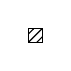
\begin{tikzpicture}[x=1.2ex,y=1.2ex]
        \filldraw[pattern=north east lines](0,0)rectangle(1,1);
      \end{tikzpicture} = Logistic,
      \begin{tikzpicture}[x=1.2ex,y=1.2ex]
        \filldraw[pattern=dots](0,0)rectangle(1,1);
    \end{tikzpicture} = MLP) \\
    \midrule
    & \multicolumn{4}{l}{Majority class (Inflection)} & \otherchart{0.57}                  \\
    \hdashline
    & \chgform & –       & –        & –               & \chart{0.58}{0.01}{0.58}{0.01}     \\
    & –        & \chgemb & –        & –               & \chart{0.66}{0.01}{0.66}{0.01}     \\
    & –        & –       & \varform & –               & \chart{0.68}{0.01}{0.68}{0.02}     \\
    & –        & –       & –        & \varemb         & \chart{0.73}{0.01}{0.74}{0.01}     \\
    \rowcolor[gray]{0.9}[4pt]
    (A) & –        & –       & \varform & \varemb         & \chart{0.83}{0.01}{0.83}{0.01}     \\
    \arrayrulecolor{white}\hline\hline
    \rowcolor[gray]{0.9}[4pt]
    (B) & \chgform & \chgemb & –        & –               & \chart{0.67}{0.01}{0.67}{0.01}     \\
    \hline\hline
    \rowcolor[gray]{0.9}[4pt]
    (C) & \chgform & –       & \varform & –               & \chart{0.69}{0.01}{0.73}{0.01}     \\
    \hline\hline
    \rowcolor[gray]{0.9}[4pt]
    (D) & –        & \chgemb & –        & \varemb         & \chart{0.75}{0.01}{0.78}{0.01}     \\
    & \chgform & –       & –        & \varemb         & \chart{0.73}{0.01}{0.75}{0.01}     \\
    & –        & \chgemb & \varform & –               & \chart{0.73}{0.01}{0.73}{0.01}     \\
    & \chgform & \chgemb & \varform & –               & \chart{0.73}{0.01}{0.77}{0.01}     \\
    & \chgform & \chgemb & –        & \varemb         & \chart{0.76}{0.01}{0.81}{0.01}     \\
    & \chgform & –       & \varform & \varemb         & \chart{0.83}{0.01}{0.84}{0.01}     \\
    & –        & \chgemb & \varform & \varemb         & \chart{0.83}{0.01}{0.85}{0.01}     \\
    \rowcolor[gray]{0.9}[4pt]
    (E) & \chgform & \chgemb & \varform & \varemb         & \boldchart{0.83}{0.01}{0.89}{0.01} \\
    \arrayrulecolor{black}\bottomrule
  \end{tabularx}
  \caption{\added[id=r2]{Cross-validation accuracy and standard error} in reconstructing UniMorph's inflection–derivation distinction by various supervised classifiers. \added[id=r2]{Linguistically-motivated hypotheses referred to in the text are denoted with letters}}
  \label{tab:featresults}
\end{figure}

While our best logistic classification model can capture 26 points of variation more than predicting the majority class, it may be missing non-linear interactions between independent variables, or between an individual independent variable and the dependent variable.
To account for such non-linear relationships, we fit a multi-layer perceptron (MLP) with a hidden layer size of 100, using the Adam optimizer \citep{kingma-et-al-2015-adam} and training for 3000 steps. The number of layers and layer size was selected using validation set performance, while the number of steps was chosen based on loss convergence on the training set. We find similar patterns of performance for most combinations of predictors. However, we see substantial improvements in performance for combinations of features which include \added[id=r2]{both magnitude and variability features}; for example, $\big(\chgform,\varform\big)$ improving from $69 \pm 1\%$ to $73 \pm 1\%$. Perhaps as a result of this, we achieve a test-set accuracy of $89\pm 1\%$, when using all four predictors---representing a 6-point improvement over the best linear model, as well as a 4-point improvement over the best combination of three measures using the MLP $\big(\chgemb,\varemb,\varform\big)$. This therefore suggests that while the variability features are the most descriptive of UniMorph's categorization of inflection/derivation, all four features contain unique information relevant to recreating this distinction (Hypothesis E).

\section{Classification of Linguistic Types of Inflection}
\label{sec:canon}
Given the controversy over what should be considered inflection and derivation, a model that largely aligns with a typical operationalization of the distinction (UniMorph 4.0) may also be of interest in the ways in which it {\em differs} from that operationalization. Accordingly, in this section, we look at the trends in how our model classifies constructions which are labelled as inflection in UniMorph.
\added{We consider several distinctions which we believe to be of linguistic interest, specifically: what kind of meaning is expressed by an inflection; whether it is {\em transpositional} (changes the part of speech); and whether it is {\em contextual} or {\em inherent} (as described by \citealt{booij-1996-inherent}). We ask whether these distinctions affect how likely an inflectional construction is to be classified correctly under our best model (the MLP with all four measures). We focus only on inflectional constructions because UniMorph has cross-linguistically consistent featural annotations on inflections that we can use for the analysis; no such cross-linguistically consistent annotation exists for derivation.
}

\subsection{Categories of inflectional meaning}
We first consider several categories of inflectional meanings: features for mood (e.g. indicative, subjunctive); tense (present, past...); number (singular, dual, plural...); voice (active, passive); comparison (comparative, absolute/relative superlative, equative); gender, and case. These categories of meaning are often used to structure accounts of inflection, such as UniMorph's description of its feature set \citep{sylak-glassman-2016-composition} as well as theoretical accounts like
\citet{anderson-1985-inflectional} and even \citeauthor{haspelmath-2024-inflection}'s (\citeyear{haspelmath-2024-inflection}) retro-definition of inflection. \added{It is, however, worth noting that} not all sources agree on all of these categories \added{as being inflectional. For example,} Haspelmath rejects voice as inflectional, and comparison is \added{often omitted from discussions of} major cross-linguistic inflectional categories (as is the case in both \citealp{anderson-1985-inflectional} and even \citealp{haspelmath-2024-inflection}), and is considered {\em inherent inflection} (which is less canonical) by \citet{booij-1996-inherent}. One might reasonably expect constructions which \added{are semantically marked for} these controversial categories to be {\em more likely to be classified as derivation} by our model.

\added{Note that linguists generally agree on which categories of meaning are semantically marked across languages \citep{greenberg-1966-universals,silverstein-1986-hierarchy,croft-2002-typology,ackema-et-al-2019-default},
and semantic markedness often corresponds to morphological marking. For example, past tense is generally considered more semantically marked than present, and in many languages the past tense requires an affix while the present tense does not. However, the UniMorph annotations include both the semantically marked and unmarked inflections (e.g. V;PAST;PL and V;PST;PL for Ukrainian verbs).}
Therefore,
for the purposes of this analysis, we consider active voice, singular number, nominative case,\footnote{While some languages have been argued to mark for nominative case with accusative being unmarked \citep{konig-2006-marked} no such language is present in our study.} and present tense unmarked values, even when present in the featural description of a construction.
\added{For example, in Ukrainian verb annotations, V;PAST;PL would be considered marked for tense and number, while V;PST;SG would be considered unmarked for both; both verbs would be unmarked for voice and mood since these are not in the featural descriptions.}
For the category of gender, we simply consider nouns \added{not to be marked, as their gender is typically not a morphological process but a lexical property}.

\begin{figure}
  \centering
  \includegraphics[width=\textwidth]
  {figures/infder/odds.pdf}
  \caption
  {Probability and Odds ratio with 95\% confidence intervals of being classified as derivation  for various kinds of inflectional meaning. Inflections to the right of the dotted line were disproportionately likely to be classified as derivation by our model}
  \label{fig:odds_meaning}
\end{figure}

Figure~\ref{fig:odds_meaning} displays the probability that a construction marking for one of these inflection types will be classified as derivation by our best-performing model. As can be seen in the figure, our model does not classify any of these major kinds of inflection as {\em more derivational than inflectional}; each is substantially more likely to be classified as inflection than derivation. This finding is perhaps unsurprising given our model's cross-linguistic \added[id=r2]{test set} classification accuracy of 90\%---it classifies 92\% of inflections correctly in general. Accordingly, classifying just 15-20\% of constructions belonging to a particular inflectional category as derivations has the potential to be significant.

In order to answer the question ``Are constructions which mark for this inflection type significantly more  likely to be classified as derivational than others?'', we compute the odds ratio.
We focus on the best performing MLP model (using all 4 features) in these results, which are presented in Figure~\ref{fig:odds_meaning} with 95\% confidence intervals. Constructions with an odds ratio significantly greater than 1, while not more likely to be classified as derivation than inflection, can nevertheless be thought of as particularly {\em non-canonical} types of inflection under our model, while those with odds ratios significantly below 1 are {\em canonical} with respect to our model.

We apply the Boschloo exact test \citep{boschloo-1970-raised} to the results and correct for multiple comparisons with the Bonferroni correction, which yields a significance level of $0.05/7=0.007$.
We find the odds ratios for gender $(p=1\times10^{-7})$, tense $(p=3\times10^{-7})$, and mood $(p=1\times10^{-7})$
significant. This identifies gender, mood, and tense as particularly canonical inflectional distinctions under our model---all of which are well in line with the claims of Haspelmath and others.

While we do not identify any inflectional meaning categories which are significantly more likely to be classified as derivations than the average inflections, the categories of passive voice $(p=0.03)$ and comparatives $(p=0.08)$ each have 95\% confidence intervals which are almost exclusively larger than 1. Each of these categories has been discussed as less canonical kinds of inflection, with comparatives even occasionally being listed as derivations within UniMorph.\footnote{For example, they are listed as derivations in English, but as inflections in German.} As these are the two least common categories in our sample (consisting of just 57 comparative constructions and 41 passives), it may be that these effects would be significant with a larger sample; alternatively, their relatively high likelihood of being classified as derivation could be an artefact of their rarity in our sample.
\subsection{Inherent vs. contextual inflection and transpositions}
While we do not find any categories of inflectional {\em meaning} as non-canonical under our model, we also consider two other major categories of inflection that have been discussed in the linguistic literature as potentially non-canonical: inherent inflection and transpositions, for which results are displayed in Figure~\ref{fig:odds_other}.

\begin{figure}
  \centering
  \includegraphics[width=\textwidth]
  {figures/infder/odds_other.pdf}
  \caption
  {Probability and Odds ratio with 95\% confidence intervals of being classified as derivation  for inherent inflections and transpositions}
  \label{fig:odds_other}
\end{figure}

First, we consider \citeauthor{booij-1996-inherent}'s (\citeyear{booij-1996-inherent}) notion of inherent and contextual inflection.
\added{Booij describes contextual inflection as canonical: it is determined by the syntactic context in which a word appears and indicates agreement (e.g. plural marking on a verb, which is controlled by its subject). In contrast, inherent inflection is non-canonical: it contributes to the meaning of the word itself (e.g.\ the plural noun).}
To operationalize this in a simple, cross-linguistically consistent way, we associate number, gender, and case\footnote{\citet{booij-1996-inherent} makes the distinction between structural and semantic case, with the former being contextual inflection and the latter inherent. However, due to the complexity in drawing a line between these categories, we treat all case marking on nouns as inherent.} with nouns---meaning that when those features appear on other parts of speech, we consider them contextual inflections. Analogously, we associate mood, tense, and voice with verbs. We then may consider whether an inflection is {\em inherent} or not, where we define inherency as not marking {\em any} contextual features. As shown in Figure~\ref{fig:odds_other}, we find that inherent inflectional constructions are not more likely to be classified as derivation than inflection; however, they {\em are} significantly more likely to be classified as derivation compared to other types of inflections, as quantified by the odds ratio $(p=6\times10^{-9})$. Interestingly, though, we find this to be almost entirely due to nominal inherent inflection $(p=2\times10^{-8})$, rather than verbal inherent inflection $(p=0.7)$. We see this exemplified in Figure~\ref{fig:odds_inher}, which shows that inherent case is significantly associated with being classified as derivation $(p=1\times10^{-5})$, while contextual case $(p=0.003)$ and contextual number $(p=0.0008)$ are significantly associated with being classified as inflection.

\begin{figure}
  \centering
  \includegraphics[width=\textwidth]
  {figures/infder/odds_inher.pdf}
  \caption
  {Probability and Odds ratio with 95\% confidence intervals of being classified as derivation  for inherent vs. contextual noun inflections}
  \label{fig:odds_inher}
\end{figure}

Finally, we consider inflectional transpositions, denoted in UniMorph as participles (deverbal adjectives), converbs (deverbal adverbs), and masdars (deverbal nouns), shown in Figure~\ref{fig:odds_other}. Transpositions have often been argued to be non-canonical inflection or even derivation because transpositions change the part of speech \citep{spencer-2013-lexical, plank-1994-inflection, haspelmath-2024-inflection}. We here find under our model that transpositions appear neither significantly more or less likely to be classified as derivations than inflections by our model---neither particularly canonical nor non-canonical. This may be due to the non-contextual nature of our embedding model: many inflectional transpositions are syncretic with a non-transpositional form, and our model must assign these the same location in embedding space. Thus, our null result here should not be taken as strong evidence against considering transpositions as non-canonical.

\subsection{Summary}

\added{In this section, we have investigated different kinds of inflectional constructions discussed in the linguistics literature to see whether any of these are particularly {\em canonical} or {\em non-canonical} under our model. That is, we looked at whether our model is more (or less) likely to correctly classify these constructions as inflectional, relative to the average inflectional construction.}

We identify mood, tense, and gender as {\em canonical inflections} under our model, but we do not find any categories of inflectional meaning which are significantly {\em non-canonical} in our sample. We find that inherent inflections are significantly more likely to be classified as derivations, in line with \citeauthor{booij-1996-inherent}'s (\citeyear{booij-1996-inherent}) view of them as non-canonical inflection.  Interestingly, we find this is driven by inherent nominal inflections rather than inherent verbal inflections. Finally, we investigate transpositions (typically thought of as non-canonical inflection), finding no evidence that they are either canonical or non-canonical under our model.

\section{Discussion}

\subsection{The role of our individual measures}\label{sec:featureimp}
As shown in Section~\ref{sec:classify}, all four of our measures can be used to achieve better discrimination between traditional concepts of inflection and derivation; however, not every feature plays an equally large  role. In this section, we discuss the roles played by each of our features and their connection to linguistic theory.

Among our four measures, our results point to variability of the change in distributional embedding \varemb being the most relevant to traditional categorizations of inflection and derivation. This is in line with the findings of \citet{bonami-et-al-2018-inflection} and \citet{copot-et-al-2022-idiosyncratic} in French, who focus on similar measures as a proxy for semantic drift, as part of a theory where traditional concepts of inflection and derivation reflect higher or lower {\em paradigmatic predictability}. Indeed, it is possible that this measure could be (roughly) equivalent to \citeauthor{copot-et-al-2022-idiosyncratic}'s (\citeyear{copot-et-al-2022-idiosyncratic}) predictability of frequency, as it is motivated from a similar theoretical basis. On the other hand, our measure is much simpler to define and compute: attempting to produce a measure of {\em predictability} immediately raises complex issues around on {\em what basis} such predictions should be made, complicating the interpretation of results.

In addition, we find a clear and complementary influence of the variability of the change in form, \varform: adding this feature to our model produces a large increase in performance, even when \varemb is already included. This measure \added[id=r2]{(described in Section~\ref{sec:ortho})} can be thought of as \replaced[id=r2]{a weighted measure of allomorphy, capturing not just the number of distinct patterns, but also their similarity}{describing the complexity of the structural relationship between base forms and constructed forms}. Our results point to \replaced[id=r2]{a much higher degree of formal variability/allomorphy for inflections than derivations}{this relationship being much more complex for inflections than derivations} across a wide range of languages, contrary to the predictions of \citet{plank-1994-inflection} and \citet{dressler-1989-prototypical}, but in line with the argument in~\cref{sec:formal-dim}. Although work on French has suggested little difference in the {\em predictability} of form for derivational and inflectional constructions \citep{bonami-et-al-2019-paradigm}, we clearly find within our sample of languages evidence that the {\em actual degree of variation} is very different.

Superficially, this finding could appear to be caused by the fact that derivational allomorphs are sometimes not collapsed in UniMorph data (e.g. \textit{–heit} and \textit{–keit} being listed as different morphemes in German). However, when we looked into this issue, we found that most derivations had 0–1 such uncollapsed allomorphs. Combining two allomorphs in this way would add at most half the edit distance between the morphs to our measure. In most cases, the edit distance between these allomorphs is 1–2, adding just $0.5$–$1.0$ to the value of \varform. This is much less than the difference between the means of the two categories in this feature, suggesting that failure to collapse allomorphs is not the primary source of this finding. Returning to the example of {\em –heit} and {\em –keit} within German, we find {\em –heit} has \varform of 1.53 and {\em –keit} has \varform of 1.25. The two morphemes occur 27\% and 73\% of the time respectively. When combined, they have a \varform of 2.43–--still well within the derivational range.

\added{Similarly, one might object that not only such straightforwardly-conditioned allomorphs must be accounted for, but also more idiosyncratic variants that express the same meanings. For example, in French, such formally distinct forms as {\em -age}, {\em -ance}, and {\em -ure} could be argued to be allomorphs of a single action-noun forming morpheme. \citet{copot-et-al-2022-idiosyncratic} handle this by grouping morphemes with similar semantics, by computing average difference vectors in embedding space between base and constructed form for each morpheme, and agglomeratively clustering morphemes with difference vectors with cosine similarity over 0.7. We find such clustering of our data \deleted[id=r2]{is} does not sufficiently align with semantic categories of morphemes across our full range of languages to reformat our analysis around it. However, even when clustering derivations with  this threshold of similarity, we still find a much lower degree of formal variability  for derivations than inflections. On average across languages, 38\% of derivational constructions cluster with nothing else at all, without increasing variability. The average cluster contains just 1.8 morphemes, with  inflectional morphemes, which are not clustered in this way, exhibiting still 208\% more allomorphs on average than derivational clusters.}

Future studies should explore the relevance of the variability of form further, to see if it is robust to different languages, and focus directly on the validity of this measure. However, we note that our best performing model without this feature, the MLP with the features $\big(\chgform, \chgemb, \varemb \big)$ achieves a classification accuracy of $81\pm 1\%$, which is still 23 points above predicting the majority class.

Finally, our results show smaller influence of the magnitude measures \chgform and \chgemb. This finding seems to contrast with Spencer's general claim that derivations are associated with larger changes to the properties of a lexeme, but it is not entirely contradictory. In particular, \chgemb still displays a fairly strong correlation with inflection and derivation on its own, and likely does not contribute as much to our models due to its substantial correlation (Pearson's $r$: 0.86) with the more strongly predictive \varemb. In the case of \chgform, we find little evidence here that derivations have a tendency to produce larger changes to the form; however, this may be in part related to our need to remove constructions which are orthographically syncretic between the base form and constructed form (which are dominantly considered inflectional in our sample of languages). The length of the change in form does seem to play a small role as a part of a composite set of factors based on its use in our best-performing MLP model.

\added{As noted in Section~\ref{sec:embedding}, our use of FastText somewhat complicates the interpretation of the role of the distributional measures, in the sense that embeddings based on sub-words may capture some formal similarity between words as well as semantic and syntactic similarity. However, we note that if the embeddings do capture formal similarity, at least some of this information must be complementary to that captured by our form-based measures, since including both types of features yields a better classifier than either alone. We also performed some supplementary experiments with Word2Vec embeddings to check that distributional features without sub-word information are also useful.}\footnote{For more details about these experiments, see Appendix~\ref{app:word2vec}.} \added{While overall performance of the classifier was lower (likely due to overall worse quality of the embeddings, for the reasons described in Section \ref{sec:embedding}), we still found a non-trivial contribution from the distributional features.
So, while we can say that both formal and distributional properties are associated with the inflection-derivation distinction, further work is needed to clearly distinguish semantic, syntactic, and formal properties.}

\subsection{Language generality}\label{sec:langgen}
An important aspect of our model is its lan\-guage-ge\-ne\-ra\-li\-ty. A major limitation of existing computational studies of the in\-flec\-tion–derivation distinction \citep{copot-et-al-2022-idiosyncratic,rosa-et-al-2019-attempting,bonami-et-al-2018-inflection} is their focus on single European languages. In particular, \citet{haspelmath-2024-inflection} argues that many properties of inflection and derivation are not proven to apply in a consistent way across languages (especially non-European and non-Indo-European languages). Our model achieves high accuracy across languages, while using no language-specific features. As such, it suggests that across the languages in our sample, inflection and derivation show cross-linguistically similar distributional properties.

Given the large number of European languages in our sample, this result clearly suggests that, at least in the Indo-European family, inflection and derivation are associated with distinct signatures in terms of both their distribution and their form (at least, as expressed in orthography). While evidence for such claims has been provided in specific languages by \citet{copot-et-al-2022-idiosyncratic}, \citet{bonami-et-al-2018-inflection}, and \citet{rosa-et-al-2019-attempting}, many large subfamilies within the Indo-European language family had previously been untouched by this literature. Our study includes several Germanic languages with distinctive morphological traits, as well as
Armenian, Latvian, Irish, and Greek, covering many smaller European branches of the Indo-European family.
We also expand the evidence for consistency in the application of the terms ``inflection'' and ``derivation'' within the Romance and Slavic language families. This broad coverage overall provides quantitative evidence for the cross-linguistically consistent application of the inflection–derivation distinction within the languages of Europe---not only in terms of the morphosyntactic traits of these constructions, as framed by \citet{haspelmath-2024-inflection}, but also in terms of corpus-based measures which are a proxy for the linguistic intuitions and subjective tests Haspelmath argues should be abandoned.

In addition to this robust evidence that these properties can discriminate inflection and derivation within Indo-European languages, we also show evidence of a degree of applicability to a wider range of languages.
On this subset of languages, our best MLP classifier averages 82\% accuracy on the test set, lower than for the Indo-European languages (average 91\% accuracy).
While this is still well above the majority class baseline (74\% accuracy on this subset), it suggests that the application of the inflection–derivation distinction to non-Indo-European languages may indeed be less consistent, as suggested by Haspelmath. Of particular note are the \deleted{low} results for Turkish. Turkish is a highly agglutinative language with, according to traditional descriptions, an exceptionally rich inflectional system---reflected by an extremely large number of inflectional constructions and relatively small number of derivations in our dataset. Our classifier over-uses the label derivation for this language---classifying all derivations correctly, but also classifying many inflections as derivations. This suggests a misalignment between the orthographic and distributional tendencies observed in European languages, and the way linguists typically operationalize inflection and derivation in this language. On a theoretical level, then, our results are therefore compatible with either a view where we should think of some of these so-called inflections in Turkish as more derivational, or a view where these corpus-based measures are less accurate indicators of what ``should'' be considered inflection for Turkish.

Due to the relatively small number of non-Indo-European languages and constructions from these languages we are able to consider in the present work, we are unable to draw definitive general conclusions about cross-linguistic consistency in our measures with languages outside Europe. Our results here seem to point to an intermediate view where these corpus-quantifiable correlates of inflection and derivation are {\em less reliable} descriptors of the way the distinction is made outside of Indo-European languages but still explain {\em substantial amounts} of the distinction.

\subsection{The classification approach}\label{sec:whyclass}

Another key differentiating aspect of our work from previous computational studies is our focus on classification of constructions. This method allows us to quantify {\em how much} of the inflection–derivation distinction, as operationalized across a wide range of languages, can be explained by our simple set of corpus-based correlates. Our focus on a wide range of languages necessitates the use of a quantitative method such as classification, and contrasts with the single-language studies of \citet{bonami-et-al-2018-inflection} or \citet{copot-et-al-2022-idiosyncratic}, who focus more on discussing individual constructions.

Further, our goal of looking at whether {\em multiple features} produces a more clear-cut and less gradient view of inflection compared to the single correlates examined by \citet{bonami-et-al-2018-inflection} or \citet{copot-et-al-2022-idiosyncratic} prevents us from simply doing a statistical test of correlation between a feature and inflection/derivation. While we avoid this by training a classification model, \citet{rosa-et-al-2019-attempting} solve this problem by using clustering. We believe doing so conflates two questions about the measures under consideration. First is the question of how {\em consistent} linguists' categorizations are in terms of the measures. Secondly, there is the question of how {\em natural} the traditional categories of inflection and derivation appear with respect to these measures. This first question is a lower bar than the latter: it may be possible to use these measures to determine inflectional or derivational status, regardless of whether they form natural clusters in the feature space.

Nevertheless, a finding of {\em consistency} without {\em naturalness} is still interesting, given that decisions about what to consider inflection and derivation were made without access to these measures. For example, consistency with respect to these measures could make them a successful ``retro-definition'' in the terms of \citet{haspelmath-2024-inflection}. The clustering approach may also fail to identify a distinction where inflection and derivation are predominately located in only slightly overlapping regions of the feature space but do not necessarily form natural clusters.\footnote{As described in Section~\ref{sec:grad} and shown in Figure~\ref{fig:gradient}, it is this situation in which we find ourselves.} It is this question of consistency which we primarily consider in this paper, leading us to eschew the unsupervised clustering approach for supervised classification.

Another advantage of our focus on classification is that it naturally lends itself to testing the {\em generalizability} of our claims: by holding out a random subset of our constructions for testing data and computing accuracy on that set, we confirm that our results do not over-fit to the constructions in the training set.

\subsection{Inflection and derivation: gradient or categorical?}\label{sec:grad}
Whether the inflection–derivation distinction is principally a gradient or categorical phenomenon is a long-standing debate within linguistic theory with potentially wide-ranging implications about the nature of linguistic representations. Many theories of morphological grammatical organization, production, and processing implicitly or explicitly employ the ``split morphology hypothesis,'' which holds that inflection and derivation are separated in the grammar \citep{perlmutter-1988-split,anderson-1982-wheres}. Those who propose such separate structures rely on both the distinction between inflection and derivation being discrete and the specifics of that distinction---i.e., what morphological constructions in what languages are considered either inflectional or derivational.

On the other hand, a growing body of linguistic theory rejects a hard distinction \citep[e.g.][]{bybee-1985-morphology,spencer-2013-lexical,dressler-1989-prototypical,stekauer-2015-delimitation,corbett-2010-canonical,bauer-2004-function}. In its place, they often treat inflection and derivation as a gradient, perhaps emergent out of deeper phenomena. This view has been borne out in the computational work of \citet{bonami-et-al-2018-inflection} and \citet{copot-et-al-2022-idiosyncratic} who find clear continuous gradience with respect to their metrics and the categories of inflection and derivation.

While, as discussed in \ref{sec:whyclass}, we focus primarily on the {\em consistency} of traditional categories of inflection and derivation, in this section we briefly investigate whether, under our measures, the distinction between inflection and derivation appears more {\em gradient} or more {\em categorical}. If the former is the case, we expect a relatively even distribution of constructions in feature space, which (perhaps gradually) transition from being traditionally classified as inflection to being traditionally classified as derivation. In the categorical case, however, we expect {\em clusters} within feature space with relatively few constructions lying in intermediate ambiguous regions.

We focus on four measures in this study, so we are unable to directly visualize in the feature space. While we applied principal component analysis to produce a two-dimensional representation of our full feature space, the principal components did not pattern into inflectional and derivational regions. This is certainly evidence against  {\em naturalness} of the traditional distinction with respect to our measures. However, we may also look at our two most strongly predictive measures, as shown in Figure~\ref{fig:gradient}. Recall that a logistic classifier using only these features was able to correctly classify \added[id=r2]{$83\pm 1\%$} of constructions. Our results with our measures are here consistent with the existing findings of a gradient, rather than categorical, distinction between inflection and derivation with respect to traditional linguistic tests/measures which operationalize them---we observe a spread of constructions in the two-dimensional feature space with a smooth transition between regions containing almost exclusively inflections and regions containing almost exclusively derivations.

\begin{figure}
  \centering
  \includegraphics[width=0.8\textwidth]{figures/infder/gradient.pdf}
  \caption
  {Our two most predictive measures for inflection and derivation. \added{Saturation represents overlapping constructions.} With respect to these two variables, the inflection–derivation distinction appears gradient rather than categorical}
  \label{fig:gradient}
\end{figure}

\subsection{Are inflection and derivation identifiable from the statistics of language?}
In this work, we have focused on identifying cross-linguistically applicable corpus-based measures, which have a consistent relationship with the traditional concepts of inflection and derivation. While we have primarily motivated the use of these corpus-based measures in terms of quantifying how consistently these categories are applied across languages or making concrete subjective linguistic tests, the fact that they are built purely from the statistics of natural language corpora allows us to consider another important question: is the inflection-derivation distinction something which is present in the statistics of language itself?

If the retro-definition given by \citet{haspelmath-2024-inflection} is the right one, for instance, the answer to this question would superficially appear to be {\em no}. Haspelmath casts the distinction in terms of morphosyntactic feature values, which themselves refer in many cases to the {\em meaning} expressed by a morphological exponent. If the specific meaning expressed by a morphological relation is necessary to distinguish which relations are inflectional in nature and which are derivational, then the typical inflection–derivation distinction requires {\em grounding} the meanings of sentences to solve---for example, no amount of raw \replaced{text}{language} input in a language can tell you whether the relationship between two words is ``agentive'' or ``plural.''

The answer to this question has implications within psycholinguistics as well as computational linguistics.  Psycholinguistics provides some empirical evidence that inflection and derivation are processed differently \citep{laudanna-et-al-1992-processing, kirkici-et-al-2013-inflection}, which seems to imply learners have some implicit ability to categorize constructions into inflection and derivation. How might a learner learn what processing to apply to a given morphological construction in this case?
A substantial body of literature indicates that humans can and do perform purely statistical learning within language acquisition \citep{swingley-2005-statistical, saffran-et-al-1996-statistical, thiessen-et-al-2013-extraction, thompson-et-al-2007-statistical, thiessen-et-al-2003-when}. Without using or even having access to the references of sentences in some cases, learners uncover important aspects of the structure of language. Our results therefore suggest the possibility that statistical learning may play a role in learning to process canonical inflection differently from canonical derivation.

This is also relevant for the validity of several constructs within natural language processing. For example, the paradigm clustering task from SIGMORPHON 2021 \citep{wiemerslage-etal-2021-findings}, which requires identifying inflectional paradigms from raw text, can only be solved if inflections and derivations can be distinguished from the \replaced{statistics of such a corpus}{linguistic signal itself}. Otherwise, derivational relations would be outputted by even the best possible system. Similarly, the task of unsupervised lemmatization \citep{kasthuri-et-al-2017-plis, rosa-et-al-2019-unsupervised} also relies on the distinction between inflection and derivation being evident \replaced{within a text corpus}{from the linguistic signal}. Our results point to these types of construct being largely valid for Indo-European languages given the high degree of discriminability between the categories, but our slightly lower results for non-Indo-European languages suggests the need for further investigation into the validity of such constructs for typologically-distant languages to those considered here.

\subsection{Classification and syntactic change}\label{sec:synoracle}
\textcolor{red}{To place an upper bound on how many of the model's errors can be explained by syntactic information, we consider how many errors can be explained by a syntactic change oracle variable. Using the annotations for part of speech in UniMorph, we produce a binary variable for whether a given construction changes the part of speech, using the start and end parts of speech for derivations. For inflections, we assume the part of speech does not change unless it is annotated by UniMorph as one of a participle, masdar, or converb. We add this oracle variable to the input to the classifier. We achieve a test-set accuracy of 84\% with the logistic classifier and 92\% with the MLP when combined with our four distributional measures. This represents a performance decrease of 2 points and increase of 2 points, respectively, suggesting little-to-no improvement to be found by a feature so closely aligned to linguistic notions of a change in part of speech.}

\textcolor{red}{However, this oracle measure captures only a very restricted notion of syntactic change: change in coarse-grained part of speech. For instance, while we treat inflectional transpositions, such as participles, as changing the part of speech in the creation of our oracle variable, this is a contentious point due to some syntactic similarities they share with verbs, which might be reflected in such a measure. On the other hand, some derivations which do not change part of speech may nevertheless change something about the syntactic context (e.g. verbal argument-structure alterations or passive constructions), and may thereby yield greater values in such a measure. A more fine-grained syntax measure which captures this might map more neatly onto the categories of inflection and derivation.
Finally, since UniMorph part-of-speech annotations are only at the construction-level, there is no variability in this syntactic information; a distributional account of syntactic information could represent individual pair variation within a construction (due to semantic drift, for example), which might be informative for reconstructing the distinction.}

\textcolor{red}{Despite these caveats, these results suggest that syntactic transposition has little added predictive power over and above our corpus-based measures. This is in line with a view of the inflection-derivation distinction where syntactic change is not definitionally related to the distinction, but epiphenomenally correlated with it.}

\subsection{Future work}
We believe our study presents a number of interesting avenues for expansion. One such possibility is the extension of the present work to a larger and more diverse sample of languages. In this work, we have taken advantage of the recently produced UniMorph 4.0 dataset to validate claims based on individual languages that corpus-based measures can capture traditional notions of inflection and derivation, and quantify how many intermediate constructions exist under such measures, but our results mostly bear on languages of Europe belonging to the Indo-European language family. While this still represents a substantial advancement in knowledge, and we do find some evidence that our results are applicable to non-Indo-European languages (as described in Section~\ref{sec:langgen}), the evidence presented here cannot yet fully refute \citeauthor{haspelmath-2024-inflection}'s (\citeyear{haspelmath-2024-inflection}) claim that inflection and derivation are much less applicable to languages outside Europe. Relatively few (590) of the constructions in our data belong to non-Indo-European languages, with even fewer (201) coming from languages spoken outside Europe, and no representation of languages from outside Eurasia. As argued by \citet{dryer-1989-large}, typological claims must be made not just with normalization with respect to language families or small geographical areas, but even large geographical areas---which is not possible with available data.  In order to properly understand to what degree the concepts of inflection and derivation map onto language generally, there is a critical need for the expansion of resources like UniMorph 4.0 and Universal Derivations \citep{kyjanek-et-al-2020-universal} to cover a larger and more representative set of languages. While UniMorph increasingly covers the inflectional morphology of a wide range of languages throughout the world, having added 65 languages from 9 non-European language families in the 4.0 release alone, no unified derivational resource covers a large number of non-European languages. The harmonization and integration of resources like derivational networks such as Hebrewnette \citep{laks-et-al-2022-hebrewnette} and finite-state morphological transducers which cover derivation such as \citet{arppe-et-al-2014-finitestate}, \citet{larasati-et-al-2011-indonesian}, \citet{strunk-2020-finitestate}, or \citet{calderonvilca-et-al-2012-analizador} into multilingual resources is essential to answering truly general typological questions with these resources in the future.

\added{Another limitation of this study that future work could address is indeed our use of the UniMorph 4.0 dataset. While UniMorph 4.0 provides the largest-scale multilingual dataset of inflection and derivation presently available, it is limited by factors related to its semi-automated construction, which may affect the way allomorphy is represented (as discussed in Section~\ref{sec:featureimp}), or other as-of-yet undiscovered systematic biases.}\footnote{\added[id=r2]{See \citet{malouf-et-al-2020-lexical} for a discussion of potential pitfalls of the UniMorph dataset for typological research.}
UniMorph represents not exactly a consensus of highly-trained linguists, but rather largely of the amateur lexicographers that make up the Wiktionary community. Accordingly, as more large-scale multilingual datasets are available, future work should investigate the degree to which these findings are robust to the method of data collection as well as the source of the data.}

Additionally, we have limited ourselves to a small set of measures here. Future work could seek to improve these measures, or look at other or additional measures. \replaced{Many previously suggested properties of these categories, such as affix ordering, have directly observable effects on the statistics of text.}{As shown in Table~2 we believe as many as 20 of Plank's subjective tests should have directly observable effects on the statistics of raw text.}
Future works could test corpus-based measures of distance from the stem or limitedness of applicability, for example. Particularly interesting, we believe, would be the investigation of a syntactic distance and variability component, drawing on works such as \citet{he-et-al-2018-unsupervised} and \citet{ravfogel-etal-2020-unsupervised}---though there are significant challenges to operationalizing these embeddings in a multilingual, low-resource domain.

There is also room for refinement of our measures \added{and classification techniques}. For example, extension to many other languages would likely require a re-assessment of our use of orthography as a proxy for linguistic form. The assumption that orthography is a reasonable proxy for form is not accurate in many languages---however, at present UniMorph does not include phonological transcriptions, and automated grapheme-to-phoneme conversion across a broad range of languages is the subject of very active research \citep{ashby-etal-2021-results}. These difficulties would need to be overcome in order to use phonological transcriptions. Future work should also investigate to what degree our variability of embedding measure is equivalent to or complementary to \citeauthor{copot-et-al-2022-idiosyncratic}'s (\citeyear{copot-et-al-2022-idiosyncratic}) predictability of frequency measure, as both are motivated from semantic drift due to a change in lexical index. Similarly, future work could \added{clarify the contribution of distributional semantics by using a model such as Word2Vec or GloVe}, or newer models of distributional semantics, such as XLM-R \citep{conneau-et-al-2020-unsupervised}---though in the latter case they would have to overcome the difficulties of multilingual decontextualization as described in Section~\ref{sec:embedding}. \added{Further, as we use only two simple classification techniques (logistic regression and an MLP), it is possible that further hyperparameter tuning or use of other techniques, such as random forests or gradient boosting, could improve on classification accuracy.}

\section{Conclusion}
In this work, we have presented the first multilingual computational study of the inflection–derivation distinction. In Section~\ref{sec:distributional} we define a small set of measures capturing the hypothesized tendency of derivation to produce bigger and more variable changes to the base form in terms of form, syntax, and semantics. We then systematically study the relationship between these measures and traditional categorizations of morphological constructions into inflection and derivation, which we derive from the UniMorph 4.0 dataset. In Section~\ref{sec:individual}, we show that these measures each correlate, in some cases strongly, with whether a construction is listed as inflectional or derivational in UniMorph 4.0. We show evidence that these correlations are not due to systematic differences in the frequency of inflectional and derivational constructions. In Section~\ref{sec:classify}, we show that both logistic regression and multi-layer perceptron classifiers which use these measures as inputs can be trained to reconstruct most of the UniMorph inflection–derivation distinction, with logistic classifier achieving a classification accuracy of $83\pm 1\%$ and the MLP achieving a classification accuracy of $89 \pm 1\%$, improving by 26 and 32 points over predicting the majority class, respectively. We identify the variability of the change in distributional embedding space \varemb and the variability of the change of form \varform as particularly strong correlates of the distinction, together able to classify $83\pm 1\%$ of constructions as they are classified in UniMorph.

Overall, these results show that much of the categories of inflection and derivation as used \replaced{in UniMorph}{by linguistic resources} can be accounted for by corpus-based measures which make concrete the subjective tests suggested by linguists. In so doing, we have also validated in a larger, multilingual context the core findings of \citet{bonami-et-al-2018-inflection} and \citet{rosa-et-al-2019-attempting}, finding that these properties hold across 26 languages (21 Indo-European and 5 others), with a model that uses no language-specific features. These well-defined, empirical measures avoid the often-discussed subjectivity and vagueness of existing criteria \citep{haspelmath-2024-inflection,plank-1994-inflection,bybee-1985-morphology}, and enable us to produce the first large-scale quantification of how consistently the categories of inflection and derivation are applied, and validate that these measures can {\em generalize} to unseen constructions.

With these measures, we are also able to identify in a quantitative way {\em how canonical} different categories of inflections are (Section~\ref{sec:canon}) in terms of properties of their form and distribution. We determine, that, as suggested by \citet{booij-1996-inherent}, inherent inflection is a {\em non-canonical inflectional category} under our model: inflectional constructions which are purely inherent are significantly more likely to be classified as derivations than other inflections under our model. We find in our sample this seems to be particularly due to {\em nominal} inherent inflections, like case and number. Furthermore, we find no traditional categories of inflectional meaning significantly non-canonical, providing some validation accounts of inflection which are structured around these categories like \citet{haspelmath-2024-inflection} or \citet{sylak-glassman-2016-composition}, though we find weak evidence that voice and comparatives could be such categories.

Finally, we note that while there is a high degree of consistency in the use of the terms inflection and derivation in terms of our measures and combining multiple measures reduces the amount of overlap between inflectional and derivational constructions, we still find many constructions near the model's decision boundary between the two categories, indicating a gradient, rather than categorical, distinction (Section~\ref{sec:grad}). This gradient region is relatively small, as suggested by our high accuracies, but does not suggest inflection and derivation as categories {\em naturally emerging} from our measures.

\subsection*{The view from lexicality}
\textcolor{red}{I now return to the broader questions and arguments in this thesis. The results in this study, finding a high degree of consistency in the application of the inflection--derivation distinction across a wide range of languages, suggest that the deployment of this distinction is perhaps somewhat less fraught than some have suggested \citep{haspelmath-2024-inflection, stekauer-2015-delimitation}, supporting cross-linguistic consistency in the application of this lexicality-related distinction. Further, the finding that a combination of corpus-based measures can reconstruct the inflection--derivation distinction with high accuracy, in addition to providing tools for analysing boundary cases, supports the argument in~\cref{ch:background} that defining a multidimensional empirical space for complex comparative concepts like inflection and derivation is a fruitful approach to understanding such concepts--similar to the development of empirical spaces for vowel typology or colour systems.}

\textcolor{red}{Do the results here support the view of inflection and derivation as a distinction of lexicality? The picture here remains somewhat mixed. We do see a moderate correlation of our measure of distributional change \chgemb with the inflection--derivation distinction, suggesting that derivations do tend to produce larger changes in distributional behaviour than inflections, as would be expected if derivations are more semantically contentful than inflections. However, this measure is highly correlated with and slightly less predictive than our measure of the variability of the change in distribution \varemb. This measure, inspired by ideas from the morphological literature about semantic drift and changes in lexical index, raises interesting questions about other levels on the lexicality continuum. If we think of inflectional and derivational constructions as two-item {\em compounds} between a lexical root and the morphological material, then the importance of \varemb could suggest that the lexicality of units at higher levels of formal structure (such as roots and words) could be reflected in the variability of distributional behaviour of these compounds. For example, the prediction is that meanings/distributions of noun--noun or adjective--noun compounds vary more than determiner--noun ``compounds''. (e.g. {\em red line} vs. {\em the line}). This would be an interesting avenue for future work.
}

\textcolor{red}{
  The contribution of the formal measures is also interesting from the perspective of lexicality. \chgform contributes very little to our best models, suggesting that the size of the change in form is not strongly related to the inflection--derivation distinction, and against the notion of lexicality as a correlation between formal size/length and semantic content. However, \varform is a useful predictor in our models, suggesting that inflections are more formally variable than derivations. Under the view I sketched in~\cref{sec:formal-dim}, this could be interpreted as inflections having less of a shared formal core than derivations, and being ``smaller'' in that sense. Overall, the results support a view of inflection and derivation as a complex combination of form and distribution, with some connections to semantic content.
}

% \section*{Acknowledgements}
% The authors would like to thank Paul J.W.\ Schauenburg, Albert Haley, Itamar Kastner, Kate McCurdy, and Francis Mollica for their comments on this work. This work was performed using resources provided by the Cambridge Service for Data Driven Discovery (CSD3) operated by the University of Cambridge Research Computing Service (\url{www.csd3.cam.ac.uk}), provided by Dell EMC and Intel using Tier-2 funding from the Engineering and Physical Sciences Research Council (capital grant EP/T022159/1), and DiRAC funding from the Science and Technology Facilities Council (\url{www.dirac.ac.uk}). This work was in part supported by the UKRI Centre for Doctoral Training in Natural Language Processing, funded by the UKRI (grant EP/S022481/1) and the University of Edinburgh, School of Informatics and School of Philosophy, Psychology \& Language Sciences.


\part{Word Classes}
% % Template for Edinburgh NLP
\chapter{Groundedness and the Lexical--Functional Distinction}\label{ch:grounded}
% \section{Introduction}
{
\color{red}


In the past century of linguistics, a key question has been whether language is characterized primarily as a formal system of signs abstracted from their signification, or as a functional system for communication. The former view has its roots in the \textsc{structuralist} tradition of Saussure \citep{desaussure-1916-cours}, and has been prominently represented in the \textsc{generative} tradition founded by Chomsky \citep{chomsky-1957-syntactic}. Beginning in the 1970s and 1980s, there was a reaction against this view, with the rise of \textsc{functional} and \textsc{cognitive} linguistics \citep[i.a.]{langacker-1987-foundations, givon-1979-understanding,haiman-1980-iconicity}, which emphasized the role of the communicative function of language, and the relationship between linguistic form and meaning. The latter view has gained substantial traction in recent years, with cross-linguistic work demonstrating the importance of functional pressures in shaping cross-linguistic patterns \citep{croft-2022-morphosyntax, givon-1979-understanding, stassen-1997-intransitive}, as well as language change and variation \citep{kirby-1999-function, croft-2000-explaining, zaslavsky-et-al-2018-efficient}.

Paralleling this, one of the most important mathematical advances in the twentieth century was the development of Shannon's \textsc{information theory} \citep{shannon-1948-mathematical}, which provided a framework for quantifying information. This framework has been widely applied to the study of language, especially by functionalists \citep{futrell-et-al-2022-information}. Yet Shannon's theory of information is fundamentally \textsc{structuralist} in nature; it is concerned with the statistical properties of symbols in a communications system, ignoring the signified. The Shannon's Information of a linguistic unit combines uncertainty due to both {\em what} is being expressed (function) and {\em how} it is being expressed (form). This entanglement is particularly problematic for cross-linguistic comparison, since form is language-specific.

Can we disentangle semantic contentfulness from linguistic form? This is made challenging by the empirical success of both information theory and the \textsc{distributional hypothesis} \citep{harris-1954-distributional}, which together suggest that meaning is inextricably linked to form. In Part I of this thesis, we explored the inflection--derivation distinction through the lens of distributional semantics. Because inflection and derivation are morphological processes which modify word form, using distributional representations from FastText allowed us to study this distinction through the geometry of word vectors. However, this approach entangles form and function; as shown in \cref{ch:corpus}, word vector similarities also include substantial syntactic information.

In this chapter, we propose a simple mathematical framework for separating form and function in the information-theoretic study of language. By introducing a language-neutral representation of meaning, we can quantify the information due to function alone, which we term \textsc{groundedness}. In this chapter, we specifically focus on \textsc{visual groundedness}: by looking at sentences produced as captions of the same image across languages, we can use the image as an evidence-based, language-agnostic representation of the shared semantics underlying these utterances.
}

Visual groundedness measures how much less surprising a word is when we know the perceptual stimuli (i.e., the image) it describes. This \textit{surprisal difference} between the surprisal of the word token in an image captioning model versus its surprisal in a language model is an estimate of the pointwise mutual information: the greater this difference (LM > captioning), the more \textit{grounded} the word is in that context.

%However, language is not just a formal system, but also a functional one.

% In recent years, text-based language models have exploded in popularity and performance, demonstrating not only a strong mastery of linguistic form, but also impressive abilities in terms of content, demonstrating a capability to answer questions which require world knowledge, apparent abilities to reason, and the ability to perform tasks not present in training data from examples shown at inference time (often called in-context learning). Yet these models also have a number of weaknesses which remain difficult to address. They are both incredibly parameter-heavy and data-hungry, and their apparent knowledge and reasoning abilities are highly variable across contexts. On the path to creating neural models with properties ever-closer to humans, one major direction which has emerged is the notion of {\em grounding} language models, by providing them not just with textual training data, but also some kind of world model with reference to which that textual data was produced. This has an intuitive appeal in several respects; the human learner of course receives not just language data, but simultaneous rich multimodal input in an environment with which they can interact; information which is often of use for learning language quickly, and information with which produced language is typically consistent. As such, it is natural to hope that models grounded in this way would improve in both language sample-efficiency and internal consistency.

% Nevertheless, achieving grounding is not straightforward; for example, the vast corpora used for training current state-of-the-art LLMs typically contain little-to-no relevant grounding information for their text. Further, ideas such as video-based grounding, while promising, are at present difficult to scale due to the incredibly high dimensionality of the data. As such, one simple multimodal grounding technique which is presently common is using a simple {\em image} as a proxy for the world model. Such an approach is promising in both in terms of computational efficiency and of ease of obtaining training data, as captioned images are relatively common e.g. on the web and in books. However, it represents a substantial simplification from human-like grounding. The question naturally arises: what does this grounding ground, and to what extent does it capture human grounding behaviors?

% \Edo{I wonder if it makes sense to start a step earlier and introduce the concept of grounded typology more broadly (as a way to `automate' the typological comparison based on function/semantics), and how it facilitates the study of word classes, then say we focus specifically on parts of speech.}

% Within linguistics, {\em typology} is the subfield focused on the study of patterns and variation across the world's languages \citep[pp. 1--2]{croft-2002-typology}. To identify such patterns, linguists must carefully identify phenomena of interest within languages, and then align them with one another.
% % \edo{Vowel typology is not a good example here, as phonetics can be compared based on form alone! We need an area where linguists posit functional constructions (e.g., possession, front information, etc) and then compare strategies that different languages use to express them. Better yet, let's use word classes as an example: we can refer to Talmy Givon's semantic categorisation based on time stability, etc}
%  For example, vowels exist in a continuous acoustic and perceptual space, without clear boundaries between them. To define vowel categories and align systems across languages, linguists rely largely on acoustic properties of the speech signal---reducing the problem to a physically grounded, empirical one \citep{liljencrants-et-al-1972-numerical, cotterell-eisner-2017-probabilistic}.

% While empirically grounding language form (surface structure like vowels) is typically straightforward, language is not just a formal system, but also a functional one. Many questions within typology relate to the relationship between form and {\em meaning}, especially in domains like morphology and syntax. Typically, typologists manually identify semantic/functional roles such as ``subject'', and ``causative'' and study their expression across languages \citep{haspelmath-2010-comparative, greenberg-1966-universals}. Unlike with many definitions based on form, definitions based on meaning are left up to subjective discretion, leading to debates which reduce to the definition of particular terms cross-linguistically \citep{haspelmath-2007-preestablished, haspelmath-2012-how, plank-1994-inflection}. %Further, this approach is not suitable for the {\em discovery} of functional roles, as it requires strict prior definition by a linguist.



% Instead, we propose a ``grounded'' approach to typology, which (under certain assumptions), allows the quantification and cross-linguistic comparison of language function and semantics across languages. s.

% In this work, we specifically focus on semantic contentfulness---how semantically informative a given word token is. We introduce a way to empirically quantify contentfulness, {\em groundedness}, which relies on vision-and-language models.

% The contemporary study of linguistic typology centers around defining precise, cross-linguistically applicable terms, and operationalising them across languages. This approach has yielded many successes in the domains of phonology, morphology, and syntax, but--similar to issues in formal linguistics more generally--can be challenging to apply to issues relating to (esp. lexical) semantics, which are resistant to formalisation. Finding utterances with cross-linguistically comparable meanings, and comparing them in a systematic way, remains an open problem. Traditionally, this has been achieved by the positing by linguists of abstract functions which often serve the role of systematising meaning.\edo{From a message I wrote in our chat:

% Traditionally, linguists have to posit abstract "functions/meaning" and then compare how languages vary in expressing them by inspecting utterances (speech or text). With grounded typology we can (albeit imperfectly) leverage measurable, quantifiable representations of meaning. So in a sense it 1) "automatises" to some extent the manual process of typological comparison. 2) enables us to study how forms vary in context. This also has important implications for the study or variation within languages.

% }

% In this work, we propose a ``grounded'' approach to typology, which (under certain assumptions) can allow the quantification and cross-linguistic comparison of semantic content across languages. By looking cross-linguistically at sentences produced as captions of the same image, we can use the image as a representation of the shared semantics underlying these utterances.

As a case study, we apply this measure to the study of the \textsc{lexical--functional distinction}. Literature from cognitive, pyscho- and neurolinguistics all point to contentfulness being an organizing factor in word class processing and even formation and structure: low-content (functional) word classes have many different properties from high-content (lexical) classes \citep{dube-et-al-2014-independent, bird-et-al-2003-verbs, chiarello-et-al-1999-imageability}. Yet, there has been no cross-linguistic study of the relationship between contentfulness and word class.

% Generally, a distinction is drawn in linguistics between closed-class and open-class parts of speech. Closed-class parts of speech do not admit new members and typically do not exhibit rich productive morphology; they tend to express highly grammaticalised and abstract meanings (think of determiners in English). Open-class parts of speech (like English nouns), can productively admit new members, and new members can often be formed by morphological means; and their meanings tend to be more concrete and contentful. Literature in psycho- and neurolinguistics points to factors like concreteness and imageability being highly relevant to word processing generally, and to assymmetries observed across and properties ascribed to word classes, such as assymetries in the processing of nouns and verbs in certain aphasias \citep{bird-et-al-2003-verbs, dube-et-al-2014-independent}.

%Imageability and concreteness ratings are typically produced through subjective human ratings, showing moderate correlations across languages \citep{rofes-imageability-2018}, and being limited in language and word availability---particularly limiting for typological studies, which require a diversity of languages. Additionally, some work in psycholinguistics has suggested that imageability and concreteness, though widely applied to the study of language processing, may actually be proxies for more fundamental, perceptually oriented variables that modulate lexical processing and the structure of word class \citep{connell-strength-2012}. While word classes are an area of substantial theoretical debate within typology \citep{bisang-word-2010, haspelmath-how-2012}, such properties have not been explored in a cross-linguistic manner due to these challenges.

Using our groundedness measure to quantify semantic contentfulness, we can estimate the mutual information of a word class with a caption's meaning (image). We find our measure largely rediscovers the distinction between lexical and functional word classes across 30 languages. Further, though it correlates only weakly with psycholinguistic norms for imageability and concreteness in English, it provides an intuitive ranking (noun > adjectives > verbs) across languages. On the other hand, it contradicts the view of adpositions as a ``semi-lexical'' class \citep{corver-et-al-2001-semilexical} and suggests grammatical word classes do carry some semantic content. These results thus partly validate and partly falsify received wisdom about word class contentfulness. They suggest the utility of this measure as a general tool for studying contentfulness in linguistics, and of taking a grounded approach to typological problems. We release the model used to estimate our measure and a dataset of groundedness values in 30 languages.\footnote{\url{https://osf.io/bdhna/}}

% In this study, we propose a grounded approach to typology, using images as a proxy for sentence meaning. Using information theory and neural models, we define a groundedness measure of a token's association with its meaning. Together, our results demonstrate that parts of speech vary systematically in terms of their groundedness across a typologically-diverse sample of languages. We find this variation can be described as a continuous cline generalizing the traditional distinction between lexical and functional word classes. However, our results suggest results suggest grammatical word classes still carry semantic content. We find that nouns > adjectives > verbs, in line with a continuum view of these classes, but our results contradict claims that adpositions are more lexical than other functional classes. Our measure is related to surprisal, but diverges from it, particularly for concrete words.
%A preliminary analysis suggests that the ways in which it deviates from existing measures make it interesting in its own right, prioritizing highly visually distinct concepts (like ``surfer'').
% This suggests the potential for this measure to provide a convergent type of evidence about the contentfulness of words, without requiring speaker involvement (shifting the requirement to organic text in a language and captions of images), and removing rater biases---all emergent from an image captioning/language modelling training objective.

%While classes like ``noun,'' ``verb,'' and ``adjective'' seem intuitive to speakers of Indo-European languages, they entangle a notion of syntax and semantics---an idea that words with a particular type of semantics should have a distinct, shared syntactic distribution. Within many of the world's languages, these categories are organized differently---with some languages (like Korean) not distinguishing between verbs and adjectives, some (like Japanese) having multiple parts of speech expressing adjectival meanings, and some (like Tagalog) argued not to distinguish noun and verb at all \citep{kaufman-2009-austronesian}.

% Motivated by this rich literature, we seek to develop an empirical {\em typology} of the relationship between word class and ``contentfulness''.

\section{Background}%\edo{Move part of intro here}
% \subsection{Typology}
% Within linguistics, {\em typology} is the subfield focused on the study of patterns which occur across the world's languages--that is, the facts examined within typology are cross-linguistic patterns \citep[pp. 1--2]{croft-2002-typology}. So while, for example, phonology may study the patterns of sounds within a language, phonological typology is concerned with cross-linguistic trends, generalizations, universals, and restrictions on sound patterns across languages. In order to identify such patterns, linguists must carefully specify systems of interest within languages, and then align them with one another.

% Take, for example, the typology of vowel systems. While dozens of acoustically distinct vowels exist, languages vary dramatically in both how many and which vowels they use, with some languages distinguishing as few as two vowels \citep{colarusso-northwest-1988} and others distinguishing as many as 46 vowels. Yet across the world's languages, vowel systems are not at all uniformly distributed. Most languages have systems with 5-7 vowels, and only an extremely small subset of possible 2, 3, and 4 vowel systems is attested \citep[p. 44]{gordon-phonological-2016}. Attested systems strongly tend e.g. to maximally separate the acoustic properties of their constituent vowels \citep{liljencrants-et-al-1972-numerical, schwartz-dispersionfocalization-1997}.
% % \edo{Vowel typology is not a good example here, as phonetics can be compared based on form alone! We need an area where linguists posit functional constructions (e.g., possession, front information, etc) and then compare strategies that different languages use to express them. Better yet, let's use word classes as an example: we can refer to Talmy Givon's semantic categorisation based on time stability, etc}

% Such generalisations about what sorts of vowel systems are attested across the languages of the world require defining cross-linguistically consistent categories. Vowels exist in a continuous acoustic and perceptual space, without clear boundaries between them. To define consistent vowel categories and align systems across language, linguists rely largely on acoustic properties of the speech signal--reducing the problem to a physically grounded, empirical one \citep{liljencrants-et-al-1972-numerical, cotterell-eisner-2017-probabilistic}.

% Empirical grounding with respect to the typology of language {\em form} (its surface structure) has been successful and is often relatively straightforward to operationalise (e.g. in phonology). However, human language is not just a formal system, but also a functional one: many questions within typology relate to the relationship between form and {\em meaning}, especially in domains like morphology and syntax.  The traditional approach has been to manually identify semantic/functional roles such as "subject","passive", and "causative", and study how they are expressed across a range of languages \citep{haspelmath-comparative-2010, greenberg-universals-1966}.

% Unlike with definitions based on form, these definitions based on meaning are difficult to empirically ground, and boundary cases are left up to subjective discretion, leading to debates which are strongly influenced by simply the definition of particular terms cross-linguistically \citep{haspelmath-preestablished-2007, haspelmath-how-2012, plank-1994-inflection}. Further, this approach is not suitable for the {\em discovery} of functional roles, as it requires strict prior definition by a linguist. By introducing grounded typology, we aim to empirically ground functional concepts in typology. Analogously to the objective, measurable acoustic signal in the study of vowel spaces, we treat images as an (albeit imperfect) objective form for language semantics/function, allowing the quantitative approaches applied to formal typology to be extended to functional typology.

%\subsection{Word class}
An excellent example of the relevance of the relationship between semantic function and linguistic form to typology is {\em word classes}. Within a particular language, there are typically groups of words unified by the (formal) contexts in which they can appear. Further, this distribution of words is not arbitrary, but unified by a particular semantic prototype. For example, in English, nouns are a class of words which prototypically denote physical objects or things and can follow words like ``\textit{the}'', ``\textit{this}'', and ``\textit{that}''. However, not all languages have words like ``\textit{the}'', and so an equivalent formal--structural criterion cannot be given \citep{haspelmath-2012-how}. On the other hand, semantic criteria are not sufficient to describe these classes: most languages can express prototypical verb or adjective meanings with the syntactic distribution of a noun.

The elusiveness of a cross-linguistic definition for word classes leads to many debates about particular languages ``having'' or ``not having'' a distinction between (e.g.) nouns and verbs on the basis of a mix of formal and semantic criteria \citep[cf.][]{kaufman-2009-austronesian, hsieh-2019-distinguishing, richards-2009-nouns, weber-1983-grammar, floyd-2011-rediscovering}.
%On the other hand, some languages separate a cross-linguistically common word class into multiple clearly distinguished formal/distributional categories. A canonical example here is Japanese adjectives, which are partitioned into two major categories, {\em na}-adjectives and {\em i}-adjectives, which differ in their morphology, relationship with the copula, and syntax--with {\em i}-adjectives behaving more like verbs and {\em na}-adjectives behaving more like nouns. It is not clear that {\em na}- and {\em i}-adjectives together form a natural class in Japanese, yet these sub-categories have no general cross-linguistic parallels \citep{backhouse-inflected-2004}.
Here, we investigate word classes as operationalized in a  framework where there is a fixed set of {\em universally applicable} word classes, as set out in the Universal Dependencies project \citep{demarneffe-et-al-2021-universal}.%and implemented in the form of the Stanza part-of-speech tagger \citep{qi-stanza-2020}.
While this is problematic in general, our aim is not to claim that the assignment of word classes is precisely correct, but rather to empirically and quantitatively investigate the functional/semantic dimension of this common operationalization of word class. In future work, we aim to investigate the relationship between these measures and non-prototypical parts of speech.

\subsection{Contentfulness and word class}
In this work, we focus on the related distinction between lexical/contentful word classes (e.g. nouns, verbs, and adjectives) and functional/grammatical word classes. Functional word classes are typically closed-class, meaning they do not admit new members and typically do not exhibit rich productive morphology; they tend to express highly grammatical and abstract meanings. Lexical classes are typically open class, productively admitting new members, and their meanings tend to be more concrete and contentful \citep{corver-et-al-2001-semilexical}.

Complications about these generalized categories and tendencies abound, however. For example, in some languages like Jaminjung, prototypically lexical categories like verbs are closed class \citep{schultze-berndt-2000-simple, pawley-2006-where}. Further, both the abstraction and semantic contentfulness of particular members of a given word class can be quite variable. For example, a noun like ``\textit{factor}'' has a highly abstract meaning, while the meaning of the preposition ``\textit{to}'' is intuitively more abstract than the preposition ``\textit{above}'', despite belonging to the same, ``abstract'' grammatical word class. Further, over time words can change in both their contentfulness and even word class through processes like grammaticalization \citep{bisang-2017-grammaticalization}.

Nevertheless, the complex relationship between contentfulness and word class remains unexplored through a cross-linguistic empirical lens---perhaps due to the difficulties of measuring such properties.

%When considering diachronic change, the picture becomes even more complicated, as grammaticalisation acts to change the meaning and syntactic behaviour of contentful words to become more abstract. Grammaticalisation tends to be unidirectional, such that e.g. words for expressing spatial relationships develop from words for body parts \citep{bisang-2017-grammaticalization}. Under such a view, the distinctions between word classes blur and shift over time, with the syntactic distribution in part being a function of a word's semantic contentfulness.

\subsection{Measuring contentfulness}
The relationship between contentfulness and word class has not been explored cross-linguistically; however, a significant literature within the language sciences has investigated related concepts.%, as well as their relationship to word class.

While theoretical linguistics has focused on a distinction between content and function words, psycholinguistics has focused on semantic dimensions like  imageability, concreteness, and strength of perceptual experience. Measures of these dimensions have relied on subjective, decontextualized human judgements,
%they are highly relevant to
but nevertheless predict processing differences between word classes, such as asymmetries in the processing of nouns and verbs in certain aphasias \citep{bird-et-al-2003-verbs, dube-et-al-2014-independent, lin-et-al-2022-word}. Because we operationalize meaning as images, notions such as imageability seem especially related to our groundedness measure. However, as discussed in Section~\ref{sec:human}, these concepts  differ from our measure in that informativity is not a major factor in their definition. For example, while both ``zebra'' and ``woman'' are highly concrete nouns, the former has higher groundedness on average, because
%it is both strongly associated with the image and more informative/surprising.
although both are often strongly associated with an image, ``zebra'' is more informative/surprising, especially if the image is unavailable---thus, the image adds more information in that case.

% Imageability and concreteness ratings are also typically produced through subjective human ratings \citep{brysbaert2024concreteness},  being somewhat limited in language and word availability---particularly limiting for typological studies, which require a diversity of languages. Further, correlations across languages have been found to be somewhat moderate, suggesting difficulties in consistently operationalizing these measures \citep{rofes-imageability-2018}.
% Accordingly, attempts to quantify these contentfulness-related concepts in language date back to the early days of modern psycholinguistics \citep{spreen-parameters-1966}.  Additionally, some work in psycholinguistics has suggested that imageability and concreteness, though widely applied to the study of language processing, may actually be proxies for more fundamental, perceptually oriented variables that modulate lexical processing and the structure of word class \citep{connell-strength-2012}.

% Recent work at the intersection of natural language processing and computer vision has also shared a goal of quantifying contentfulness. Existing works focus on estimating concreteness and/or imageability norms in a data-driven way \citep{hessel-quantifying-2018, ljubesic-predicting-2018, wu-composition-2023, martinez-using-2024,koper-automatically-2016}. Unlike the approach here, existing approaches cannot estimate {\em contextual} scores for individual words, allowing an analysis only at the level of word types, while we are able to analyze at a word-token level in this work. Further, many previous approaches either lack the data or models to be extended to the multilingual context, or rely on supervised training data, inheriting the weaknesses of existing norms. %\coleman{there's also one that uses gpt-4o by just asking it, which I think actually falls into the last category despite being nominally "unsupervised" lol}

As shown by the prior example, our measure is also closely related to another concept widely studied in computational psycholinguistics: {\em surprisal.} Like our groundedness measure, surprisal has an intuitive link to contentfulness from an information-theoretic perspective (being the pointwise version of the Shannon Information), and has been extensively studied in relation to processing difficulty \citep{hale-2001-probabilistic,levy-2008-expectation,smith-levy-2013,wilcox-et-al-2023-testing,staub-Forthcoming-predictability}. However, surprisal entangles formal and functional information in language. As such, cross-linguistic comparisons based on surprisal are challenging, since form is language specific \citep{park-etal-2021-morphology}. We aim to focus on information due to language {\em function}, separated from form. Surprisal must also encode grammatical uncertainty (alternative ways of expressing the same meaning like ``knight'' and ``cavalier''), as opposed to surprisal due only to what meanings are being expressed. Our image captioning model quantifies how many bits of information remain after the meaning is known. Our measure then quantifies how much of the LM surprisal is explained by the meaning (image).
% Our work is the first to operationalize contentfulness as (pointwise) mutual information. While our measures do not exhibit as strong of correlations with traditional concreteness and imagability measures (see Section~\ref{sec:human}), we believe this to be due to the informativity dimension of our measure, which is not as directly implicated in concreteness and imagability. Informativity/surprisal is in general implicated in both language processing and word class, and our aim here is not to replicate psycholinguistic norms, but explore the contentfulness dimension of word class.

% As such, we view our work as complementary to, rather than improving on, the existing computational literature.

%\section{Quantifying Groundedness}

% We propose a simple method for describing the {\em groundedness} of a token in context, based on the notion of pointwise mutual information (PMI). Here, we measure the PMI between a token $\vw_{t}$, and an image $\vi$, to capture how much the choice of token is influenced by the image. In NLP, the most familiar formula for this PMI is
% \begin{equation}
%     \operatorname{PMI}(\vw_t;\vi\mid\vw_{<t}) = \log \frac{p(\vw_t,\vi\mid\vw_{<t})}{p(\vw_t\mid\vw_{<t})p(\vi\mid\vw_{<t})}
% \end{equation}
% However, estimating this factorization is difficult, requiring both a language model, a generative image model, and a model of the joint distribution of words and images. Therefore, we leverage the fact that much like mutual information, this formula can be refactorized as follows:
% \begin{multline}
% \operatorname{PMI}(\vw_t;\vi\mid\vw_{<t}) = \log p(\vw_t\mid\vi, \vw_{<t}) \\- \log p(\vw_t\mid\vw_{<t})
% \end{multline}

% \section{A new theory of semantic information}
% {\color{red}
% What is a notion of information which captures meaning, not form? This question has a long history in philosophy. Karl Popper proposed the following definition of information \citep{popper-1934-logic}:
% \begin{quote}
%   Thus it can be said that the amount of empirical information conveyed by a theory, or its {\em empirical content}, increases with its degree of falsifiability.
% \end{quote}
% This notion of information captures the intuition that a statement like ``All swans are white'' is more informative than ``Some swans are white'', because the former rules out more possible states of the world. Yet it contrasts substantially with Shannon's information theory, which, being fundamentally structuralist, only considers the frequency/probability of symbols, ignoring their meaning.
% %This property of Shannon's notion of information has been implicitly criticized by recent literature in natural language processing. For example, \citep{hu-etal-2025-what} show that the distributionalist nature of language models produces challenges for identifying grammaticality from the information content of sentences. Some researchers have argued for a more nuanced understanding of information that incorporates meaning.
% The technical innovation of \textsc{possible worlds semantics} \citep{carnap-1947-meaning, copeland-2002-genesis}, which generalized the Saussurean distinction between the \textsc{signified} and  the \textsc{referent} to whole sentences, was necessary for progressing Popper's idea. In this framework, the meaning of a sentence is given by the set of possible worlds in which it is true. This was a major step forward in understanding the logic of necessity and possibility (which are understood as quantification over possible worlds), and also provided a foundation on which to formalize Popper's notion of information: the more possible worlds a sentence rules out, the more information it conveys.

% This notion of information was formalized by \citeauthor{bar-hillel-et-al-1953-semantic}'s (\citeyear[henceforth BHC]{bar-hillel-et-al-1953-semantic}) theory of \textsc{semantic information}, which countered Shannon's information theory. The theory followed Popper in defining the content of a sentence as the set of possible worlds it rules out. This definition has the implication that the amount of semantic information encoded by a sentence $s$ is inversely proportional to the likelihood of the truth of that sentence--this is known as the \textsc{inverse range principle}. Other key properties of BHC's measure include \textsc{additivity} (the information of two independent sentences is the sum of their individual information) and \textsc{monotonicity} (if sentence $s_1$ logically implies sentence $s_2$, then $s_1$ carries at least as much information as $s_2$). The BHC measure assigns zero information to tautologies (statements which are always true), and is maximized by logical contradictions.

% However, BHC's semantic information was defined only over sentences of monadic predicate logic, and cannot be straightforwardly applied to natural language. Further, its basis in logic makes it inapplicable to units smaller than sentences, making it unsuitable for the present effort of studying the information content of lexical and functional items. Nevertheless, BHC's theory represents an important inspiration for the present endeavour.

% We present a new simple theory of semantic information, which utilizes tools from the modern theory of information, but which abandons Shannon's structuralist perspective in favour of a functionalist one, grounded in the notion of possible worlds. Our theory defines \textsc{Groundedness} as a measure of the information due to meaning, separated from form. Let $M$ be a random variable representing meaning (possible worlds) and $W$ a random variable representing some linguistic expression.

% The groundedness of $W$ with respect to $M$ is given by their mutual information:
% \begin{equation}
%   I(W; M) = \sum_{w \in \mathcal{W}} \sum_{m \in \mathcal{M}} p_{W,M}(w, m) \log \frac{p_{W,M}(w, m)}{p_W(w)p_M(m)}.
% \end{equation}

% When $W$ is independent of $M$ (i.e., the linguistic expression occurs with equal probability regardless of meaning), the groundedness is zero. Groundedness also obeys the inverse range principle: the smaller the shared mass of $W$ and $M$ (i.e. the less probable the co-occurence of $w$ and $m$), the higher the groundedness, trending towards infinity as the shared mass approaches zero. It therefore shares extrema behaviour with BHC's semantic information.

% While groundedness abandons the logical basis of BHC's measure, it does have a property similar to BHC's monotonicity. The mutual information defined above has two following equivalent expressions:
% \begin{align}
%   I(W; M) &= H(W) - H(W \mid M) \\
%   &= H(M) - H(M \mid W)\label{eq:m-mw}
% \end{align}
% where $H(\cdot)$ denotes the (conditional) Shannon entropy (as in \cref{sec:functional-dim}). From \cref{eq:m-mw}, we see that, assuming $H(M)$ is fixed, the groundedness increases as $H(M \mid W)$ decreases. That is, the more that knowing $W$ reduces uncertainty about $M$, the higher the groundedness. Thus, if $W_1$ and $W_2$ are two linguistic expressions such that $W_1$ allows us to better predict $M$ than $W_2$ does (i.e. $H(M \mid W_1) \leq H(M \mid W_2)$), then $I(W_1; M) \geq I(W_2; M)$.

% Capturing these properties, groundedness provides a simple, general-purpose measure of semantic information which can be applied to arbitrary linguistic units, provided a suitable representation of meaning is available. Groundedness abandons the logical basis of BHC's measure, making it applicable to units which do not have truth conditions such as individual words as well as aligning with approaches in linguistics which have questioned the adequacy of truth-conditional semantics \citep{croft-et-al-2004-cognitive}. In the next section, I will show how to define a {\em pointwise} version of groundedness, which is defined for individual word tokens in context, a simple way to estimate it using neural models, and demonstrate that it can be used to estimate the overall groundedness (mutual information) of word classes.
% }

% If $W_1$ and $W_2$ are variables that represent two linguistic expressions, such that $W_2$ is a function of $W_1$ (i.e. $W_2 = f(W_1)$ for some function $f$), then $I(W_1; M) \geq I(W_2; M)$. This follows from the data processing inequality \citep{cover-thomas-2006-elements}. Intuitively, if $W_2$ is a lossy transformation of $W_1$, then it cannot contain more information about $M$ than $W_1$ does. For example, imagine that $W_1$ is a hypernym of $W_2$ (e.g. {\em animal} vs. {\em dog}). Then,

% This being said, groundedness does not preserve additivity, as mutual information is not additive over independent variables. That is to say, if $W_1$ and $W_2$ are independent linguistic expressions, then in general

% \citet{bar-hillel-et-al-1953-semantic} proposed a theory of what they called {\em semantic information}, which aimed to quantify the information due to the meaning of a message, separated from its form. Their theory was not couched in the language of probability, and was only defined for sentences in monadic predicate logic. Nevertheless, it represents an important inspiration for the present endeavour. Their theory defined the semantic content of a sentence as the set of possible worlds in which it is true.

\section{Method}%\edo{Expand with normalised MI, explaining how it is more consistent across languages \citep{gates2019element} and how it has been used in previous studies \citep{williams-etal-2020-predicting,pimentel-etal-2021-finding}}
In this section, we define a token's {\em groundedness}, and show how we can use this to estimate the mutual information between parts of speech and representations of meaning.
Let the set of word types in a language be $\vvocab$. We assume a model of the data generation process where given a meaning $m$, a sentence is constructed by iteratively sampling a word $w_t\in\vvocab$ conditioned on $m$ and previous words $\mathbf{w}_{<t}$. The groundedness of a token is given by its {\em pointwise mutual information} (PMI) with the meaning:
\begin{align} \label{pmi}
  \text{PMI}(w_t; m \mid \vcontext) = \log \frac{p(w_t \mid m, \mathbf{w}_{<t})}{p(w_t \mid \mathbf{w}_{<t})}
\end{align}

As we cannot access the true meaning $m$, we must approximate it with a proxy. A good proxy for $m$ should be language-neutral, and will make estimating the probabilities in Equation~\ref{pmi} straightforward across languages. In this work, we focus on {\em images} as a language-neutral representation of meaning. Images capture rich, language-independent information about the world state described by an image, and have proved useful as a method for aligning meanings across languages \citep{rajendran-etal-2016-bridge, gella-etal-2017-image, mohammadshahi-etal-2019-aligning, wu-et-al-2022-leveraging}. Further, a major strength of images as a meaning representation is that estimating both quantities in Equation~\ref{pmi} becomes straightforward with neural models: $p_{\bm\phi}(w_t\hspace{-0.25em}\mid\hspace{-0.25em}m, \mathbf{w}_{<t})$ corresponds to the probability of the token under an image captioning model, while $p_{\bm\theta}(w_t \hspace{-0.25em}\mid\hspace{-0.25em}\mathbf{w}_{<t})$ corresponds to its probability under a language model.%\footnote{These are trained by minimizing their cross-entropy with respect to the empirical data distribution, so they provide an upper bound to the entropy of the true distribution.}

Using images as a representation of meaning does have some implications for our approach. For instance, verbs, which usually denote events and are more temporally unstable \citep{givon1984syntax} than other parts of speech, may be less grounded than with a different meaning representation, such as videos. Further, the language of image captions is somewhat restricted in terms of grammatical structure and lexical items, making the analysis of long-tail phenomena or highly abstract language challenging \citep{ferraro-etal-2015-survey,alikhani-stone-2019-caption}.
Future work could use our framework to explore other meaning representations, such as symbolic models or videos (though doing so involves overcoming further dataset and modelling challenges).
Still, the language-neutral nature and rich information content of images allows us to study groundedness for a wide range of words, languages, and linguistic contexts.

%\coleman{I think it's an upper bound not lower, but Edo wrote lower.}

Noting that a model's surprisal is negative log probability,  we can view groundedness as a {\em difference in surprisal}, corresponding to how much more expected the token is under the grounded model than under the textual model:
\begin{align} \label{pmi5}
  \text{PMI}(w_t; m \mid \vcontext) &= \log \frac{p(w_t \mid m, \mathbf{w}_{<t})}{p(w_t \mid \mathbf{w}_{<t})} \\
  &= \log p(w_t \mid m, \mathbf{w}_{<t}) - \log p(w_t \mid \mathbf{w}_{<t}) \\
   &= \textrm{Surprisal}(w_t \mid \mathbf{w}_{<t}) - \textrm{Surprisal}(w_t \mid m, \mathbf{w}_{<t}). 
\end{align}

As such,
%while the possible range of the PMI is $(\,-\infty,\, \min [ -\log p(\vw_t \mid \vw_{<t}), - \log p(\vw_t \mid \vw_{<t}, m)]\,)$,
the PMI should rarely take on negative values---because the captioning model has more information (both image and text) than the language model (text only). However, some tokens, such as those that are highly grammatical or structural, should be close to 0. %independence %Similarly, while our mutual information estimates based on these PMIs could be negative, we expect them to generally be non-negative, like the true  mutual information.


In this work, we study the visual groundedness of {\em word classes}. Drawing inspiration from functionalist typology, we treat a word class $\vclass$ as a label selected by a linguist for a word in its context. We make an assumption that this label is independent of our meaning representation given a word's context, allowing us to define the following joint distribution:
\begin{align}
  &p(\vclass, m \mid \vcontext) = \sum_{\vword\in\vvocab}\big[ p(\vclass \mid \vword,\vcontext) p(w_t, m \mid \vcontext) \big].
\end{align}
We can then formulate the mutual information between a word class and meaning as the expected value of the PMI between each token labelled with that class, and the token's associated image:
\begin{align}
  I[\vclass; m | \vcontext]
  % cancel like terms
&= \mathbb{E}_{\mathclap{\hspace{-0.5em}\raisebox{-0.5em}{\scalebox{0.6}{${p(\vclass, m, \vcontext)}$}}}}\hspace{1.1em} \left[ \log \frac{ p(\vword | \vcontext, m)}{ p(\vword | \vcontext))} \right].
\end{align}
Given our factorization of the joint, we can perform a Monte Carlo estimation of the expectation by simply averaging groundedness over all the tokens tagged with $\vclass$ in the data $\mathcal{D}$:
\begin{align} \label{mihat}
\hat{I}[\mathcal{C}_i; m \mid \vcontext] = \sum_{\mathclap{(m, \mathbf{w}_{<t}) \in \mathcal{D}}} \frac{\mathbbm{1}_{\mathcal{C}_{\vword}=\vclass}  \log \frac{p_{\bm\phi}(w_t \mid \mathbf{w}_{<t}, m)}{p_{\bm\theta}(w_t \mid \mathbf{w}_{<t})}}{\sum_{w_t \in \mathcal{D}} \mathbbm{1}_{\mathcal{C}_{\vword}=\vclass} }
\end{align}
% \begin{align} \label{mihat}
% \hat{I}[\mathcal{C}_i; m \mid \vcontext] = \sum_{\mathclap{(m, \mathbf{w}_{<t}) \in \mathcal{D}}} \frac{\mathbbm{1}_{\mathcal{C}_{\vword}=\vclass}  \log p_{\bm\phi}(w_t \mid \mathbf{w}_{<t}, m) - \log p_{\bm\theta}(w_t \mid \mathbf{w}_{<t})}{\sum_{w_t \in \mathcal{D}} \mathbbm{1}_{\mathcal{C}_{\vword}=\vclass} }
% \end{align}
% \begin{align}
% \hat{I}[\mathcal{C}_i; m \mid \vcontext]
% &= \sum_{(m, \mathbf{w}_{<t}) \in \mathcal{D}}
% \frac{1}{
%   \displaystyle
%   \sum_{w_t\in \mathcal{D}} \mathbbm{1}_{\mathcal{C}_{\vword} = \vclass}
%   }
%   \mathbbm{1}_{\mathcal{C}_{\vword} = \vclass}
%   \Big[
%     \log p_{\bm\phi}(w_t \mid \mathbf{w}_{<t}, m)
%     - \log p_{\bm\theta}(w_t \mid \mathbf{w}_{<t})
%   \Big]
% \end{align}
% \begin{align}
% N_{\vclass}
%   &= \sum_{w_t \in \mathcal{D}}
%       \mathbbm{1}_{\mathcal{C}_{\vword} = \vclass} \\[4pt]
% \hat{I}[\mathcal{C}_i; m \mid \vcontext]
%   &= \frac{1}{N_{\vclass}}
%      \sum_{(m, \mathbf{w}_{<t}) \in \mathcal{D}}
%        \mathbbm{1}_{\mathcal{C}_{\vword} = \vclass}
%        \Big[
%          \log p_{\bm\phi}(w_t \mid \mathbf{w}_{<t}, m)
%          - \log p_{\bm\theta}(w_t \mid \mathbf{w}_{<t})
%        \Big]
% \end{align}
where $\mathbbm{1}_{\mathcal{C}_{\vword}=\vclass}$ is 1 when a token's class is $C_i$ and 0 otherwise. We note that our groundedness measure and our mutual information estimates are conditional on {\em linguistic context}. As such, words which are very grounded in one context could be hardly grounded in another, due to disambiguating information in the preceding context. Some information about $m$ will be generally conveyed by $\vcontext$; however, our mutual information estimates are aggregated over all contexts in which a word class occurs, and on average this contribution is small.

%Taking a grounded typology approach, we use an empirical proxy of the meaning: an image. Next, let us partition the vocabulary into disjoint subsets corresponding to word classes $\mathcal{W} = \bigsqcup_i \mathcal{C}_i$. Thus, the probability of a class can be expressed as the sum of the probability of each word it contains, marginalising over contexts:
% \begin{align}
%     p(\mathcal{C}_i \mid m) = \sum_{\mathbf{w}_{<t} \in \mathcal{W}^\star} p(\mathbf{w}_{<t} \mid m) \sum_{w_t \in \mathcal{C}_i} p(w_t \mid \mathbf{w}_{<t}, m)
% \end{align}
% Then, we can formulate the question of whether a certain word class is associated with meaning by measuring their mutual information:
% \begin{align} \label{mi}
%         I(\mathcal{C}_i; m) = \sum_{\substack{m \in \mathcal{M},\\ \mathbf{w}_{<t} \in \mathcal{W}^\star, w \in \mathcal{C}_i}} p(m, \mathbf{w}_{<t}, w_t) \nonumber \\
%         \left( \log \frac{p(w_t \mid \mathbf{w}_{<t}, m)}{p(w_t \mid \mathbf{w}_{<t})} \right)
% \end{align}
% However, we immediately encounter two problems. First, the true probabilities are not available to us. Second, even if they were, computing \cref{mi} would require us to enumerate all possible combinations of meanings, contexts, and words.

% Hence, we estimate the unknown probabilities with neural models: a language model $p_{\bm\theta}(w_t \mid \mathbf{w}_{<t})$ and an image captioning model $p_{\bm\phi}(w_t \mid \mathbf{w}_{<t}, m)$. Moreover, we approximate the expectations through Monte Carlo estimation, by averaging over the samples available in the data (assumed to be i.i.d.). Thus our approximate mutual information becomes:

% When we are interested in the association between a specific pair of a meaning and a word, we calculate pointwise mutual information based on the same neural estimators:

\section{Experimental setup}%\edo{Add table dataset x model (PaliGemma-FT and PaliGemma decoder PT), then justify our choice as matching training examples.}
\begin{table}[t]
  % \multirow{2}{*}{\textbf{Model}}
\centering
{\small
  \begin{tabularx}{0.85\linewidth}{r c c c}
    \toprule
     & Gemma & PaliGemma & COCO-35L \\
    & Pretraining & Continued training & Fine-tuning \\
    \midrule
    Captioning Model & \faFont & \faImage\,\faFont & \faImage\,\faFont \\
    Language Model & \faFont & \faImage\,\faFont & \faFont \\
    \bottomrule
    % {\small \texttt{paligemma-3b-pt-224} decoder}
  \end{tabularx}
}
\caption{We match the data points on which the language model and image captioning model were trained. The three datasets are the Gemma pre-training mixture, PaliGemma multimodal data for continued training , and COCO-35L image--caption pairs for fine-tuning. Symbols indicate whether models are trained on text data (\faFont) or on multimodal data (\faImage\,\faFont).}
\label{tab:datasets}
\end{table}

% \begin{table*}[t]
%     \centering
%     \begin{tabularx}{\textwidth}{l|c|c|c}
%     \toprule
%     \multirow{2}{*}{\backslashbox{Model}{Dataset}} & Gemma PT & PaliGemma CT & COCO-35 FT  \\
%     & \citep{gemma-2024-gemma} & \citep{beyer-et-al-2024-paligemma} & \citep{thapliyal-et-al-2022-crossmodal3600} \\
%     \midrule
%     {\small \texttt{paligemma-3b-ft-coco35-224}} & \checkmark
%     & \checkmark & \checkmark \\
%     {\small \texttt{paligemma-3b-pt-224} decoder} & \checkmark & \checkmark & $\star$ \\
%     \bottomrule
%     \end{tabularx}

\paragraph*{Captioning model $p_{\bm\phi}(w_t\hspace{-0.25em}\mid\hspace{-0.25em}\mathbf{w}_{<t}, m)$} As our image captioning model, we use the recently released PaliGemma model \citep{beyer-et-al-2024-paligemma}. This model is by far the state-of-the-art among publicly available multilingual image captioning models.
PaliGemma consists of an image encoder, initialized from the SigLIP-So400m model \citep{zhai-et-al-2023-sigmoid}, and a transformer decoder language model, initialized from the Gemma-2B language model \citep{gemma-2024-gemma}. A linear projection maps from the image encoder space to a sequence of 256 tokens in the language model's embedding space. The whole system is then trained on a mix of vision-and-language datasets, including the unreleased WebLI dataset with 10 billion image-caption pairs in 109 languages \citep{chen-et-al-2023-pali}, and the CC3M-35L dataset consisting of 3 million image-caption pairs in each of 35 languages \citep{thapliyal-et-al-2022-crossmodal3600}.

While PaliGemma is a general-purpose vision-and-language model, %capable of handling a wide range of tasks,
it is designed to be fine-tuned on and applied to individual tasks. As such, we use the open-source \texttt{paligemma-3b-ft-coco35-224} checkpoint for multilingual captioning, which has been fine-tuned on COCO-35L.

\paragraph*{Language model $p_{\bm\theta}(w_t\hspace{-0.25em}\mid\hspace{-0.25em}\mathbf{w}_{<t})$} Our aim is to use a language model as similar to our captioning model $p_{\bm\phi}(w_t\hspace{-0.25em}\mid\hspace{-0.25em}\mathbf{w}_{<t}, m)$ as possible. This is critical to getting good (P)MI estimates, which relies on estimating a difference in surprisal between the two models. If the language model is not adapted to the image captioning domain, it may under-estimate the probability of particular words, leading to an over-estimation of mutual information. We therefore aim to {\em match} the training data between the language model and image captioning model, such that they see the same set of captions.

To do so, we initialize our language model with the weights from the pretrained  PaliGemma model \texttt{paligemma-3b-pt-224}. However, out of the box,
%We need to adapt the model to not expect image information to produce a language model\footnote{Used without tuning,
the decoder behaves degenerately when no image is provided, so we need to adapt the model to not expect image information and to match the training data of the captioning model. To do so, we fine-tune the language model on the {\em captions only} from the COCO-35L dataset. In this way, we ensure the models have observed the same data during training and are adapted to the same domain, and are thus maximally comparable. Table~\ref{tab:datasets} summarizes the data matching between the two models. 

{\color{red}
\paragraph*{Training details} When training our language model, we did a grid search over learning rates and whether or not to use weight decay. We use a learning rate of $2\times10^{-5}$ and weight decay of $1\times10^{-6}$ with the Adam optimizer. To train the final model, we train on a single A100 with a batch size of 4 for 430,000 steps on COCO-35L ($\approx50$ hours of training, approximately 3 epochs). Our model achieves lower or similar perplexity on our evaluation datasets than Gemma-2B, suggesting successful domain adaptation (see Appendix~\ref{app:performance} for a perplexity comparison). 

\paragraph*{Part-of-speech tagging} Note that none of the datasets used here come annotated with word class information. We adopt the Universal Dependencies tagset, using Stanza \citep[v.1.8.2]{qi-etal-stanza-2020} to tag words with their Universal Dependencies parts of speech. We remove single orthographic words that Stanza assigns multiple parts of speech, like English ``\textit{don't}'' or German ``\textit{zum}'' from our analysis, since it is unclear to which part of speech they should be assigned. Stanza does not cover Thai, Maori, Tagalog, Swahili, or Bengali for part of speech tagging, so they are excluded from the present study.

\paragraph*{Word-level PMI Estimates}
Because the tokenizer of the present model does not cross orthographic word boundaries, we are able to sum the log probabilities of their constituent subword tokens to obtain word-level rather than token-level log probability estimates. Ordinarily, some languages do not indicate word boundaries in their orthography, such as Japanese; however, the pretraining data and evaluation datasets (Crossmodal-3600 and COCO-35L) are word-tokenized, so this information is readily available.
Further, because our language model uses sub-word tokenization with leading whitespaces, we adopt the correction proposed by \citet{oh-et-al-2024-leading} and \citet{pimentel-et-al-2024-how}. Specifically, let $\mathbf{s}_{w_t}$ be the decomposition of word $w_t$ into a sequence of subwords, and $\mathbf{s}_{\mathbf{w}_{<t}}$ be the decomposition of context $\mathbf{w}_{<t}$ into a sequence of subwords.
Given $\mathcal{S}_{\text{bow}}$, the subset of the tokenizer vocabulary that contains subwords that are beginning-of-word (e.g., with a leading whitespace):
\begin{align}
     p(w_t \mid \mathbf{w}_{<t}) = p(\mathbf{s}_{w_t} \mid \mathbf{s}_{\mathbf{w}_{<t}}) \cdot \frac{\sum_{s \in \mathcal{S}_{\text{bow}}} p(s \mid \mathbf{s}_{\mathbf{w}_{<t}} \odot \mathbf{s}_{w_t})}{\sum_{s \in \mathcal{S}_{\text{bow}}} p(s \mid \mathbf{s}_{\mathbf{w}_{<t}})}
 \end{align}
where $\odot$ stands for concatenation.
}
% % \section{Detailed results of permutation tests}\label{ap:perm}
% % The permutation tests are described in detail in Section~\ref{sec:perm}. White squares indicate combinations of part of speech and language which are not attested. Grey combinations are significant, while red/orange combinations are not significantly different from 0 based on our permutation test. The parts of speech which are not significantly different from 0 are predominately functional.

%However, because the domain of image captions has a different distribution over words than the general distribution of language, we might systematically over-estimate the groundedness of tokens which are disproportionately frequent in captions. To avoid this effect, we use a language model \textit{fine-tuned} on the image captioning domain. In fact, the image captioning model we consider here, PaliGemma\footnote{This model is not just a captioning model, but a more general multimodal image and text model. We follow the prompting format used during training to elicit captions from the model, using the checkpoint fine-tuned on COCO-35L and 224x224 images for all experiments.}, contains a fine-tuned ``language model'', initialized from the Gemma 2B model and tuned to handle image tokens. To produce a language model tuned to the image captioning domain, we take the pretrained PaliGemma checkpoint and extract the language model, fine-tuning it on the same COCO35-L data as our image captioning model. This produces a language model with comparable properties to the image captioning model and similarly specialized to the multilingual image captioning domain, to produce better surprisal estimates than an off-the-shelf model.

\paragraph*{Evaluation Datasets} We also need multilingual image captioning datasets for evaluation which are not observed during training. For this, we measure groundedness on three separate datasets, each with its own strengths and weaknesses. First, we use \textbf{Crossmodal-3600}. This dataset includes captions for 3,600 images across a range of cultures, manually captioned by fluent speakers of 36 typologically diverse languages. However, it is relatively small per language compared to other datasets. Further, the independence of the captions means that there is greater diversity in what aspects of an image are being described across languages \citep{liu-etal-2021-visually,ye-et-al-2024-computer,berger-et-al-2024-crosslingual}.

Our second dataset, the validation set of \textbf{COCO-35L}, addresses several of these issues. It is larger, with 5 captions each for 5000 images and 35 languages,\footnote{Crossmodal-3600 and COCO-35L cover the same languages with the exception of Quechua.} yielding 25,000 captions per language. Further, the captions are machine translations of each other, ensuring more comparable semantic content across languages \citep{beekhuizen2017} at the expense of centering the perspective of English speakers and machine translation issues.

Finally, we consider \textbf{Multi30K}. This dataset comprises 30,000 images captioned 5 times each in English, with a single caption per image manually translated into French, German, Czech, and Arabic. This dataset is therefore large on the individual language level, but with limited language coverage. It has the  comparability of being translated and the trustworthiness of human translation, but may still be vulnerable to translationese. By looking at all three of these datasets for similar generalizations about the relationship between groundedness and part of speech, we obtain a picture that is robust to the weaknesses of the individual datasets.
% Looking at the English COCO data, as expected, the average PMI is positive (1.65)\footnote{Empirically, we found there was a large peak in PMIs near 10 at the zeroth position, corresponding to very high entropy in the LM but not the captioning model. As a result, we focus on PMIs for words in positions greater than 0.} However, the range of values is large, (see Figure \ref{fig:hist}), with individual negative PMIs occurring with some frequency and PMIs near 0 representing the mode of the distribution. This may be explained by the high frequency of closed-class words which are not substantially better predicted by the image captioning model, or worse predicted in syntactic contexts where a more descriptive word would also be admissible.
% \begin{figure}[htbp]
%     \centering
%     \includegraphics[width=0.9\linewidth]{pmi_hist.png} % Replace example-image.jpg with your image file name
%     \caption{Distribution of PMI on the English COCO validation set, with quartiles marked. }
%     \label{fig:hist}
% \end{figure}
% \subsection{Position}

% \subsection{Imageability}
% \subsection{Concreteness}

%\subsection{Main Results}\edo{Maybe we can break this down into 2 questions: 1) which POS are grounded? Among these, is there a universal cross-lingual tendency in their level of groundedness?}
%One of the major generalizations about parts of speech or word classes within linguistics is that they are, broadly, divided into contentful, semantically rich categories; and semantically poor, grammatically-driven categories. e hypothesize, are likely to demonstrate a stronger linkage with the image, while more grammatical words will have a weaker link.

The following sections quantitatively investigate the trends in our visual groundedness measure across languages and word classes. We begin by examining which word classes exhibit significant groundedness (Section~\ref{sec:perm}), followed by an analysis of cross-linguistic trends and their consistency (\ref{sec:order} and~\ref{sec:consistent}). Finally, we relate our findings to  contentfulness-related psycholinguistic norms (\ref{sec:human}).
% Overall, we found that lexical/contentful parts of speech had higher mutual information than functional/grammatical parts of speech. Figure~\ref{fig:avg} summarizes the mutual information (MI) estimates for word classes across 30 languages and our three datasets (Multi30K, COCO-35L-Dev, and Crossmodal-3600).
% Figure~\ref{fig:pos_ranking} shows the overall token-level distribution of our groundedness measure across all three datasets (with results for all individual languages and datasets in Appendices~\ref{results:xm},~\ref{results:multi}, and~\ref{results:coco}). Both figures seem to show a soft yet clear tendency for traditionally lexical parts of speech to have higher mutual information with the image they describe. In the following sections, we aim to quantify these trends, and explore the semantics of our measure.
%\footnote{In our discussion of results, we generally avoid notions of statistical significance. In our very high-data regime, we have very high sensitivity, so essentially all differences are highly statistically significant. More important, in this case, is the {\em magnitude} of these differences.}

\section{Results}
\subsection{Which word classes are grounded?}\label{sec:perm}

We first investigate %whether there are any parts of speech which are {\em not} significantly grounded--that is, their estimated mutual information with the image is not greater than 0.
the evidence for groundedness in each word classs---that is, for each part of speech, we ask
%the extent to which each part of speech shows statistically significant grounding---that is,
whether its estimated mutual information with the image is significantly greater than zero.

To compute significance levels, we use a one-sample permutation test. Taking the set of PMIs for a part of speech (POS) in a language, we sample up to 500 PMIs at a time from all datasets and randomly permute their signs (assign + or - with equal probability to each PMI value), then average these values to produce a new estimate of mutual information (MI). We repeat this process to produce $10^5$ permuted estimates. By measuring how often our estimate based on the observed data is greater than the permuted estimate, we obtain the $p$-value,\footnote{We use the \citet{benjamini-et-al-2001-control} corrections.} i.e., the probability that our observations would have occurred under the null hypothesis of MI = 0.

\begin{figure}[p]\label{fig:permutation}
\centering
\includegraphics[width=\linewidth]{figures/grounded/permutation_coolwarm.pdf}
\caption{Heatmap of mutual information estimates across parts of speech in thirty languages. Cells show the statistical significance of a word class's groundedness (MI > 0). Unattested classes are white. Some functional classes display non-significant levels of groundedness in several languages, while lexical classes dominantly show highly significant grounding.}
\label{fig:heatmap}
\end{figure}

%probability that the true MI is greater than

%We find that most word classes have a MI significantly greater than 0 in all languages.\footnote{Detailed results in Appendix~\ref{ap:perm}.}
Results are shown in Figure~\ref{fig:heatmap}. Overall, the results suggest most or all word classes contribute some information about the image they describe---in line with theories in linguistics that emphasize the lexical aspects of categories which are traditionally considered functional \citep{corver-et-al-2001-semilexical,bisang-2017-grammaticalization}. Interestingly, subordinating and coordinating conjunctions do not consistently reject the null hypothesis, suggesting there is little evidence the image is informative for how many clauses a speaker uses to describe an image.

%Further, all word classes have a mutual information estimate significantly greater than 0 in most languages. Word classes for which we cannot reject the null hypothesis in some languages are largely highly grammaticalized/functional: %particles (5 langs.), subordinating conjunctions (4 langs.), coordinating conjunctions (4 langs.), auxiliary verbs (4 langs.). A few traditionally lexical classes also fail to reject the null hypothesis in some languages: adverbs (\texttt{he} and \texttt{te}), numerals (\texttt{en}), and proper nouns (\texttt{ar}).

\subsection{Which word classes are more grounded?}\label{sec:order}

\begin{figure}[ht]
\centering
\includegraphics[width=0.95\linewidth]{figures/grounded/sum_all_new.pdf}

% Replace example-image.jpg with your image file name
\caption{ Word token level distributions of the groundedness measure (PMI) across all languages and datasets, grouped by part of speech (word class). We also report the estimated marginal mean and ranking of each word class. Colors are based on the ranking of classes, rather than their average PMIs. Overall, the distribution and estimated ranking of word classes strongly suggest our groundedness measure quantitatively captures the distinction between lexical and functional classes.} %We note that the diverging colors were chosen to reflect the lexical-functional class distinction.}
\label{fig:pos_ranking}
\end{figure}

We hypothesize that the cross-linguistically consistent trends in word class groundedness correspond to a cline which is a continuous analogue of the lexical--functional word class distinction. To isolate the contribution of word class identity to mutual information cross-linguistically, we compute estimated marginal means (EMMs) for each word class's groundedness,\footnote{Averaged over values of language and dataset.} and perform a post-hoc pairwise comparison test of the means.\footnote{Using \v{S}id\'{a}k corrections; significance threshold $=0.01$.} The results of this analysis are displayed in Figure~\ref{fig:pos_ranking}. All pairwise comparisons except between pronouns and particles are statistically significant, leading to a near total ranking of word classes. We find that lexical word classes (Proper nouns, nouns, adjectives, verbs, numbers, and adverbs) have higher groundedness than functional word classes (particles, auxiliaries, conjunctions, determiners, and adpositions), with pronouns ranking together with particles at the upper end of the functional categories.
% \begin{landscape}
 categories. %occupy an intermediate position, having an EMM which is not significantly different from particles.
The ranking corroborates ideas from cognitive linguistics which place nouns, adjectives, and verbs along a lexical--functional continuum, with nouns > adjectives > verbs \citep{rauhut-quantitative-2023}. %\footnote{Our operationalization of groundedness here likely somewhat under-estimates the groundedness of verbs, as they tend to be temporally extended. Future work could explore using videos instead of images as the underlying technologies improve.}%, and images are necessarily snapshots of a single moment.}
On the other hand, it does not neatly align with ideas in linguistic theory about adpositions as a semi-lexical class \citep{corver-et-al-2001-semilexical}, which suggest they should behave more like other lexical classes compared to functional classes. Instead we see similar or greater mutual information for other functional classes, suggesting they could be more meaning-bearing than traditionally viewed.






\subsection{How consistent is word class groundedness across languages?}\label{sec:consistent}
We quantify the strength of the association between visual groundedness and word class on two levels: language-level MI estimates (Figure~\ref{fig:avg}), and token-level PMI (Figure~\ref{fig:pos_ranking}). The first level quantifies how consistent languages are in the groundedness of word classes, while the second level quantifies how much word class drives the groundedness of individual tokens.  In both cases, we use ANOVA to estimate the amount of the variance in groundedness explained by word class.

\paragraph*{MI estimates} For the language-level MI estimates in Figure~\ref{fig:avg}, we consider the separate effects of language, dataset, and POS on groundedness. Because the meanings (images) are matched across languages, this allows us to estimate and control for some languages having consistently larger or smaller MI estimates (due to language-specific variation in our neural estimators). We find significant effects of all 3 factors, but they differ dramatically in how much variation they explain. The effect of dataset is extremely small, explaining $0.5\%$ of the observed variance ($F_{3,816}\seq5.71$, $p \slt 0.01$). Language identity has a larger effect, explaining $8.2\%$ of the variance ($F_{29,789}\seq6.42$, $p\slt0.001$). However, word class dominates, explaining most of the total variance ($57.3\%$, $F_{12,806}\seq775$, $p\slt0.001$), and $62.8\%$ of the remaining variance after controlling for variance due to dataset and language. Altogether, these factors explain $65.6\%$ of the variance, leaving the remaining variance to cross-linguistic differences in the MI of specific parts of speech.


\begin{figure}
  \centering
  \includegraphics[width=\linewidth]{figures/grounded/pos_all.pdf}
  \caption{Mean and standard deviation of per-language mutual information estimates between word class and image. Across 30 languages, we see clear and consistent tendencies about which parts of speech are more ``grounded'', corresponding to a gradeddistinction between lexical and functional classes.}
  \label{fig:avg}
\end{figure}





\paragraph*{PMI distributions} We also investigate how much variation in the full distribution of contextual groundedness estimates (PMIs) is explained by word class (shown in Figure~\ref{fig:pos_ranking}). Within a POS, groundedness is expected to vary substantially: for example, some (concrete, visually distinct) nouns have much higher PMI with the image than others, and tokens of the same word type also have different groundedness (e.g. ``lot'' referring to a location vs. ``lot'' as a quantity expression) Therefore, we expect word class to explain much less variance than in the overall MI estimates.
Language, dataset, and their interaction account for $2.4\%$ of the total variation in PMIs across the three datasets ($F_{64,10^7}\seq4727$, $p\slt0.001$). Word class accounts for $12.0\%$ of the total variation ($F_{12,10^7}\seq123583$, $p\slt0.001$). Additionally, the interaction between word class and language (cross-linguistic variation in the means of word classes) accounts for only an additional $1.6\%$ of the total variation ($F_{330,10^7}\seq602.5$, $p\slt0.001$), despite having many degrees of freedom. So cross-linguistically consistent tendencies comprise the bulk of the explainable variance in the overall PMI distribution across these three datasets---5 times as much as language and dataset, and 7.5 times as much as language differences in POS groundedness.\footnote{The token-level interaction models and their ANOVA statistics are computationally intensive (512GB RAM; 6hrs).}


% \end{landscape}

% \begin{table}
% \centering
% {\small
% \begin{tabularx}{0.5\linewidth}{l c c }
% \toprule
% POS & EMM & Rank \\
% \midrule
% PROPN & 3.82 & 1 \\
% NOUN & 2.46 & 2 \\
% ADJ & 2.02 & 3 \\
% VERB & 1.67 & 4 \\
% NUM & 1.47 & 5 \\
% ADV & 1.23 & 6 \\
% PRON & 0.77 & 7 \\
% PART & 0.76 & 7 \\
% AUX & 0.67 & 8 \\
% CCONJ & 0.56 & 9 \\
% DET & 0.54 & 10 \\
% ADP & 0.53 & 11 \\
% SCONJ & 0.48 & 12 \\
% \bottomrule
% % {\small \texttt{paligemma-3b-pt-224} decoder}
% \end{tabularx}
% }
% \caption{We match the data points on which the language model and image captioning model were trained. The three datasets are the Gemma pre-training mixture (PT) , PaliGemma multimodal data for continued training (CT) , and COCO image--caption pairs for fine-tuning (FT). Symbols indicate whether models are trained on text data (\faFont) or on multimodal data (\faImage\,\faFont).}
% \label{tab:datasets}
% \end{table}

% We observe a large degree of cross-linguistic consistency. In a two-way ANOVA model of our PMI measure predicted by part of speech and an interaction term between part of speech and language, much more variance is explained by the POS term (Partial $\eta^2=0.192$) than the interaction term with language (Partial $\eta^2=0.051$), indicating that the same POS categories have broadly similar PMI distributions across languages.

% The highest-ranked grammatical part of speech, PUNCT, representing punctuation, has a relatively high average MI driven by the period token (avg. PMI: 1.41), with the other primary punctuation, comma, having an average PMI of just 0.15. We conjecture this represents greater certainty on the part of the captioning model on when to {\em end} captions--it can tell when the sentence represents the ``whole story'' of the image it represents in a way the language model can't. The ranking induced by PMI even suggests a more gradient notion of grammaticality of the parts of speech, with more abstract parts of speech like adjectives and verbs ranking below the more concrete nouns.

%\subsection{Confounds: frequency and position}

% One potential explanatory factor for our groundedness measure is position--we expect the PMI to decrease with position, as the difference in access to information becomes proportionally smaller between the language model and the captioning model at later positions, with more sentential context. However, we find a large range in PMIs at all sentential positions, though there is an intial positive bias in PMI, with a slight trend towards {\em larger} PMIs at later positions. Where other word-level factors are investigated, correlations between those factors and the positions where they occur may mask genuine trends. As previously stated, we mitigate this somewhat by dropping the initial position from our analyses.
% \begin{figure}[htbp]
%     \centering

%     \includegraphics[width=0.9\linewidth]{PMI by position.png} % Replace example-image.jpg with your image file name
%     \caption{PMIs stratified by position. }
%     \label{fig:position}
% \end{figure}

% \subsection{Types vs. Tokens}

% Another important potential confound for these results is frequency--PMI is known to produce consistently higher values for rarer items.\edo{I think this notion has often been taken for granted in traditional NLP, but as far as I understand this is true only for specific estimators. For instance, count-based probabilities tend to be overestimated for low-frequency n-grams. Not sure why it holds true for neural estimators: imho it is not that trivial to make a good argument of why frequency is inversely correlated (to some extent) with our PMI scores. In fact, it could be seen as a unigram LM.} Words belonging to more grammatical parts of speech tend to be more frequent in language than those which are less grammatical. Further, we know that there may be positional effects on PMI due to e.g. differences in the information asymmetry between the models between positions--and the distribution of parts of speech depends on position, particularly for these early positions. To investigate to what extent these confounds of frequency and position could be driving our results, we fit a linear model to PMI based on part of speech, position\footnote{We treat condition as a categorical variable so each position can contribute independently.}, and log frequency as based on the \texttt{wordfreq} python package. From this model, we can treat the coefficients of each part of speech as a controlled estimate of their relative contribution to PMI (centered around adjectives, the intercept in our model.) We caution that these should not be treated as a more definitive version of our results--grammaticality, part of speech, and frequency are genuinely entangled, and so to control in this way is somewhat artificial. Nevertheless, it provides a different lens into our results.

% Overall, we find despite their low frequency, nouns, proper nouns, and numerals have a disproportionately high PMI. On the other hand, some frequent, highly grammatical word classes, such as coordinating conjunctions and determiners, contribute more positively to PMI than their frequency and positions would indicate. While the {\em meaning} of these words is  highly grammatical, predicting them in context is closely linked to the {\em number} of entities in the image, leading them to have somewhat higher PMIs than other frequent word classes like auxiliary verbs or subordinating conjunctions.
% Overall, we find that our results diverge substantially from the predictions of frequency and position alone, lending validity to our overall findings that average groundedness scores recapitulate the function/content word-class distinction and represent the concreteness of word classes.

% \begin{table*}[ht]
% \centering

% \label{tab:pos_stats}
% \begin{tabular}{@{}lllllll@{}}
% \toprule
% \textbf{POS} & \textbf{Avg. PMI} & \textbf{Log(Freq.)} & \textbf{Rank by Freq.} & \textbf{Controlled PMI rank} & \textbf{Controlled PMI contribution} \\ \midrule
% PROPN        & 3.46             & 4.04                               & 12                       & 1                            & 1.28                                \\
% NOUN         & 2.57             & 4.63                               & 10                       & 5                            & 0.55                                \\
% ADJ          & 1.93             & 4.99                               & 9                        & 9                            & 0                                   \\
% VERB         & 1.84             & 4.56                               & 11                       & 12                           & -0.20                               \\
% NUM          & 1.48             & 6.02                               & 6                        & 3                            & 0.71                                \\
% PUNCT        & 1.34             & N/A                                & N/A                      & N/A                          & N/A                                 \\
% ADV          & 1.09             & 5.43                               & 8                        & 13                           & -0.30                               \\
% SCONJ        & 1.07             & 5.90                               & 7                        & 8                            & 0.16                                \\
% CCONJ        & 0.81             & 7.39                               & 0                        & 2                            & 0.89                                \\
% ADP          & 0.57             & 6.88                               & 3                        & 7                            & 0.32                                \\
% PRON         & 0.51             & 6.62                               & 5                        & 11                           & -0.16                               \\
% DET          & 0.47             & 7.34                               & 1                        & 4                            & 0.59                                \\
% PART         & 0.42             & 7.16                               & 2                        & 6                            & 0.44                                \\
% AUX          & 0.33             & 6.86                               & 4                        & 10                           & -0.17                               \\ \bottomrule
% \end{tabular}

% \caption{Groundedness of parts of speech in English within the COCO dataset. We observe higher groundedness for contentful parts of speech, in a way which is not fully explained by position and frequency effects.}
% \end{table*}

% Ou
%\subsection{Distribution of POS groundedness}

\subsection{Semantic dimension of the measure}
\label{sec:human}

\begin{figure*}
\centering
\begin{subfigure}{.9\textwidth}
  \centering
  \includegraphics[width=0.9\linewidth]{figures/grounded/concreteness_pmi.pdf}
  %\caption{$\rho=0.289$}
  \label{fig:sub1}
\end{subfigure}
\begin{subfigure}{.9\textwidth}
  \centering
  \includegraphics[width=0.9\linewidth]{figures/grounded/concreteness_ratio.pdf}
  %\caption{$\rho=0.562$}
  \label{fig:sub2}
\end{subfigure}
\caption{Correlation between human concreteness ratings and type-level groundedness (PMI; left, $\rho\seq0.368$) or uncertainty coefficient (right, $\rho\seq0.609$): i.e., the average ratio between LM surprisal and captioning model surprisal.}
\label{fig:norms}
\end{figure*}
In this section we explore the semantic properties of the visual groundedness measure introduced here, comparing it to semantic norms related to contentfulness that are widely used in psycholinguistics. One potential advantage of our method is the ease with which it allows the rating of individual word tokens in context; however, existing ratings tend to be for words in isolation (word types). We focus our analysis here on English and on word types which occur at least 30 times in the COCO(-35L)\footnote{While COCO-35L is mostly machine translated data, the English data is fully human generated.}
validation set,
averaging across occurrences to obtain an estimate of the average type-level groundedness.

We compare to three different psycholinguistic norms: imageability, concreteness, and strength of visual experience. Such norms are measured by providing a definition and examples of low- and high-value words to raters, who then rate words on a Likert Scale. For imageability, we use the Glasgow Psycholinguistic Norms \citep{scott-et-al-2019-glasgow}. For concreteness, we use the \citet{brysbaert-et-al-2014-concreteness} norms. For strength of visual experience, we use the Lancaster Sensorimotor Norms \citep{lynott-et-al-2020-lancaster}. Results for concreteness are shown in Figure~\ref{fig:norms} (left). We observe fairly weak (though significant, $p\slt0.001$) correlations with groundedness using Spearman's $\rho$ (Imageability: $\rho\seq0.288$, Concreteness: $\rho\seq0.368$, Visual strength: $\rho\seq0.212$).

We find these weak correlations are partly due to the {\em informativity} aspect of our measures, which seems not to play as large of a role in human ratings (e.g. woman is just as concrete as skateboard, but less informative and also less grounded by our measure). To account for differences in baseline (LM) word informativity, we can normalize the PMI scores by the LM surprisal, yielding the uncertainty coefficient \citep{theil-1970-estimation}: the proportion of the LM surprisal explained by the PMI:
\begin{align}
    U(w_t, m \mid \vword) = \frac{\textrm{PMI}(w_t; m \mid \mathbf{w}_{<t})}{-\log p(w_t \mid \mathbf{w}_{<t})} = 1 - \frac{-\log p(w_t \mid m, \mathbf{w}_{<t})}{\log p(w_t \mid \mathbf{w}_{<t})}
\end{align}
Regressing this value against the psycholinguistic norms, stronger correlations emerge (Imageability: $\rho\seq0.548$, Concreteness: $\rho\seq0.609$ as shown in Figure~\ref{fig:norms} (right), Visual strength: $\rho\seq0.320$). This suggests that the differences between groundedness and surprisal are associated with concreteness. However, this measure collapses differences between word classes in overall informativity/surprisal.
%When regressing the {\em ratio} of image captioning surprisal to (e.g. the proportional reduction in information), we see substantially stronger, moderate correlations with these psycholinguistic norms (Imageability: $\rho=0.548$, Concreteness: $\rho=0.562$, Visual strength: $\rho=0.320$). Figure~\ref{fig:norms} shows these relationships for the concreteness norms.

In some cases, outliers are due to contextual effects. For example,
%Looking at the large outlier in both plots between 4 and 5 in Figure~\ref{fig:norms}, this is the word ``polar''--which
in our data the word ``polar'' (high groundedness, moderate concreteness) occurs exclusively as the first word in the multiword expression ``polar bear'' which is highly concrete, imageable, and visual; while ratings based on the word type are for the more abstract geographical concept. Other words with divergent scores between human-based and model-based methods tend to be those which frequently occur in contexts where they are highly expected (e.g. ``shore'' which tends to occur in limited syntactic contexts and after the appearance of words like ``boat,'' ``lake,'' or ``surfers''), or words which are often used non-specifically in the image captioning context (e.g. ``photo'' exhibits very low PMIs, because  captions frequently begin with ``A photo of \dots'').

% \subsection{Relationship to surprisal}\coleman{New! Can I maybe push this to an appendix?}
% One possible concern about the measures considered here is whether they yield any predicitions different from surprisal. The results in Section~\ref{sec:human} suggest that our groundedness measure differs from surprisal most for concrete concepts. If the surprisals under our captioning model and language model are linearly or monotonically related, the analysis here might not differ substantially from one based on surprisal. We find that language model

\section{Conclusion}%\coleman{new!}
%\edo{A bit wordy atm. Make more concise and add discussion on how grammaticalization can now be studied as a decrease in MI over time}
{\color{red}
In this chapter, we introduced \textsc{groundedness}, a simple measure of semantic contentfulness  which goes beyond the structuralist and distributionalist nature of traditional information theory and the approach in Part I of this thesis. Utilizing images as a language-agnostic representation of function, we use neural models to measure visual groundedness at both a token and word class level. Our results demonstrate that word classes display {\em cross-linguistically consistent} patterns in terms of their groundedness across a typologically diverse sample of languages. We find these patterns can be described as a continuous cline which generalizes the traditionally dichotomous distinction between lexical and functional word classes into a gradient one.% in line with similar findings self cite
 However, our results suggest grammatical word classes still carry semantic content. We find that nouns > adjectives > verbs, in line with a view of these classes as a continuum; yet, our results contradict claims that adpositions are more lexical than other functional classes. Our measure is related to surprisal, but diverges from it, particularly for concrete words. 

In \cref{ch:splitlump}, I extend this work to further study how groundedness relates to cross-linguistic {\em variation} in word class systems, particularly among lexical word classes. I argue that variation among lexical classes is driven by similar factors to the lexical-functional distinction.
}

% While this work has focused on word classes, groundedness enables the exploration of other aspects of how languages express function through form. %For instance,
% Future work could investigate in detail under what conditions ``functional'' items have higher groundedness. For example, do more spatial adpositions and determiners have higher groundedness than less spatial ones?  Humans tend to have difficulty scoring highly abstract and grammaticalized words, and getting contextual scores is difficult with existing psycholinguistic  approaches: groundedness opens new ways to address these questions.

% Our approach is also suitable for studying non-prototypical word class organizations, such as languages which do not clearly distinguish between adjectives and verbs (Korean; \citealp{maling1998case}), or languages that split individual word classes into distinct subclasses (Japanese adjectives; \citealp{backhouse-1984}). Future work should look at both formal and semantic subclasses of parts of speech---such as gerunds, participles, and different semantic classes of verbs (as in VerbNet; \citealp{kipper-schuler-etal-2009-verbnet})---investigating their groundedness and how it aligns with or varies from existing metrics. In particular, we conjecture that boundary classes (e.g. gerunds) may display intermediate groundedness (between nouns and verbs) compared to prototypical members of those classes. Groundedness makes it possible to test this conjecture with reference to the contexts in which words appear, which is needed for distinguishing syncretic forms.

% Our approach can also cover any classes which can be defined over linguistic units, such as morphemes, phrases, or semantic classes. For instance, future work could explore the claim that inflections are more ``grammatical'' than derivations \citep{booij-2007-inflection, haley-et-al-2024-corpusbased}. Similarly, our measure could be used to study the lexicalization or grammaticalization of constructions (as a decrease in groundedness over time). To support such work, we release our groundedness scores online.\footnote{\url{https://osf.io/bdhna/}}

% Going beyond the details of the approach here, our work generally suggests a role for multimodal models in computational typology similar to the one played by language models in the past decade \citep[e.g.][]{pimentel-et-al-2023-revisiting,cotterell-etal-2018-languages,ackerman-morphological-2013}, or to visual paradigms in traditional typological research \citep{chafe-1980-pear, berman-et-al-1994 relating}. While language coverage remains more limited than text models, the latest multimodal models and datasets cover enough typologically and culturally diverse languages to make them worth studying---and we anticipate coverage will only improve. Further, the ability of multimodal models to provide an empirically grounded (if imperfect) representation of meaning makes them uniquely valuable for quantitatively addressing questions about the relation between form and function in language. Our work provides the first study of this kind, and we hope that by demonstrating the utility of this approach and releasing our groundedness scores we will inspire other researchers to follow suit.
% \subsection{Trends within parts of speech}
% TBD

% \subsection{Languages with non-prototypical parts of speech}
% TBD

% \section{Old}

% Content vs functional parts of speech

% The PMI can be interpreted as a measure of association between the image, which we use as a proxy of the intended meaning, and each token. This implies that parts of speech that are more content-based should have a higher PMI. While the range of PMI is $(-\infty, \min [- \log p(\vx_t \mid \vx_{<t}), - \log p(\vx_t \mid, \vx_{<t}, \vy)])$, we remark that the we expect it to take positive values only in our setting, ranging from independence to perfect association.

% PMI tends to give high scores to infrequent items, so we have to take into account this confounder when comparing parts of speech.

% \citet{vogel2011approaches} classify languages based on the number of word classes. The majority of languages is V-N-A (e.g., Dutch) or V-N (e.g., Korean), so we could compare how PMIs are distributed in languages with different numbers of word classes.

% \citet{oxford} distinguishes criteria to classify types of word classes, including semantic (prototypical referent), which was introduced by Croft (1991) afaik.

% We could look at the "fringe" (i.e. non-prototypical) subclasses (such as past participle for verbs) and see if their PMI is closer to the PMI of the POS their referent is prototypical for (in the example, adjective).

% \section{Related Work}\edo{Add https://arxiv.org/pdf/2104.06325, references therein. It includes a study on MI between lexical meaning and phonemic form (arbitrariness of the sign).}

% There is a substantial literature in English on predicting concreteness or imageability with vision-and-language models, but we are not aware of any work extending this multilingually, looking at part of speech, or using our particular approach. Relatedly, other methods out-perform ours in terms of correlating with concreteness and imageability, but this is not necessarily desireable as has been previously argued.

%Unsupervised POS induction \citep{christodoulopoulos-etal-2011-bayesian}

%\section{Conclusion}

% \section*{Limitations}
% Our approach has a number of important limitations. These limitations should inform the interpretation of results here, as well as any future studies considering using these techniques.

% First, our operationalization of meaning as an image is necessarily a simplification and has numerous implications for our results. Notably, the choice of images rather than videos (motivated by model quality and availability) as the representation of meaning has major implications for verbs, which tend to have meanings which are more temporally extended. This choice also has substantial implications about the variety of language which can be analysed--many types of language use, such as metaphoric extension, are likely to be much less frequent in image captions than in other domains of language use: such phenomena are perhaps best studied using a different technique. This problem is compounded by the fact that existing multilingual corpora for these datasets remain fairly small--thus the analysis of long-tail phenomena in language using these methods is likely not yet possible.

% Compared to existing methods in typology, this method trades human effort for computational resources. While we make both our models and data available, significantly lessening the burden on future studies, the models here contain between two and three billion parameters, and the image models have very long sequence lengths due to the image tokens. Inference on new data is therefore fairly expensive with current technologies.

% Further, there remain significant limitations on the languages which can be studied with these approaches. Currently available models cover just 16 languages outside of the Indo-European language family, and entire areal typological regions like the Americas are not covered. We hope that the quality and coverage of these models can continue to improve, and that findings based on current models can be revisited and replicated with newer models.

% Finally, we rely on automatic part of speech tagging based on Universal Dependencies for the analyses here. Overall, the accuracy of the Stanza tagger is high for the Universal Dependencies corpora of the languages studied here ($96\%$ on average); however, it is not uniformly accurate across languages. Vietnamese has the lowest average accuracy, with $81.5\%$ on their test set; however, our data is different in domain from many of the universal dependencies corpora, so the accuracy might be somewhat lower or higher (see Appendix~\ref{app:performance} for per-language accuracy). Universal Dependencies part of speech tags are not entirely without controversy as well---for instance, some linguists would argue that Korean does not have an adjective class, but UD uses one. It is possible that choices or inconsistencies in the assignment of POS tags according to UD could impact some MI estimates. In summary, noise due to POS tagging may have some influence on the results here, but is unlikely to affect our main conclusions.


% % \begin{abstract}
% %   % How much of grammar is due to meaning and how much is due to context? To answer, we rely on pre-trained language model $p(X)$ and a pre-trained image caption generator $p(X \mid Y)$.
% %   % We use the difference of log-probabilities as an estimator of the point-wise MI per token. Afterwards, we group tokens by POS / morphological attributes and study which classes have higher PMI. This would tell us which are more dependent on the grammar / context and which on the "meaning" (approximated by the image to be described)
% %   % How do parts of speech vary in terms of contenfulness, and how does this intersect with variation in the structure of part-of-speech systems?
% %   % We use self-supervised vision-and-language models to define a new empirical measure, ``groundedness,'' which quantifies how predictable a word is given perceptual stimuli. Using an image captioning dataset, we find that groundedness, although weakly correlated with traditional measures, captures the contentfulness asymmetry between open- and closed-class parts of speech and ranks nouns, adjectives, and verbs intuitively. This measure offers a novel approach to understanding word contentfulness without relying on human raters, and leveraging organic text and image data--making it well-suited for answering cross-linguistic or typological questions.
% %   % \end{abstract}

% %   In this work, we propose a grounded approach to meaning in language typology. Using images captioned across languages, we can treat the images as an empirical language-agnostic representation of meaning, allowing the quantification of language function and semantics. Using principles from information theory, we define ``groundedness'', an empirical measure of contextual semantic contentfulness which can be computed using multilingual (vision-and-)language models. As an initial application, we apply this measure to the typology of word classes. We find our measure captures the contentfulness asymmetry between functional (grammatical) and lexical (content) classes across languages, but contradicts the view that functional classes do not convey content. We release a dataset of groundedness scores for 30 languages. Our results suggest that the grounded typology approach can provide quantitative evidence about semantic function in language.
% % \end{abstract}
% \section{Introduction}

% % In recent years, text-based language models have exploded in popularity and performance, demonstrating not only a strong mastery of linguistic form, but also impressive abilities in terms of content, demonstrating a capability to answer questions which require world knowledge, apparent abilities to reason, and the ability to perform tasks not present in training data from examples shown at inference time (often called in-context learning). Yet these models also have a number of weaknesses which remain difficult to address. They are both incredibly parameter-heavy and data-hungry, and their apparent knowledge and reasoning abilities are highly variable across contexts. On the path to creating neural models with properties ever-closer to humans, one major direction which has emerged is the notion of {\em grounding} language models, by providing them not just with textual training data, but also some kind of world model with reference to which that textual data was produced. This has an intuitive appeal in several respects; the human learner of course receives not just language data, but simultaneous rich multimodal input in an environment with which they can interact; information which is often of use for learning language quickly, and information with which produced language is typically consistent. As such, it is natural to hope that models grounded in this way would improve in both language sample-efficiency and internal consistency.

% % Nevertheless, achieving grounding is not straightforward; for example, the vast corpora used for training current state-of-the-art LLMs typically contain little-to-no relevant grounding information for their text. Further, ideas such as video-based grounding, while promising, are at present difficult to scale due to the incredibly high dimensionality of the data. As such, one simple multimodal grounding technique which is presently common is using a simple {\em image} as a proxy for the world model. Such an approach is promising in both in terms of computational efficiency and of ease of obtaining training data, as captioned images are relatively common e.g. on the web and in books. However, it represents a substantial simplification from human-like grounding. The question naturally arises: what does this grounding ground, and to what extent does it capture human grounding behaviors?

% % \Edo{I wonder if it makes sense to start a step earlier and introduce the concept of grounded typology more broadly (as a way to `automate' the typological comparison based on function/semantics), and how it facilitates the study of word classes, then say we focus specifically on parts of speech.}

% Within linguistics, {\em typology} is the subfield focused on the study of patterns which occur across the world's languages \citep[pp. 1--2]{croft-2002-typology}. In order to identify such patterns, linguists must carefully identify phenomena of interest within languages, and then align them with one another.
% % \edo{Vowel typology is not a good example here, as phonetics can be compared based on form alone! We need an area where linguists posit functional constructions (e.g., possession, front information, etc) and then compare strategies that different languages use to express them. Better yet, let's use word classes as an example: we can refer to Talmy Givon's semantic categorisation based on time stability, etc}
% For example, vowels exist in a continuous acoustic and perceptual space, without clear boundaries between them. To define vowel categories and align systems across language, linguists rely largely on acoustic properties of the speech signal--reducing the problem to a physically grounded, empirical one \citep{liljencrants-et-al-1972-numerical, cotterell-eisner-2017-probabilistic}.

% While empirically grounding language form (surface structure like vowels) is typically straightforward, language is not just a formal system, but also a functional one. Many questions within typology relate to the relationship between form and {\em meaning}, especially in domains like morphology and syntax. Typically, typologists manually identify semantic/functional roles such as ``subject'', and ``causative'' and study their expression across languages \citep{haspelmath-2010-comparative, greenberg-1966-universals}. Unlike with many definitions based on form, definitions based on meaning are left up to subjective discretion, leading to debates which reduce to the definition of particular terms cross-linguistically \citep{haspelmath-2007-preestablished, haspelmath-2012-how, plank-1994-inflection}. %Further, this approach is not suitable for the {\em discovery} of functional roles, as it requires strict prior definition by a linguist.


% In this work, we propose a ``grounded'' approach to typology, which (under certain assumptions), allows the quantification and cross-linguistic comparison of language function and semantics across languages. By looking cross-linguistically at sentences produced as captions of the same image, we can use the image as an objective, language-agnostic representation of the shared semantics underlying these utterances, analogous to the objective acoustic signal in the study of vowel spaces.

% In this work, we specifically focus on semantic contentfulness--how semantically informative a given word token is. We introduce a way to empirically quantify contentfulness, {\em groundedness}, which relies only on self-supervised vision-and-language models. Groundedness quantifies how much less surprising a word is when we know the perceptual stimuli (i.e. the image) it describes. This \textit{surprisal difference} between the surprisal of the word token in an image captioning model versus its surprisal in a traditional language model is an estimate of the pointwise mutual information: the greater this difference (LM surprisal > captioning surprisal), the more \textit{grounded} the word is in that context.

% % The contemporary study of linguistic typology centers around defining precise, cross-linguistically applicable terms, and operationalising them across languages. This approach has yielded many successes in the domains of phonology, morphology, and syntax, but--similar to issues in formal linguistics more generally--can be challenging to apply to issues relating to (esp. lexical) semantics, which are resistant to formalisation. Finding utterances with cross-linguistically comparable meanings, and comparing them in a systematic way, remains an open problem. Traditionally, this has been achieved by the positing by linguists of abstract functions which often serve the role of systematising meaning.\edo{From a message I wrote in our chat:

% % Traditionally, linguists have to posit abstract "functions/meaning" and then compare how languages vary in expressing them by inspecting utterances (speech or text). With grounded typology we can (albeit imperfectly) leverage measurable, quantifiable representations of meaning. So in a sense it 1) "automatises" to some extent the manual process of typological comparison. 2) enables us to study how forms vary in context. This also has important implications for the study or variation within languages.

% % }

% % In this work, we propose a ``grounded'' approach to typology, which (under certain assumptions) can allow the quantification and cross-linguistic comparison of semantic content across languages. By looking cross-linguistically at sentences produced as captions of the same image, we can use the image as a representation of the shared semantics underlying these utterances.

% As a case study, we apply this measure to the study of the typology of word classes (better known within the field of natural language processing as ``parts of speech''). Literature from language evolution, cognitive linguistics, pyscho- and neurolinguistics convergently point to contentfulness being an organizing factor in word class processing and even formation and structure: low-content (functional) word classes have many different properties from high-content (lexical) classes\citep{dube-et-al-2014-independent, bird-et-al-2003-verbs, striklievers-linguistic-2021, chiarello-et-al-1999-imageability}. Nevertheless, there has been no cross-linguistic quantitative study of the relationship between contentfulness and word class.

% % Generally, a distinction is drawn in linguistics between closed-class and open-class parts of speech. Closed-class parts of speech do not admit new members and typically do not exhibit rich productive morphology; they tend to express highly grammaticalised and abstract meanings (think of determiners in English). Open-class parts of speech (like English nouns), can productively admit new members, and new members can often be formed by morphological means; and their meanings tend to be more concrete and contentful. Literature in psycho- and neurolinguistics points to factors like concreteness and imageability being highly relevant to word processing generally, and to assymmetries observed across and properties ascribed to word classes, such as assymetries in the processing of nouns and verbs in certain aphasias \citep{bird-et-al-2003-verbs, dube-et-al-2014-independent}.

% %Imageability and concreteness ratings are typically produced through subjective human ratings, showing moderate correlations across languages \citep{rofes-imageability-2018}, and being limited in language and word availability---particularly limiting for typological studies, which require a diversity of languages. Additionally, some work in psycholinguistics has suggested that imageability and concreteness, though widely applied to the study of language processing, may actually be proxies for more fundamental, perceptually oriented variables that modulate lexical processing and the structure of word class \citep{connell-strength-2012}. While word classes are an area of substantial theoretical debate within typology \citep{bisang-word-2010, haspelmath-2012-how}, such properties have not been explored in a cross-linguistic manner due to these challenges.

% Using our groundedness measure to quantify semantic contentfulness, we can estimate the mutual information of a word class with a caption's meaning (image). We find our measure largely rediscovers the distinction between lexical and functional word classes across 30 languages. Further, though it correlates only weakly with norms like imageability and concreteness in English, it provides an intuitive ranking between nouns, verbs, and adjectives (noun > adjectives > verbs) across languages but contradicts the view of adpositions as a ``semi-lexical'' class. However, our results suggest grammatical word classes still carry semantic content. These results validate intuitions about word class contentfulness and suggest the utility of this measure as a general tool for studying contentfulness in linguistics, and of taking a grounded approach to typological problems. We release the model used to estimate our measure and a dataset of groundedness measures for further study.\footnote{\url{https://osf.io/bdhna/?view_only=cf5322aae1d04d1287821d1d9ab0c372}}

% % In this study, we propose a grounded approach to typology, using images as a proxy for sentence meaning. Using information theory and neural models, we define a groundedness measure of a token's association with its meaning. Together, our results demonstrate that parts of speech vary systematically in terms of their groundedness across a typologically-diverse sample of languages. We find this variation can be described as a continuous cline generalizing the traditional distinction between lexical and functional word classes. However, our results suggest results suggest grammatical word classes still carry semantic content. We find that nouns > adjectives > verbs, in line with a continuum view of these classes, but our results contradict claims that adpositions are more lexical than other functional classes. Our measure is related to surprisal, but diverges from it, particularly for concrete words.
% %A preliminary analysis suggests that the ways in which it deviates from existing measures make it interesting in its own right, prioritizing highly visually distinct concepts (like ``surfer'').
% % This suggests the potential for this measure to provide a convergent type of evidence about the contentfulness of words, without requiring speaker involvement (shifting the requirement to organic text in a language and captions of images), and removing rater biases---all emergent from an image captioning/language modelling training objective.

% %While classes like ``noun,'' ``verb,'' and ``adjective'' seem intuitive to speakers of Indo-European languages, they entangle a notion of syntax and semantics---an idea that words with a particular type of semantics should have a distinct, shared syntactic distribution. Within many of the world's languages, these categories are organized differently---with some languages (like Korean) not distinguishing between verbs and adjectives, some (like Japanese) having multiple parts of speech expressing adjectival meanings, and some (like Tagalog) argued not to distinguish noun and verb at all \citep{kaufman-2009-austronesian}.

% % Motivated by this rich literature, we seek to develop an empirical {\em typology} of the relationship between word class and ``contentfulness''.

% \section{Background}%\edo{Move part of intro here}
% \subsection{Typology}
% Within linguistics, {\em typology} is the subfield focused on the study of patterns which occur across the world's languages--that is, the facts examined within typology are cross-linguistic patterns \citep[pp. 1--2]{croft-2002-typology}. So while, for example, phonology may study the patterns of sounds within a language, phonological typology is concerned with cross-linguistic trends, generalizations, universals, and restrictions on sound patterns across languages. In order to identify such patterns, linguists must carefully specify systems of interest within languages, and then align them with one another.

% Take, for example, the typology of vowel systems. While dozens of acoustically distinct vowels exist, languages vary dramatically in both how many and which vowels they use, with some languages distinguishing as few as two vowels \citep{colarusso-northwest-1988} and others distinguishing as many as 46 vowels. Yet across the world's languages, vowel systems are not at all uniformly distributed. Most languages have systems with 5-7 vowels, and only an extremely small subset of possible 2, 3, and 4 vowel systems is attested \citep[p. 44]{gordon-phonological-2016}. Attested systems strongly tend e.g. to maximally separate the acoustic properties of their constituent vowels \citep{liljencrants-et-al-1972-numerical, schwartz-dispersionfocalization-1997}.
% % \edo{Vowel typology is not a good example here, as phonetics can be compared based on form alone! We need an area where linguists posit functional constructions (e.g., possession, front information, etc) and then compare strategies that different languages use to express them. Better yet, let's use word classes as an example: we can refer to Talmy Givon's semantic categorisation based on time stability, etc}

% Such generalisations about what sorts of vowel systems are attested across the languages of the world require defining cross-linguistically consistent categories. Vowels exist in a continuous acoustic and perceptual space, without clear boundaries between them. To define consistent vowel categories and align systems across language, linguists rely largely on acoustic properties of the speech signal--reducing the problem to a physically grounded, empirical one \citep{liljencrants-et-al-1972-numerical, cotterell-eisner-2017-probabilistic}.

% Empirical grounding with respect to the typology of language {\em form} (its surface structure) has been successful and is often relatively straightforward to operationalise (e.g. in phonology). However, human language is not just a formal system, but also a functional one: many questions within typology relate to the relationship between form and {\em meaning}, especially in domains like morphology and syntax.  The traditional approach has been to manually identify semantic/functional roles such as "subject","passive", and "causative", and study how they are expressed across a range of languages \citep{haspelmath-2010-comparative, greenberg-1966-universals}.

% Unlike with definitions based on form, these definitions based on meaning are difficult to empirically ground, and boundary cases are left up to subjective discretion, leading to debates which are strongly influenced by simply the definition of particular terms cross-linguistically \citep{haspelmath-2007-preestablished, haspelmath-2012-how, plank-1994-inflection}. Further, this approach is not suitable for the {\em discovery} of functional roles, as it requires strict prior definition by a linguist. By introducing grounded typology, we aim to empirically ground functional concepts in typology. Analogously to the objective, measurable acoustic signal in the study of vowel spaces, we treat images as an (albeit imperfect) objective form for language semantics/function, allowing the quantitative approaches applied to formal typology to be extended to functional typology.

% \subsection{Word class}
% An excellent example of the relevance of the relationship between semantic function and linguistic form to typology is {\em word classes}. Within a particular language, there are typically groups of words unified by the (formal) contexts in which they can appear. Further, this distribution of words is not arbitrary, but unified by a particular semantic prototype. For example, in English, nouns are a class of words which prototypically denote physical objects or things and can follow words like "the", "this", and "that". However, not all languages have words like ``the'', and so an analogous/equivalent formal-structural criterion cannot be given \citep{haspelmath-2012-how}. On the other hand, semantic criteria are not sufficient to describe these classes: most languages can express prototypical verb or adjective meanings with the syntactic distribution of a noun.

% The elusiveness of a cross-linguistic definition for word classes leads to many debates about particular languages "having" or "not having" a distinction between (e.g.) nouns and verbs on the basis of a mix of formal and semantic criteria \citep[cf.][]{kaufman-2009-austronesian, hsieh-2019-distinguishing, richards-2009-nouns, weber-1983-grammar, floyd-2011-rediscovering}.
% On the other hand, some languages separate a cross-linguistically common word class into multiple clearly distinguished formal/distributional categories. A canonical example here is Japanese adjectives, which are partitioned into two major categories, {\em na}-adjectives and {\em i}-adjectives, which differ in their morphology, relationship with the copula, and syntax--with {\em i}-adjectives behaving more like verbs and {\em na}-adjectives behaving more like nouns. It is not clear that {\em na}- and {\em i}-adjectives together form a natural class in Japanese, yet these sub-categories have no general cross-linguistic parallels \citep{backhouse-inflected-2004}.
% In this work, we investigate word classes as operationalised in a  framework where there is a fixed set of {\em universally applicable} word classes, as set out in the Universal Dependencies project \citep{demarneffe-et-al-2021-universal} and implemented in the form of the Stanza part-of-speech tagger \citep{qi-stanza-2020}.
% While this is problematic in general, our aim is not to claim that the assignment of word classes is precisely correct, but rather to empirically and quantitatively investigate the functional/semantic dimension of this common operationalisation of word class. In future work, we aim to investigate the relationship between these measures and non-prototypical parts of speech.

% \subsection{Contentfulness and word class}
% In this work, we focus on the related distinction between lexical/contentful word classes (e.g. nouns, verbs, and adjectives) and functional/grammatical word classes. Functional word classes are typically closed-class, meaning they do not admit new members and typically do not exhibit rich productive morphology; they tend to express highly grammatical and abstract meanings. Lexical classes are typically open class, productively admitting new members, and their meanings tend to be more concrete and contentful \citep{corver-et-al-2001-semilexical}.

% Complications about these generalised categories and tendencies abound, however. For example, in some languages like Jaminjung, prototypically lexical categories like verbs are closed class \citep{schultze-berndt-2000-simple, pawley-2006-where}. Further, both the abstraction and semantic contentfulness of particular members of a given word class can be quite variable. For example, a noun like "factor" has a highly abstract meaning, while the meaning of  the preposition "to" is intuitively more abstract than the preposition "above", despite belonging to the same, "abstract" grammatical word class. Further, over time words can change in both their contentfulness and even word class through processes like grammaticalization \citep{bisang-2017-grammaticalization}.

% Nevertheless, the complex relationship between contentfulness and word class remains unexplored through a cross-linguistic empirical lens--perhaps due to the difficulties of measuring such properties.

% When considering diachronic change, the picture becomes even more complicated, as grammaticalisation acts to change the meaning and syntactic behaviour of contentful words to become more abstract. Grammaticalisation tends to be unidirectional, such that e.g. words for expressing spatial relationships develop from words for body parts \citep{bisang-2017-grammaticalization}. Under such a view, the distinctions between word classes blur and shift over time, with the syntactic distribution in part being a function of a word's semantic contentfulness.

% \subsection{Measuring contentfulness}
% The relationship between contentfulness and word class has not been explored cross-linguistically; however, a significant literature within the language sciences has interrogated related concepts.%, as well as their relationship to word class.

% While theoretical linguistics has focused on a distinction between content words and function words, psycholinguistics has focused on semantic dimensions like  imageability, concreteness, and strength of perceptual experience. These have also been found to be highly relevant to processing differences between word classes, such as asymmetries in the processing of nouns and verbs in certain aphasias \citep{bird-et-al-2003-verbs, dube-et-al-2014-independent, lin-et-al-2022-word}. Given that we operationalise meaning as an image, notions such as imageability seem even more clearly related to our groundedness measure. However, as discussed in Section~\ref{sec:human}, these concepts are different from our measure in that informativity is not a major factor in their definition.

% % Imageability and concreteness ratings are also typically produced through subjective human ratings \citep{brysbaert2024concreteness},  being somewhat limited in language and word availability---particularly limiting for typological studies, which require a diversity of languages. Further, correlations across languages have been found to be somewhat moderate, suggesting difficulties in consistently operationalizing these measures \citep{rofes-imageability-2018}.
% % Accordingly, attempts to quantify these contentfulness-related concepts in language date back to the early days of modern psycholinguistics \citep{spreen-parameters-1966}.  Additionally, some work in psycholinguistics has suggested that imageability and concreteness, though widely applied to the study of language processing, may actually be proxies for more fundamental, perceptually oriented variables that modulate lexical processing and the structure of word class \citep{connell-strength-2012}.

% Recent work at the intersection of natural language processing and computer vision has also shared a goal of quantifying contentfulness. Existing works focus on estimating concreteness and/or imageability norms in a data-driven way \citep{hessel-quantifying-2018, ljubesic-predicting-2018, wu-composition-2023, martinez-using-2024,koper-automatically-2016}. Unlike the approach here, existing approaches cannot estimate {\em contextual} scores for individual words, allowing an analysis only at the level of word types, while we are able to analyze at a word-token level in this work. Further, many previous approaches either lack the data or models to be extended to the multilingual context, or rely on supervised training data, inheriting the weaknesses of existing norms. %\coleman{there's also one that uses gpt-4o by just asking it, which I think actually falls into the last category despite being nominally "unsupervised" lol}

% Another related concept studied in computational psycholinguistics is surprisal. Similar to our groundedness measure, surprisal has an intuitive link to contentfulness from an information theoretic perspective, and has been extensively studied in relation to processing difficulty \citep{staub-Forthcoming-predictability}. However, surprisal entangles formal and functional information in language. As such, valid cross-linguistic comparisons based on surprisal can be challenging, since form is language specific \citep{park-etal-2021-morphology, mielke-etal-2019-kind}. We here aim to focus on information due to language {\em function}, separated from form.
% % Our work is the first to operationalize contentfulness as (pointwise) mutual information. While our measures do not exhibit as strong of correlations with traditional concreteness and imagability measures (see Section~\ref{sec:human}), we believe this to be due to the informativity dimension of our measure, which is not as directly implicated in concreteness and imagability. Informativity/surprisal is in general implicated in both language processing and word class, and our aim here is not to replicate psycholinguistic norms, but explore the contentfulness dimension of word class.

% % As such, we view our work as complementary to, rather than improving on, the existing computational literature.

% %\section{Quantifying Groundedness}

% % We propose a simple method for describing the {\em groundedness} of a token in context, based on the notion of pointwise mutual information (PMI). Here, we measure the PMI between a token $\vw_{t}$, and an image $\vi$, to capture how much the choice of token is influenced by the image. In NLP, the most familiar formula for this PMI is
% % \begin{equation}
% %     \operatorname{PMI}(\vw_t;\vi\mid\vw_{<t}) = \log \frac{p(\vw_t,\vi\mid\vw_{<t})}{p(\vw_t\mid\vw_{<t})p(\vi\mid\vw_{<t})}
% % \end{equation}
% % However, estimating this factorization is difficult, requiring both a language model, a generative image model, and a model of the joint distribution of words and images. Therefore, we leverage the fact that much like mutual information, this formula can be refactorized as follows:
% % \begin{multline}
% % \operatorname{PMI}(\vw_t;\vi\mid\vw_{<t}) = \log p(\vw_t\mid\vi, \vw_{<t}) \\- \log p(\vw_t\mid\vw_{<t})
% % \end{multline}

% \section{Method}%\edo{Expand with normalised MI, explaining how it is more consistent across languages \citep{gates2019element} and how it has been used in previous studies \citep{williams-etal-2020-predicting,pimentel-etal-2021-finding}}
% In this section, we define a token's {\em groundedness}, and show how we can use this to estimate the mutual information between parts of speech and representations of meaning.
% Let the set of word types in a language be $\vvocab$. We assume a model of the data generation process where given a meaning $m$, a sentence is constructed by iteratively sampling a word $w_t\in\vvocab$ conditioned on $m$ and previous words $\mathbf{w}_{<t}$. As mentioned previously, the groundedness of a token is given by its pointwise mutual information (PMI) with the image.
% \begin{align} \label{pmi}
%   \text{PMI}(w_t; m \mid \vcontext) = \log \frac{p(w_t \mid m, \mathbf{w}_{<t})}{p(w_t \mid \mathbf{w}_{<t})}
% \end{align}
% While the true probabilities in Equation~\ref{pmi} are not available, using an image as a meaning representation makes both quantities straightforwardly estimable with existing self-supervised neural models: $p_{\bm\phi}(w_t \mid m, \mathbf{w}_{<t})$ corresponds to the probability of the token under an image captioning model, while $p_{\bm\theta}(w_t \mid \mathbf{w}_{<t})$ corresponds to its probability under a vanilla language model.\footnote{These are trained by minimising their cross-entropy with respect to the empirical data distribution, so they provide an upper bound to the entropy of the true distribution.} %\coleman{I think it's an upper bound not lower, but Edo wrote lower.}
% This also allows us to understand groundedness as a {\em difference in surprisal}, with the value corresponding to how much more expected the token is under the grounded model than under the textual model. As such,
% %while the possible range of the PMI is $(\,-\infty,\, \min [ -\log p(\vw_t \mid \vw_{<t}), - \log p(\vw_t \mid \vw_{<t}, m)]\,)$,
% in principle the PMI should rarely take on negative values--because the captioning model has strictly more information than the language model. However, some tokens, such as those that are highly grammatical or structural, should be close to 0 (independence). %Similarly, while our mutual information estimates based on these PMIs could be negative, we expect them to generally be non-negative, like the true  mutual information.

% In this work, we study the groundedness of {\em word classes}. Drawing inspiration from functionalist typology, we treat a word class $\vclass$ as a label selected by a linguist for a word in its context. We make an assumption that this label is independent of our meaning representation given a word's context, allowing us to define the following joint distribution:
% \begin{align}
%   &p(\vclass, m \mid \vcontext) = \sum_{\vword\in\vvocab}\big[ p(\vclass \mid \vword,\vcontext) p(w_t, m \mid \vcontext) \big].
% \end{align}
% We can then formulate the mutual information between a word class and meaning as the expected value of the PMI between each token labeled with that class, and the token's associated image:
% \begin{align}
%   I[\vclass; m | \vcontext]
%   % cancel like terms
% &= \mathbb{E}_{p(\vclass, m, \vcontext)} \left[ \log \frac{ p(\vword | \vcontext, m)}{ p(\vword | \vcontext))} \right].
% \end{align}
% Given our factorization of the joint, we can perform a Monte Carlo estimation of the expectation by simply averaging groundedness over all the tokens tagged with $\vclass$ in the data $\mathcal{D}$:
% \begin{align} \label{mihat}
% &\hat{I}[\mathcal{C}_i; m \mid \vcontext] = \nonumber \sum_{\mathclap{(m, \mathbf{w}_{<t}) \in \mathcal{D}}} \frac{\mathbbm{1}_{\mathcal{C}_{\vword}=\vclass}  \log \frac{p_{\bm\phi}(w_t \mid \mathbf{w}_{<t}, m)}{p_{\bm\theta}(w_t \mid \mathbf{w}_{<t})}}{\sum_{w_t \in \mathcal{D}} \mathbbm{1}_{\mathcal{C}_{\vword}=\vclass} }
% \end{align}
% where $\mathbbm{1}_{\mathcal{C}_{\vword}=\vclass}$ is 1 when a token's class is $C_i$ and 0 otherwise. We note that our groundedness measure and our mutual information estimates are conditional on {\em context}. As such, words which are very grounded in one context could have a very low groundedness in another, due to disambiguating information in the preceding context. Some information about $m$ will be generally conveyed by $\vcontext$; however, our mutual information estimates are aggregated over all contexts in which a word class occurs, weakening this effect.
% %Taking a grounded typology approach, we use an empirical proxy of the meaning: an image. Next, let us partition the vocabulary into disjoint subsets corresponding to word classes $\mathcal{W} = \bigsqcup_i \mathcal{C}_i$. Thus, the probability of a class can be expressed as the sum of the probability of each word it contains, marginalising over contexts:
% % \begin{align}
% %     p(\mathcal{C}_i \mid m) = \sum_{\mathbf{w}_{<t} \in \mathcal{W}^\star} p(\mathbf{w}_{<t} \mid m) \sum_{w_t \in \mathcal{C}_i} p(w_t \mid \mathbf{w}_{<t}, m)
% % \end{align}
% % Then, we can formulate the question of whether a certain word class is associated with meaning by measuring their mutual information:
% % \begin{align} \label{mi}
% %         I(\mathcal{C}_i; m) = \sum_{\substack{m \in \mathcal{M},\\ \mathbf{w}_{<t} \in \mathcal{W}^\star, w \in \mathcal{C}_i}} p(m, \mathbf{w}_{<t}, w_t) \nonumber \\
% %         \left( \log \frac{p(w_t \mid \mathbf{w}_{<t}, m)}{p(w_t \mid \mathbf{w}_{<t})} \right)
% % \end{align}
% % However, we immediately encounter two problems. First, the true probabilities are not available to us. Second, even if they were, computing \cref{mi} would require us to enumerate all possible combinations of meanings, contexts, and words.

% % Hence, we estimate the unknown probabilities with neural models: a language model $p_{\bm\theta}(w_t \mid \mathbf{w}_{<t})$ and an image captioning model $p_{\bm\phi}(w_t \mid \mathbf{w}_{<t}, m)$. Moreover, we approximate the expectations through Monte Carlo estimation, by averaging over the samples available in the data (assumed to be i.i.d.). Thus our approximate mutual information becomes:

% % When we are interested in the association between a specific pair of a meaning and a word, we calculate pointwise mutual information based on the same neural estimators:

% \section{Experimental setup}%\edo{Add table dataset x model (PaliGemma-FT and PaliGemma decoder PT), then justify our choice as matching training examples.}

% % \begin{table*}[t]
% %     \centering
% %     \begin{tabularx}{\textwidth}{l|c|c|c}
% %     \toprule
% %     \multirow{2}{*}{\backslashbox{Model}{Dataset}} & Gemma PT & PaliGemma CT & COCO-35 FT  \\
% %     & \citep{gemma-2024-gemma} & \citep{beyer-et-al-2024-paligemma} & \citep{thapliyal-et-al-2022-crossmodal3600} \\
% %     \midrule
% %     {\small \texttt{paligemma-3b-ft-coco35-224}} & \checkmark
% %     & \checkmark & \checkmark \\
% %     {\small \texttt{paligemma-3b-pt-224} decoder} & \checkmark & \checkmark & $\star$ \\
% %     \bottomrule
% %     \end{tabularx}

% \paragraph{Captioning model $p_{\bm\phi}(w_t \mid \mathbf{w}_{<t}, m)$} As our image captioning model, we use the recently released PaliGemma model \citep{beyer-et-al-2024-paligemma}. This model is by far the state-of-the-art among publicly available multilingual image captioning models.
% PaliGemma consists of an image encoder, initialized from the SigLIP-So400m model \citep{zhai-et-al-2023-sigmoid}, and a transformer decoder language model, initialized from the Gemma-2B language model \citep{gemma-2024-gemma}. A linear projection maps from the image encoder space to a sequence of 256 tokens in the language model's embedding space. The whole system is then trained on a mix of vision-and-language datasets, including the unreleased WebLI dataset with 10 billion image-caption pairs in 109 languages \citep{chen-et-al-2023-pali}, and the CC3M-35L dataset consisting of 3 million image-caption pairs in each of 35 languages \citep{thapliyal-et-al-2022-crossmodal3600}.

% While this model is a general-purpose multimodal vision and language model, capable of handling a wide range of tasks, it is designed to be fine-tuned on and used for a single task. As such, we use the released \texttt{paligemma-3b-ft-coco35-224} checkpoint for multilingual captioning, which has been fine-tuned on COCO-35L.

% \paragraph{Language model $p_{\bm\theta}(w_t \mid \mathbf{w}_{<t})$} For our language model, our aim is to use a model as similar to our captioning model $p_{\bm\phi}(w_t \mid \mathbf{w}_{<t}, m)$ as possible. This is critical to getting good (P)MI estimates, which relies on estimating a difference in surprisal between the two models. For instance, if the language model is not adapted to the image captioning domain, it may under-estimate the probability of particular words, leading to an over-estimation of mutual information. We therefore aim to {\em match} the training data between the language model and image captioning model, such that they have seen the same set of captions.

% To do so, we initialize our language model with the weights from the pretrained  PaliGemma model \texttt{paligemma-3b-pt-224}. However, out of the box,
% %We need to adapt the model to not expect image information to produce a language model\footnote{Used without tuning,
% the decoder behaves degenerately when no image is provided, so we need to adapt the model to not expect image information and to match the training data of the captioning model. To do so, we fine-tune the language model on the {\em captions only} from the COCO-35L dataset. In this way, we ensure the models have observed the same data during training and are adapted to the same domain, and are therefore maximally comparable. Table~\ref{tab:datasets} summarizes the data matching between the two models.

% %However, because the domain of image captions has a different distribution over words than the general distribution of language, we might systematically over-estimate the groundedness of tokens which are disproportionately frequent in captions. To avoid this effect, we use a language model \textit{fine-tuned} on the image captioning domain. In fact, the image captioning model we consider here, PaliGemma\footnote{This model is not just a captioning model, but a more general multimodal image and text model. We follow the prompting format used during training to elicit captions from the model, using the checkpoint fine-tuned on COCO-35L and 224x224 images for all experiments.}, contains a fine-tuned ``language model'', initialized from the Gemma 2B model and tuned to handle image tokens. To produce a language model tuned to the image captioning domain, we take the pretrained PaliGemma checkpoint and extract the language model, fine-tuning it on the same COCO35-L data as our image captioning model. This produces a language model with comparable properties to the image captioning model and similarly specialized to the multilingual image captioning domain, to produce better surprisal estimates than an off-the-shelf model.

% \begin{table*}[t]
% \centering
% {\small
%   \begin{tabularx}{0.85\textwidth}{r c c c}
%     \toprule
%     \multirow{2}{*}{\textbf{Model}} & Gemma PT & PaliGemma CT & COCO-35L FT \\
%     & \citep{gemma-2024-gemma} & \citep{beyer-et-al-2024-paligemma} & \citep{thapliyal-et-al-2022-crossmodal3600} \\
%     \midrule
%     Image captioning model & \faFont & \faImage\,\faFont & \faImage\,\faFont \\
%     Language model & \faFont & \faImage\,\faFont & \faFont \\
%     \bottomrule
%     % {\small \texttt{paligemma-3b-pt-224} decoder}
%   \end{tabularx}
% }
% \caption{We match the data points on which the language model and image captioning model were trained. The three datasets are the Gemma pre-training mixture (PT) , PaliGemma multimodal data for continued training (CT) , and COCO image--caption pairs for fine-tuning (FT). Symbols indicate whether models are trained on text data (\faFont) or on multimodal data (\faImage\,\faFont).}
% \label{tab:datasets}
% \end{table*}

% \paragraph{Evaluation Datasets} We also require multilingual image captioning datasets for evaluation which are not observed during training. For this, we use three separate datasets, each with their own strengths and weaknesses. First, we use \textbf{Crossmodal-3600}. This dataset includes captions for 3,600 images across a range of cultures, manually and independently captioned by 1-2 speakers of 36 typologically diverse languages. However, it is relatively small per language compared to other datasets, as many images have only one or two captions in a given language. Further, the independence of the captions means that there is greater diversity in what aspects of an image are being described across languages \citep{liu-etal-2021-visually,ye-et-al-2024-computer,berger-et-al-2024-crosslingual}.

% Our second dataset, the validation set of \textbf{COCO-35L}, addresses several of these issues. It is larger, with 5 captions each for 5000 images and 35 languages \footnote{Crossmodal-3600 and COCO-35L cover the same languages with the exception of Quechua, which is omitted from COCO-35L due to the lack of a translation model.}, yielding 25,000 captions per language. Further, the captions are translations of each other, ensuring more comparable semantic content across languages. However, the captions are machine translated, which presents potential quality issues.

% Finally, we consider \textbf{Multi30K}. This dataset comprises 30,000 images captioned 5 times each in English, with a single caption per image additionally manually translated into each of French, German, Czech, and Arabic. This dataset is therefore large on the individual language level, but with limited language coverage. It has the  comparability of being translated and the trustworthiness of human translation, but may still be vulnerable to translationese. By looking at all three of these datasets for convergent evidence, we obtain a picture that is robust to the weaknesses of the individual datasets.

% \paragraph{Part-of-Speech Annotation} Note that none of these datasets are annotated with word class information. We adopt the Universal Dependencies tagset, using Stanza \citep[v.1.8.2]{qi-stanza-2020} to tag words with their Universal Dependencies parts of speech. We remove single orthographic words that Stanza assigns multiple parts of speech, like English ``don't'' or German ``zum'' from our analysis, since it is unclear to which part of speech they should be assigned. Stanza does not cover Thai, Maori, Tagalog, Swahili, or Bengali for part of speech tagging, so they are excluded.
% % Looking at the English COCO data, as expected, the average PMI is positive (1.65)\footnote{Empirically, we found there was a large peak in PMIs near 10 at the zeroth position, corresponding to very high entropy in the LM but not the captioning model. As a result, we focus on PMIs for words in positions greater than 0.} However, the range of values is large, (see Figure \ref{fig:hist}), with individual negative PMIs occurring with some frequency and PMIs near 0 representing the mode of the distribution. This may be explained by the high frequency of closed-class words which are not substantially better predicted by the image captioning model, or worse predicted in syntactic contexts where a more descriptive word would also be admissible.
% % \begin{figure}[htbp]
% %     \centering
% %     \includegraphics[width=0.9\linewidth]{pmi_hist.png} % Replace example-image.jpg with your image file name
% %     \caption{Distribution of PMI on the English COCO validation set, with quartiles marked. }
% %     \label{fig:hist}
% % \end{figure}
% % \subsection{Position}

% % \subsection{Imageability}
% % \subsection{Concreteness}

% \paragraph{Estimating word-level probabilities}%\edo{Discuss how we handle the mismatch btw subword tokens and words}
% Because the tokenizer of the present model does not cross orthographic word boundaries, we are able to sum the PMI of their constituent subword tokens to obtain a word-level rather than token-level PMI estimate. Ordinarily, some languages do not indicate word boundaries in their orthography, such as Japanese; however, the pretraining data and evaluation datasets (Crossmodal-3600 and COCO-35L) are word-tokenized, so this information is readily available.  Finally, we use the correction proposed by \citet{oh2024leadingwhitespaceslanguagemodels,pimentel2024computeprobabilityword} to correctly estimate word-level surprisals for leading-whitespace models, which we report in Appendix~\ref{app:word-prob}.%\coleman{edo added this equation, but it's not currently incorporated. I'm not sure I'm convinced we need to go into the correction here--while it's new and probably not widely known, I feel like it's very much a detail of our method and the existing paper does a great job of describing the correction if someone is interested or concerned. This whole subsection could also maybe go in the appendix?}\edo{Most of the experimental setup should be appendix imho. The only thing I'd retain and emphasise more is how this kind of experiment has become possible only recently with new linguistically diverse multimodal datasets and models.}

% \begin{align}
% p(w_t \mid \mathbf{w}_{<t}) = p(\mathbf{s}_{w_t} \mid \mathbf{s}_{\mathbf{w}_{<t}})\frac{\sum_{s \in \mathcal{S}_{\text{bow}}} p(s \mid \mathbf{s}_{\mathbf{w}_{<t}} \odot \mathbf{s}_{w_t})}{\sum_{s \in \mathcal{S}_{\text{bow}}} p(s \mid \mathbf{s}_{\mathbf{w}_{<t}})}
% \end{align}

% \section{Results}
% \begin{figure*}[htbp]
% \centering
% \includegraphics[width=0.8\linewidth]{sum_all.pdf}

% % Replace example-image.jpg with your image file name
% \caption{ Word token level distributions of the groundedness measure (PMI) across all languages and datasets, grouped by part of speech (word class). We also report the estimated marginal mean and ranking of each word class. Colors are based on the ranking of classes, rather than their average PMIs. Overall, the distribution and estimated ranking of word classes strongly suggest our groundedness measure quantitatively captures the distinction between lexical and functional classes.} %We note that the diverging colors were chosen to reflect the lexical-functional class distinction.}
% \label{fig:pos_ranking}
% \end{figure*}

% %\subsection{Main Results}\edo{Maybe we can break this down into 2 questions: 1) which POS are grounded? Among these, is there a universal cross-lingual tendency in their level of groundedness?}
% One of the major generalizations about parts of speech or word classes within linguistics is that they are, broadly, divided into contentful, semantically rich categories; and semantically poor, grammatically-driven categories. Semantically-rich words, we hypothesize, are likely to demonstrate a stronger linkage with the image, while more grammatical words will have a weaker link. Overall, we found that contentful parts of speech had higher mutual information than functional/grammatical parts of speech. Figure~\ref{fig:avg} summarizes the mutual information (MI) estimates for word classes across 30 languages and our three datasets (Multi30K, COCO-35L-Dev, and Crossmodal-3600).
% Figure~\ref{fig:pos_ranking} shows the overall token-level distribution of our groundedness measure across all three datasets (with results for all individual languages and datasets in Appendices~\ref{results:xm},~\ref{results:multi}, and~\ref{results:coco}). Both figures seem to show a soft yet clear tendency for traditionally lexical parts of speech to have higher mutual information with the image they describe. In the following sections, we aim to quantify these trends, and explore the semantics of our measure.
% %\footnote{In our discussion of results, we generally avoid notions of statistical significance. In our very high-data regime, we have very high sensitivity, so essentially all differences are highly statistically significant. More important, in this case, is the {\em magnitude} of these differences.}

% \subsection{Which word classes are grounded?}\label{sec:perm}

% We first investigate whether there are any parts of speech which are {\em not} significantly grounded--that is, their estimated mutual information with the image is not greater than 0.

% To do so, we use a permutation test. Taking the set of PMIs for a part of speech (POS) in a language, we sample up to 500 PMIs at a time from all datasets and randomly permute their signs, averaging them to produce a new estimate of mutual information (MI). We repeat this process to produce $10^5$ permuted estimates. By measuring how often our estimate based on the observed data is greater than the permuted estimate, we obtain the probability that the true MI is greater than 0.\footnote{We set our significance threshold at $\alpha\seq0.01$ and use the \citet{benjamini-et-al-2001-control} corrections.}

% We find that most word classes have a MI significantly greater than 0 in all languages.\footnote{Detailed results in Appendix~\ref{ap:perm}.} Further, all word classes have a mutual information estimate significantly greater than 0 in most languages. Word classes for which we cannot reject the null hypothesis in some languages are largely highly grammaticalized/functional: particles (5 langs.), subordinating conjunctions (4 langs.), coordinating conjunctions (4 langs.), auxiliary verbs (4 langs.). A few traditionally lexical classes also fail to reject the null hypothesis in some languages: adverbs (\texttt{he} and \texttt{te}), numerals (\texttt{en}), and proper nouns (\texttt{ar}). Overall, these results suggest most or all word classes contribute some information about the image they describe--in line with theories in linguistics that emphasize the lexical aspects of categories which are traditionally considered functional \cite{corver-et-al-2001-semilexical, bisang-2017-grammaticalization}.

% \subsection{What word classes are more grounded?}
% We hypothesize that the cross-linguistically consistent trends in word class groundedness correspond to a cline which is a continuous analogue of the lexical--functional word class distinction. To isolate the contribution of word class identity to mutual information cross-linguistically, we compute estimated marginal means (EMMs) for each word class's groundedness,\footnote{Averaged over values of language and dataset.} and perform a post-hoc pairwise comparison test of the means.\footnote{Using \v{S}id\'{a}k corrections; significance threshold $=0.01$.} The results of this analysis are displayed in Figure~\ref{fig:pos_ranking}. We find that lexical word classes (Proper nouns, nouns, adjectives, verbs, numbers, and adverbs) have higher groundedness than functional word classes (particles, auxiliaries, conjunctions, determiners, and adpositions). Pronouns occupy an intermediate position, having an EMM which is not significantly different from particles. The ranking corroborates ideas from cognitive linguistics which place nouns, adjectives, and verbs in a continuous grammaticalization cline, with nouns > adjectives > verbs.\footnote{Our operationalization of grammaticalization here likely somewhat under-estimates the groundedness of verbs, as they tend to be temporally extended.}%, and images are necessarily snapshots of a single moment.}
% On the other hand, it does not neatly align with ideas in linguistic theory about adpositions as a semi-lexical class \cite{corver-et-al-2001-semilexical}.

% \subsection{How consistent is word class groundedness across languages?}
% We quantify the strength of the association between groundedness and word class on two levels: language-level MI estimates (analyzing the values summarized in Figure~\ref{fig:avg}), and token-level PMI (summarized in Figure~\ref{fig:pos_ranking}). In both cases, we use ANOVA to estimate the amount of the variance in groundedness explained by word class.

% \paragraph{MI estimates} For the language-level MI estimates in Figure~\ref{fig:avg}, we consider the separate effects language, dataset, and POS have on groundedness. Because the meanings (images) are matched across languages, this allows us to estimate and control for variation due to some languages having consistently larger or smaller MI estimates (due to language-specific variation in our multilingual neural estimators), and how much variation due to certain datasets generally varying in the groundedness of the language they contain. We find significant effects of all 3 factors, but they differ dramatically in how much variation they explain. The effect of dataset is extremely small, explaining $0.5\%$ of the observed variance ($\eta^2\seq0.005$, $F_{3,816}\seq5.71$, $p \slt 0.01$). Language identity has a larger effect, explaining $8.2\%$ of the variance ($\eta^2\seq0.082$, $F_{29,789}\seq6.42$, $p\slt0.001$). However, word class dominates, explaining most of the total variance ($57.3\%$, $\eta^2\seq0.573$, $F_{12,806}\seq775$, $p\slt0.001$), and $62.8\%$ of the remaining variance (partial $\eta^2\seq0.628$) after controlling for variance due to dataset and language. Altogether, these factors explain $65.6\%$ of the variance, leaving the remaining variance to cross-linguistic differences in the mutual information of specific parts of speech.

% \paragraph{PMI distributions} We also investigate how much variation in the full distribution of contextual groundedness estimates (PMIs) is explained by word class (shown in Figure~\ref{fig:pos_ranking}). Within a POS, contentfulness is expected to vary significantly, so we expect word class to explain much less variance than in the overall MI estimates.
% Language, dataset, and their interaction account for $2.4\%$ of the total variation in PMIs across the three datasets ($\eta^2\seq0.024$, $F_{64,10^7}\seq4727$, $p\slt0.001$). Word class accounts for $12.0\%$ of the total variation ($\eta^2\seq0.120$, $F_{12,10^7}\seq123583$, $p\slt0.001$). Additionally, the interaction between word class and language (cross-linguistic variation in the means of word classes) accounts for only an additional $1.6\%$ of the total variation ($\eta^2\seq0.016\%$, $F_{330,10^7}\seq602.5$, $p\slt0.001$), despite having many degrees of freedom. So cross-linguistic consistent tendencies comprise the bulk of the explainable variance in the overall PMI distribution across these three datasets--5 times as much as language and dataset, and 7.5 times as much as language differences in POS groundedness.\footnote{The token-level interaction models and their ANOVA statistics are computationally intensive, involving the repeated fitting of hundreds of parameters to millions of data points. We use 512GB of RAM and approximately 6 hours to compute these values.}

% % \begin{table}
% % \centering
% % {\small
% % \begin{tabularx}{0.5\linewidth}{l c c }
% % \toprule
% % POS & EMM & Rank \\
% % \midrule
% % PROPN & 3.82 & 1 \\
% % NOUN & 2.46 & 2 \\
% % ADJ & 2.02 & 3 \\
% % VERB & 1.67 & 4 \\
% % NUM & 1.47 & 5 \\
% % ADV & 1.23 & 6 \\
% % PRON & 0.77 & 7 \\
% % PART & 0.76 & 7 \\
% % AUX & 0.67 & 8 \\
% % CCONJ & 0.56 & 9 \\
% % DET & 0.54 & 10 \\
% % ADP & 0.53 & 11 \\
% % SCONJ & 0.48 & 12 \\
% % \bottomrule
% % % {\small \texttt{paligemma-3b-pt-224} decoder}
% % \end{tabularx}
% % }
% % \caption{We match the data points on which the language model and image captioning model were trained. The three datasets are the Gemma pre-training mixture (PT) , PaliGemma multimodal data for continued training (CT) , and COCO image--caption pairs for fine-tuning (FT). Symbols indicate whether models are trained on text data (\faFont) or on multimodal data (\faImage\,\faFont).}
% % \label{tab:datasets}
% % \end{table}

% % We observe a large degree of cross-linguistic consistency. In a two-way ANOVA model of our PMI measure predicted by part of speech and an interaction term between part of speech and language, much more variance is explained by the POS term (Partial $\eta^2=0.192$) than the interaction term with language (Partial $\eta^2=0.051$), indicating that the same POS categories have broadly similar PMI distributions across languages.

% % The highest-ranked grammatical part of speech, PUNCT, representing punctuation, has a relatively high average MI driven by the period token (avg. PMI: 1.41), with the other primary punctuation, comma, having an average PMI of just 0.15. We conjecture this represents greater certainty on the part of the captioning model on when to {\em end} captions--it can tell when the sentence represents the ``whole story'' of the image it represents in a way the language model can't. The ranking induced by PMI even suggests a more gradient notion of grammaticality of the parts of speech, with more abstract parts of speech like adjectives and verbs ranking below the more concrete nouns.

% %\subsection{Confounds: frequency and position}

% % One potential explanatory factor for our groundedness measure is position--we expect the PMI to decrease with position, as the difference in access to information becomes proportionally smaller between the language model and the captioning model at later positions, with more sentential context. However, we find a large range in PMIs at all sentential positions, though there is an intial positive bias in PMI, with a slight trend towards {\em larger} PMIs at later positions. Where other word-level factors are investigated, correlations between those factors and the positions where they occur may mask genuine trends. As previously stated, we mitigate this somewhat by dropping the initial position from our analyses.
% % \begin{figure}[htbp]
% %     \centering

% %     \includegraphics[width=0.9\linewidth]{PMI by position.png} % Replace example-image.jpg with your image file name
% %     \caption{PMIs stratified by position. }
% %     \label{fig:position}
% % \end{figure}

% % \subsection{Types vs. Tokens}

% % Another important potential confound for these results is frequency--PMI is known to produce consistently higher values for rarer items.\edo{I think this notion has often been taken for granted in traditional NLP, but as far as I understand this is true only for specific estimators. For instance, count-based probabilities tend to be overestimated for low-frequency n-grams. Not sure why it holds true for neural estimators: imho it is not that trivial to make a good argument of why frequency is inversely correlated (to some extent) with our PMI scores. In fact, it could be seen as a unigram LM.} Words belonging to more grammatical parts of speech tend to be more frequent in language than those which are less grammatical. Further, we know that there may be positional effects on PMI due to e.g. differences in the information asymmetry between the models between positions--and the distribution of parts of speech depends on position, particularly for these early positions. To investigate to what extent these confounds of frequency and position could be driving our results, we fit a linear model to PMI based on part of speech, position\footnote{We treat condition as a categorical variable so each position can contribute independently.}, and log frequency as based on the \texttt{wordfreq} python package. From this model, we can treat the coefficients of each part of speech as a controlled estimate of their relative contribution to PMI (centered around adjectives, the intercept in our model.) We caution that these should not be treated as a more definitive version of our results--grammaticality, part of speech, and frequency are genuinely entangled, and so to control in this way is somewhat artificial. Nevertheless, it provides a different lens into our results.

% % Overall, we find despite their low frequency, nouns, proper nouns, and numerals have a disproportionately high PMI. On the other hand, some frequent, highly grammatical word classes, such as coordinating conjunctions and determiners, contribute more positively to PMI than their frequency and positions would indicate. While the {\em meaning} of these words is  highly grammatical, predicting them in context is closely linked to the {\em number} of entities in the image, leading them to have somewhat higher PMIs than other frequent word classes like auxiliary verbs or subordinating conjunctions.
% % Overall, we find that our results diverge substantially from the predictions of frequency and position alone, lending validity to our overall findings that average groundedness scores recapitulate the function/content word-class distinction and represent the concreteness of word classes.

% % \begin{table*}[ht]
% % \centering

% % \label{tab:pos_stats}
% % \begin{tabular}{@{}lllllll@{}}
% % \toprule
% % \textbf{POS} & \textbf{Avg. PMI} & \textbf{Log(Freq.)} & \textbf{Rank by Freq.} & \textbf{Controlled PMI rank} & \textbf{Controlled PMI contribution} \\ \midrule
% % PROPN        & 3.46             & 4.04                               & 12                       & 1                            & 1.28                                \\
% % NOUN         & 2.57             & 4.63                               & 10                       & 5                            & 0.55                                \\
% % ADJ          & 1.93             & 4.99                               & 9                        & 9                            & 0                                   \\
% % VERB         & 1.84             & 4.56                               & 11                       & 12                           & -0.20                               \\
% % NUM          & 1.48             & 6.02                               & 6                        & 3                            & 0.71                                \\
% % PUNCT        & 1.34             & N/A                                & N/A                      & N/A                          & N/A                                 \\
% % ADV          & 1.09             & 5.43                               & 8                        & 13                           & -0.30                               \\
% % SCONJ        & 1.07             & 5.90                               & 7                        & 8                            & 0.16                                \\
% % CCONJ        & 0.81             & 7.39                               & 0                        & 2                            & 0.89                                \\
% % ADP          & 0.57             & 6.88                               & 3                        & 7                            & 0.32                                \\
% % PRON         & 0.51             & 6.62                               & 5                        & 11                           & -0.16                               \\
% % DET          & 0.47             & 7.34                               & 1                        & 4                            & 0.59                                \\
% % PART         & 0.42             & 7.16                               & 2                        & 6                            & 0.44                                \\
% % AUX          & 0.33             & 6.86                               & 4                        & 10                           & -0.17                               \\ \bottomrule
% % \end{tabular}

% % \caption{Groundedness of parts of speech in English within the COCO dataset. We observe higher groundedness for contentful parts of speech, in a way which is not fully explained by position and frequency effects.}
% % \end{table*}

% % Ou
% %\subsection{Distribution of POS groundedness}

% \subsection{Semantic dimension of the measure}~\label{sec:human}
% In this section we explore the semantic properties of the groundedness measure introduced here, comparing it to semantic norms related to contentfulness widely used in psycholinguistics. While one potential advantage of our method here is the ease with which it allows the rating of individual word tokens in context, existing ratings tend to be at the level of types. We focus our analysis here on English and on word types which occur at least 30 times in the COCO(-35L) validation set,\footnote{While COCO-35L is mostly machine translated data, the English data is fully human generated.} averaging across occurrences to obtain an estimate of the average type-level groundedness.

% We explore comparisons with three different psycholinguistic norms: imageability, concreteness, and strength of visual experience. Such norms are measured by providing a definition and examples of low- and high-value words to raters, who then rate many words on a Likert Scale. For imagability, we use the Glasgow Psycholinguistic Norms \citep{scott-et-al-2019-glasgow}. For concreteness, we use the norms from \citet{brysbaert-et-al-2014-concreteness}. For strength of visual experience, we use the values from the Lancaster Sensorimotor Norms \citep{lynott-et-al-2020-lancaster}. Overall, we observe fairly weak (though significant, $p\slt0.001$) correlations with these norms using Spearman's $\rho$ (Imageability: $\rho\seq0.288$, Concreteness: $\rho\seq0.368$, Visual strength: $\rho\seq0.212$).

% We find this is in part related to the {\em informativity} aspect of our measures, which seems not to play as large of a role in human ratings (e.g. woman is just as concrete as skateboard, but less informative and also less grounded according to our measure). To account for differences in baseline (LM) word informativity, we can normalize the PMI scores by dividing by the LM surprisal, yielding the uncertainty coefficient \citep{theil-1970-estimation}, which measures the proportion of the LM surprisal explained by the PMI. Regressing this value against the psycholinguistic norms, stronger correlations emerge (Imagability: $\rho\seq0.548$, Concreteness: $\rho\seq0.609$, Visual strength: $\rho\seq0.320$). This suggests that the differences between groundedness and surprisal are associated with concreteness. However, this measure necessarily collapses differences between word classes in overall informativity/surprisal.
% %When regressing the {\em ratio} of image captioning surprisal to (e.g. the proportional reduction in information), we see substantially stronger, moderate correlations with these psycholinguistic norms (Imagability: $\rho=0.548$, Concreteness: $\rho=0.562$, Visual strength: $\rho=0.320$). Figure~\ref{fig:norms} shows these relationships for the concreteness norms.
% In some cases, outliers are due to contextual effects. For example,
% %Looking at the large outlier in both plots between 4 and 5 in Figure~\ref{fig:norms}, this is the word ``polar''--which
% in our data the word ``polar'' (high groundedness, moderate concreteness) occurs exclusively as the first word in the multiword expression ``polar bear'' which is highly concrete, imageable, and visual; while ratings based on the word type are presumably based on the more abstract geographical concept. Other words with divergent scores between human-based and model-based methods tend to be those which frequently occur in contexts where they are highly expected (e.g. ``shore'' which tends to occur in limited syntactic contexts and after the appearance of words like ``boat,'' ``lake,'' or ``surfers''), or words which are used more abstractly in the image captioning context (e.g. ``photo'' exhibits very low PMIs, because  captions frequently begin with ``A photo of...'').

% \begin{figure*}
% \centering

% \begin{subfigure}{.49\textwidth}
%   \centering
%   \includegraphics[width=0.9\linewidth]{concreteness_pmi.pdf}
%   %\caption{$\rho=0.289$}
%   \label{fig:sub1}
% \end{subfigure}
% \begin{subfigure}{.49\textwidth}
%   \centering
%   \includegraphics[width=0.9\linewidth]{concreteness_ratio.pdf}
%   %\caption{$\rho=0.562$}
%   \label{fig:sub2}
% \end{subfigure}
% \caption{Correlation between human concreteness ratings and type-level groundedness (PMI; left, $\rho\seq0.368$) or uncertainty coefficent (right, $\rho\seq0.609$): i.e., the average ratio between LM surprisal and captioning model surprisal.}
% \label{fig:norms}
% \end{figure*}

% % \subsection{Relationship to surprisal}\coleman{New! Can I maybe push this to an appendix?}
% % One possible concern about the measures considered here is whether they yield any predicitions different from surprisal. The results in Section~\ref{sec:human} suggest that our groundedness measure differs from surprisal most for concrete concepts. If the surprisals under our captioning model and language model are linearly or monotonically related, the analysis here might not differ substantially from one based on surprisal. We find that language model

% \section{Discussion and Conclusion}%\coleman{new!}
% In this study, we propose a grounded approach to typology, using images as a proxy for sentence meaning. Using information theory and neural models, we define a groundedness measure of a token's association with its meaning. Together, our results demonstrate that parts of speech vary systematically in terms of their groundedness across a typologically diverse sample of languages. We find this variation can be described as a continuous cline generalizing the traditional dichotomous distinction between lexical and functional word classes into a gradient one. However, our results suggest grammatical word classes still carry semantic content. We find that nouns > adjectives > verbs, in line with a continuum view of these classes; yet, our results contradict claims that adpositions are more lexical than other functional classes. Our measure is related to surprisal, but diverges from it, particularly for concrete words.

% While this work has focused on a single case study, future work can and should use the measures introduced here to investigate various typological questions about the way languages organise information. For instance, we anecdotally noticed that languages with grammatical gender on determiners tend to have higher than average groundedness for that class. Future work should explore this, investigating in detail what kinds of ``functional'' classes have higher groundedness and under what conditions. Additionally, our approach could be used to study non-prototypical word class organizations, such as languages which don't clearly distinguish between adjectives and verbs (Korean), or languages that split single word classes into distinct sub-classes (Japanese adjectives). Our approach can also cover any linguistic classes which can be defined over tokens, such as morphemes or semantic classes. For instance, future work could explore the claim that inflections are more ``grammatical'' than derivations \citep{booij-2007-inflection, haley-corpusbased-2023}. To support such work, we make the groundedness scores from the present study available online.\footnote{\url{https://osf.io/bdhna/?view_only=cf5322aae1d04d1287821d1d9ab0c372}}

% Going beyond the details of the approach here, our work generally suggests a role for multimodal models like image captioning models in computational typology similar to the one played by language models in the past decade. While the range of languages covered and data availability is less than for pure text models, the latest multimodal models and datasets cover enough languages from a typologically and culturally diverse set of languages to make them worth studying---and we anticipate this will only improve from here. Further, the ability of multimodal models to provide an empirically grounded (if imperfect) representation of meaning makes them uniquely valuable for quantitatively addressing questions about the relation between form and function in language. Our work provides the first study of this kind, and we hope that by demonstrating the utility of this approach and releasing our groundedness scores we will inspire other researchers to follow suit.
% % \subsection{Trends within parts of speech}
% % TBD

% % \subsection{Languages with non-prototypical parts of speech}
% % TBD

% % \section{Old}

% % Content vs functional parts of speech

% % The PMI can be interpreted as a measure of association between the image, which we use as a proxy of the intended meaning, and each token. This implies that parts of speech that are more content-based should have a higher PMI. While the range of PMI is $(-\infty, \min [- \log p(\vx_t \mid \vx_{<t}), - \log p(\vx_t \mid, \vx_{<t}, \vy)])$, we remark that the we expect it to take positive values only in our setting, ranging from independence to perfect association.

% % PMI tends to give high scores to infrequent items, so we have to take into account this confounder when comparing parts of speech.

% % \citet{vogel2011approaches} classify languages based on the number of word classes. The majority of languages is V-N-A (e.g., Dutch) or V-N (e.g., Korean), so we could compare how PMIs are distributed in languages with different numbers of word classes.

% % \citet{oxford} distinguishes criteria to classify types of word classes, including semantic (prototypical referent), which was introduced by Croft (1991) afaik.

% % We could look at the "fringe" (i.e. non-prototypical) subclasses (such as past participle for verbs) and see if their PMI is closer to the PMI of the POS their referent is prototypical for (in the example, adjective).

% % \section{Related Work}\edo{Add https://arxiv.org/pdf/2104.06325, references therein. It includes a study on MI between lexical meaning and phonemic form (arbitrariness of the sign).}

% % There is a substantial literature in English on predicting concreteness or imageability with vision-and-language models, but we are not aware of any work extending this multilingually, looking at part of speech, or using our particular approach. Relatedly, other methods out-perform ours in terms of correlating with concreteness and imageability, but this is not necessarily desireable as has been previously argued.

% %Unsupervised POS induction \citep{christodoulopoulos-etal-2011-bayesian}

% %\section{Conclusion}

% \section{Limitations}
% Our approach has a number of important limitations. These limitations should inform the interpretation of results here, as well as any future studies considering using these techniques.

% First, our operationalisation of meaning as an image is necessarily a simplification and has numerous implications for our results. Notably, the choice of images rather than videos (motivated by model quality and availability) as the representation of meaning has major implications for verbs, which tend to have meanings which are more temporally extended. This choice also has substantial implications about the variety of language which can be analyzed--many types of language use, such as metaphoric extension, are likely to be much less frequent in image captions than in other domains of language use: such phenomena are perhaps best studied using a different technique. This problem is compounded by the fact that existing multilingual corpora for these datasets remain fairly small--thus the analysis of long-tail phenomena in language using these methods is likely not yet possible.

% Compared to existing methods in typology, this method trades human effort for computational resources. While we make both our models and data available, significantly lessening the burden on future studies, the models here contain between two and three billion parameters, and the image models have very long sequence lengths due to the image tokens. Inference on new data is therefore fairly expensive with current technologies.

% Further, there remain significant limitations on the languages which can be studied with these approaches. Currently available models cover just 16 languages which are not part of the Indo-European language family, and entire areal typological regions like the Americas are not covered. We hope that the quality and coverage of these models can continue to improve, and that findings based on current models can be revisited and replicated with newer models.

% %\bibliographystyle{acl_natbib}

% \clearpage
% % \appendix

% % \section{Word-level Probability Estimates}
% % \label{app:word-prob}
% % To estimate the probability of a word under a neural language model with sub-word tokenization with trailing whitespaces, we adopt the correction proposed by \citet{oh2024leadingwhitespaceslanguagemodels,pimentel2024computeprobabilityword}. Specifically, let $\mathbf{s}_{w_t}$ be the decomposition of word $w_t$ into a sequence of subwords, and $\mathbf{s}_{\mathbf{w}_{<t}}$ be the decomposition of context $\mathbf{w}_{<t}$ into a sequence of subwords.
% % Given $\mathcal{S}_{\text{bow}}$, the subset of the tokenizer vocabulary that contains subwords that are beginning-of-word (e.g., with a trailing whitespace):
% % \begin{align}
% %      p(w_t \mid \mathbf{w}_{<t}) = &p(\mathbf{s}_{w_t} \mid \mathbf{s}_{\mathbf{w}_{<t}}) \cdot \nonumber \\ \cdot &\frac{\sum_{s \in \mathcal{S}_{\text{bow}}} p(s \mid \mathbf{s}_{\mathbf{w}_{<t}} \odot \mathbf{s}_{w_t})}{\sum_{s \in \mathcal{S}_{\text{bow}}} p(s \mid \mathbf{s}_{\mathbf{w}_{<t}})}
% %  \end{align}
% % where $\odot$ stands for concatenation.



% % \includegraphics[width=\linewidth]{permutation.pdf}

% % \section{Groundedness distribution for Crossmodal-3600}\label{results:xm}
% % Results are ordered by descending mutual information estimate within the dataset (average groundedness/PMI). Hue indicates the average cross-linguistic ranking of a part of speech.

% % \vspace{1em}
% % \noindent
% % % \foreach \langtwo in {ar,cs,da,de,el,en,es,fa,fi,fr,he,hi,hr,hu,id,it,ja,ko,nl,no,pl,pt,ro,ru,sv,te,tr,uk,vi,zh} {
% % %         \includegraphics[width=\linewidth]{xm3600/pos_\langtwo.pdf}
% % %         %\caption{Word-token-level distribution of PMIs for \texttt{\lang}}
% % % }
% % % \section{Groundedness distribution for Multi30K}\label{results:multi}
% % % Results are ordered by descending mutual information estimate within the dataset (average groundedness/PMI). Hue indicates the average cross-linguistic ranking of a part of speech.
% % % \vspace{1em}
% % % \noindent
% % % \foreach \langthree in {ar,cs,de,en,fr} {
% % %         \includegraphics[width=\linewidth]{multi30k/pos_\langthree.pdf}
% % %         %\caption{Word-token-level distribution of PMIs for \texttt{\lang}}
% % % }

% % % \section{Groundness distribution for COCO-35L Development Set}\label{results:coco}
% % % Results are ordered by descending mutual information estimate within the dataset (average groundedness/PMI). Hue indicates the average cross-linguistic ranking of a part of speech.

% % % \vspace{1em}
% % % \noindent
% % % \foreach \lang in {ar,cs,da,de,el,en,es,fa,fi,fr,he,hi,hr,hu,id,it,ja,ko,nl,no,pl,pt,ro,ru,sv,te,tr,uk,vi,zh} {
% % %         \includegraphics[width=\linewidth]{coco35/pos_\lang.pdf}
% % % }

% % % \onecolumn
% % % \section{Derivation}

% % % %\singlespacing
% % % \paragraph{My derivation} First note that
% % % \begin{align}
% % %     I[\vclass; m | \vcontext] &= \mathbb{E}_{p(\vclass, m, \vcontext)} \left[ \log \frac{p(\vclass, m | \vcontext)}{p(\vclass | \vcontext) p(m | \vcontext)} \right] \\
% % % \end{align}
% % % The numerator can be expanded based on the tokens:
% % % \begin{align}
% % %     p(\vclass, m | \vcontext) &= p(\vclass | \vcontext, m) p(m | \vcontext) \\
% % %     &= \sum_{\vword \in \vvocab^*} p(\vclass | \vcontext, \vword, m) p(\vword | \vcontext, m) p(m | \vcontext) \\
% % %               &\approx \sum_{\vword \in \vvocab} p(\vclass | \vword, \vcontext) p(\vword | \vcontext, m) p(m | \vcontext)
% % % \end{align}
% % % We define
% % % \begin{align}
% % % p(\vclass|\vword,\vcontext) &:= \begin{cases}1~&{\text{ if }}~T=\vclass,\\0~&{\text{ if }}~T\neq\vclass~.\end{cases}
% % % \end{align}
% % % where $T$ is the POS tag produced by Stanza for $\vword$ given $\vcontext$

% % % \begin{align}
% % %     I[\vclass; m | \vcontext] &= \mathbb{E}_{p(\vclass, m, \vcontext)} \left[ \log \sum_{\vword \in \vvocab} \frac{ p(\vclass | \vcontext, \vword) p(\vword | \vcontext, m) p(m | \vcontext)}{ p(\vclass | \vcontext, \vword) p(\vword | \vcontext) p(m | \vcontext)} \right] \\
% % %     % cancel like terms
% % %     &= \mathbb{E}_{p(\vclass, m, \vcontext)} \left[ \log \frac{ p(\vword | \vcontext, m)}{ p(\vword | \vcontext))} \right] \\
% % %     &= \sum_{\substack{m\in\mathcal{M},\\ \vcontext\in \vvocab^*\llap{,}\\\vword\in\vvocab}} p(\vclass | \vcontext, \vword) p(\vword, m, \vcontext)\left( \log \frac{ p(\vword | \vcontext, m)}{ p(\vword | \vcontext))} \right)
% % % \end{align}
% % % I'm feeling a bit hand-wavy moving sums from inside the logarithm to the expectation... I can tell it's right but I can't \textit{quite} justify it.

% % % \paragraph{Context concern} Here's what I don't understand about your derivation (where it's not conditioned on context):
% % % \begin{align}
% % % I[\vclass; m] &= \mathbb{E}_{p(\vclass, m)} \left[ \log \frac{p(\vclass, m)}{p(\vclass) p(m)} \right] \\
% % % &= \mathbb{E}_{p(\vclass, m)} \left[ \log \sum_{\vcontext \in \vvocab^*} \frac{ p(\vclass | \vcontext, \vword) p(\vword | \vcontext, m) p(\vcontext | m) p(m)}{ p(\vclass | \vcontext, \vword) p(\vword | \vcontext) p(\vcontext) p(m)} \right] \\
% % %     % cancel like terms
% % %     &= \mathbb{E}_{p(\vclass, m)} \left[ \log \sum_{\vcontext \in \vvocab^*} \frac{ p(\vword | \vcontext, m) p(\vcontext | m) }{ p(\vword | \vcontext) p(\vcontext) } \right] \\
% % % \end{align}
% % % and then I can't cancel any further! $p(\vcontext|m)\neq p(\vcontext)$

% \usepackage{times}
% \usepackage{latexsym}
% \usepackage{amsmath}
% \usepackage{covington}
% \usepackage{amsthm}
% \usepackage{amsfonts}
% \usepackage{amssymb}
% \usepackage{xspace}
% \usepackage{booktabs}
% \usepackage{mathtools}
% \usepackage{bbm}
% \usepackage{graphicx}
% \usepackage{microtype}
% \usepackage{fontawesome}

\def\naadjs{{\em na}-adjectives\xspace}
\def\iadj{{\em i}-adjective\xspace}
\def\iadjs{{\em i}-adjectives\xspace}
\def\naadj{{\em na}-adjective\xspace}

\def\vcontext{\mathbf{w}_{<t}}
\def\vclass{\mathcal{C}_i}
\def\vword{w_{t}}
\def\vvocab{\mathcal{W}}
% For proper rendering and hyphenation of words containing Latin characters (including in bib files)
% For Vietnamese characters
% \usepackage[T5]{fontenc}
% See https://www.latex-project.org/help/documentation/encguide.pdf for other character sets

% This assumes your files are encoded as UTF8

% This is not strictly necessary, and may be commented out,
% but it will improve the layout of the manuscript,
% and will typically save some space.

% This is also not strictly necessary, and may be commented out.
% However, it will improve the aesthetics of text in
% the typewriter font.

%Including images in your LaTeX document requires adding
%additional package(s)

% If the title and author information does not fit in the area allocated, uncomment the following
%
%\setlength\titlebox{<dim>}
%
% and set <dim> to something 5cm or larger.

% Author information can be set in various styles:
% For several authors from the same institution:
% \author{Author 1 \and ... \and Author n \\
%         Address line \\ ... \\ Address line}
% if the names do not fit well on one line use
%         Author 1 \\ {\bf Author 2} \\ ... \\ {\bf Author n} \\
% For authors from different institutions:
% \author{Author 1 \\ Address line \\  ... \\ Address line
%         \And  ... \And
%         Author n \\ Address line \\ ... \\ Address line}
% To start a separate ``row'' of authors use \AND, as in
% \author{Author 1 \\ Address line \\  ... \\ Address line
%         \AND
%         Author 2 \\ Address line \\ ... \\ Address line \And
%         Author 3 \\ Address line \\ ... \\ Address line}

%\author{
%  \textbf{First Author\textsuperscript{1}},
%  \textbf{Second Author\textsuperscript{1,2}},
%  \textbf{Third T. Author\textsuperscript{1}},
%  \textbf{Fourth Author\textsuperscript{1}},
%\\
%  \textbf{Fifth Author\textsuperscript{1,2}},
%  \textbf{Sixth Author\textsuperscript{1}},
%  \textbf{Seventh Author\textsuperscript{1}},
%  \textbf{Eighth Author \textsuperscript{1,2,3,4}},
%\\
%  \textbf{Ninth Author\textsuperscript{1}},
%  \textbf{Tenth Author\textsuperscript{1}},
%  \textbf{Eleventh E. Author\textsuperscript{1,2,3,4,5}},
%  \textbf{Twelfth Author\textsuperscript{1}},
%\\
%  \textbf{Thirteenth Author\textsuperscript{3}},
%  \textbf{Fourteenth F. Author\textsuperscript{2,4}},
%  \textbf{Fifteenth Author\textsuperscript{1}},
%  \textbf{Sixteenth Author\textsuperscript{1}},
%\\
%  \textbf{Seventeenth S. Author\textsuperscript{4,5}},
%  \textbf{Eighteenth Author\textsuperscript{3,4}},
%  \textbf{Nineteenth N. Author\textsuperscript{2,5}},
%  \textbf{Twentieth Author\textsuperscript{1}}
%\\
%\\
%  \textsuperscript{1}Affiliation 1,
%  \textsuperscript{2}Affiliation 2,
%  \textsuperscript{3}Affiliation 3,
%  \textsuperscript{4}Affiliation 4,
%  \textsuperscript{5}Affiliation 5
%\\
%  \small{
%    \textbf{Correspondence:} \href{mailto:email@domain}{email@domain}
%  }
%}
\chapter{Splitting and lumping: Visual groundedness as an organizing factor among lexical classes}\label{ch:splitlump}
\chaptermark{Splitting and lumping}

% \maketitle

\epigraph{The detail of the pattern is movement.}{T.S. Eliot, \textit{Four Quartets}}

\section{Introduction}

% Since classical times, one of the fundamental ideas in linguistic theory is that words are divided into categories with shared syntactic and morphological behaviour. Often called ``word classes'' or ``parts of speech'', these classes represent an intersection between linguistic form and semantic function. For example, nouns prototypically refer to objects, and verbs to actions or events.

What is the theoretical status of the relationship between meaning and word class? Within any word class in a given language, exceptions to their semantic properties abound. Nevertheless, there is a great degree of cross-linguistic consistency in the relationship between the meaning of lexical items and their syntactic behaviour--the vast majority of languages clearly handle object words differently from action words. Property words also tend to have special morphosyntactic expression across languages, differing from both objects and events. But for each of these distinctions, there are languages where it is not clearly formally and distibutionally relevant \citep{bisang-2010-word}. How can a theory explain both these strong universal tendencies and well-established deviations from them?

In Chapter~\ref{ch:grounded}, we investigated the lexical--functional distinction: the distinction between word classes that are semantically rich and referential (lexical), and those that serve grammatical and syntactic functions. As discussed previously, this distinction has played an important role in theoretical, traditional, and experimental linguistics, but a clear definition is elusive. In chapter~\ref{ch:grounded}, I proposed a computational measure, visual groundedness, which could help to clarify this distinction. Visual groundedness shows a clear relationship to the distinction between lexical and functional word classes across 30 languages, demonstrating substantial cross-linguistic consistency--the same classes have similar groundedness across languages.

However, the distinction between lexical and functional classes identified by groundedness is not categorical, but gradient. Traditionally ``functional'' items sometimes exhibit high groundedness, and ``lexical'' items range substantially in how grounded they are. In this chapter, I investigate whether groundedness has the potential to explain not just the cross-linguistic consistency in which classes are lexical and which are functional, but also deviations and gradations within word class organization. Specifically, I focus on the traditionally ``lexical'' side of classes in the lexical--functional distinction. The three ``major'' word classes---nouns, adjectives, and verbs--have often been argued to form a continuum organized around semantic prototypes \citep{ross-1972-category,croft-2001-parts,rogers-2016-illustrating,givon-1979-understanding,rauhut-2023-quantitative}. I found a similar continuum between nouns, adjectives, and verbs in Chapter~\ref{ch:grounded}. Because these continuum and prototype theories have been argued to explain {\em deviations} from typical lexical class organization, a question naturally arises: ``Can a groundedness continuum help explain how and why some languages split a major lexical class, or collapse two classes together?'' In this chapter, I focus on the adjective class, which has an especially variable cross-linguistic expression and status. I conduct two studies, one focused on word class ``splitting'', and one focused on word class ``lumping.'' With respect to splitting, the first study presents evidence from Japanese, where adjectives are split into two formally distinct classes, \naadjs and \iadjs, which are formally similar to nouns and verbs respectively. While prior work has failed to find a semantic distinction between these classes, I show that their differences in groundedness are iconic of their formal similarities to nouns and verbs, respectively.

To study when and how languages collapse two major word classes together, I present a second study inspired by \citet{wetzer-1996-nouniness} and \citet{stassen-1997-intransitive}'s {\em Tensedness  Correlation}, which proposes that more verb-like encoding vs. more noun-like encoding of adjectives in a language is representative of a difference in how {\em statively} they conceive of verbs---with languages that have a more stative conceptions of verbs using a verb-like encoding for adjectives. \citet{wetzer-1996-nouniness} identified languages with a more stative conception of verbs as those that do not obligatorily mark tense on verbs, and showed this is strongly associated with ``noun-y'' vs ``verb-y'' encoding of adjectives. The proxy of tense expression was necessary because \cite{wetzer-1996-nouniness} did not have access to the conceptual prototype of verbs; however, I investigate the hypothesis that groundedness, which is higher for more stative concepts like adjectives and nouns, could display a similar pattern, with ``verb-y'' languages having higher verbal groundedness than ``noun-y'' languages. However, using present models and corpora, I am unable to find such convergent evidence for the Tensedness Correlation. This study highlights potential difficulties in comparing groundedness values between languages.

% The finding that groundedness

% If word classes are organized in part by the (visual) groundedness of the meanings they express, then variation in word classes should be associated with differences in groundedness of the expressed meanings. In this study, we focus on Japanese property words, which have the unusual property of constituting two formally very distinct word classes, rather than a single ``adjective'' class. Building on the insight that one of these classes is more formally ``nominal'' (\naadjs) and one more ``verbal'' (\iadjs), we hypothesise that we should see analogous trends in function: one class serving more prototypically nominal functions and one more prototypically verbal. In terms of visual groundedness, this corresponds to higher values for the nominal class.%. Adopting \citet{haleyetal2025}'s notion of visual {\em groundedness}, this corresponds to a hypothesis that the formally nominal class will express more grounded meanings than the verbal class. We find this trend is indeed borne out in image captioning data, even for equivalent meanings between the two classes.
\section{Continua among lexical word classes}\label{sec:lexcontinua}
One of the major findings of Chapter~\ref{ch:grounded} was that nouns exhibit significantly higher groundedness than adjectives, and both are significantly more grounded than verbs cross-linguistically--despite all being traditionally lexical classes. While many linguistic theories have treated these categories as entirely separate, there is a substantial literature in cognitive linguistics and typology which explores the idea that these categories constitute some kind of continuum within and across languages, especially that adjectives represent an intermediate category between nouns and verbs.

An early work in this direction is \citet{ross-1972-category}, who suggested a continuum with adjectives between nouns and verbs, based on syntactic behaviour. In particular, his argument hinges on further intermediate categories, such as different participle uses and ``adjectives used as nouns'' (e.g. {\em fun}). He shows an asymmetry and continuum across the application of several phenomena, like preposition deletion and postponing.
While influential, \citet{ross-1972-category}'s approach to treating the major parts of speech as a continuum through a ``category squish'' was criticized on a number of fronts \citep{newmeyer-1999-discrete}. Firstly, the ordering within/across categories was motivated formally, but lacked any functional justification. Secondly, the squish being formalized as positions on a real number line between 0 and 1 was criticized as arbitrary--there was no clear external criteria for assigning a particular word/noun-phrase/element its real-valued position in the squish. Structurally, the groundedness approach expanded upon in this part of the thesis is very Rossian in its approach, addressing these two criticisms by adding a functional formalization for assigning real-valued positions (groundedness) to linguistic elements, but ultimately maintaining the unidimensional flavour of Ross's approach.

Subsequent work built on Ross's ideas by adding functional justifications to both category prototypicality effects and fuzzy boundaries among the lexical classes, and by creating multifactorial accounts. For example, Giv\'{o}n, while considering multiple factors, gives a central role to the notion of {\em temporal stability} in \citet{givon-1979-understanding}, citing a cline between nouns, adjectives, and verbs in terms of their prototypical temporal stability, with verbs being the least prototypically stable. \citet{thompson-1989-discourse} proposes a view on which adjectives are intermediate between nouns and verbs in terms of discourse function: they are both prototypically {\em referent introducing} (like nouns) and {\em predicative} (like verbs). \citet{croft-1991-syntactic} takes a more multifactorial approach, defining four dimensions across which objects, properties, and actions (the semantic prototypes of nouns, adjectives, and verbs respectively) vary. Notably, most of Croft's properties have a monotonic continuum between nouns, adjectives, and verbs---the exception being gradability.

\begin{table*}[t]
  \centering
  \small
  \setlength{\tabcolsep}{12pt}
  \begin{tabular}[width=\textwidth]{lccc}
    \toprule
    & \textbf{Objects} & \textbf{Properties} & \textbf{Actions} \\
    \midrule
    \
    \textbf{Prototypical Class} & Noun & Adjective & Verb \\
    \textbf{Relationality} & nonrelational & relational & relational \\
    \textbf{Stativity} & state & state & process \\
    \textbf{Transitoriness} & permanent & permanent & transitory \\
    \textbf{Gradability} & nongradable & gradable & nongradable \\
    \textbf{Valency} & 0 & 1 & $\geq 1$ \\
    \bottomrule
  \end{tabular}
  \caption{\citet{croft-1991-syntactic}'s analysis of the conceptual categories of the major parts of speech and their semantic properties.}
\end{table*}

% \begin{table*}[h]
%   \centering
%   \small
%   \begin{tabular}{lcccccc}

%     \toprule
%     & \shortstack{Prototypical \\ Class} & Relationality & Stativity & Transitoriness & Gradability & Valency \\
%     \midrule
%     Objects   &  Noun & nonrelational & state   & permanent   & nongradable & 0 \\
%     Properties & Adjective & relational    & state   & permanent   & gradable & 1 \\
%     Actions    & Verb & relational    & process & transitory  & nongradable & \geq 1 \\
%     \bottomrule
%   \end{tabular}
%   \caption{\citet{croft-2001-radical}'s analysis of the conceptual categories of the major parts of speech and their semantic properties.}
% \end{table*}

While these accounts differ in the specific way they break down the parts of speech into a continuum, they are unified in the idea that adjectives represent a position which is in some important way(s) intermediate to nouns and verbs. This idea is supported not just by monolingual evidence, like \citet{ross-1972-category}'s English data, but also by a plethora of typological data. \citet{dixon-1977-where} presents a seminal survey, investigating 17 languages, and proposing 7 categories of properties which vary with how likely they are to pattern with nouns or verbs in the sample. In some languages, there are only a handful of ``adjectives'' with morphosyntax distinguished from nouns and verbs. For example, Bemba has less than twenty adjectives according to Dixon.  Dixon identifies a cline of semantic categories of properties which are more or less likely to pattern with nouns or verbs. For example, \textsc{material} properties (e.g. {\em wood(en)}, {\em metal}) tend to pattern with nouns,\footnote{This was actually identified in refinements to Dixon's work by \citet{wetzer-1992-nouny}.} while \textsc{human propensities} (e.g. {\em kind}, {\em angry}) tend to pattern with verbs. Other semantic categories fall between these extremes.

This typological evidence suggests a universal conceptual space between nouns, verbs, and adjectives---a semantic map.\footnote{\citet{rogers-2016-illustrating} investigated this tendency using a multidimensional scaling analysis on eleven languages, finding a rich two-dimensional prototype structure which largely aligned with previously proposed semantic dimensions.} However, while evidence for the fine-grained tendencies of semantic categories to pattern with nouns or verbs is compelling, the evidence for more abstract {\em motivations} for these tendencies is less clear. For example, \citet{stassen-1997-intransitive} links his own Dixon-like hierarchy of property meanings to \citet{givon-1979-understanding}'s temporal stability idea, but the direct typological evidence is for these semantic categories, not for temporal stability itself. As noted by \citet[p. 281]{croft-1991-syntactic} and \citet[pp. 214--215]{uehara-1995-syntactic}, persistence and transitoriness is often more complex than such hierarchies suggest, with certain property predicates being persistent for certain entities but not others (e.g. {\em hard} for a rock vs. {\em hard} for bread). Further, time-stability is necessarily gradient, and depends on the scale of reference. As such, the more fine-grained generalizations about semantic categories stand on firmer ground than the more abstract generalizations that motivate them.

The notion of temporal stability has often been treated as the key dimension distinguishing nouns, adjectives, and verbs \citep{verkerk-et-al-2008-encoding}. However, this account faces serious challenges. Words such as {\em lightning}, {\em explosion}, {\em puff}, {\em snowflake}, {\em bubble}, and {\em glimmer} describe highly ephemeral phenomena, yet they function naturally as nouns. Their success as nouns suggests that temporal stability alone cannot explain word class distinctions.

What these ``ephemeral nouns'' have in common is that, despite their brevity in time, they are spatially contained and identifiable. An explosion, for instance, may last only a moment, but it occupies a bounded region in space and forms a coherent visual object. Indeed, in \citet{givon-2001-syntax}, Giv\'{o}n amended his account to implicate \textsc{spatial compactness}---not just temporal persistence---in the nominal prototype, with spatial diffuseness tending to characterize verbs.

Yet temporal and spatial properties alone do not capture the full conceptual space of word classes. As discussed in Chapter~\ref{ch:background}, \textsc{relationality} of meaning as distinct from (but iconically related to) formal valency provides another crucial dimension. Taken together, temporal stability, spatial compactness/diffuseness, and relationality jointly shape how concepts are realized in lexical categories.

These dimensions are not independent. For instance, a concept with high relationality (e.g. give) tends to involve multiple participants distributed across space and time, thus exhibiting greater spatial and temporal diffuseness. Conversely, temporally compact experiences that are perceptually salient (e.g. explosion, blink) often form spatially bounded wholes, encouraging nominalization. Temporally compact experiences which are interesting enough to give a name to often involve motion, which spreads out the reference spatially. Temporal instability also means that, at any given moment, not all the information to fully pin down an event's category can always be perceived--what appears to be a kick could be someone standing still {\em as if} kicking, for example. The interrelation of these dimensions has an intuitive connection to visual grounding in images, as they influence how readily a concept can be visually identified from a static snapshot.

Importantly, groundedness is not limited to lexical categories. It extends into the functional domain, organizing the continuum from content words to grammatical morphemes. On this view, the familiar cline from nouns to verbs to adjectives reflects just one region of a broader \textsc{groundedness} and \textsc{lexicality cline} that also encompasses function words and (in principle) affixes. This offers a unified framework for connecting lexical class organization with the broader architecture of morphology and syntax. I will now explore two case studies that illustrate how groundedness can illuminate both the splitting and lumping of lexical categories across languages, beginning with Japanese adjectives (an instance of splitting).

% The notion of temporal stability as a key dimension between nouns, adjectives, and verbs has been called into question \citep{verkerk-et-al-2008-encoding}. A key piece of data for the inadequacy of temporal stability as a unifying explanation are words such as {\em lightning}, {\em explosion}, {\em puff}, {\em wave}, {\em snowflake}, {\em bubble}, {\em glimmer}. Each of these words is very ephemeral, and yet they make good nouns by shifting reference onto something {\em spatially contained and identifiable}. An {\em explosion} might be brief, but while it exists, it often makes a good object {\em visually}. It seems (at a distance) to have boundaries, and volume. The common displacement of an {\em exploding} event into a nominal expression is in this way not so mysterious. Indeed, while \citet{givon-1979-understanding} is often credited for identifying the role of temporal stability, subsequently \citep{givon1984} Giv\'{o}n himself implicated {\em spatial compactness} as part of the nominal prototype and, to a lesser extent, {\em spatial diffuseness} as part of the verbal prototype.

% As discussed in Chapter~\ref{ch:background}, relationality as distinct from (but iconically related to) formal valency is a key organizing principal in language. This is also implicated in several of these accounts of the conceptual space of work classes. I claim that we should think of valency/relationality, time stability, and spatial compactness/diffuseness as interrelated dimensions which play a role in determining groundedness, so groundedness in turn plays an organizing role in word class organization.

% The co-occurence of these properties in the prototype is not arbitrary; they {\em influence} one another. A concept's valency or relationality influences how many figures are involved in ``picking it out'' from an image, which increases spatial diffuseness. Temporally compact experiences which are interesting enough to give a name to often involve motion, which spreads out the reference spatially. Temporal instability also means that, at any given moment, not all the information to fully pin down an event's category can always be perceived--what appears to be a kick could be someone standing still {\em as if} kicking, for example. Together, these dimensions interrelate, and they interrelate (in principle) with visual {\em grounding} in images.

% Critically, groundedness does not just apply among the lexical word classes, but they extend ``down'' into the functional categories as well. Rather than viewing the cline of compactness, time-stability, and relationality between nouns, verbs, and adjectives as isolated to these three categories, I propose that groundedness serves as a unifying metric for understanding the entire word class cline, from lexical categories to functional elements. This model will not account for as much variation among lexical classes as a full multifactorial account, but allows us to produce new empirically testable hypotheses about lexical class organization as {\em connected} to the overall organization of morphemes.
% \begin{enumerate}
%   \item Next, connect the typology to the general semantic map hypothesis--that humans have a universal shared conceptual space, which is partitioned across linguistic phenomena. Languages differ in the way in which they carve the space up, but not in the underlying space. Further, the partitions of the space are always contiguous, never discontiguous. Here I will mention Japanese adjectives.

%   \item Each of the previous accounts faces significant challenges when accounting for the cross-linguistic data, also the challenge to the prototype or gradient theory of categories generally. Bring up some of the account's difficulties.
%     {\em Lightning} is actually an instance of a linguistic class that I think makes a compelling datum for groundedness as operant in part of speech categorization: words like {\em lightning}, {\em explosion}, {\em puff}, {\em wave}, {\em snowflake}, {\em bubble}, {\em glimmer}.

%     The co-occurence of these properties in the prototype is not arbitrary; they {\em influence} one another. A concept's valency or relationality influences how many figures are involved in ``picking it out'' from an image, which increases spatial diffuseness. Temporally compact experiences which are interesting enough to give a name to often involve motion, which spreads out the reference spatially. Temporal instability also means that, at any given moment, not all the information to fully pin down an event's category can always be perceived--what appears to be a kick could be someone standing still {\em as if} kicking, for example. This is to say, all this dimensions interrelate, and they interrelate (in principle) with visual {\em grounding} in images.

%   \item Accounts differ in their model of the map of the basic word classes. Do they form a triangle (Croft) or a line (Ross, Givon)? I propose a new type of line model, based on groundedness, where the line is not just between the major word classes, but also down into the functional classes.
% \end{enumerate}
% \begin{figure}
%   \begin{subfigure}
%     \begin{tikzpicture}
%       \node[draw=black,minimum height=0.6cm](n) at (0,0) {nouns};
%       \node[draw=black,minimum height=0.6cm](a) at (2,0) {adjectives};
%       \node[draw=black,minimum height=0.6cm](v) at (4,0) {verbs};
%       \draw(n)--(a)--(v);
%     \end{tikzpicture}

%   \end{subfigure}

%   \begin{subfigure}
%     \begin{tikzpicture}
%       \node[draw=black,minimum height=0.6cm](n) at (0, 0) {nouns};
%       \node[draw=black,minimum height=0.6cm](a) at (2, 0) {adjectives};
%       \node[draw=black,minimum height=0.6cm](v) at (1, -1.41) {verbs};
%       \draw(n)--(a)--(v)--(n);
%     \end{tikzpicture}
%   \end{subfigure}
% \end{figure}
%: nouns are prototypically temporally stable, while verbs are prototypically temporally unstable---that is, they are transient.  Adjectives, Giv\'{on} argues, exist in a continuum between nouns and verbs because they are intermediately stable: words like ``old'' or ``red'' are prototypically more temporally stable than ``give'', but less stable than ``person''. In particular, Giv\'{o}n argues that properties that are less temporally stable (``noisy'', ``to love'', ``to have'') are more likely to be expressed by verbs than a dedicated adjective class cross-linguistically.
\section{Japanese adjectives}\label{sec:jaadj}

The two word classes in Japanese typically described as adjectives are \iadjs and \naadjs. These classes are clearly distinguished from each other in Japanese in terms of their syntax and morphology:
\digloss[fspostamble=\bfseries,ex, postamble={ (\iadj) }]{yama-ga takai / takakatta.}
{mountain-\textsc{nom} high \textit{/} high.\textsc{past}}
{The mountain is/was tall.}
\digloss[fspostamble=\bfseries,ex, postamble={ (\naadj) }]{Taroo-ga sizuka da / sizuka datta}{Taro-\textsc{nom} quiet \textsc{cop} \textit{/} quiet \textsc{cop.past}}{Taro is/was quiet.}

\iadjs have an analogous inflectional paradigm to Japanese Verbs (inflecting for aspect and polarity) and both Verbs and \iadjs use a zero-copula strategy as in (6.1). Both \iadjs and Verbs can  modify nouns simply by appearing pre-nominally. However, the inflectional paradigm of \iadjs exhibits some differences from Verbs, and to be used in reference requires a different construction from Verbs:
% \digloss[fspostamble=\bfseries,ex, postamble={ (\iadj) }]{yama-ga takai / takakatta.}
% {mountain-\textsc{nom} high \textit{/} high.\textsc{past}}
% {The mountain is/was tall.}
% \digloss[fspostamble=\bfseries,ex, postamble={ (\naadj) }]{Taroo-ga sizuka da / sizuka datta}{Taro-\textsc{nom} quiet \textsc{cop} \textit{/} quiet \textsc{cop.past}}{Taro is/was quiet.}

As shown in (6.2), \naadjs must be combined with the copula in predication like Japanese Nouns. But nouns and \naadjs require an attributive marker, {\em -no} for nouns and {\em -na} for \naadjs, to modify nouns:

\digloss[fspostamble=\bfseries,ex, postamble={ (\naadj) }]{sizuka-na yoru}{quiet-\textsc{attr} night}{quiet night}
\digloss[fspostamble=\bfseries,ex, postamble={ (noun) }]{shiken-no hi }
{exam-\textsc{attr} day}
{exam day}
\digloss[fspostamble=\bfseries,ex, postamble={ (\iadj) }]{takai yama }
{tall mountain}{tall mountain}

Formally, then, \naadjs and \iadjs are more distinct from each other than either is from Nouns or Verbs respectively.

According to \citet{uehara-1995-syntactic} and traditional accounts, \iadjs and verbs are closed class, in contrast to \naadjs and nouns, which are open class. However, a recent survey \citep{yong-gyun-et-al-2013} found that new \iadjs have been entering the language at an increasing rate in the past century and a half, including loanwords like {\em abui} (``abnormal'') and {\em emoi} (``emotional'')\footnote{Japanese publisher Sanseido's Word of the Year in 2016 \citep{sanseido-2016}.}, suggesting that the class is less closed than traditionally thought.

These categories are not necessarily strictly dichotomous, but rather have fuzzy boundaries. \citet{uehara-2003-diachronic} showed in his sample that as many of 70\% of \naadjs exhibit nominal behaviour in some contexts, such as being used with the nominal attributive marker {\em -no} rather than {\em -na}. Further, the boundary between \iadjs and \naadjs itself is not rigid; some stems can be used as either class, like {\em tisa} (``small''), {\em ooki} (``big''), or {\em atataka} (``warm''). \citet{tariq-2018-fuzzy} performed a corpus study on social media which suggested that there might be more fluidity between the two classes in practice, particularly for infrequent or long adjectives. Nevertheless, ambiguity between \iadjs and \naadjs is quite limited; most adjectives belong clearly to one class or the other.

Despite their clear formal differences, prior work has struggled to find a clear semantic distinction between \iadjs and \naadjs. Various semantic distinctions have been proposed. \citet{oshima-et-al-2019-gradability} found that {\em na-} properties and {\em i-}properties both tend to be gradable, but properties that take {\em -no} in modification (like nouns) tend not to be gradable. \citet{morita-2010-internal} relates it to semantic hierarchies of adjectives, but finds mixed results (e.g. colours are split between the two classes). \citet{uehara-1995-syntactic} conducted a survey proposing a persistent--transitory distinction between the two classes, but failed to find a significant correlation in corpus data. Overall, semantic accounts of the distinction have proven inconclusive. While \citet{uehara-2003-diachronic} provides a compelling diachronic account of the origin of the two classes, suggesting that almost all \naadjs arose from nouns through the recruitment of locational modification constructions, the prevailing view is that there is no synchronically relevant non-formal distinction between the two classes.\footnote{\citet{backhouse-1984-have} claims the distinction is purely phonological in the native (non-loaned) lexical stratum, analogous to the distinction between adjectives which inflect for degree in English (``hard'') and those that do not (``difficult''). \citet{uehara-1995-syntactic} finds Backhouse's generalization holds for a large portion of adjectives, but suggests that it is due to diachronic factors around the phonological structure of nouns and verbs, rather than representing a synchronic phonological distinction.}
\subsection{Method}
I use the models and methods introduced in Chapter~\ref{ch:grounded} to compute visual groundedness scores. Groundedness is formally defined as the pointwise mutual information between a word/linguistic unit in the context of an utterance, and the meaning of that utterance. I focus on {\em visual groundedness}--representing meaning with an image. As a reminder, for an image $I$ and word $w_t$ in an utterance $W = w_1,w_2,w_3...w_t...$, we formalize groundedness as:
\begin{align} \label{pmi2}
  \text{Groundedness}(w_t) = \log p(w_t \mid I, \mathbf{w}_{<t})  - \log p(w_t \mid \mathbf{w}_{<t}),
\end{align}

Which allows us to compute groundedness as a {\em difference in surprisal} between an image captioning model and a (domain-matched) language model.
% This allows us to compute groundedness as a {\em difference in surprisal} between an image captioning model and a (domain-matched) language model. In contrast to typical psycholinguistic norms like concreteness and imageability, groundedness is computed at the (word) {\em token} level. This implies the same word may be more or less grounded in different contexts.

% The simplifying assumption of treating an image as meaning makes estimating (visual) groundedness with existing datasets and neural models tractable, and has interesting connections to relevant notions like imageability and concreteness. % TODO: expand a bit

We focus on three datasets: the Japanese subsets of COCO-35L and Crossmodal-3600 \citep{thapliyal-et-al-2022-crossmodal3600}, and STAIR \citep{yoshikawa-etal-2017-stair}. Each of these datasets consists of images paired with one or more captions. COCO-35L is machine-translated from English using Google's translation service (c.a. 2022), but STAIR and Crossmodal-3600 are human-captioned by native Japanese speakers. Importantly, STAIR is a Japanese re-captioning effort for COCO, so the same images are captioned manually in STAIR that were captioned automatically in COCO-35L. I consider two splits of STAIR: STAIR-dev, which is a set of captions for exactly the same images as COCO-35L-dev, and STAIR-dev-full, a larger split of STAIR that includes additional images from the COCO dataset. This allows me to consider the effect of caption quality and human choice on groundedness estimates for \iadjs and \naadjs. For COCO-35L and Crossmodal-3600 I use the groundedness scores computed in Chapter~\ref{ch:grounded}, while for STAIR I compute the scores using the same methods and models to ensure comparability between the datasets.
%: I use PaliGemma as an image-captioning model, and the fine-tuned PaliGemma language model with matched training data to the captioning model to achieve comparable surprisals between the two models for the PMI estimates, as argued in Chapter~\ref{ch:grounded}.

All datasets are first tagged by the Stanza part of speech tagger to coarsely identify adjectives. However, because this tagger doesn't support the Japanese-specific classes of \iadjs and \naadjs, I use the Sudachi part of speech tagger \citep{takaoka-et-al-2018-sudachi}, as implemented in the \texttt{sudachipy}\footnote{https://pypi.org/project/SudachiPy/} Python package, to tag identified adjectives with these fine-grained labels. I use this two-stage approach because, while, to my knowledge, Sudachi is the best performing tagger for Japanese that supports \iadjs and \naadjs, it is a simpler, rule-based model, and its overall POS tagging accuracy is much lower than Stanza's (73.7\% vs. 95.8\%--though note the datasets and tagsets are not directly comparable). Manual inspection revealed that all \iadj and \naadj lemmas identified by Sudachi were correctly classified---as expected given the large differences between the classes in terms of form and formal distribution.

As noted in Chapter~\ref{ch:grounded}, single groundedness estimates can be noisy, so we filter for only adjective types which occur at least 5 times in our corpus. This is especially important as \naadjs are less frequent than \iadjs in our corpora.

\paragraph*{Statistical model} As our datasets are unbalanced and we have multiple observations per word type, we use a linear mixed effects model to estimate the effect of word class on groundedness. We include fixed effects for word class (\iadj vs \naadj).

I have found that position often has idiosyncratic effects on groundedness (e.g. first tokens having a unique groundedness distribution), so I include it as a categorical fixed effect. This control is conservative; positions may not be uniformly distributed across word classes due to their distinct distributional properties, so in the presence of a true effect of word class, this positional control may reduce the estimated effect size.

Finally, I include a random intercept for word type to account for repeated measures. This very strong control allows each word to have its own baseline groundedness, with the only restriction being that all these intercepts are drawn from the same distribution. This accounts for the fact that we have repeated measures for each word type, and that our dataset might be biased towards certain types of words. A significant effect in this regime suggests that even if we had a different sample of word types, we would see the same effect. % TODO: better justification
We fit this model using the \texttt{nlme} package in R \citep{pinheiro-et-al-2025-nlme}.

\subsection{Results}

\begin{table*}[ht]
  \centering
  \small
  \begin{tabular}{rcccccccc}
    \toprule
    &&&\multicolumn{2}{c}{Types} & \multicolumn{2}{c}{Tokens} \\
    Dataset & MT? & \# Captions & \textit{i-} & \textit{na-} & \textit{i-} & \textit{na-} &\shortstack{bits \\ Effect(\textit{na-})} & $p$-value \\
    \midrule
    COCO-35L-dev & Yes & 5316 & 55 & 56 & 4060 & 1655 & 0.16 & 0.68   \\
    XM3600       & No  & 2810 & 42 & 26 & 3058 & 399  & \textbf{\underline{0.90}} & \textbf{\underline{0.029}}  \\
    STAIR-dev    & No  & 6139 & 60 & 33 & 6292 & 632  & 1.07 & 0.12  \\
    STAIR-full-dev   & No  & 51805 & 142 & 142 & 52828 & 6424 & \textbf{\underline{0.94}} & \textbf{\underline{0.015}} \\ % TODO: update values

    % TODO: compare to text corpus
    \bottomrule
  \end{tabular}
  \caption{Differences in groundedness between adjective classes across datasets. ``MT?'' indicates whether the captions were machine-translated from English. The effect size is the increase in groundedness (in bits) associated with \naadj-hood, estimated using a linear mixed effects model with fixed effects of word class and position and a random effect for word type. Overall, \naadjs tend to be more grounded than \iadjs. (\textbf{\underline{Significant results}})}\label{tab:naadj_results}
\end{table*}

Results are shown in Table~\ref{tab:naadj_results}. We observe a consistent trend of higher groundedness across all datasets for \naadjs as opposed to \iadjs, though this trend is not significant in all datasets. However, the estimated effect size is remarkably consistent across STAIR and XM3600, hovering around 1 bit. The exception is COCO-35L, where the effect is very small and not significant ($p=0.68$, $\beta=0.16\pm0.29$). COCO-35L was produced by machine translation from English. Thus, their selection of when to use \iadjs and \naadjs to describe images is likely to be heavily influenced by the English captions, which were not made with awareness of such a distinction. In contrast, the other datasets were captioned manually by native Japanese speakers. We get some indication of this difference by looking at the number of \iadj and \naadj tokens in each dataset. In COCO-35L, \naadjs make up 29\% of adjective tokens, while in the three other samples, \naadjs make up 9--12\%---so \naadjs are over-represented in the captions translated from English. COCO-35L-dev and STAIR-dev caption the same images, so we can directly compare their results. While in neither case do we find a significant effect on this set of images, the estimated size of the effect is much larger in STAIR-dev ($\beta=1.07\pm0.68$, $p=0.12$) than in COCO-35L-dev ($\beta=0.16\pm0.29$, $p=0.68$). Finally, STAIR-full-dev, which includes additional images captioned by native speakers, shows a significant effect ($p=0.015$, $\beta=0.94\pm0.39$), again with an effect size similar to XM3600 ($p=0.029$, $\beta=0.90\pm0.41$) and STAIR-dev.

\paragraph*{Decomposing groundedness} Two terms are used to compute our visual groundedness measure: surprisal under a language model and surprisal under an image captioning model. While we have found a consistent effect of adjective class on groundedness, this could correspond to several different underlying patterns. It could be that \naadjs are more surprising in the linguistic signal, but become equally surprising to \iadjs when the image is provided (that is, adjective class predicts language model surprisal, but not captioning surprisal). Alternatively, \naadjs and \iadjs could become more predictable than \iadjs when the image is provided (class predicting captioning surprisal), which might drive the groundedness effect. We carried out the same mixed effects analysis as before, but with captioning surprisal and LM surprisal as the dependent variables. These results are shown in Table~\ref{tab:naadj_decomp}.

Generally, we do not find significant effectgs of adjective class on either LM surprisal or captioning surprisal alone. Our estimates suggest that \naadjs tend to be more surprising in the language model than \iadjs, in line with their overall lower frequency, but this effect is only at $p<0.05$ in STAIR-full-dev, our largest dataset. However, this surprisal difference is not reflected in the captioning surprisal in 3 out of 4 datasets. This suggests that the greater groundedness of \naadjs is driven by their greater surprisal in the language model, which is then largely mitigated by the image information in the captioning model. On COCO-35L-dev, where we saw the least evidence for a groundedness difference, we see that \naadjs are significantly more surprising under the captioning model as well, suggesting that the image information does not mitigate their greater surprisal in the language model. This may be related to the unnatural use of \naadjs in COCO-35L, as discusssed above.

\begin{table*}[ht]
  \centering
  \small
  \begin{tabular}{rccccc}
    \toprule
    &&\multicolumn{2}{c}{LM surprisal} & \multicolumn{2}{c}{Captioning surprisal}\\
    Dataset & MT? & bits Effect(\textit{na-}) & $p$-value & bits Effect(\textit{na-}) & $p$-value \\
    \midrule
    COCO-35L-dev   & Yes & $1.34\pm0.71$ & 0.063 & \underline{\textbf{1.15$\pm$0.46}} & \underline{\textbf{0.014}} \\
    XM3600         & No  & $1.13\pm0.78$ & 0.154 & $0.278\pm0.61$ & 0.65  \\
    STAIR-dev      & No  & $2.01\pm1.15$ & 0.085 & $0.96\pm0.78$ & 0.22  \\
    STAIR-full-dev & No  & \underline{\textbf{1.26$\pm$0.58}} & \underline{\textbf{0.030}} & $0.35\pm0.40$ & 0.38 \\

    % TODO: compare to text corpus
    \bottomrule
  \end{tabular}
  \caption{The effect of adjective class on LM surprisal and captioning surprisal. We find that \naadjs tend to be more surprising in the language model than \iadjs, but this effect is reduced by conditioning on the images, resulting in higher overall groundedness. (\textbf{\underline{Significant results}})}\label{tab:naadj_decomp}
\end{table*}

%Is the association between groundedness and the word class distinction above primarily due to one of these terms? Of particular concern is the first term: perhaps \naadjs are just {\em a priori} more surprising in the linguistic signal (e.g. expressing lower-frequency concepts). If we find a strong correlation between word class and LM surprisal, it may be that the information provided by the image is dominated by these effects. Fitting the same fixed and random effects as before to instead predict LM surprisal, we do not find a significant effect ($p=0.133,\beta=1.17\pm0.77$). Similarly, we do not find a significant effect of word class on the captioning surprisal alone ($p=0.591,\beta=0.38\pm0.61$). So it is only through the interaction between these two factors (groundedness) that an association with word class emerges.

\subsection{Discussion}

Overall, our results suggest that \naadjs express more visually grounded meanings than \iadjs in Japanese. This is in line with the formal similarities of \naadjs to nouns and \iadjs to verbs, as nouns tend to be more grounded than verbs cross-linguistically. This finding contrasts with prior work which failed to find evidence for a semantic distinction between these classes \citep{morita-2010-internal, oshima-et-al-2019-gradability, uehara-1995-syntactic}, suggesting that visual groundedness may be a useful tool for uncovering semantic distinctions that are not easily captured by traditional semantic features.

The results suggest that both categories of adjectives have similar levels of predictability when the image is provided, but \naadjs are more a-priori surprising. This suggests that \naadjs are used to express properties which are less frequent and more specific, but still highly salient in the visual context.

While STAIR-dev and COCO-35L-dev caption the same images, XM3600 and STAIR-full-dev cover very different image distributions and were captioned by different people, so the similarity between the findings in these datasets is encouraging. The differences between COCO-35L-dev and STAIR-dev suggest that naturalistic use of \naadjs results in a stronger groundedness effect, as COCO-35L was machine-translated from English captions which do not make the \iadj/\naadj distinction.

In a few instances, there are closely-related \iadj and \naadj lemmas which appear in the datasets. For example, with colour terms, both {\em akai} (\iadj, red) and {\em makka} (\naadj, completely red) appear. Figure~X shows the groundedness scores for these two words in STAIR-full-dev. We can see that {\em makka} has consistently higher groundedness scores than {\em akai}, suggesting that even for very similar meanings, \naadjs exhibit higher visual groundedness than \iadjs. We observe a similar pattern with other closely-related pairs, such as {\em shiroi} (\iadj, white) and {\em masshiro} (\naadj, completely white) or {\em koudai} (\naadj, vast) and {\em hiroi (\iadj, wide)}.
\begin{figure}
  \centering
  \includesvg[width=0.9\textwidth]{figures/splitlump/makka}
  \caption{Groundedness scores for \naadj\xspace {\em makka} (completely red; right) and \iadj\xspace {\em akai} (red; left) in the STAIR-full-dev dataset.}
\end{figure}

While it is clear that the \naadj/\iadj distinction is not syncronically purely semantic, our results suggest that visual groundedness plays a role in how these classes are organized and used by speakers. This finding supports the broader hypothesis that groundedness plays a role in how word classes are organized cross-linguistically. Future work should explore other idiosyncratic splits in word classes across languages to see if similar groundedness effects are observed.

\section{The Tensedness Correlation}

In the previous section, I showed evidence from Japanese that groundedness could provide a novel explanation for seemingly idiosyncratic {\em splits} within the major word classes. Could groundedness also account for similarities or lumping behaviour among the major word classes?

Forming a quantitative hypothesis for testing whether groundedness is operative in how word classes split was relatively straightforward. If there are multiple classes for a single class, it follows that an influence of groundedness on word class structure implies a difference in groundedness between those classes. Due to the formal and distributional differences which are constitutive of a split in word classes, these classes are further easily identified with existing classifiers. Finally, the general prototype theory of cognitive science, as has been applied in cognitive linguistics, gave a clear hypothesis for the directionality of the groundedness effects: greater formal similarity to nouns should imply higher groundedness, while similarity to verbs has the reverse implication.

However, identifying a hypothesis for the behaviour of lumped classes is less clear. If a language lumps together verbs and adjectives, or adjectives and nouns, how could this be predicted by groundedness? Simply measuring the groundedness of the combined verb--adjective class, for example, seems potentially tautological: we already know that adjectives, and by extension, property meanings, tend to have higher groundedness than verbs cross-linguistically; therefore, an observation of ``higher''  groundedness with respect to some comparative base (to be specified) is simply to be expected, and such an observation of the mean does not seem on its face informative about why \textit{this language} has organized its part of speech in this way.

Despite this fundamental difference between lumping and splitting, in this section, I expound on a theory from typology and cognitive linguistics which purports to explain a type of ``lumping'' behaviour among the major classes and demonstrate that it can be translated into a number of more specific hypotheses about groundedness, which invoke different interpretations of this hypothesis.

\subsection{The typological finding}
\citet{wetzer-1992-nouny} first noted that in predication, languages rarely employ a unique strategy for adjectives/property words; rather, languages generally fall into two camps: those which encode property predication identically to/similarly to nouns, and those which encode property predication like (intransitive verbs). Wetzer calls such languages ``nouny'' and ``verby'' with regard to adjectivals respectively. As a canonical example of a nouny language, we can consider a language like German:

\digloss[fspostamble=\bfseries,ex,postamble={ (Property predication)}]{Der Mann ist alt}
{The-\textsc{Masc} man is old}
{The man is old.}

\digloss[fspostamble=\bfseries,ex,postamble={ (Nominal predication)}]{Der Mann ist Arzt.}{The-\textsc{Masc} man is doctor}{The man is a doctor.}

\digloss[fspostamble=\bfseries,ex,postamble={ (Verbal predication)}]{Der Mann läuft.}{The-\textsc{Masc} man walk-\textsc{Pres.3Sg}}{The man is walking.}
As we can see, the same strategy (in German, copular marking) is used for nominal predication, but not On the other hand, Mandarin Chinese is a canonical verby language \citep[p. 148, 143]{li-et-al-1981-mandarin}:
\digloss[fspostamble=\bfseries,ex,postamble={ (Nominal predication)}]{Zh\={a}ngs\={a}n sh\`{i} yi-ge h\`{u}shi\`{i}.}{Zhangsan \textsc{cop} one-\textsc{clf} nurse}{Zhangsan is a nurse.}
\digloss[fspostamble=\bfseries,ex,postamble={ (Property predication)}]{t\={a} p\`{a}ng}{\textsc{3sg} fat}{She is fat.}
\digloss[fspostamble=\bfseries,ex,postamble={ (Verbal predication)}]{t\={a} yóuy\v{o}ng}{\textsc{3sg} swim}{She swims.}
% \digloss[fspostamble=\bfseries,ex,postamble={ (Adjectival predication)}]{Dia bahagia}
% {\textsc{Pron.3G} happy}
% {They$_\textsc{Sg}$ are happy.}

% \digloss[fspostamble=\bfseries,ex,postamble={ (Nominal predication)}]{Dia adalah guru.}{\textsc{Pron.3Sg} \textsc{Cop} teacher}{They$_\textsc{Sg}$ are a teacher.}

% \digloss[fspostamble=\bfseries,ex,postamble={ (Verbal predication)}]{Der Mann läuft.}{The-\textsc{Masc} man walk-\textsc{Pres.Sg}}{The man is walking.}
\citet{wetzer-1996-nouniness}, and subsequently and more comprehensively \citet{stassen-1997-intransitive}, identify that most languages (85\% in \citet{stassen-1997-intransitive}'s sample of 410 languages)
exhibit only a single strategy for all adjectives--either nouny or verby.\footnote{Given that these strategies do not cover all constructions involving adjectives, it is not ``lumping'' in the sense of those that seek to identify if a language ``has'' or ``lacks'' adjectives. However, such questions fall prety to what \citet{croft-2001-radical} calls ``methodological opportunism'': the fact is that it is not clear in which constructions adjectives need to differ from nouns and verbs to count as a distinct class. Rather than studying whether a language ``has'' or ``doesn't have'' adjectives, I am studying whether the similarity of adjectives in key constructions to other classes reflects something about their groundedness.} The remaining languages exhibit some kind of {\em mixed} strategy (Japanese representing an extreme of this type of language).

Wetzer and Stassen show extensive cross-linguistic evidence for what they call the \textbf{{\em Tense}} or \textbf{{\em Tensedness Correlation}} (going forward, I will refer to it as Stassen does, as the ``Tensedness Correlation''). They define the typological parameter of ``Tensedness'' for a language. A language is \textbf{tensed} if it has obligatory morphologically bound marking which distinguishes (at least) between past and non-past time reference. If such marking does not exist, it is expressed as something other than a bound form, or it is not obligatory, the language is non-tensed. The Tensedness Correlation claims:
\begin{enumerate}
  \item A language is nouny if and only if it is tensed.
  \item A language is verby if and only if it is non-tensed.
\end{enumerate}

\citet{stassen-1997-intransitive} shows overwhelming cross-linguistic evidence for this claim. While exceptions exist, in the vast majority of cases we see a bidirectional relationship of tensedness and nouny coding of adjectives in predication. \citet{stassen-1997-intransitive} and \citet{wetzer-1996-nouniness} argue extensively that exceptions to this generalization can largely be understood as artefacts of recent diachronic changes in languages or cases on the margins of being a tense system. For example, the \iadj category in Japanese uses verby encoding, but Japanese in the present day seems to have a tense system, though its tense properties are more recent and the status of tense as opposed to aspect in the language is a matter of some debate \citep{}.

\subsection{Theoretical explanation of the finding}
While the typological finding is widely considered to be robust, on its own it lacks motivation--why should it be that these factors are correlated?

Situated in the cognitive linguistics literature around the prototype and continuum structure of parts of speech I summarized in Section~\ref{sec:lexcontinua}, both \citet{wetzer-1996-nouniness} and \citet{stassen-1997-intransitive} focus on the dimension of {\em time-stability}. Drawing on \citet{givon-1979-understanding}, they argue that adjectives/properties represent an intermediate level of time-stability between nouns and verbs. \citet{stassen-1997-intransitive} gives a particularly detailed argument that in many languages with some degree of mixed encoding for properties, more time-stable properties more likely to be encoded nounily. \citet{wetzer-1996-nouniness} argues that given the intermediate time-stability of properties, the Tensedness Correlation reflects the prototypes of verbs in different languages. Specifically, Wetzer claims that languages that have a more stative, temporally extended, and stable verbal prototype reflect this through their lack of tense marking, while languages that conceptualize verbs as more time-bound and less stative reflect this through their obligatory morphological tense.

Stassen does not directly invoke a conceptual verbal prototype, but makes a similar argument. \citet{bybee-1985-morphology} argued that morphological boundness reflects the {\em semantic relevance} of a morpheme to the stem. Events (the prototype of verbs), as the least time-stable predicate type, ``attract'' bound tense morphemes, in Stassen's view. This is, he argues, a more specific instantion of \citet{haiman-1980-iconicity}'s {\em Structural Iconicity}: the tendency of linguistic structure to reflect the conceptual structure of human experience. Obligatory, bound tense marking is iconically motivated by a conceptual closeness/entanglement between an event and its location in time. He goes on to argue that, for prototypical properties (e.g. forms, dimensions, colours)--bound tense marking is at best non-iconic, and possibly `anti-iconic': given their time-stability, marking them with tense is inappropriate. That is, rather than a shift in verbal prototype per se, he sees the emergence of bound tense marking as a boundary which initiates a process of kicking property meanings out of the verbal category and towards a new, more noun-like expression.

\subsection{Methodological background}

With this theoretical groundwork laid, I will now argue for an analogous testable hypothesis about visual groundedness.

\subsubsection{Shifted prototypes}
While Wetzer argues explicitly for a shift in the time stability of a verbal prototype towards nouns, such an explicit argument is lacking from Stassen's exposition. Stassen removes the causal role of the prototype shift in the Tensedness Correlation, replacing it with the interacting, conflicting forces of iconicity for the temporal specificity of events and the temporal extendedness of prototypical properties.

I do not wish to present a picture in which Wetzer argues for a prototype shift and Stassen argues against it. If the verbal prototype represents some kinds of summary of the types or tokens in the verbal class, Stassen's argument, I argue, also suggests some shift in the prototype of verbs. First, though verby encoding is not the same thing as adjectives being morphosyntactically undistinguished from verbs, in many verby languages this is (roughly) the case. In such a case, the ejection of adjectives from the verbal class proper should shift the verb prototype. Further, verbs can very substantially in their temporal stability: prototypical verbs are punctual, like {\em jump,} {\em kick,} or {\em hit;} however, verbs can be durative to varying degrees, like {\em rain}, {\em dwell}, {\em believe}, and {\em sit} in English. Durative meanings should also be more likely to abandon a verbal encoding if tensedness is required.\footnote{Factors such as relationality (e.g. the transitivity of dwell and believe, which is non-prototypical for properties) can block this transition.} Overall, such individual attritions, could, over time, accumulate into a shifted underlying verbal prototype in time-stability.

The typological evidence and argumentation I have presented has focused on the temporal stability dimension of the noun--adjective--verb cline, as this fits cleanly with the notion of tensedness. However, given the issues with temporal stability of the spectrum discussed in Section~\ref{sec:lexcontinua}, and the positive findings in Japanese with groundedness in contrast to previous negative findings with temporal stability, I propose investigating the Tensedness Correlation from the perspective of groundedness. I argue that the same logic applies: if a language has a shifted verbal prototype towards more grounded meanings, this should be reflected in both the absence of bound tense marking and the encoding of properties as verbal.
% \subsubsection{Why groundedness and not temporal stability?}
% The typological evidence and argumentation I have presented has focused on the temporal stability dimension of the noun--adjective--verb cline, as this fits cleanly with the notion of tensedness.

% % However, the temporal stability argument is not without its holes. The first, as mentioned in the previous section, is ``naturally transitive states,'' which tend to pattern with verbs, plausibly because of their valency/relationality. Additionally, \citet{verkerk-et-al-2008-encoding} point out the existence of very non-temporally extended nouns, like {\em lightning}.

% Therefore, I claim that the observed cross-linguistic Tensedness Correlation provides compelling data for the idea that there is at least some shift in the verbal groundedness prototype.

\subsubsection{Measuring a groundedness shift}
Comparing surprisals across languages is fraught with complexity. Previous studies have occasionally assumed surprisal
First, it must be noted that because we are unable to train independent language and captioning models on multi-parallel data, the raw surprisals (and thus groundedness scores) of our model may not be comparable.

If the models were trained on a parallel corpus, then the only difference between the models should be the differences in the way a language encodes the same content. However, when the corpus is not parallel, the models have different exposure to words, constructions, and concepts, and so may learn different distributions. If we assume there is an underlying ``true'' distribution for a given language that these models are approximating, then as the quantity of data grows, this effect should diminish. However, we must definitely take this possibility seriously here, as the languages in our sample vary widely in their resource level, and the quality of captions the model is trained and evaluated on may also vary (both because of differences in the quality of machine translation, and differences between captioners in the XM3600 dataset).

% Indeed, evaluative comparison is also tricky here; CIDEr scores (the standard evaluation metric for image captioning models) don't compare properly across languages, because they are based on $n$-grams, so they are sensitive to the amount of information borne by an orthographic word in a language (which varies considerably).
Identifying which languages might have worse models is also tricky. The full language composition of the multilingual pretraining corpus for PaliGemma (WebLI) is not public, so I cannot directly measure the amount of data per language. Further, while we have CIDEr scores for the captioning model on each language's test set, these are not directly comparable across languages, as CIDEr is based on $n$-grams, so they are sensitive to the amount of information borne by an orthographic word in a language (which varies considerably)\footnote{Accordingly, I observe the lowest CIDEr scores in the dataset for Finnish.}. There is also the issue of {\em language relatedness}: modelling of less-resourced languages may be improved by transfer from related higher-resource languages in the pretraining corpus, which complicates the relationship between resource level and model quality. Additionally, orthography may play a role: languages with non-Latin scripts may be disadvantaged by suboptimal tokenization in the multilingual model.

\paragraph*{Control variables} To address these concerns, I introduce a few (imperfect) controls. First, I include a binary variable in my statistical model indicating whether the language is \textbf{written in a Latin script or not}. This should enable us to understand how much of the cross-linguistic variation in groundedness could be related to orthographic differences. We would also like to control for model quality more generally. While the word is not a comparable unit across the languages in the study, the data is parallel at the level of sentences, so sentence-level metrics should be comparable. I use the ratio of sentence-level negative log-likelihood (NLL) under the captioning model to that under the language model as a proxy for model quality---the smaller this ratio, the larger the effect of the image on surprisal:
\begin{equation}
  \text{Quality Ratio} = \frac{\text{NLL}_{\text{Captioning}}}{\text{NLL}_{\text{Language Model}}}
\end{equation}

This measure was chosen because it is independent of the absolute surprisal values, and incorporates both language model and captioning model performance. Intuitively, one might think that higher NLL under either the captioning or language model would indicate a worse model, but this is not necessarily the case here. I observe some of the highest NLL values in the dataset for very high-resource languages which also achieve high CIDEr scores (e.g. English, Spanish). This suggests that for some of the lower-resource languages, the model is overconfident in its predictions, leading to {\em artificially low} NLL values (e.g. we observe the lowest sentence-level NLL for Telugu, which was designated as one of the five lowest-resource languages in the corpus by the authors of XM3600). The ratio metric we use here is independent of the absolute NLL values, and captures how much of the surprisal is being explained by the image. A lower ratio indicates that the image is having a larger effect on surprisal, which should indicate better captioning and language models. I use the ratio as computed over sentences in COCO-35L-dev as a control variable, as the captions in this set are direct translations across languages.

Finally, another factor that could influence verbal surprisal specifically is \textbf{word order}. In languages where the object proceeds the verb, this could make verbs more predictable from the linguistic context when the object is prototypically associated with the verb. Therefore, I include a binary variable indicating whether the language has Object--Verb or Verb--Object word order.\footnote{I code \texttt{fa}, \texttt{te}, \texttt{ko}, \texttt{hi}, and \texttt{tr} as Object--Verb languages, based on \citet{wals}.}

\paragraph*{Relative shift} While the previously mentioned controls should help us assess the true effect of nouny/verby encoding on verbal groundedness, it looks only for evidence of an {\em absolute increase} in verbal groundedness in verby languages. However, the hypothesis could manifest more weakly as a difference in the groundedness of verbs in a language {\em relative to other parts of speech}. To test this idea, I perform Z-score normalization on the groundedness scores in each language, measuring how many standard deviations away a word token is from the mean overall groundedness of tokens in a language. Then, an estimate of the groundedness dimension of the verbal prototype was computed as the token-wise average of groundedness within the class, as in Chapter~\ref{ch:grounded}.

\paragraph*{Boundary between verbs and adjectives} Finally, it is worth noting that the UPOS\footnote{Universal Parts of Speech; the categories utilized in Universal Derivations which are deployed by the Stanza tagger we use in these analyses.} verb category may not perfectly capture the verbal prototype in all languages. In particular, in verby languages, adjectives are often very similar to verbs formally and distributionally, and it is possible that some legitimate members of the verbal prototype are being tagged as adjectives instead of verbs. This could artificially lower the estimated groundedness of the verbal prototype in verby languages.

For example, in Korean, the vast majority of adjectives behave as a type of verb in general (in attribution as well as predication, e.g.), yet in Universal Dependencies (and consequently Stanza), these are always annotated as adjective. Some of these ``adjectives'' could be more stative verbs. This could be further compounded by tagger behaviour--the less formally distinct verbs and adjectives are, the easier it becomes to mis-tag adjectives as verbs. Some (potentially poorly defined, and unknown) amount of members of the verb class could be getting ``lost'' to the adjective class in the annotation scheme used here, and it is possible that an analysis that carefully identified them would demonstrate that verby languages {\em in fact} have a more grounded prototype.

In this final experiment, I combine the UPOS categories of verb and adjective {\em for the verby languages only}.   Adjectives are in general more grounded than verbs, so adding them to the verbal prototype should make verbs more grounded than languages which do not include them. This result should provide an upper bound on the true groundedness estimate of the verbal prototype in verby languages in this dataset. The true effect of verby encoding should lie somewhere between the results of this analysis and the previous one. Relatedly, a finding that verby languages still have lower groundedness even with adjectives included would suggest that the effect of model quality is disproportionately affecting verbs, rather than resulting from an artefact of misclassification of parts of speech.
% \subsubsection{The link between nouniness, verbiness and lumping}

\paragraph*{Nouny and verby languages} We follow \citet{stassen-1997-intransitive}'s analysis of which languages are nouny and verby. Out of the sample, Hindi (\texttt{hi}), Indonesian (\texttt{id}), Chinese (\texttt{zh}), Korean (\texttt{ko}), and Vietnamese (\texttt{vi}) are classified as verby languages. Japanese, having a mixed strategy, is excluded from this analysis. The remaining 24 languages in the sample are classified as nouny languages. Notably, Stassen identified Korean as a slightly problematic case, as it meets his criteria for being tensed, but has clear verby encoding of adjectives. He suggests this is due to recent diachronic changes around tense in Korean.

\subsection{Results}

\begin{figure*}[p!]
  \centering
  \includegraphics[width=0.9\textwidth]{figures/splitlump/verb.pdf}
  \caption{Groundedness of the verbal categories across the 30 languages in this study. Error bars represent standard error in the mean groundedness across the datasets considered (COCO-35L, XM3600, and Multi30K where available). Contra theoretical predictions, verby languages do not exhibit higher mean groundedness of verbs, but are somewhat below average. However, this effect is confounded by model quality issues, as suggested by the lower groundedness of verbs in non-Latin script languages.}
  \label{fig:nounyverby}
\end{figure*}

Figure~\ref{fig:nounyverby} shows the result of the absolute groundedness analysis for verbs across the 29 languages in the sample. I fit a mixed effect model with a random effect for dataset, and fixed effects for the quality ratio, word order (OV vs. VO), and script (Latin vs. non-Latin). This model supports a small effect of verby languages exhibiting {\em lower} verbal groundedness than nouny languages ($\beta=-0.22\pm0.11, p=0.046$). However, we see a clear effect of quality ratio ($\beta=-0.27\pm0.05, p<0.001$), and effects of script ($\beta=0.34\pm0.11, p=0.002$; Latin script) and word order ($\beta=-0.26\pm0.11, p=0.027$; OV order). However, AIC does not support the inclusion of the verby/nouny variable (AIC: 61.17 with vs. 60.85 without; relative likelihood: 0.85). This is {\em counter} to the theoretical prediction that verby languages should have a {\em more} grounded verbal prototype than nouny languages. However, we find much stronger support for the negative effect of a language being written in a non-Latin script (AIC: -18.5), and find little remaining predictive effect after this simple heuristic for languages where the model struggles more (AIC: -20.5 with vs. -18.5 without). These results do not suggest that there is a difference in the average groundedness of the verbal prototype between nouny and verby languages.

\paragraph*{Z-scored groundedness} While the previous experiment did not show a clear difference between nouny and verby languages in terms of absolute groundedness after controlling for model quality, we might find an effect on the {\em relative} groundedness of verbs in these languages. Figure~\ref{fig:verbz} shows the results of this analysis. A fixed effects model with the same model formula was applied. The model no longer supports an effect of the quality ratio ($\beta=-0.03\pm0.03, p=0.24$), or word order ($\beta=-0.05\pm 0.07, p=0.23$; OV order). However, I observe a clear effect of script. ($\beta=0.21\pm0.06, p<0.001$; Latin script). This model does {\em not} support an effect of verby/nouny status ($\beta=-0.07\pm0.06, p=0.24$). So I find no evidence that verby languages have relatively more grounded verbs than nouny languages.
% This is {\em counter} to the theoretical prediction that verby languages should have a {\em more} grounded verbal prototype than nouny languages. However, we find much stronger support for the negative effect of a language being written in a non-Latin script (AIC: -18.5), and find little remaining predictive effect after this simple heuristic for languages where the model stuggles more (AIC: -20.5 with vs. -18.5 without). These results mean we cannot reject the null hypothesis that there is no difference in the average groundedness of the verbal prototype between nouny and verby languages. However, the effects of model quality variation, resource level, and script make definitive statements challenging. Because the data has been Z-scored, this is not an effect of lower overall groundedness or less variation in groundedness in the verby and non-Latin-script languages. Rather, the results indicate that verbs are more below average in terms of groundedness in these languages.

\paragraph*{Including ``Adjective'' tags in the verbal prototype} One possible cause for the lack of a groundedness shift in verby languages is the ``loss'' of more stative verbal meanings to the \texttt{ADJ} UPOS tag. To provide an upper bound on verbal groundedness in these languages, I combined the \texttt{ADJ} and \texttt{VERB} UPOS tags for these languages only.  Verby languages do show an increase in groundedness, with Indonesian and Hindi shifting up in the ranking---in line with the higher average groundedness of adjectives. Nevertheless, the relative groundedness of the verby languages is still less overall than the most grounded nouny languages, and I still observe an association with script--notably, now the two most grounded verby languages are exactly those two which use a Latin script. Replicating the same mixed effects analysis (with random effect for dataset) on this data, nevertheless I still only find a significant effect of script ($\beta=0.22\pm0.06, p=0.001$; Latin script), and no effect of verby/nouny status ($\beta=-0.04\pm0.06, p=0.51$). Our results, then, do not suggest that the lack of a groundedness shift in verby languages is due to misclassification of parts of speech.

\begin{figure*}[p!]
  \centering
  \includegraphics[width=0.9\textwidth]{figures/splitlump/verb-z.pdf}
  \caption{Z-scored groundedness of the verbal categories. Error bars represent standard error in the Z-scores across the datasets considered (COCO-35L, XM3600, and Multi30K where available). The results suggest verbs are not {\em relatively} more grounded than other words in verby languages. However, we observe a clear effect of script, with languages written in Latin script exhibiting relatively more grounded verbs.}
  \label{fig:verbz}
\end{figure*}

\begin{figure*}[p!]
  \centering
  \includegraphics[width=0.9\textwidth]{figures/splitlump/verb-adj.pdf}
  \caption{Z-scored groundedness of the verbal categories, with adjectives included for verby languages. Error bars represent standard error in the Z-scores across the datasets considered (COCO-35L, XM3600, and Multi30K where available). Despite the higher groundedness of adjectives than verbs in general, and concerns that legitimate members of the verbal category could be disproportionally ``lost'' to the adjective tag in verby languages, we still observe lower groundedness for the verby languages. This suggests a disproportionate effect of captioning and language model quality on verbs.}
  \label{fig:verbadj}
\end{figure*}

% With this caveat borne in mind, it appears that, counterintuitively, languages with the model either clearly has worse CIDEr performance or for which prior literature says the model likely struggles\footnote{lower-resource languages and languages with non-Latin orthography}, exhibit {\em lower} mean surprisal under {\em both} the image captioning model and the language model. This suggests a degree of over-fitting to the captioning domain, and perhaps a lack of diversity in pre-training data.

% Figure~\ref{fig:nounyverby} shows the result of this analysis for verbs across the 30 languages in the sample. I fit a mixed effect model with a random effect for dataset, finding a moderate amount of support for an effect of verby languages being {\em less} grounded than the mean (AIC: -7.96 vs. -1.63 for the fixed effect alone). This is {\em counter} to the theoretical prediction that verby languages should have a {\em more} grounded verbal prototype than nouny languages. However, we find much stronger support for the negative effect of a language being written in a non-Latin script (AIC: -18.5), and find little remaining predictive effect after this simple heuristic for languages where the model stuggles more (AIC: -20.5 with vs. -18.5 without). These results mean we cannot reject the null hypothesis that there is no difference in the average groundedness of the verbal prototype between nouny and verby languages. However, the effects of model quality variation, resource level, and script make definitive statements challenging. Because the data has been Z-scored, this is not an effect of lower overall groundedness or less variation in groundedness in the verby and non-Latin-script languages. Rather, the results indicate that verbs are more below average in terms of groundedness in these languages.

\subsection{Discussion}
Across all three experiments, we find no evidence that verby languages have a more grounded verbal prototype than nouny languages, contrary to the theoretical predictions based on the Tensedness Correlation. Instead, we find evidence that where models struggle more (as approximated by non-Latin script and the ratio of captioning to language model NLL), verbs are {\em less} grounded both in absolute and relative terms. This effect persists even when adjectives are included in the verbal prototype for verby languages, suggesting that the lack of a  groundedness shift for verby languages is not due to incomparable part of speech tagging.

Rejecting the explanation that I have ``lost'' genuine verbs to the \texttt{ADJ} tag, I am left with evidence that verbs are  ``more difficult'' to ground--poor models have a greater effect on verbs than at least some other parts of speech. This seems plausible--the exact factors identified as candidates for their lower groundedness than nouns (spatial diffuseness, temporal instability, relationality) suggests that learning verbs from images is harder than nouns, and so may take a bigger hit when models are poor. In the face of results which seem to pattern with orthography and training data availability, I cannot draw a strong conclusion about whether an estimate of visual groundedness computed with more comparable corpora would show correlations with tensedness and verby encoding of adjectives.

This highlights a key limitation of the present study: the lack of large-scale multi-parallel image captioning datasets. While such datasets represent a gold-standard for cross-linguistic comparison, they are very expensive to create, and difficult-to-impossible to extend to the ``long tail'' of the world's languages. As such, I caution future studies to be mindful of the confounding effects of model quality when comparing groundedness estimates across languages. This is not to say that we cannot explore typological questions with existing models. The other groundedness analyses in this thesis have been carefully designed to avoid direct cross-linguistic comparison of groundedness scores. In Section~\ref{sec:jaadj}, we compared groundedness within a single language, while in Chapter~\ref{ch:grounded}, we fit a statistical model of cross-linguistic trends {\em within} languages. While these approaches certainly constrain the kinds of questions we can ask, I believe there are still many exciting avenues for typological research on groundedness that can be pursued with existing data and model.\footnote{In Chapter~\ref{ch:conclusion} I lay out a number of such directions.} Further, improvements in multilingual vision--language pretraining may help alleviate some model quality issues I have observed here.

\section{Conclusion}

In this chapter, I have argued that groundedness and meaning content are operant in grammatical organization not only across the lexical--functional divide, but also among the lexical classes of noun, adjective, and verb themselves. Drawing on the literature from cognitive linguistics on the continuum and prototype structure of lexical classes, I demonstrated that some aspects of this continuum are interestingly similar to the lexical--functional distinction. In particular, nouns, adjectives, and verbs vary in their prototypical {\em relationality}, with nouns being the least relational and verbs the most relational. Functional elements are also more relational than lexical elements. In so doing, I propose the study of a unified {\em lexicality spectrum}, which connects variation between lexical classes to functional classes.

Building on the work in Chapter~\ref{ch:grounded}, I have used groundedness as a computational measure of this relationality dimension. I argue that groundedness has the potential to combine dimensions like time-stability and spatial compactness into a single information-theoretic measure. I then aimed to show that groundedness can provide new evidence about variation in lexical class organization cross-linguistically.

Focusing first on Japanese, which has a well-studied ``split'' among its adjectives which has long been argued to be synchronically arbitrary, I showed that the two adjective classes differ in their groundedness when Japanese speakers chose how to describe images. The more formally noun-like \naadjs are more grounded than the more verb-like \iadjs, suggesting that the split still encodes a synchronic lexicality distinction.

Finally, I investigate ``lumping'' behaviour between the lexical classes through the lens of the Tensedness Correlation, which links obligatory tense marking to nouny encoding of adjectives. Building on cognitive-linguistic theories of this correlation, I proposed that the correlation reflects a shift in the verbal prototype away from nouns in tensed languages in terms of groundedness. However, I found no evidence for this hypothesis in a cross-linguistic comparison of visual groundedness of verbs in 29 languages. Instead, I found that verbs are less grounded in languages where the captioning and language models struggle more, suggesting that verbs are more difficult to ground than other parts of speech. This highlights the challenges of direct cross-linguistic comparison of groundedness estimates.

These results are nevertheless promising initial evidence for the role of groundedness and relationality across the whole lexicality spectrum, including up into the lexical classes themselves. Future work should continue to explore these connections, especially in more split-class languages, and with new measures and datasets.

\chapter{Conclusion}\label{ch:conclusion}
In this thesis, I have argued for an empirical, quantitative, and computational approach to defining and studying comparative concepts in linguistic typology. Drawing on the history of empirical and computational approaches in phonological and semantic category typology, I have proposed that developments from deep learning can take on an analogous role for other functional comparative concepts to the empirical measures that allowed these problems to be computationally modelled, defining an empirical conceptual space over which we can form generalizations.

I apply this idea to the notion of a spectrum of {\em lexicality}--a correlation between the formal size and independence of linguistic signs, and their semantic contentfulness and relationality. The notion of semantic contentfulness, while often appealed to in intuitions about putative binaries like the lexical--functional distinction or the inflection--derivation distinction, has been difficult to formalize, with traditional linguistic approaches not offering a principled basis for measuring it, and conventional computational approaches reducing to frequency. Partly as a result, these binaries have been argued by some to hold no theoretical or empirical weight \citep{haspelmath-2024-inflection,bruening-2018-lexicalist}. Deep learning offers a new way forward, by providing high-dimensional semantic representations that can be used to operationalize semantic contentfulness in new ways.

I have provided computational studies at three different ``levels'' of lexicality. Part I provides a detailed study of the inflection--derivation distinction, \cref{ch:grounded} studies the lexical--functional distinction, and \cref{ch:splitlump} studies distinctions between the major lexical classes of nouns, verbs, and adjectives. In each case, I have shown that deep learning-based measures reveal consistent cross-linguistic patterns across these problematic distinctions. This suggests that these distinctions have been relatively consistently applied cross-linguistically, even if they are gradient and fuzzy.

\section{Contributions}
To summarize, the main contributions of this thesis are:
\begin{enumerate}
  \item Argument comparative concepts
  \item A review of comparative concepts in computational typology
  \item Argument lexicality
  \item A four measure framework for
  \item Classification experiments demonstrating
  \item Groundedness
  \item Evaluation of relationship between groundedness and lexical--functional
  \item A theoretical argument relating the groundedness findings to lexical
  \item An empirical study of a language that splits a major lexical class
  \item Tensedness Correlation
\end{enumerate}

\section{Limitations and future directions}

\subsection*{Language coverage}
From a typological perspective, probably the most important limitation of the work here, and to a certain extent the methods proposed, is the language coverage.

\subsubsection*{Distinction operationalizations} Throughout this thesis, I have related my empirical measures to distinctions as they have been used in existing tools and datasets. For example, in Part I, I study the relationship between my four measures and the inflection--derivation distinction {\em as reflected in the UniMorph 4.0 dataset} \citep{batsuren-et-al-2022-unimorph}, and in \cref{ch:grounded}, I study word classes {\em as operationalized in Universal Dependencies} \citep{demarneffe-et-al-2021-universal}. A natural objection to certain findings here, then, is that I have selected the {\em wrong} operationalization of a particular distinction, and that if I had grouped constructions differently I would have seen different results (e.g. a more clear-cut distinction between inflection and derivation). This is certainly a limitation of the present work, but it is not necessarily a weakness.

For example, the inflectional vs. derivational status of a construction in UniMorph is based on how Wiktionary editors for a language choose to organize morphological information. In this way, it directly reflects the most cynical interpretation of \citet{haspelmath-2024-inflection} in describing inflection and derivation as {\em traditional comparative concepts}---that it is, effectively, a convention of dictionary organization. That we find a high degree of cross-linguistic consistency in terms of our measures is thus all the more surprising given the lack of linguistic attention paid to the classification of constructions. Further, the choice of using the categories unmodified from UniMorph or Universal Dependencies is motivated by the high likelihood that these operationalizations will be {\em used} as the comparative concepts in future computational studies---this thesis thus serves as a form of external empirical {\em validation}. All this being said, an interesting direction for future work would certainly be to try different operationalizations of the distinctions with the approaches in this thesis, contrasting them with the findings here. Indeed, this direction is actively being pursued by researchers investigating how different ways of grouping derivational constructions influence the empirical differences between inflection and derivation in my framework \citep{kyjanek-et-al-2025-theoretical}.

\subsubsection*{Data comparability}

\subsubsection*{The classification approach}

\subsubsection*{Questions of groundedness}

\subsubsection*{Images as meaning(?)}

\section{Finis}
%%%%%%%%
%% Any appendices should go here. The appendix files should look just like the
%% chapter files.
%\appendix
%\include{chapters/99appendix}
\appendix
\chapter{Chapter 4: Results using Word2Vec embeddings}\label{app:word2vec}

As discussed in Sections~\ref{sec:embedding} and \ref{sec:featureimp}, our study's reliance on FastText vectors is potentially problematic for dissociating the contribution of form from syntax and semantics, because FastText includes distributional sub-word information that could cause distance metrics in embedding space to measure formal and not just word-level distributional similarity. While we still use their vectors for the benefits they provide in terms of quality, reliability, and representation of rare and morphologically complex forms, we here compare performance of FastText vectors to Word2Vec vectors, which do not have this sub-word level distributional information. As such, the Word2Vec results presented here can be seen as a lower bound on how much semantic/syntactic factors explain the performance of our FastText results.

Unlike FastText, a large multilingual pre-trained set of Word2Vec vectors does not exist. As a result, we  must train our own Word2Vec representations, for which we use the 2021 dump of the OSCAR corpus \citep{abadji-etal-2022-towards}. Resource constraints prevent us from training on over 10 GB of data for any given language, significantly less than many of the languages in our dataset were trained on for FastText. We use as much data as was available (up to 10 GB) per language and train for 5 epochs. Due to this limited amount of data, the performance of these vectors is not directly comparable. Further compounding this issue is one of vocabulary; the precise minimum count used in FastText models is unclear, but appears to be greater than the default 5, which we used for our models, judging by the ratio of vocabulary size to data size. As such, our Word2Vec vectors may contain more lower-quality vectors. Finally, due to differences in vocabulary, we must exclude some of our training and testing sets. We train and evaluate both Word2Vec and FastText MLP classifiers on only the portions of the train and test sets which are in-vocab for both models. This naturally leads to somewhat worse performance for the FastText-based MLP than the results in the paper.

\begin{figure}
  \small
  \centering
  \renewcommand{\arraystretch}{0.75}
  \setlength{\tabcolsep}{2pt}
  \begin{tabularx}{\textwidth}{>{\centering}m{1cm}>{\centering}m{1.5cm}>{\centering}m{1.5cm}>{\centering}m{1.5cm}>{\centering}m{1.5cm}m{6.65cm}}
    \toprule
    &\multicolumn{4}{l}{Features}                    & Accuracy (
      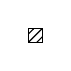
\begin{tikzpicture}[x=1.2ex,y=1.2ex]
        \filldraw[pattern=north east lines](0,0)rectangle(1,1);
      \end{tikzpicture} = Logistic,
      \begin{tikzpicture}[x=1.2ex,y=1.2ex]
        \filldraw[pattern=dots](0,0)rectangle(1,1);
    \end{tikzpicture} = MLP) \\
    \midrule
    & \multicolumn{4}{l}{Majority cl ass (Inflection)} & \otherchart{0.58}                  \\
    \hdashline
    & \chgform & –       & –        & –               & \chart{0.61}{0}{0.61}{0}     \\
    & –        & \chgemb & –        & –               & \chart{0.62}{0}{0.70}{0}     \\
    & –        & –       & \varform & –               & \chart{0.71}{0}{0.71}{0}     \\
    & –        & –       & –        & \varemb         & \chart{0.70}{0}{0.70}{0.0}     \\

    (A) & –        & –       & \varform & \varemb         & \chart{0.76}{0.0}{0.80}{0.0}     \\
    (B) & \chgform & \chgemb & –        & –               & \chart{0.60}{0.0}{0.67}{0.00}     \\
    (C) & \chgform & –       & \varform & –               & \chart{0.75}{0.0}{0.75}{0.0}     \\
    (D) & –        & \chgemb & –        & \varemb         & \chart{0.71}{0.0}{0.73}{0.0}     \\
    (E) & \chgform & \chgemb & \varform & \varemb         & \boldchart{0.79}{0.0}{0.85}{0.0} \\
    \arrayrulecolor{black}\bottomrule
  \end{tabularx}
  % \end{tabular}
  \caption{Accuracy in reconstructing UniMorph's inflection–derivation distinction by MLP classifiers using Word2Vec- vs. FastText-based distributional features. Hypotheses referred to in the main text are denoted with letters.}
  \label{tab:featresultsw2v}
\end{figure}

From the set of results in \cref{tab:featresultsw2v}, we do see non-trivial contributions of word-level distributional information, particularly for the $\varemb$ measure, even with this lower bound, indicating our FastText measure captures some semantic and syntactic information.
\chapter{Part II: Model performance by language}\label{app:performance}
See Table~\ref{tab:mperf} for per-language captioning performance, part-of-speech (POS) tagging accuracy, and perplexity of the base Gemma-2B model, the PaliGemma captioning model, and our fine-tuned language model (LM).
\def\mr#1{\multirow{2}{*}{#1}}
% make a shortcut to multicolumn
\def\mc#1#2{\multicolumn{#1}{c}{#2}}
% usage: \mc{2}{text}

\begin{landscape}
  {\small
    \renewcommand{\arraystretch}{1}

    \begin{longtable}{llrrrrrrrrrrrr}
\caption{Per-language performance metrics for the models used. A) CIDEr scores on Crossmodal-3600 (XM3600) and COCO-35L for the \texttt{paligemma-3b-ft-coco35-224} model. B) Perplexity scores for the base Gemma-2B model (Gemma), PaliGemma (PG) and our finetuned PaliGemma-based LM. As expected, PaliGemma has the lowest perplexity, and our fine-tuned model particularly improves perplexity on COCO-35L and for languages with different orthographies. C) Average POS tagging accuracy for the Stanza models on the Universal Dependencies treebank test sets for each language.}\label{tab:mperf}\\
\toprule
\cellcolor{white}\mr{Language} & \multirow{2}{1cm}[0em]{ISO 639-1}   &   \mc{2}{CIDEr}     &   \mc{3}{Perplexity (COCO-35L)} &   \mc{3}{Perplexity (XM3600)} &   \mc{3}{Perplexity (Multi30K)} & \multirow{2}{1.5cm}[0em]{Tagging Acc.}                                                                    \\
\cmidrule(lr){3-4}    \cmidrule(lr){5-7}              \cmidrule(lr){8-10}               \cmidrule(lr){11-13}
&            &   COCO-35L &   XM3600 &   Gemma &      PG &     FT-LM &   Gemma &       PG &      FT-LM &   Gemma     &      PG &   FT-LM &              \\
\midrule
\endfirsthead
\caption[]{Per-language performance metrics for the models used (continuted).}\label{tab:mperf}\\
\toprule

\mr{Language} & \multirow{2}{1cm}[0em]{ISO 639-1}   &   \mc{2}{CIDEr}     &   \mc{3}{Perplexity (COCO-35L)} &   \mc{3}{Perplexity (XM3600)} &   \mc{3}{Perplexity (Multi30K)} & \multirow{2}{1.5cm}[0em]{Tagging Acc.}                                                                    \\
\cmidrule(lr){3-4}    \cmidrule(lr){5-7}              \cmidrule(lr){8-10}               \cmidrule(lr){11-13}
&            &   COCO-35L &   XM3600 &   Gemma &      PG &     FT-LM &   Gemma &       PG &      FT-LM &   Gemma     &      PG &   FT-LM &              \\
\midrule
\endhead
Arabic        & \texttt{ar}         &    93.73 &     33.20 &    4.86 &     1.48 &       3.09 &   5.12 &    2.87 &      4.63 &   4.51      &    1.94 &   3.46  & 95.18        \\
Bengali       & \texttt{bn}         &    91.23 &     24.07 &    2.85 &     0.88 &       1.61 &   2.65 &    1.56 &      2.16 &   --        &    --    &   --     & --            \\
Czech         & \texttt{cs}         &    85.57 &     30.12 &    5.07 &     1.40 &       3.04 &   4.94 &    2.45 &      4.38 &   4.61      &    2.24 &   4.04  & 98.31        \\
Danish        & \texttt{da}         &   117.94 &     47.57 &    5.79 &     1.46 &       3.02 &   5.74 &    2.96 &      5.06 &   --        &    --    &   --     & 98.30        \\
German        & \texttt{de}         &    93.78 &     33.13 &    5.23 &     1.59 &       3.47 &   5.50 &    3.14 &      5.55 &   4.73      &    2.16 &   4.22  & 96.96        \\
Greek  & \texttt{el}      &   119.99 &     21.90 &   3.54 &    2.13 &      3.55 &    3.32 &     0.90 &       1.75 &   --        &    --    &   --     & 97.12        \\
English       & \texttt{en}         &   138.15 &     68.30 &    4.74 &     1.73 &       3.62 &   4.88 &    3.51 &      5.72 &   4.13      &    3.02 &   4.79  & 97.56        \\
Spanish       & \texttt{es}         &   138.51 &     48.69 &    4.85 &     1.55 &       3.36 &   5.40 &    3.23 &      5.51 &   --        &    --    &   --     & 98.01        \\
Persian       & \texttt{fa}         &   122.99 &     45.62 &    4.86 &     1.45 &       2.88 &   4.96 &    2.84 &      4.47 &   --        &    --    &   --     & 97.43        \\
Finnish       & \texttt{fi}         &    35.76 &     10.86 &    5.31 &     1.39 &       2.91 &   4.95 &    2.70 &      4.49 &   --        &    --    &   --     & 97.20        \\
French        & \texttt{fr}         &   137.79 &     53.35 &    4.96 &     1.44 &       3.15 &   5.13 &    3.12 &      5.08 &   4.36      &    2.73 &   4.50  & 97.55        \\
Hebrew        & \texttt{he}         &    97.94 &     36.59 &    4.36 &     1.34 &       2.71 &   3.84 &    2.30 &      3.74 &   --        &    --    &   --     & 90.84        \\
Hindi         & \texttt{hi}         &   104.52 &     26.98 &    3.75 &     1.19 &       2.28 &   3.86 &    2.68 &      3.54 &   --        &    --    &   --     & 97.95        \\
Croatian      & \texttt{hr}         &    89.42 &     25.95 &    5.24 &     1.37 &       2.88 &   4.68 &    2.49 &      4.33 &   --        &    --    &   --     & 98.21        \\
Hungarian     & \texttt{hu}         &    78.90 &     21.96 &    4.94 &     1.46 &       3.05 &   4.88 &    2.84 &      4.88 &   --        &    --    &   --     & 95.80        \\
Indonesian    & \texttt{id}         &   146.38 &     37.46 &    6.01 &     1.63 &       3.51 &   4.98 &    3.16 &      5.18 &   --        &    --    &   --     & 95.03        \\
Italian       & \texttt{it}         &   131.15 &     37.98 &    5.21 &     1.50 &       3.34 &   5.44 &    3.36 &      5.43 &   --        &    --    &   --     & 96.98        \\
Japanese      & \texttt{ja}         &   125.07 &     35.90 &    5.95 &     1.34 &       2.81 &   6.07 &    2.60 &      4.60 &   --        &    --    &   --     & 95.74        \\
Korean        & \texttt{ko}         &   112.40 &     42.82 &    4.89 &     1.29 &       2.61 &   4.80 &    2.37 &      3.95 &   --        &    --    &   --     & 95.86        \\
Norwegian     & \texttt{no}         &   118.02 &     39.67 &    6.13 &     1.50 &       3.07 &   5.70 &    2.90 &      4.75 &   --        &    --    &   --     & 98.38        \\
Dutch         & \texttt{nl}         &   114.76 &     47.19 &    4.96 &     1.54 &       3.24 &   5.34 &    3.15 &      5.55 &   --        &    --    &   --     & 96.71        \\
Polish        & \texttt{pl}         &    86.99 &     29.50 &    5.10 &     1.41 &       3.06 &   4.70 &    2.45 &      4.66 &   --        &    --    &   --     & 98.80        \\
Portuguese    & \texttt{pt}         &   136.40 &     42.76 &    5.52 &     1.53 &       3.30 &   5.56 &    3.38 &      5.49 &   --        &    --    &   --     & 97.74        \\
Romanian      & \texttt{ro}         &   118.57 &     22.36 &    5.15 &     1.30 &       2.73 &   4.62 &    2.63 &      4.18 &   --        &    --    &   --     & 97.98        \\
Russian       & \texttt{ru}         &    98.45 &     28.23 &    4.67 &     1.39 &       3.21 &   4.21 &    2.50 &      5.12 &   --        &    --    &   --     & 97.34        \\
Swedish       & \texttt{sv}         &   120.08 &     45.93 &    5.77 &     1.51 &       3.11 &   6.03 &    2.99 &      5.37 &   --        &    --    &   --     & 97.81        \\
Swahili       & \texttt{sw}         &   111.15 &     29.45 &    5.59 &     1.28 &       2.57 &   5.17 &    2.96 &      4.10 &   --        &    --    &   --     & --            \\
Maori         & \texttt{mi}         &   156.26 &     40.81 &    5.59 &     1.07 &       2.14 &   5.78 &    3.12 &      3.96 &   --        &    --    &   --     & --            \\
Telugu        & \texttt{te}         &    76.35 &     25.80 &    2.93 &     0.79 &       1.48 &   2.98 &    1.60 &      2.32 &   --        &    --    &   --     & 93.97        \\
Thai          & \texttt{th}         &   146.17 &     67.49 &    4.80 &     1.08 &       2.00 &   4.60 &    1.70 &      2.90 &   --        &    --    &   --     & --            \\
Turkish       & \texttt{tr}         &    86.26 &     27.58 &    6.05 &     1.62 &       3.42 &   5.61 &    3.00 &      5.00 &   --        &    --    &   --     & 95.26        \\
Ukrainian     & \texttt{uk}         &    92.90 &     22.47 &    4.26 &     1.23 &       2.67 &   4.01 &    2.48 &      4.38 &   --        &    --    &   --     & 97.52        \\
Vietnamese    & \texttt{vi}         &   159.82 &     51.57 &    4.83 &     1.48 &       3.02 &   4.66 &    3.02 &      4.86 &   --        &    --    &   --     & 81.48        \\
Chinese       & \texttt{zh}         &   103.19 &     26.41 &    6.01 &     1.55 &       3.21 &   5.86 &    3.06 &      4.97 &   --        &    --    &   --     & 88.82        \\
\bottomrule

\end{longtable}
}
\end{landscape}
\chapter{Groundedness correlation plots for other psycholinguistic norms}
Figure~\ref{fig:norms_extra} shows the relationship between our measure and concreteness, as well as the uncertainty coefficient, which normalizes our measure by the language model surprisal. While concreteness is most strongly associated with our measure/its normalized variant, for completeness we show the relationships between our measure and the other psycholinguistic norms (imageability and strength of visual experience) we investigate here.
\begin{figure*}
\centering

\begin{subfigure}{.49\textwidth}
\centering
\includegraphics[width=0.9\linewidth]{figures/grounded/imag_pmi.pdf}
\caption{$\rho=0.288$}
\label{fig:sub3}
\end{subfigure}
\begin{subfigure}{.49\textwidth}
\centering
\includegraphics[width=0.9\linewidth]{figures/grounded/imag_ratio.pdf}
\caption{$\rho=0.548$}
\label{fig:sub4}
\end{subfigure}
\begin{subfigure}{.49\textwidth}
\centering
\includegraphics[width=0.9\linewidth]{figures/grounded/visual_pmi.pdf}
\caption{$\rho=0.212$}
\label{fig:sub5}
\end{subfigure}
\begin{subfigure}{.49\textwidth}
\centering
\includegraphics[width=0.9\linewidth]{figures/grounded/visual_ratio.pdf}
\caption{$\rho=0.320$}
\label{fig:sub6}
\end{subfigure}
\caption{Correlation between English psycholinguistic norms  and type-level groundedness  (left) or uncertainty coefficent (right): i.e., the average ratio between LM surprisal and captioning model surprisal. Type-level measures were computed by averaging scores across the COCO-dev dataset for types which occur at least 30 times.}
\label{fig:norms_extra}
\end{figure*}
\chapter{Groundedness distributions by language and dataset}
\section{Crossmodal-3600}\label{results:xm}
Results are ordered by descending mutual information estimate within the dataset (average groundedness/PMI). Hue indicates the average cross-linguistic ranking of a part of speech.

\vspace{3em}
\noindent
\foreach \langtwo in {ar,cs,da,de,el,en,es,fa,fi,fr,he,hi,hr,hu,id,it,ja,ko,nl,no,pl,pt,ro,ru,sv,te,tr,uk,vi,zh} {
\includegraphics[width=\linewidth]{figures/xm3600-2/pos_\langtwo.pdf}
%\caption{Word-token-level distribution of PMIs for \texttt{\lang}}
}
\section{Multi30K}\label{results:multi}
Results are ordered by descending mutual information estimate within the dataset (average groundedness/PMI). Hue indicates the average cross-linguistic ranking of a part of speech.

\vspace{3em}
\noindent
\foreach \langthree in {ar,cs,de,en,fr} {
\includegraphics[width=\linewidth]{figures/multi30k/pos_\langthree.pdf}
%\caption{Word-token-level distribution of PMIs for \texttt{\lang}}
}

\section{COCO-35L Development Set}\label{results:coco}
Results are ordered by descending mutual information estimate within the dataset (average groundedness/PMI). Hue indicates the average cross-linguistic ranking of a part of speech.

\vspace{3em}
\noindent
\foreach \lang in {ar,cs,da,de,el,en,es,fa,fi,fr,he,hi,hr,hu,id,it,ja,ko,nl,no,pl,pt,ro,ru,sv,te,tr,uk,vi,zh} {
\includegraphics[width=\linewidth]{figures/coco35/pos_\lang.pdf}
}
%% Choose your favourite bibliography style here.
\bibliographystyle{acl_natbib}
% \bibliographystyle{acm}

%% If you want the bibliography single-spaced (which is allowed), uncomment
%% the next line.
%\singlespace

\bibliography{thesis,anthology}

\end{document}
